
% Choose the language of your thesis passing 'french' or 'english' as
% \documentclass option.
% Note1: The 'page de garde' will always be written in French.
% Note2: You will have an error if you change the language of the document and
%        compile it without cleaning the auxiliary files. Compiling it again
%        should solve the problem.
\documentclass[english,a4paper,11pt,twoside]{StyleThese}
\newcommand{\included}{}




\usepackage{amsmath,amssymb, amsthm}             % AMS Math
\usepackage[T1]{fontenc}
\usepackage[utf8x]{inputenc}
\usepackage{babel}
\usepackage{datetime}

\usepackage{silence}

\WarningFilter{minitoc(hints)}{W0023}
\WarningFilter{minitoc(hints)}{W0028}
\WarningFilter{minitoc(hints)}{W0030}

\usepackage{lmodern}
\usepackage{tabularx}
%\usepackage{tabular}
\usepackage{multirow}
\usepackage{xspace}

\usepackage{subfig}
\usepackage[inline]{enumitem}

\usepackage{hhline}
\usepackage[left=1.5in,right=1.3in,top=1.1in,bottom=1.1in,includefoot,includehead,headheight=13.6pt]{geometry}
\renewcommand{\baselinestretch}{1.05}

% Table of contents for each chapter

\usepackage[nottoc, notlof, notlot]{tocbibind}
\usepackage{minitoc}
\setcounter{minitocdepth}{2}
\mtcindent=15pt
% Use \minitoc where to put a table of contents

\usepackage{aecompl}

% Glossary / list of abbreviations

\usepackage[intoc]{nomencl}
\iftoggle{ThesisInEnglish}{%
\renewcommand{\nomname}{Glossary}
}{ %
\renewcommand{\nomname}{Liste des Abréviations}
}

\usepackage{etoolbox}
\renewcommand\nomgroup[1]{%
  \item[\bfseries
  \ifstrequal{#1}{A}{Number Sets}{%
  \ifstrequal{#1}{G}{Agents Beliefs and Action Models}{%
  \ifstrequal{#1}{N}{Navigation}{%
  \ifstrequal{#1}{O}{Ontology}{%
  \ifstrequal{#1}{R}{Referring Expression Generation}{%
  \ifstrequal{#1}{Z}{Controllable and Uncontrollable Agents Task Planning}{}}}}}}%
]}

\makenomenclature



% My pdf code

\usepackage{ifpdf}

\ifpdf
  \usepackage[pdftex]{graphicx}
  \DeclareGraphicsExtensions{.jpg}
  \usepackage[pagebackref,hyperindex=true]{hyperref}
  \usepackage{tikz}
  \usetikzlibrary{arrows,shapes,calc}
\else
  \usepackage{graphicx}
  \DeclareGraphicsExtensions{.ps,.eps}
  \usepackage[dvipdfm,pagebackref,hyperindex=true]{hyperref}
\fi

\graphicspath{{.}{images/}}

%% nicer backref links. NOTE: The flag ThesisInEnglish is used to define the
% language in the back references. Read more about it in These.tex

\iftoggle{ThesisInEnglish}{%
\renewcommand*{\backref}[1]{}
\renewcommand*{\backrefalt}[4]{%
\ifcase #1 %
(Not cited.)%
\or
(Cited in page~#2.)%
\else
(Cited in pages~#2.)%
\fi}
\renewcommand*{\backrefsep}{, }
\renewcommand*{\backreftwosep}{ and~}
\renewcommand*{\backreflastsep}{ and~}
}{%
\renewcommand*{\backref}[1]{}
\renewcommand*{\backrefalt}[4]{%
\ifcase #1 %
(Non cité.)%
\or
(Cité en page~#2.)%
\else
(Cité en pages~#2.)%
\fi}
\renewcommand*{\backrefsep}{, }
\renewcommand*{\backreftwosep}{ et~}
\renewcommand*{\backreflastsep}{ et~}
}

% Links in pdf
\usepackage{color}
\definecolor{linkcol}{rgb}{0,0,0.4} 
\definecolor{citecol}{rgb}{0.5,0,0} 
\definecolor{linkcol}{rgb}{0,0,0} 
\definecolor{citecol}{rgb}{0,0,0}
% Change this to change the informations included in the pdf file

\hypersetup
{
bookmarksopen=true,
pdftitle="Endowing the robot with the abilities to control and evaluate its contribution to a human-robot joint action",
pdfauthor="Amandine MAYIMA", %auteur du document
pdfsubject="Thèse", %sujet du document
%pdftoolbar=false, %barre d'outils non visible
pdfmenubar=true, %barre de menu visible
pdfhighlight=/O, %effet d'un clic sur un lien hypertexte
colorlinks=true, %couleurs sur les liens hypertextes
pdfpagemode=None, %aucun mode de page
pdfpagelayout=SinglePage, %ouverture en simple page
pdffitwindow=true, %pages ouvertes entierement dans toute la fenetre
linkcolor=linkcol, %couleur des liens hypertextes internes
citecolor=citecol, %couleur des liens pour les citations
urlcolor=linkcol %couleur des liens pour les url
}

% definitions.
% -------------------

\setcounter{secnumdepth}{3}
\setcounter{tocdepth}{2}

% Some useful commands and shortcut for maths:  partial derivative and stuff

\newcommand{\pd}[2]{\frac{\partial #1}{\partial #2}}
\def\abs{\operatorname{abs}}
\def\argmax{\operatornamewithlimits{arg\,max}}
\def\argmin{\operatornamewithlimits{arg\,min}}
\def\diag{\operatorname{Diag}}
\newcommand{\eqRef}[1]{(\ref{#1})}

\usepackage{rotating}                    % Sideways of figures & tables
%\usepackage{bibunits}
%\usepackage[sectionbib]{chapterbib}          % Cross-reference package (Natural BiB)
%\usepackage{natbib}                  % Put References at the end of each chapter
                                         % Do not put 'sectionbib' option here.
                                         % Sectionbib option in 'natbib' will do.
\usepackage{fancyhdr}                    % Fancy Header and Footer

% \usepackage{txfonts}                     % Public Times New Roman text & math font
  
%%% Fancy Header %%%%%%%%%%%%%%%%%%%%%%%%%%%%%%%%%%%%%%%%%%%%%%%%%%%%%%%%%%%%%%%%%%
% Fancy Header Style Options

\pagestyle{fancy}                       % Sets fancy header and footer
\fancyfoot{}                            % Delete current footer settings

%\renewcommand{\chaptermark}[1]{         % Lower Case Chapter marker style
%  \markboth{\chaptername\ \thechapter.\ #1}}{}} %

%\renewcommand{\sectionmark}[1]{         % Lower case Section marker style
%  \markright{\thesection.\ #1}}         %

\fancyhead[LE,RO]{\bfseries\thepage}    % Page number (boldface) in left on even
% pages and right on odd pages
\fancyhead[RE]{\bfseries\nouppercase{\leftmark}}      % Chapter in the right on even pages
\fancyhead[LO]{\bfseries\nouppercase{\rightmark}}     % Section in the left on odd pages

\let\headruleORIG\headrule
\renewcommand{\headrule}{\color{black} \headruleORIG}
\renewcommand{\headrulewidth}{1.0pt}
\usepackage{colortbl}
\arrayrulecolor{black}

\fancypagestyle{plain}{
  \fancyhead{}
  \fancyfoot{}
  \renewcommand{\headrulewidth}{0pt}
}

%\usepackage{MyAlgorithm}
%\usepackage[noend]{MyAlgorithmic}
\usepackage{algorithm}
\usepackage[noend]{algpseudocode}
\usepackage{comment}
\usepackage[ED=MITT-InfoTel, Ets=INSA]{tlsflyleaf}
%%% Clear Header %%%%%%%%%%%%%%%%%%%%%%%%%%%%%%%%%%%%%%%%%%%%%%%%%%%%%%%%%%%%%%%%%%
% Clear Header Style on the Last Empty Odd pages
\makeatletter

\def\cleardoublepage{\clearpage\if@twoside \ifodd\c@page\else%
  \hbox{}%
  \thispagestyle{empty}%              % Empty header styles
  \newpage%
  \if@twocolumn\hbox{}\newpage\fi\fi\fi}

\newcommand*{\algrule}[1][\algorithmicindent]{%
	\makebox[#1][l]{%
		\hspace*{.2em}% <------------- This is where the rule starts from
		\vrule height .75\baselineskip depth .25\baselineskip
	}
}

%%% to have lines in algorithm, from stackexchange
\newcount\ALG@printindent@tempcnta
\def\ALG@printindent{%
	\ifnum \theALG@nested>0% is there anything to print
	\ifx\ALG@text\ALG@x@notext% is this an end group without any text?
	% do nothing
	\else
	\unskip
	% draw a rule for each indent level
	\ALG@printindent@tempcnta=1
	\loop
	\algrule[\csname ALG@ind@\the\ALG@printindent@tempcnta\endcsname]%
	\advance \ALG@printindent@tempcnta 1
	\ifnum \ALG@printindent@tempcnta<\numexpr\theALG@nested+1\relax
	\repeat
	\fi
	\fi
}
% the following line injects our new indent handling code in place of the default spacing
\patchcmd{\ALG@doentity}{\noindent\hskip\ALG@tlm}{\ALG@printindent}{}{\errmessage{failed to patch}}
\patchcmd{\ALG@doentity}{\item[]\nointerlineskip}{}{}{} % no spurious vertical space
% end vertical rule patch for algorithmicx

\makeatother
 
%%%%%%%%%%%%%%%%%%%%%%%%%%%%%%%%%%%%%%%%%%%%%%%%%%%%%%%%%%%%%%%%%%%%%%%%%%%%%%% 
% Prints your review date and 'Draft Version' (From Josullvn, CS, CMU)
\newcommand{\reviewtimetoday}[2]{\special{!userdict begin
    /bop-hook{gsave 20 710 translate 45 rotate 0.8 setgray
      /Times-Roman findfont 12 scalefont setfont 0 0   moveto (#1) show
      0 -12 moveto (#2) show grestore}def end}}
% You can turn on or off this option.
% \reviewtimetoday{\today}{Draft Version}
%%%%%%%%%%%%%%%%%%%%%%%%%%%%%%%%%%%%%%%%%%%%%%%%%%%%%%%%%%%%%%%%%%%%%%%%%%%%%%% 

\newenvironment{maxime}[1]
{
\vspace*{0cm}
\hfill
\begin{minipage}{0.5\textwidth}%
%\rule[0.5ex]{\textwidth}{0.1mm}\\%
\hrulefill $\:$ {\bf #1}\\
%\vspace*{-0.25cm}
\it 
}%
{%

\hrulefill
\vspace*{0.5cm}%
\end{minipage}
}

\let\minitocORIG\minitoc
\renewcommand{\minitoc}{\minitocORIG \vspace{1.5em}}

\usepackage{multirow}
%\usepackage{slashbox}

\newenvironment{bulletList}%
{ \begin{list}%
	{\tiny$\bullet$}%
	{\setlength{\labelwidth}{25pt}%
	 \setlength{\leftmargin}{30pt}%
	 \setlength{\itemsep}{-0.5em}}}%
{ \end{list} }

\newenvironment{inlineEnumerate}
{\begin{enumerate*} [label={(\arabic*)}] }
{\end{enumerate*}}

\theoremstyle{definition}
\newtheorem{definition}{Definition}
\renewcommand{\epsilon}{\varepsilon}

% centered page environment

\newenvironment{vcenterpage}
{\newpage\vspace*{\fill}\thispagestyle{empty}\renewcommand{\headrulewidth}{0pt}}
{\vspace*{\fill}}

\newenvironment{asl}{\ttfamily\begin{tabbing}~~~\=$\leftarrow$ \= ~~~ \=
		\kill}{\end{tabbing}}

\usepackage{tablefootnote}

\theoremstyle{plain}
\newtheorem{constraint}{Constraint}[section]

\algnewcommand\algorithmicforeach{\textbf{for each}}
\algnewcommand\algorithmicin{\textbf{in}}
\algdef{S}[FOR]{ForEach}[2]{\algorithmicforeach\ #1\ \algorithmicin\ #2\ \algorithmicdo}

\algnewcommand\algorithmicforkxor{\textbf{do fork-join-xor}}
\algnewcommand\algorithmicendforkxor{\textbf{end fork-join-xor}}
\algdef{SE}{ForkXor}{EndForkXor}{\algorithmicforkxor}{\algorithmicendforkxor}


\usepackage{listings}
\lstset{
	frame=single,
	captionpos=b,
	breaklines=true,
	basicstyle=\ttfamily,
	numberstyle=\color{black},
	tabsize=2,
	mathescape=true,
	literate=%
		{â}{{\^a}}1
}

\lstdefinestyle{inline}{
	frame=none,
	aboveskip=\smallskipamount,
	belowskip=\smallskipamount,
}

\lstdefinestyle{OwlTurtle}{
	language=C,
	tabsize=4,
	basicstyle=\scriptsize\ttfamily,
	keywordstyle=\bfseries\color{darkgray},
	morekeywords={rdf:type, rdfs:domain, rdfs:subPropertyOf, rdfs:range, :hasSubtask, :DecompositionUsedBy, rdfs:subClassOf, :hasDecomposition, owl:inverseOf, htn_actions:hasEffect, rdfs:label},
	alsoletter=:
}

\lstdefinestyle{aslDef}{
	frame=none,
%	breaklines=false,
	%xleftmargin=.1\textwidth, xrightmargin=.1\textwidth
}

\fancypagestyle{example}{%
	\fancyhead[LE]{\bfseries\thepage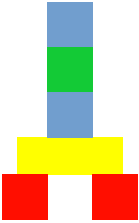
\includegraphics[scale=0.20]{figures/chapter2/task_goal.pdf}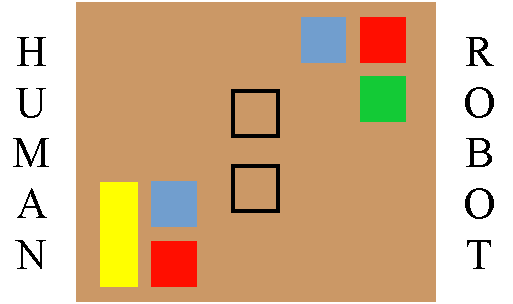
\includegraphics[scale=0.18]{figures/chapter2/task_setup_mini.pdf}}   
	\fancyhead[RO]{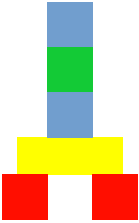
\includegraphics[scale=0.20]{figures/chapter2/task_goal.pdf}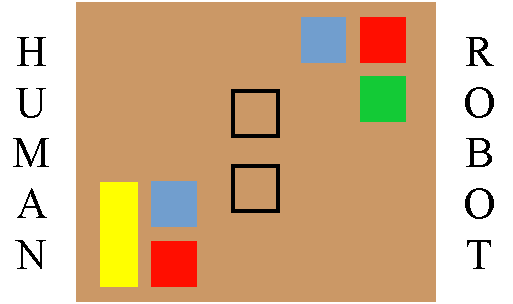
\includegraphics[scale=0.18]{figures/chapter2/task_setup_mini.pdf}\bfseries\thepage}  
	\fancyhead[RE]{\bfseries\nouppercase{\leftmark}}      % Chapter in the right on even pages
	\fancyhead[LO]{\bfseries\nouppercase{\rightmark}}     % Section in the left on odd pages
}%

\usepackage{pdfpages}
\usepackage{makecell}
\usepackage{pdflscape} 
\usepackage{mathtools}
\usepackage[section]{placeins}
\usepackage{afterpage}

%%%%%%%% my commands
\newcommand{\etal}{\textit{et al}.}
\newcommand{\ie}{\textit{i.e.}, }
\newcommand{\eg}{\textit{e.g.}, }
\newcommand{\fact}[3]{\mbox{\textit{#1}(#2, #3)}}
\newcommand{\circledtext}[1]{\raisebox{.5pt}{\textcircled{\raisebox{-.9pt} {#1}}}}
\newcommand{\sparql}{\textsc{SPARQL}}

\newcommand{\algConst}[1]{${\scriptscriptstyle #1}$}
\newcommand{\algNormTextSub}[2]{$\text{#1}_{#2}$}

\newcommand{\aslnumber}[1]{$#1$}
\newcommand{\aslstring}[1]{\textsf{#1}}
\newcommand{\aslvar}[1]{\textcolor{purple}{\textit{#1}}}
\newcommand{\asllabel}[1]{\textbf{#1}}
\newcommand{\annotation}[1]{{\footnotesize #1}}
\newcommand{\rulebody}[1]{\mbox{\hspace{.05\linewidth}}\begin{minipage}[t]{0.9\linewidth}#1.\end{minipage}}
\newcommand{\context}[1]{\begin{minipage}[t]{0.9\linewidth}#1\end{minipage}}
\newcommand{\planbody}[1]{\begin{minipage}[t]{0.9\linewidth}#1.\end{minipage}}
\newcommand{\Jason}[0]{\textbf{\textit{Jason}}}
\newcommand{\sn}{\mbox{\large\textbf{\texttt{\textasciitilde}}}}


\usepackage[acronym]{glossaries}

\makenoidxglossaries

\newacronym{bdi}{BDI}{Belief-Desire-Intention}
\newacronym{hateb}{HATEB}{Human-Aware Timed Elastic Bands}
\newacronym{hri}{HRI}{Human Robot Interaction}
\newacronym{hci}{HCI}{Human Computer Interaction}
\newacronym{jahrvis}{JAHRVIS}{Joint Action-based Human-Aware supeRVISor}
\newacronym{htn}{HTN}{Hierarchical Task Network}
\newacronym{hatp}{HATP}{Hierarchical Agent-based Task Planner}
\newacronym{reg}{REG}{Referring Expression Generation}
\newacronym{re}{RE}{Referring Expression}
\newacronym{teb}{TEB}{Timed Elastic Band}
\newacronym{kb}{KB}{Knowledge Base}
\newacronym{mummer}{MuMMER}{MultiModal Mall Entertainment Robot}
\newacronym{clle}{CLLE}{Cognition, Langues, Langage, Ergonomie}
\newacronym{ttc}{TTC}{Time-to-Collision}
\newacronym{ux}{UX}{User Experience}
\newacronym{perdita}{PeRDITA}{Pertinence of Robot Decisions In joinT Action}
\newacronym{hatpehda}{HATP/EHDA}{Human Aware Task Planner with Emulation of Human Decisions and Actions}
\newacronym{ssr}{SSR}{Semantic Spatial Representation}
\newacronym{rja}{RJA}{ROS-Jason Agent}
\newacronym{ham}{HAM}{Human Actions Monitoring}
\newacronym{hpm}{HPM}{Human Plan Manager}
\newacronym{tom}{ToM}{Theory of Mind}

%\nomenclature[A]{$\realset$}{Real Numbers}
%\nomenclature[A]{$\intset$}{Natural Numbers}
%
%\nomenclature[G]{$\robotmodel$}{The generic model of the robot has of itself. It can include action models or knowledge}
%\nomenclature[G]{$\humanmodel$}{The generic model of the human given to the robot. It can include action models or knowledge}
%\nomenclature[G]{$\robotinhumanmodel$}{The generic estimation of the model of the robot the human has. It can include action models or knowledge}
%
%\nomenclature[N]{$\robotband$}{The robot elastic band used in HATEB}
%\nomenclature[N]{$\humanband$}{The human elastic band used in HATEB}
%
%\nomenclature[O]{$\knowledgebase$}{The knowledge base (ontology)}
%\nomenclature[O]{$\abox$}{The ABox of the ontology}
%\nomenclature[O]{$\tbox$}{The TBox of the ontology}
%\nomenclature[O]{$\rbox$}{The RBox of the ontology}
%\nomenclature[O]{$\indivset$}{The set of entities in the ontology}
%\nomenclature[O]{$\classset$}{The set of classes in the ontology}
%\nomenclature[O]{$\relationset$}{The set of relations in the ontology}
%\nomenclature[O]{$\relationset$}{The set of relations in the ontology}
%
%\nomenclature[R]{$\variableset$}{The set of variables used in the \sparql{} queries and in referring expressions}
%\nomenclature[R]{$\labelfunc$}{The labeling function}
%\nomenclature[R]{$\costcompfunc$}{The properties interpretation cost function}
%\nomenclature[R]{$\goalindiv$}{The target entity, the entity to generate a referring expression for}
%\nomenclature[R]{$\usablepropset$}{The set of usable properties for the referring expression generation problem}
%\nomenclature[R]{$\regproblem$}{The referring expression generation problem}
%\nomenclature[R]{$\node$}{A node of the search space graph for the referring expression generation}
%\nomenclature[R]{$\transition$}{A transition of the search space graph for the referring expression generation}
%\nomenclature[R]{$\softdiff$}{The soft difference function, returning a list of relations from two entities}
%\nomenclature[R]{$\harddiff$}{The hard difference function, returning a list of relations from two entities}
%
%\nomenclature[Z]{$\statespace$}{The set of all the possible world states (beliefs)}
%\nomenclature[Z]{$\agents$}{The set of the agents (controllable and uncontrollable) considered during the planning}
%\nomenclature[Z]{$\agentstate$}{A state of an agent, containing their agenda, (partial) plan and beliefs}
%\nomenclature[Z]{$\ctrlagents$}{The set of controllable agents (robots)}
%\nomenclature[Z]{$\unctrlagents$}{The set of uncontrollable agents (humans)}
%\nomenclature[Z]{$\agentsstates$}{The union of the state of all the agents considered by the planner}
%\nomenclature[Z]{$\agentsstatesset$}{The set of all the possible states of all the agents considered by the planner}
%\nomenclature[Z]{$\actionmodel$}{The action model of an agent}
%\nomenclature[Z]{$\operators$}{The set of primitive tasks of an agent}
%\nomenclature[Z]{$\abstracttasks$}{The set of abstract tasks of an agent}
%\nomenclature[Z]{$\methods$}{The set of methods of an agent}
%\nomenclature[Z]{$\agenda$}{The agenda of an agent}
%\nomenclature[Z]{$\plan$}{The (partial) plan (execution stream) of an agent}
%\nomenclature[Z]{$\triggerset$}{The set of trigger functions of an agent}
%\nomenclature[Z]{$\Pi$}{A conditional plan}

%\nomenclature{HRI}{Human Robot Interaction}
%\nomenclature{REG}{Referring Expression Generation}
%\nomenclature{RE}{Referring Expression}
%\nomenclature{TEB}{Timed Elastic Band}
%\nomenclature{HATEB}{Human-Aware Timed Elastic Bands}

\usepackage{xargs}                      % Use more than one optional parameter in a new commands
\usepackage{xcolor}  % Coloured text etc.
% 
\usepackage[colorinlistoftodos,prependcaption,textsize=tiny]{todonotes}
%\usepackage[disable,colorinlistoftodos,prependcaption,textsize=tiny]{todonotes}
\setlength{\marginparwidth}{3cm}
\newcommandx{\unsure}[2][1=]{\todo[linecolor=red,backgroundcolor=red!25,bordercolor=red,#1]{#2}}
\newcommandx{\change}[2][1=]{\todo[linecolor=blue,backgroundcolor=blue!25,bordercolor=blue,#1]{#2}}
\newcommandx{\info}[2][1=]{\todo[linecolor=olive,backgroundcolor=olive!25,bordercolor=olive,#1]{#2}}
\newcommandx{\improvement}[2][1=]{\todo[linecolor=violet,backgroundcolor=violet!25,bordercolor=violet,#1]{#2}}
\newcommandx{\thiswillnotshow}[2][1=]{\todo[disable,#1]{#2}}

%%%%% Chapter 1
\newcommand{\robotmodel}{\mathcal{M}^R}
\newcommand{\humanmodel}{\mathcal{M}^H_r}
\newcommand{\robotinhumanmodel}{\mathcal{M}^R_h}


%%%%% Chapter 2
\newcommand{\realset}{\mathbb{R}}
\newcommand{\intset}{\mathbb{N}}
\newcommand{\robotband}{B_\mathcal{R}}
\newcommand{\humanband}{B_\mathcal{H}}

%%%%% Chapter 3
\newcommand{\knowledgebase}{K}
\newcommand{\abox}{\mathcal{A}}
\newcommand{\tbox}{\mathcal{T}}
\newcommand{\rbox}{\mathcal{R}}
\newcommand{\variableset}{X}
\newcommand{\labelfunc}{\mathcal{L}}
\newcommand{\costcompfunc}{\mathcal{C}}
\newcommand{\indivset}{A}
\newcommand{\classset}{T}
\newcommand{\indiv}{a}
\newcommand{\class}{t}
\newcommand{\relationset}{R}
\newcommand{\goalindiv}{a_t}
\newcommand{\usablepropset}{U}
\newcommand{\regproblem}{REG}
\newcommand{\node}{\mathfrak{n}}
\newcommand{\transition}{\mathfrak{t}}
\newcommand{\sparql}{\textsc{SparQL}}
\newcommand{\softdiff}{\,\delta\,}
\newcommand{\harddiff}{\,\Delta\,}

%%%%% Chapter 4
\newcommand{\statespace}{S}
\newcommand{\worldstate}{s}
\newcommand{\agent}{\alpha}
\newcommand{\agents}{Ag}
\newcommand{\agentstate}{\sigma}
\newcommand{\ctrlagents}{\widehat{Ag}}
\newcommand{\unctrlagents}{\widetilde{Ag}}
\newcommand{\agentsstates}{\sigma}
\newcommand{\ctrlagentsstates}{\widehat{\sigma}}
\newcommand{\unctrlagentsstates}{\widetilde{\sigma}}
\newcommand{\agentsstatesset}{\Sigma}
\newcommand{\actionmodel}{\Lambda}
\newcommand{\operators}{Op}
\newcommand{\abstracttasks}{Ab}
\newcommand{\methods}{Me}
\newcommand{\agenda}{d}
\newcommand{\plan}{\pi}
\newcommand{\triggerset}{Tr}
\newcommand{\policy}{\Pi}

%%%%%
% À mettre dans le préambule (avant \begin{document})
%%%%%
%% Titre, auteur, date, laboratoire, cotutelle
\title{Endowing the Robot with the Abilities to Control and Evaluate its Contribution to a Human-Robot Joint Action}
\author{Amandine MAYIMA}
\defencedate{29/10/2021}
\lab{Laboratoire d'Analyse et d'Architecture des Systèmes (LAAS-CNRS)}
%\cotutelle{Institut de cotutelle}

%% Directeur(s) de thèse
\nboss{2}                                    % Nombre de directeur(s) de thèse
\makesomeone{boss}{2}{Aurélie CLODIC}{}{}  % Sera affiché en second
\makesomeone{boss}{1}{Rachid ALAMI}{}{} % Sera affiché en premier
%% Referee
\nreferee{2}
\makesomeone{referee}{1}{Silvia ROSSI}{}{}
\makesomeone{referee}{2}{Peter Ford DOMINEY}{}{}
%% Jury
\njudge{7}
%\makesomeone{judge}{1}{???}{Professeur}{Président du Jury}
\makesomeone{judge}{2}{Silvia ROSSI}{Professeure Associée}{Rapporteure}
\makesomeone{judge}{3}{Peter Ford DOMINEY}{Directeur de Recherche}{Rapporteur}
\makesomeone{judge}{7}{Rachid ALAMI}{Directeur de Recherche}{Directeur de Thèse}
\makesomeone{judge}{6}{Aurélie CLODIC}{Ingénieure de Recherche}{Directrice de Thèse}
\makesomeone{judge}{1}{Simon LACROIX}{Directeur de Recherche}{Président du Jury}
\makesomeone{judge}{4}{Guy HOFFMAN}{Professeur Associé}{Membre du Jury}
\makesomeone{judge}{5}{Elisabeth PACHERIE}{Directrice de Recherche}{Membre du Jury}
%% Quel ordre ?

\sloppy
\begin{document}
\makeflyleaf

\cleardoublepage

\dominitoc

\pagenumbering{roman}

 \cleardoublepage

% Here you can see an example of how to create text conditioned by the language
% variable. The \iftoggle command:
%
%   \iftoggle{ThesisInEnglish}{%
%   <your-text-in-english>
%   }{%
%   <your-text-in-french>
%   }
%
% will compile only one of the two blocks, depending on the variable you set at
% the beginning of this document. Language selection is managed this way in the
% formatAndDefs.tex file. You too can create sections of your thesis that is
% language dependend this way, although you probably won't need it. Another use
% of \iftoggle can be found at the end of this file.
\iftoggle{ThesisInEnglish}{%
\section*{Acknowledgments}
}{%
\section*{Remerciements}
}

A faire en dernier :-) 

\tableofcontents

%\printnomenclature
\printnoidxglossary[type=\acronymtype]
% Use \mtcfixnomenclature below if you have a glossary (added with
% \printnomenclature above) and you're see a shift in the mini-table of
% contents at the begining of each chapter (example: no mini-toc in chapter 1;
% mini-toc of chapter 1 appearing in chapter 2; and so on).
%
% You should not use \mtcfixnomenclature if you have no glossary (that means,
% if you don't use \printnomenclature or if your glossary is empty).
%\mtcfixnomenclature

\mainmatter

\ifdefined\included
\else
\documentclass[a4paper,11pt,twoside]{StyleThese}
\usepackage{amsmath,amssymb, amsthm}             % AMS Math
\usepackage[T1]{fontenc}
\usepackage[utf8x]{inputenc}
\usepackage{babel}
\usepackage{datetime}

\usepackage{silence}

\WarningFilter{minitoc(hints)}{W0023}
\WarningFilter{minitoc(hints)}{W0028}
\WarningFilter{minitoc(hints)}{W0030}

\usepackage{lmodern}
\usepackage{tabularx}
%\usepackage{tabular}
\usepackage{multirow}
\usepackage{xspace}

\usepackage{subfig}
\usepackage[inline]{enumitem}

\usepackage{hhline}
\usepackage[left=1.5in,right=1.3in,top=1.1in,bottom=1.1in,includefoot,includehead,headheight=13.6pt]{geometry}
\renewcommand{\baselinestretch}{1.05}

% Table of contents for each chapter

\usepackage[nottoc, notlof, notlot]{tocbibind}
\usepackage{minitoc}
\setcounter{minitocdepth}{2}
\mtcindent=15pt
% Use \minitoc where to put a table of contents

\usepackage{aecompl}

% Glossary / list of abbreviations

\usepackage[intoc]{nomencl}
\iftoggle{ThesisInEnglish}{%
\renewcommand{\nomname}{Glossary}
}{ %
\renewcommand{\nomname}{Liste des Abréviations}
}

\usepackage{etoolbox}
\renewcommand\nomgroup[1]{%
  \item[\bfseries
  \ifstrequal{#1}{A}{Number Sets}{%
  \ifstrequal{#1}{G}{Agents Beliefs and Action Models}{%
  \ifstrequal{#1}{N}{Navigation}{%
  \ifstrequal{#1}{O}{Ontology}{%
  \ifstrequal{#1}{R}{Referring Expression Generation}{%
  \ifstrequal{#1}{Z}{Controllable and Uncontrollable Agents Task Planning}{}}}}}}%
]}

\makenomenclature



% My pdf code

\usepackage{ifpdf}

\ifpdf
  \usepackage[pdftex]{graphicx}
  \DeclareGraphicsExtensions{.jpg}
  \usepackage[pagebackref,hyperindex=true]{hyperref}
  \usepackage{tikz}
  \usetikzlibrary{arrows,shapes,calc}
\else
  \usepackage{graphicx}
  \DeclareGraphicsExtensions{.ps,.eps}
  \usepackage[dvipdfm,pagebackref,hyperindex=true]{hyperref}
\fi

\graphicspath{{.}{images/}}

%% nicer backref links. NOTE: The flag ThesisInEnglish is used to define the
% language in the back references. Read more about it in These.tex

\iftoggle{ThesisInEnglish}{%
\renewcommand*{\backref}[1]{}
\renewcommand*{\backrefalt}[4]{%
\ifcase #1 %
(Not cited.)%
\or
(Cited in page~#2.)%
\else
(Cited in pages~#2.)%
\fi}
\renewcommand*{\backrefsep}{, }
\renewcommand*{\backreftwosep}{ and~}
\renewcommand*{\backreflastsep}{ and~}
}{%
\renewcommand*{\backref}[1]{}
\renewcommand*{\backrefalt}[4]{%
\ifcase #1 %
(Non cité.)%
\or
(Cité en page~#2.)%
\else
(Cité en pages~#2.)%
\fi}
\renewcommand*{\backrefsep}{, }
\renewcommand*{\backreftwosep}{ et~}
\renewcommand*{\backreflastsep}{ et~}
}

% Links in pdf
\usepackage{color}
\definecolor{linkcol}{rgb}{0,0,0.4} 
\definecolor{citecol}{rgb}{0.5,0,0} 
\definecolor{linkcol}{rgb}{0,0,0} 
\definecolor{citecol}{rgb}{0,0,0}
% Change this to change the informations included in the pdf file

\hypersetup
{
bookmarksopen=true,
pdftitle="Endowing the robot with the abilities to control and evaluate its contribution to a human-robot joint action",
pdfauthor="Amandine MAYIMA", %auteur du document
pdfsubject="Thèse", %sujet du document
%pdftoolbar=false, %barre d'outils non visible
pdfmenubar=true, %barre de menu visible
pdfhighlight=/O, %effet d'un clic sur un lien hypertexte
colorlinks=true, %couleurs sur les liens hypertextes
pdfpagemode=None, %aucun mode de page
pdfpagelayout=SinglePage, %ouverture en simple page
pdffitwindow=true, %pages ouvertes entierement dans toute la fenetre
linkcolor=linkcol, %couleur des liens hypertextes internes
citecolor=citecol, %couleur des liens pour les citations
urlcolor=linkcol %couleur des liens pour les url
}

% definitions.
% -------------------

\setcounter{secnumdepth}{3}
\setcounter{tocdepth}{2}

% Some useful commands and shortcut for maths:  partial derivative and stuff

\newcommand{\pd}[2]{\frac{\partial #1}{\partial #2}}
\def\abs{\operatorname{abs}}
\def\argmax{\operatornamewithlimits{arg\,max}}
\def\argmin{\operatornamewithlimits{arg\,min}}
\def\diag{\operatorname{Diag}}
\newcommand{\eqRef}[1]{(\ref{#1})}

\usepackage{rotating}                    % Sideways of figures & tables
%\usepackage{bibunits}
%\usepackage[sectionbib]{chapterbib}          % Cross-reference package (Natural BiB)
%\usepackage{natbib}                  % Put References at the end of each chapter
                                         % Do not put 'sectionbib' option here.
                                         % Sectionbib option in 'natbib' will do.
\usepackage{fancyhdr}                    % Fancy Header and Footer

% \usepackage{txfonts}                     % Public Times New Roman text & math font
  
%%% Fancy Header %%%%%%%%%%%%%%%%%%%%%%%%%%%%%%%%%%%%%%%%%%%%%%%%%%%%%%%%%%%%%%%%%%
% Fancy Header Style Options

\pagestyle{fancy}                       % Sets fancy header and footer
\fancyfoot{}                            % Delete current footer settings

%\renewcommand{\chaptermark}[1]{         % Lower Case Chapter marker style
%  \markboth{\chaptername\ \thechapter.\ #1}}{}} %

%\renewcommand{\sectionmark}[1]{         % Lower case Section marker style
%  \markright{\thesection.\ #1}}         %

\fancyhead[LE,RO]{\bfseries\thepage}    % Page number (boldface) in left on even
% pages and right on odd pages
\fancyhead[RE]{\bfseries\nouppercase{\leftmark}}      % Chapter in the right on even pages
\fancyhead[LO]{\bfseries\nouppercase{\rightmark}}     % Section in the left on odd pages

\let\headruleORIG\headrule
\renewcommand{\headrule}{\color{black} \headruleORIG}
\renewcommand{\headrulewidth}{1.0pt}
\usepackage{colortbl}
\arrayrulecolor{black}

\fancypagestyle{plain}{
  \fancyhead{}
  \fancyfoot{}
  \renewcommand{\headrulewidth}{0pt}
}

%\usepackage{MyAlgorithm}
%\usepackage[noend]{MyAlgorithmic}
\usepackage{algorithm}
\usepackage[noend]{algpseudocode}
\usepackage{comment}
\usepackage[ED=MITT-InfoTel, Ets=INSA]{tlsflyleaf}
%%% Clear Header %%%%%%%%%%%%%%%%%%%%%%%%%%%%%%%%%%%%%%%%%%%%%%%%%%%%%%%%%%%%%%%%%%
% Clear Header Style on the Last Empty Odd pages
\makeatletter

\def\cleardoublepage{\clearpage\if@twoside \ifodd\c@page\else%
  \hbox{}%
  \thispagestyle{empty}%              % Empty header styles
  \newpage%
  \if@twocolumn\hbox{}\newpage\fi\fi\fi}

\newcommand*{\algrule}[1][\algorithmicindent]{%
	\makebox[#1][l]{%
		\hspace*{.2em}% <------------- This is where the rule starts from
		\vrule height .75\baselineskip depth .25\baselineskip
	}
}

%%% to have lines in algorithm, from stackexchange
\newcount\ALG@printindent@tempcnta
\def\ALG@printindent{%
	\ifnum \theALG@nested>0% is there anything to print
	\ifx\ALG@text\ALG@x@notext% is this an end group without any text?
	% do nothing
	\else
	\unskip
	% draw a rule for each indent level
	\ALG@printindent@tempcnta=1
	\loop
	\algrule[\csname ALG@ind@\the\ALG@printindent@tempcnta\endcsname]%
	\advance \ALG@printindent@tempcnta 1
	\ifnum \ALG@printindent@tempcnta<\numexpr\theALG@nested+1\relax
	\repeat
	\fi
	\fi
}
% the following line injects our new indent handling code in place of the default spacing
\patchcmd{\ALG@doentity}{\noindent\hskip\ALG@tlm}{\ALG@printindent}{}{\errmessage{failed to patch}}
\patchcmd{\ALG@doentity}{\item[]\nointerlineskip}{}{}{} % no spurious vertical space
% end vertical rule patch for algorithmicx

\makeatother
 
%%%%%%%%%%%%%%%%%%%%%%%%%%%%%%%%%%%%%%%%%%%%%%%%%%%%%%%%%%%%%%%%%%%%%%%%%%%%%%% 
% Prints your review date and 'Draft Version' (From Josullvn, CS, CMU)
\newcommand{\reviewtimetoday}[2]{\special{!userdict begin
    /bop-hook{gsave 20 710 translate 45 rotate 0.8 setgray
      /Times-Roman findfont 12 scalefont setfont 0 0   moveto (#1) show
      0 -12 moveto (#2) show grestore}def end}}
% You can turn on or off this option.
% \reviewtimetoday{\today}{Draft Version}
%%%%%%%%%%%%%%%%%%%%%%%%%%%%%%%%%%%%%%%%%%%%%%%%%%%%%%%%%%%%%%%%%%%%%%%%%%%%%%% 

\newenvironment{maxime}[1]
{
\vspace*{0cm}
\hfill
\begin{minipage}{0.5\textwidth}%
%\rule[0.5ex]{\textwidth}{0.1mm}\\%
\hrulefill $\:$ {\bf #1}\\
%\vspace*{-0.25cm}
\it 
}%
{%

\hrulefill
\vspace*{0.5cm}%
\end{minipage}
}

\let\minitocORIG\minitoc
\renewcommand{\minitoc}{\minitocORIG \vspace{1.5em}}

\usepackage{multirow}
%\usepackage{slashbox}

\newenvironment{bulletList}%
{ \begin{list}%
	{\tiny$\bullet$}%
	{\setlength{\labelwidth}{25pt}%
	 \setlength{\leftmargin}{30pt}%
	 \setlength{\itemsep}{-0.5em}}}%
{ \end{list} }

\newenvironment{inlineEnumerate}
{\begin{enumerate*} [label={(\arabic*)}] }
{\end{enumerate*}}

\theoremstyle{definition}
\newtheorem{definition}{Definition}
\renewcommand{\epsilon}{\varepsilon}

% centered page environment

\newenvironment{vcenterpage}
{\newpage\vspace*{\fill}\thispagestyle{empty}\renewcommand{\headrulewidth}{0pt}}
{\vspace*{\fill}}

\newenvironment{asl}{\ttfamily\begin{tabbing}~~~\=$\leftarrow$ \= ~~~ \=
		\kill}{\end{tabbing}}

\usepackage{tablefootnote}

\theoremstyle{plain}
\newtheorem{constraint}{Constraint}[section]

\algnewcommand\algorithmicforeach{\textbf{for each}}
\algnewcommand\algorithmicin{\textbf{in}}
\algdef{S}[FOR]{ForEach}[2]{\algorithmicforeach\ #1\ \algorithmicin\ #2\ \algorithmicdo}

\algnewcommand\algorithmicforkxor{\textbf{do fork-join-xor}}
\algnewcommand\algorithmicendforkxor{\textbf{end fork-join-xor}}
\algdef{SE}{ForkXor}{EndForkXor}{\algorithmicforkxor}{\algorithmicendforkxor}


\usepackage{listings}
\lstset{
	frame=single,
	captionpos=b,
	breaklines=true,
	basicstyle=\ttfamily,
	numberstyle=\color{black},
	tabsize=2,
	mathescape=true,
	literate=%
		{â}{{\^a}}1
}

\lstdefinestyle{inline}{
	frame=none,
	aboveskip=\smallskipamount,
	belowskip=\smallskipamount,
}

\lstdefinestyle{OwlTurtle}{
	language=C,
	tabsize=4,
	basicstyle=\scriptsize\ttfamily,
	keywordstyle=\bfseries\color{darkgray},
	morekeywords={rdf:type, rdfs:domain, rdfs:subPropertyOf, rdfs:range, :hasSubtask, :DecompositionUsedBy, rdfs:subClassOf, :hasDecomposition, owl:inverseOf, htn_actions:hasEffect, rdfs:label},
	alsoletter=:
}

\lstdefinestyle{aslDef}{
	frame=none,
%	breaklines=false,
	%xleftmargin=.1\textwidth, xrightmargin=.1\textwidth
}

\fancypagestyle{example}{%
	\fancyhead[LE]{\bfseries\thepage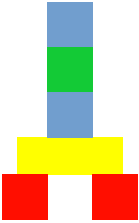
\includegraphics[scale=0.20]{figures/chapter2/task_goal.pdf}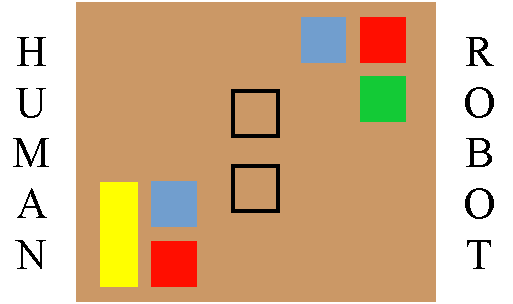
\includegraphics[scale=0.18]{figures/chapter2/task_setup_mini.pdf}}   
	\fancyhead[RO]{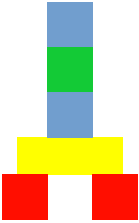
\includegraphics[scale=0.20]{figures/chapter2/task_goal.pdf}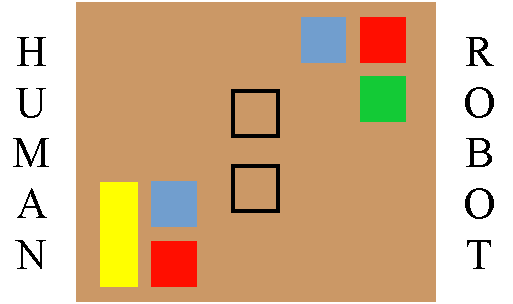
\includegraphics[scale=0.18]{figures/chapter2/task_setup_mini.pdf}\bfseries\thepage}  
	\fancyhead[RE]{\bfseries\nouppercase{\leftmark}}      % Chapter in the right on even pages
	\fancyhead[LO]{\bfseries\nouppercase{\rightmark}}     % Section in the left on odd pages
}%

\usepackage{pdfpages}
\usepackage{makecell}
\usepackage{pdflscape} 
\usepackage{mathtools}
\usepackage[section]{placeins}
\usepackage{afterpage}

%%%%%%%% my commands
\newcommand{\etal}{\textit{et al}.}
\newcommand{\ie}{\textit{i.e.}, }
\newcommand{\eg}{\textit{e.g.}, }
\newcommand{\fact}[3]{\mbox{\textit{#1}(#2, #3)}}
\newcommand{\circledtext}[1]{\raisebox{.5pt}{\textcircled{\raisebox{-.9pt} {#1}}}}
\newcommand{\sparql}{\textsc{SPARQL}}

\newcommand{\algConst}[1]{${\scriptscriptstyle #1}$}
\newcommand{\algNormTextSub}[2]{$\text{#1}_{#2}$}

\newcommand{\aslnumber}[1]{$#1$}
\newcommand{\aslstring}[1]{\textsf{#1}}
\newcommand{\aslvar}[1]{\textcolor{purple}{\textit{#1}}}
\newcommand{\asllabel}[1]{\textbf{#1}}
\newcommand{\annotation}[1]{{\footnotesize #1}}
\newcommand{\rulebody}[1]{\mbox{\hspace{.05\linewidth}}\begin{minipage}[t]{0.9\linewidth}#1.\end{minipage}}
\newcommand{\context}[1]{\begin{minipage}[t]{0.9\linewidth}#1\end{minipage}}
\newcommand{\planbody}[1]{\begin{minipage}[t]{0.9\linewidth}#1.\end{minipage}}
\newcommand{\Jason}[0]{\textbf{\textit{Jason}}}
\newcommand{\sn}{\mbox{\large\textbf{\texttt{\textasciitilde}}}}


\sloppy
\begin{document}
\fi


\chapter*{Introduction}
\addstarredchapter{Introduction} %Sinon cela n'apparait pas dans la table des matières
\markboth{INTRODUCTION}{}

Robots will interact more and more with humans in the future and thus will need to be endowed with the pertinent abilities. We are still far from having autonomous robots among humans and able to smoothly collaborate with them.

A lot of research focus on abilities needed to the robot to make it more intelligent, useful and adaptive: the planning, the perception, the knowledge management, the navigation, the action recognition, the dialog... But those does not make a robot function, those does not make a robot collaborate with a human in a task. What does? The supervision. Indeed, this component, such a puppeteer, controls from above the wires of the other architecture components. Leaning on them, it makes the decisions about how and when the robot should act, in a collaborative task with a human, it decides what the robot should say; reacting to the environment, the human behavior and the human speech. A robot should be able to act following a plan but more importantly, it should be able to react to the unexpected or to (robotic or human) errors. And what can give a robot such abilities? A supervision component, or we should say, a component with a vision.

Thereby, given the central role of this component, we could thought that it is extensively studied in \acrlong{hri}, a field of research whose aims is to build robots that will autonomously interact with humans. However, it is not. This lack led to a slight change of subject for this thesis. Indeed, initially, the goal was to devise a supervisor making the robot robust to a number of contingencies that could happen during a human-robot interaction. But, in order to have a supervisor handling contingencies, we needed first a supervisor for ``non-contingent'' situations. Well, we could not find any existing system implementing a supervision component in the context of human-robot collaborative tasks, on which we could build contingencies handling. Thus, we devised it.

\section*{A Supervision for \acrlong{hri}}
\markright{A Supervision for \acrlong{hri}}
When humans collaborate to achieve a task together, numerous neurocognitive mechanisms come into play, more than we would have thought at first glance. Some of these mechanisms are also triggered in humans’ minds when they interact with robots as they are essential to a successful collaboration. Therefore, it is important for roboticists designing robots that will closely interact with humans to be aware of and take into account the humans mental states and sensori-motor functions involved in controlling and smoothing collaborative task performance. However, this does not imply that robots have to be endowed with the same mechanisms since being able to collaborate with humans does not mean to imitate them. What is key to roboticists is to understand how humans work and to design  robots that will adapt. Consequently, we closely collaborated with a psychologist and a philosopher in order to learn the keys of human collaboration such as joint action, commitment, shared representations...(Chapter~\ref{chapter:chap1}) It was also back and forth discussions between them and us, trying to close the gap between what abilities a robot should have and what is currently technically possible.

Thus, when designing and implementing our supervisor for human-robot collaborative tasks, our minds were well nourished. In this thesis, we tackled the issue of a real component supervision for \acrshort{hri}. It endows the robot with a number of abilities in order to make the robot the best partner possible for humans such as modeling their mental states or adapting to their decisions (Chapter~\ref{chapter:chap5} and Chapter~\ref{chapter:chap6}).

\section*{A first step toward contingency handling}
\markright{A first step toward contingency handling}

Even though we could not lean on an existing supervision system in order to endow a robot with abilities making it able to cope with the unexpected, we started brainstorming on the subject. We realized that before being able to handle with contingencies, the robot should be able notice them. But, is it necessary to react immediately when something derails a bit or should there be a kind of threshold? As humans, sometimes, we run into minor incidents when performing a task for example, but as the situation is good overall, we tolerate it. Thus, we came with a novel idea: to give the robot the ability to evaluate, in real-time, the quality of its interaction with its human partner (Chapter~\ref{chapter:chap7}). This is a first step toward contingency handling as later, outside the scope of this thesis, it could integrated to the supervision, helping it to improve its decision and its reactions. For example, if something would go wrong during an action but the overall interaction quality was good, it could decide that it was not a matter of importance and ignore it. However, if it happened in the context of a bad quality or that the same action was going wrong again and again, then it could react.

\section*{Summary of the Thesis}
\markright{SUMMARY OF THE THESIS}

This manuscript is divided in four parts. 

The first part lays the funding principles of a decision-making system for human-robot collaboration. We start in Chapter~\ref{chapter:chap1} by providing a framework for reflecting upon key elements for human-human collaboration. We dive into psychology and philosophy literatures tackling multiple concepts, mainly around joint action such as shared representations, joint attention, coordination... But we also address social interactions, \acrlong{tom} and communication. 

Then, in Chapter~\ref{chapter:chap2}, we explore existing robotic systems implementing concepts associated to social interactions or joint action.

\bigskip 

The second part aims at presenting the key challenges of social interaction management. The supervision component belongs to a robotic architecture. Thus, in Chapter~\ref{chapter:chap3}, we present a number of robotic architectures and the one we integrated our component with. 

Then we highlight, in Chapter~\ref{chapter:chap4}, the central role of the supervision in this architecture as well as what tools are available to develop such a component and which one we chose.

\bigskip

In the third part are concentrated the two main contributions of this thesis: \acrfull{jahrvis}, the supervisor we devised, and a \acrfull{qoi} Evaluator. We start with an overview of the \acrshort{jahrvis} features in Chapter~\ref{chapter:chap5}, \ie a system embedding the robot high-level decisions, controlling its behavior, always considering the human it is interacting with. It is able to do so by taking into account shared plans, human mental states, its knowledge about the current state of the environment, and human actions, inspired by the principles described in Part~\ref{part:part1}. 

Then, we detail in Chapter~\ref{chapter:chap6}, one by one, the modules composing its structure: interaction management, human action recognition, shared plan handling, action execution management and communication management. It is accompanied with an example which has been executed on a PR2 robot. 

And, we introduce in Chapter~\ref{chapter:chap7}, a mean to evaluate from the robot point of view, the \acrlong{qoi}. We present the general concept, a set of metrics enabling such an ability and a way to aggregate these metrics. 

\bigskip

Finally, the fourth part present two tasks which have been executed thanks to the supervisor developed in the context of this thesis. The first task, presented in Chapter~\ref{chapter:chap8}, was tackled with the first version of \acrshort{jahrvis} in the context of a H2020 European project, \acrfull{mummer}\footnote{The \acrshort{mummer} project funded three years of this thesis out of four.}. The robot had to give directions to customers within a Finnish mall. This was a real challenge as the robot was deployed there for three months.

Lastly, in Chapter~\ref{chapter:chap9}, we present a task which was executed with the almost-complete version of \acrshort{jahrvis}. It is a task where a human and a robot partners have to communicate in order to remove the right cubes of a task. It was inspired by a task in psychology. We propose this task to the \acrshort{hri} community as a set of challenges to take up as well as a breeding ground for user studies.

\subsection*{List of Publications}
\markright{LIST OF PUBLICATIONS}
\subsubsection*{Published}
\begin{itemize}
\item Mayima, A., Clodic, A., \& Alami, R. (2021, August). Towards robots able to measure in real-time the Quality of Interaction. \textit{International Journal of Social Robotics.} 

\item Sarthou, G., Mayima, A., Buisan, G., Belhassein, K., \& Clodic, A. (2021, August). The Director Task: a Psychology-Inspired Task to Assess Cognitive and Interactive Robot Architectures. In \textit{2021 30th IEEE International Conference on Robot and Human Interactive Communication (RO-MAN)}.

\item  Mayima, A., Clodic, A., \& Alami, R. (2020, August). Toward a Robot Computing an Online Estimation of the Quality of its Interaction with its Human Partner. In \textit{2020 29th IEEE International Conference on Robot and Human Interactive Communication (RO-MAN)} (pp. 291-298).

\item Singamaneni, P-T., Mayima, A., Sarthou, G., Sallami, Y., Buisan, G., Y., Belhassein, K., Waldhart, J., \& Clodic, A. (2020, March). Guiding Task through Route Description in the MuMMER Project. [Video]. In \textit{HRI '20: ACM/IEEE International Conference on Human-Robot Interaction.} (pp.643-643).

\item Belhassein, K., Fernández Castro, V., \& Mayima, A. (2020). A Horizontal Approach to Communication for Human-Robot Joint Action: Towards Situated and Sustainable Robotics. In \textit{Culturally Sustainable Social Robotics}. (pp.204-214).

\item  Mayima, A., Clodic, A., \& Alami, R. (2019, November). Evaluation of the Quality of Interaction from the robot point of view in Human-Robot Interactions. In \textit{ The 11th International Conference on Social Robotics (ICSR) (1st Edition of Quality of Interaction in Socially Assistive Robots (QISAR) Workshop)}.
\end{itemize}

%\subsubsection*{Accepted}
%\begin{itemize}

%\end{itemize}
\subsubsection*{Submitted}
\begin{itemize}
\item Fernández Castro, V., Mayima, A., Belhassein, K., Clodic, A., The Role of Commitments in Socially Appropriate Robotics. Submitted in a volume of the Book \textit{Serie Techno:Phil}.

\item Mayima, A., Sarthou, G., Buisan, G., Singamaneni, P-T., Sallami, Y., Belhassein, K., Waldhart, J., Clodic, A., \& Alami, R. Direction-giving considered as a Human-Robot Joint
Action. Submitted to \textit{User Modeling and User-Adapted Interaction (UMUAI)}.

\item Belhassein, K., Fernández Castro, V., Mayima, A., Clodic, A., Pacherie, P., Guidetti, M., Alami, R, \& Cochet, H. Addressing joint action challenges in HRI: Insights from psychology
and philosophy. Submitted to \textit{Acta Psychologica}.
\end{itemize}	







 

\ifdefined\included
\else
\bibliographystyle{acm}
\bibliography{These}
\end{document}
\fi
\ifdefined\included
\else
\documentclass[a4paper,11pt,twoside]{StyleThese}
\usepackage{amsmath,amssymb, amsthm}             % AMS Math
\usepackage[T1]{fontenc}
\usepackage[utf8x]{inputenc}
\usepackage{babel}
\usepackage{datetime}

\usepackage{silence}

\WarningFilter{minitoc(hints)}{W0023}
\WarningFilter{minitoc(hints)}{W0028}
\WarningFilter{minitoc(hints)}{W0030}

\usepackage{lmodern}
\usepackage{tabularx}
%\usepackage{tabular}
\usepackage{multirow}
\usepackage{xspace}

\usepackage{subfig}
\usepackage[inline]{enumitem}

\usepackage{hhline}
\usepackage[left=1.5in,right=1.3in,top=1.1in,bottom=1.1in,includefoot,includehead,headheight=13.6pt]{geometry}
\renewcommand{\baselinestretch}{1.05}

% Table of contents for each chapter

\usepackage[nottoc, notlof, notlot]{tocbibind}
\usepackage{minitoc}
\setcounter{minitocdepth}{2}
\mtcindent=15pt
% Use \minitoc where to put a table of contents

\usepackage{aecompl}

% Glossary / list of abbreviations

\usepackage[intoc]{nomencl}
\iftoggle{ThesisInEnglish}{%
\renewcommand{\nomname}{Glossary}
}{ %
\renewcommand{\nomname}{Liste des Abréviations}
}

\usepackage{etoolbox}
\renewcommand\nomgroup[1]{%
  \item[\bfseries
  \ifstrequal{#1}{A}{Number Sets}{%
  \ifstrequal{#1}{G}{Agents Beliefs and Action Models}{%
  \ifstrequal{#1}{N}{Navigation}{%
  \ifstrequal{#1}{O}{Ontology}{%
  \ifstrequal{#1}{R}{Referring Expression Generation}{%
  \ifstrequal{#1}{Z}{Controllable and Uncontrollable Agents Task Planning}{}}}}}}%
]}

\makenomenclature



% My pdf code

\usepackage{ifpdf}

\ifpdf
  \usepackage[pdftex]{graphicx}
  \DeclareGraphicsExtensions{.jpg}
  \usepackage[pagebackref,hyperindex=true]{hyperref}
  \usepackage{tikz}
  \usetikzlibrary{arrows,shapes,calc}
\else
  \usepackage{graphicx}
  \DeclareGraphicsExtensions{.ps,.eps}
  \usepackage[dvipdfm,pagebackref,hyperindex=true]{hyperref}
\fi

\graphicspath{{.}{images/}}

%% nicer backref links. NOTE: The flag ThesisInEnglish is used to define the
% language in the back references. Read more about it in These.tex

\iftoggle{ThesisInEnglish}{%
\renewcommand*{\backref}[1]{}
\renewcommand*{\backrefalt}[4]{%
\ifcase #1 %
(Not cited.)%
\or
(Cited in page~#2.)%
\else
(Cited in pages~#2.)%
\fi}
\renewcommand*{\backrefsep}{, }
\renewcommand*{\backreftwosep}{ and~}
\renewcommand*{\backreflastsep}{ and~}
}{%
\renewcommand*{\backref}[1]{}
\renewcommand*{\backrefalt}[4]{%
\ifcase #1 %
(Non cité.)%
\or
(Cité en page~#2.)%
\else
(Cité en pages~#2.)%
\fi}
\renewcommand*{\backrefsep}{, }
\renewcommand*{\backreftwosep}{ et~}
\renewcommand*{\backreflastsep}{ et~}
}

% Links in pdf
\usepackage{color}
\definecolor{linkcol}{rgb}{0,0,0.4} 
\definecolor{citecol}{rgb}{0.5,0,0} 
\definecolor{linkcol}{rgb}{0,0,0} 
\definecolor{citecol}{rgb}{0,0,0}
% Change this to change the informations included in the pdf file

\hypersetup
{
bookmarksopen=true,
pdftitle="Endowing the robot with the abilities to control and evaluate its contribution to a human-robot joint action",
pdfauthor="Amandine MAYIMA", %auteur du document
pdfsubject="Thèse", %sujet du document
%pdftoolbar=false, %barre d'outils non visible
pdfmenubar=true, %barre de menu visible
pdfhighlight=/O, %effet d'un clic sur un lien hypertexte
colorlinks=true, %couleurs sur les liens hypertextes
pdfpagemode=None, %aucun mode de page
pdfpagelayout=SinglePage, %ouverture en simple page
pdffitwindow=true, %pages ouvertes entierement dans toute la fenetre
linkcolor=linkcol, %couleur des liens hypertextes internes
citecolor=citecol, %couleur des liens pour les citations
urlcolor=linkcol %couleur des liens pour les url
}

% definitions.
% -------------------

\setcounter{secnumdepth}{3}
\setcounter{tocdepth}{2}

% Some useful commands and shortcut for maths:  partial derivative and stuff

\newcommand{\pd}[2]{\frac{\partial #1}{\partial #2}}
\def\abs{\operatorname{abs}}
\def\argmax{\operatornamewithlimits{arg\,max}}
\def\argmin{\operatornamewithlimits{arg\,min}}
\def\diag{\operatorname{Diag}}
\newcommand{\eqRef}[1]{(\ref{#1})}

\usepackage{rotating}                    % Sideways of figures & tables
%\usepackage{bibunits}
%\usepackage[sectionbib]{chapterbib}          % Cross-reference package (Natural BiB)
%\usepackage{natbib}                  % Put References at the end of each chapter
                                         % Do not put 'sectionbib' option here.
                                         % Sectionbib option in 'natbib' will do.
\usepackage{fancyhdr}                    % Fancy Header and Footer

% \usepackage{txfonts}                     % Public Times New Roman text & math font
  
%%% Fancy Header %%%%%%%%%%%%%%%%%%%%%%%%%%%%%%%%%%%%%%%%%%%%%%%%%%%%%%%%%%%%%%%%%%
% Fancy Header Style Options

\pagestyle{fancy}                       % Sets fancy header and footer
\fancyfoot{}                            % Delete current footer settings

%\renewcommand{\chaptermark}[1]{         % Lower Case Chapter marker style
%  \markboth{\chaptername\ \thechapter.\ #1}}{}} %

%\renewcommand{\sectionmark}[1]{         % Lower case Section marker style
%  \markright{\thesection.\ #1}}         %

\fancyhead[LE,RO]{\bfseries\thepage}    % Page number (boldface) in left on even
% pages and right on odd pages
\fancyhead[RE]{\bfseries\nouppercase{\leftmark}}      % Chapter in the right on even pages
\fancyhead[LO]{\bfseries\nouppercase{\rightmark}}     % Section in the left on odd pages

\let\headruleORIG\headrule
\renewcommand{\headrule}{\color{black} \headruleORIG}
\renewcommand{\headrulewidth}{1.0pt}
\usepackage{colortbl}
\arrayrulecolor{black}

\fancypagestyle{plain}{
  \fancyhead{}
  \fancyfoot{}
  \renewcommand{\headrulewidth}{0pt}
}

%\usepackage{MyAlgorithm}
%\usepackage[noend]{MyAlgorithmic}
\usepackage{algorithm}
\usepackage[noend]{algpseudocode}
\usepackage{comment}
\usepackage[ED=MITT-InfoTel, Ets=INSA]{tlsflyleaf}
%%% Clear Header %%%%%%%%%%%%%%%%%%%%%%%%%%%%%%%%%%%%%%%%%%%%%%%%%%%%%%%%%%%%%%%%%%
% Clear Header Style on the Last Empty Odd pages
\makeatletter

\def\cleardoublepage{\clearpage\if@twoside \ifodd\c@page\else%
  \hbox{}%
  \thispagestyle{empty}%              % Empty header styles
  \newpage%
  \if@twocolumn\hbox{}\newpage\fi\fi\fi}

\newcommand*{\algrule}[1][\algorithmicindent]{%
	\makebox[#1][l]{%
		\hspace*{.2em}% <------------- This is where the rule starts from
		\vrule height .75\baselineskip depth .25\baselineskip
	}
}

%%% to have lines in algorithm, from stackexchange
\newcount\ALG@printindent@tempcnta
\def\ALG@printindent{%
	\ifnum \theALG@nested>0% is there anything to print
	\ifx\ALG@text\ALG@x@notext% is this an end group without any text?
	% do nothing
	\else
	\unskip
	% draw a rule for each indent level
	\ALG@printindent@tempcnta=1
	\loop
	\algrule[\csname ALG@ind@\the\ALG@printindent@tempcnta\endcsname]%
	\advance \ALG@printindent@tempcnta 1
	\ifnum \ALG@printindent@tempcnta<\numexpr\theALG@nested+1\relax
	\repeat
	\fi
	\fi
}
% the following line injects our new indent handling code in place of the default spacing
\patchcmd{\ALG@doentity}{\noindent\hskip\ALG@tlm}{\ALG@printindent}{}{\errmessage{failed to patch}}
\patchcmd{\ALG@doentity}{\item[]\nointerlineskip}{}{}{} % no spurious vertical space
% end vertical rule patch for algorithmicx

\makeatother
 
%%%%%%%%%%%%%%%%%%%%%%%%%%%%%%%%%%%%%%%%%%%%%%%%%%%%%%%%%%%%%%%%%%%%%%%%%%%%%%% 
% Prints your review date and 'Draft Version' (From Josullvn, CS, CMU)
\newcommand{\reviewtimetoday}[2]{\special{!userdict begin
    /bop-hook{gsave 20 710 translate 45 rotate 0.8 setgray
      /Times-Roman findfont 12 scalefont setfont 0 0   moveto (#1) show
      0 -12 moveto (#2) show grestore}def end}}
% You can turn on or off this option.
% \reviewtimetoday{\today}{Draft Version}
%%%%%%%%%%%%%%%%%%%%%%%%%%%%%%%%%%%%%%%%%%%%%%%%%%%%%%%%%%%%%%%%%%%%%%%%%%%%%%% 

\newenvironment{maxime}[1]
{
\vspace*{0cm}
\hfill
\begin{minipage}{0.5\textwidth}%
%\rule[0.5ex]{\textwidth}{0.1mm}\\%
\hrulefill $\:$ {\bf #1}\\
%\vspace*{-0.25cm}
\it 
}%
{%

\hrulefill
\vspace*{0.5cm}%
\end{minipage}
}

\let\minitocORIG\minitoc
\renewcommand{\minitoc}{\minitocORIG \vspace{1.5em}}

\usepackage{multirow}
%\usepackage{slashbox}

\newenvironment{bulletList}%
{ \begin{list}%
	{\tiny$\bullet$}%
	{\setlength{\labelwidth}{25pt}%
	 \setlength{\leftmargin}{30pt}%
	 \setlength{\itemsep}{-0.5em}}}%
{ \end{list} }

\newenvironment{inlineEnumerate}
{\begin{enumerate*} [label={(\arabic*)}] }
{\end{enumerate*}}

\theoremstyle{definition}
\newtheorem{definition}{Definition}
\renewcommand{\epsilon}{\varepsilon}

% centered page environment

\newenvironment{vcenterpage}
{\newpage\vspace*{\fill}\thispagestyle{empty}\renewcommand{\headrulewidth}{0pt}}
{\vspace*{\fill}}

\newenvironment{asl}{\ttfamily\begin{tabbing}~~~\=$\leftarrow$ \= ~~~ \=
		\kill}{\end{tabbing}}

\usepackage{tablefootnote}

\theoremstyle{plain}
\newtheorem{constraint}{Constraint}[section]

\algnewcommand\algorithmicforeach{\textbf{for each}}
\algnewcommand\algorithmicin{\textbf{in}}
\algdef{S}[FOR]{ForEach}[2]{\algorithmicforeach\ #1\ \algorithmicin\ #2\ \algorithmicdo}

\algnewcommand\algorithmicforkxor{\textbf{do fork-join-xor}}
\algnewcommand\algorithmicendforkxor{\textbf{end fork-join-xor}}
\algdef{SE}{ForkXor}{EndForkXor}{\algorithmicforkxor}{\algorithmicendforkxor}


\usepackage{listings}
\lstset{
	frame=single,
	captionpos=b,
	breaklines=true,
	basicstyle=\ttfamily,
	numberstyle=\color{black},
	tabsize=2,
	mathescape=true,
	literate=%
		{â}{{\^a}}1
}

\lstdefinestyle{inline}{
	frame=none,
	aboveskip=\smallskipamount,
	belowskip=\smallskipamount,
}

\lstdefinestyle{OwlTurtle}{
	language=C,
	tabsize=4,
	basicstyle=\scriptsize\ttfamily,
	keywordstyle=\bfseries\color{darkgray},
	morekeywords={rdf:type, rdfs:domain, rdfs:subPropertyOf, rdfs:range, :hasSubtask, :DecompositionUsedBy, rdfs:subClassOf, :hasDecomposition, owl:inverseOf, htn_actions:hasEffect, rdfs:label},
	alsoletter=:
}

\lstdefinestyle{aslDef}{
	frame=none,
%	breaklines=false,
	%xleftmargin=.1\textwidth, xrightmargin=.1\textwidth
}

\fancypagestyle{example}{%
	\fancyhead[LE]{\bfseries\thepage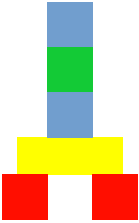
\includegraphics[scale=0.20]{figures/chapter2/task_goal.pdf}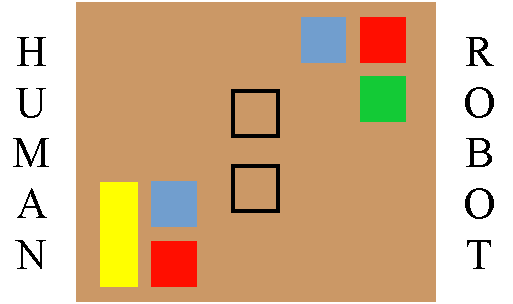
\includegraphics[scale=0.18]{figures/chapter2/task_setup_mini.pdf}}   
	\fancyhead[RO]{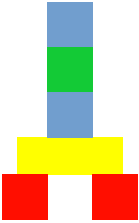
\includegraphics[scale=0.20]{figures/chapter2/task_goal.pdf}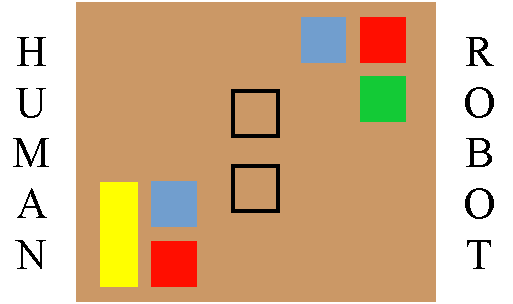
\includegraphics[scale=0.18]{figures/chapter2/task_setup_mini.pdf}\bfseries\thepage}  
	\fancyhead[RE]{\bfseries\nouppercase{\leftmark}}      % Chapter in the right on even pages
	\fancyhead[LO]{\bfseries\nouppercase{\rightmark}}     % Section in the left on odd pages
}%

\usepackage{pdfpages}
\usepackage{makecell}
\usepackage{pdflscape} 
\usepackage{mathtools}
\usepackage[section]{placeins}
\usepackage{afterpage}

%%%%%%%% my commands
\newcommand{\etal}{\textit{et al}.}
\newcommand{\ie}{\textit{i.e.}, }
\newcommand{\eg}{\textit{e.g.}, }
\newcommand{\fact}[3]{\mbox{\textit{#1}(#2, #3)}}
\newcommand{\circledtext}[1]{\raisebox{.5pt}{\textcircled{\raisebox{-.9pt} {#1}}}}
\newcommand{\sparql}{\textsc{SPARQL}}

\newcommand{\algConst}[1]{${\scriptscriptstyle #1}$}
\newcommand{\algNormTextSub}[2]{$\text{#1}_{#2}$}

\newcommand{\aslnumber}[1]{$#1$}
\newcommand{\aslstring}[1]{\textsf{#1}}
\newcommand{\aslvar}[1]{\textcolor{purple}{\textit{#1}}}
\newcommand{\asllabel}[1]{\textbf{#1}}
\newcommand{\annotation}[1]{{\footnotesize #1}}
\newcommand{\rulebody}[1]{\mbox{\hspace{.05\linewidth}}\begin{minipage}[t]{0.9\linewidth}#1.\end{minipage}}
\newcommand{\context}[1]{\begin{minipage}[t]{0.9\linewidth}#1\end{minipage}}
\newcommand{\planbody}[1]{\begin{minipage}[t]{0.9\linewidth}#1.\end{minipage}}
\newcommand{\Jason}[0]{\textbf{\textit{Jason}}}
\newcommand{\sn}{\mbox{\large\textbf{\texttt{\textasciitilde}}}}


\sloppy
\begin{document}
\setcounter{chapter}{0} %% Numéro du chapitre précédent ;)
\dominitoc
\faketableofcontents
\fi

\chapter{Human, Robot and Interaction Models: the Funding Principles of a Decision-Making System for Human-Robot Collaboration}
\label{chapter:chap1}
\chaptermark{Human, Robot and Interaction Models}
\minitoc

This first chapter aims at setting the context for this thesis. First, we present some related works on human-human and human-robot social interactions. These works nourished the thoughts which led to this manuscript. Then, we develop key elements for collaboration such as joint action, commitment and shared plans. Finally, we explore \acrfull{bdi} and cognitive robotic architectures  which have inspired us to design our own architecture in which, \acrshort{jahrvis} —  the main contribution of this thesis — endows a robot with the abilities not only to control, but also to evaluate its joint action with a human. 


\section{Social interactions}

\subsection{How to define a social interaction?}
First, let’s take a look at the dictionary and see how the word ``interaction'' is defined. According to the Oxford dictionary, an interaction is a ``reciprocal action or influence'' and more precisely a ``communication or direct involvement with someone or something''. As for the Cambridge dictionary, it defines it as an occasion when two or more people or things communicate with or react to each other''. Those definitions can give an hint about what it an interaction between humans but they are not specific enough. Now, going through social psychology literature, one of the first attempt to define ``social interaction'' can be found in~\cite{goffman_1967_interaction}. Goffman distinguishes three basic interaction units: the social occasion, the gathering and the social situation. The social occasion is an event that is temporally and spatially situated in such a way that it forms a unit that can be looked forward and back upon, by participants that are informed by the event (dinner, meeting, sport game...).  The gathering refers to any set of two or more individuals who are at the moment in one another’s immediate presence. It can be noted that a social occasion may include several gatherings but that gathering do not need social occasions to occur (they can happen in office spaces, street corners, restaurants…). The social situation refers to the full spatial environment that embraces interacting people. It is created as soon as people engage in interaction, when mutual monitoring occurs and ends when the next to the last person leaves. Furthermore, Goffman distinguishes between focused and unfocused interaction (gathering). A focused gathering has its members that can come together to sustain a joint focus of visual and cognitive attention and are open to each other for talk. He calls it encounters or engagements. On the other hand, an unfocused gathering has its members present to one another but not engaged together (e.g. persons waiting for a bus). In this same book, Goffman proposes a definition of social encounter: ``an occasion of face-to-face interaction, beginning when individuals recognize that they have moved into one another’s immediate presence and ending by an appreciated withdrawal from mutual participation''.

A couple of years later, Argyle wrote a book entitled Social Interaction~\cite{argyle_1973_social}, where he lay the foundations the basis to understand social interactions. He came to the view that social interaction could be interpreted as a set of social skills, and that it may therefore be possible to train those skills as manual skills are trained. For example, during an encounter between two persons, each must be able to perceive the social cues (verbal or non-verbal signals) of the other which are then filtered through the perspective each has acquired through socialization and experience.  The interpretation of context and social cues is then applied to arrive at a definition of the situation, which in turn guides both behavior and action.

Then, \cite{rummel_1976_understanding} proposes a definition of a few words: ``Social interactions are the acts, actions, or practices of two or more people mutually oriented towards each other's selves. It is behavior that tries to influence or take into account another's subjective experiences or intentions''.

Finally, the elements brought here, trying to define what is an interaction and more precisely a social interaction, are chosen among a large amount of work. It is possible to find different definitions, as \cite{enriquez_2017_vocabulaire} precises: ``although the term ``interaction'' is frequently used, it does not have a unique definition but presents semantic divergences''.

\subsection{Structure of a social interaction}
Most of the research about interaction and social interaction belongs to the field of social psychology. As for the structure of a social interaction, it is more from the field of Conversation Analysis (CA) which mixes sociology, anthropology, linguistics, speech-communication and psychology.
In~\cite{robinson_overall_2012}, Robinson makes a review of the work that has been done about ``overall structural organization''. Most of the time in the literature, overall structural organization is discussed in terms of ``the overall structural organization of entire, single occasions of interaction''.  Then ``overall structural organization'' term is generally used to talk about one particular (albeit large) unit of interaction. However, many different types of interactional units can have an overall structural organization. For example, in~\cite{schegloff_2011_word}, Schegloff encourages to recognize ``‘overall structural organization’ not as something for the unit ‘a single conversation’ (or encounter, or session, etc.) alone, but for units like turns, actions and courses of action (like answering or telling), sequences, and who knows what else as well.'' He also mentioned that every unit of organization should probably have a local organization and a global organization.
Here, the term ``overall structural organization'' is to refer to ``the overall structural organization of entire, single occasions of interaction''. Robinson tells us that this concept has received relatively little analytic attention and thus is still not well understood~\cite{robinson_overall_2012}. Indeed, research has been more focused on analyzing the organization of individual sequences of action such as turn-takings or conversation openings. Several terms have been used to talk about a ``supra-sequential coherence'': big package, set of pre-organized sequences, (social) activity, project of activity or plan of action. As the subject has not been investigated so much, it has not evolved a lot in 40 years, since what was proposed by Sacks~\cite{sacks_lectures_1995} to define overall structural organization of single occasions of interaction: it ``deals, roughly, with beginnings and endings, and how beginnings work to get from beginnings to something else, and how, from something else, endings are gotten to. And also the relationship - if there is one - between beginnings and endings''. Robinson summarizes research about the subject by saying that single occasions of interaction (in a generic or context-free sense) are normatively organized as: (1) beginning with an opening (2) ending with a closing and (3) having ``something'' in between opening and closing'' which can be referred to as topics.

\subsubsection{Opening}
Openings are used to begin an encounter. One of the main reference on the subject is~\cite{schegloff_1986_routine}. Openings and related issues vary depending on the nature of interactions. For example, opening of a phone call to a family member or a friend will be organized as follow: (1) summons-answer (the one calling talks first) (2) identification/recognition of each other (3) greetings and (4) how-are-you. Whereas, in primary-care medical visits, opening is sequenced as: (1) greeting (2) securing patients’ identities (2) retrieving and reviewing patients’ records and (4) embodying readiness (sitting down and facing one another). More examples from the literature can be found in (Robinson, 2012). 

Another work, \cite{kendon_1990_conducting}, focuses on the greeting part, but more precisely the greeting behavior with the associated non-verbal cues. The greeting behavior is divided in three main phases: the distance salutation, the approach and the close salutation. 
The distance salutation only occurs if the greeters as far enough such as they need to get closer if they wish to continue the interaction. This phase starts after one or both participants sight one another and at least one of them identifies a wish to engage in a greeting. In case one of the participant has not seen the other one, he signals his presence by vocalizing the other one’s name or by clearing his throat. Then, they orient their bodies towards each other and exchange glances in a subtle acknowledgement that the greeting is desired by both. During this phase, people can also wave or give a sign with their head (e.g. nod).
The approach is divided into two sub-phases: the distant approach (Kendon does not use this term) and the final approach. During the distant approach, people tend to look away whereas when the final approach starts (the greeters are 3 meters or less from one another), they look back at each other and, they smile.
Finally, there is the close salutation, the most normalized phase of the greeting. It happens when people are 1,5 meters or less from each others. Then, they can have a non-contact close salutation during which people exchange verbal greetings, or they can hand-shake or embrace (or do something else according to their culture). The greeting is over.
\subsubsection{Topics}
Episodes of interaction vary a lot in their contextualized nature, which leads to a large variety of topics and sequences of topics. Interactions that happen in ordinary or institutional contexts can be pre-organized around one or more topics. Robinson give examples such as an emergency call or an expected call back by a friend to discuss an expected single item of business.

\subsubsection{Closing}
One of the main reference to talk about closings is~\cite{schegloff_1973_opening}. A closing can be divided into two phases: the topic termination and the leave-taking.
The topic termination has a pre-closing statement which signals to the partner the wish to close the conversation. Then, the leave-taking follows the pre-closing statement and its response and, includes the goodbye exchange. Finally, the partners break co-presence, \ie, physically walk apart.\footnote{It is not explicitly mentioned in~\cite{schegloff_1973_opening}  but they precise in a footnote that it would not make sense if the parties remain in co-presence after having being through the closing sequence.} In the context of a phone call, Clark and French define this co-presence breaking as the \textit{contact termination} when people hang up.

With regards to non-verbal cues,  Knapp \etal lists and analyzes them~\cite{knapp_1973_rhetoric}. The more frequent are eye contact breaking,  head nodding, leaning toward the partner and positioning in the direction of the way of leaving.

\section{Human-Robot Social Interactions}

Now that we have seen how social interactions look like when happening between humans, we are going to see the different ways the human-robot interaction field divided and categorized interactions. 

\subsection{Short-term Interactions}
In~\cite{zheng_2013_designing}, they define a ``short-term interaction'' based on the Unified Theories of Cognition of Newell~\cite{newell_1994_unified}. A short-term interaction corresponds to the ``cognitive band'' of cognition, during which they focus on individual utterances and speech acts for interactions that last for tens of seconds. They leave aside longer-term interactions that can be in the ``rational band'' (minutes to hours) or the ``social band'' (days to months).
In~\cite{gaschler_2012_modelling}, their robot is a bartender then, they define a short-term interaction as being a customer ordering a drink – from the attention request towards the bartender to the closing of interaction by payment and exchange of polite phrases.
In~\cite{iocchi_2015_personalized}, they use ``short-term'' to refer to short interactions and that are focused on only one particular communicative objective, avoiding long and complex interactions.
In~\cite{sanelli_2017_short}, they give three characteristics to a short-term human-robot interaction: (1) users are not familiar with the robot (2) each interaction happens with a different user (3) interaction is short in time. Then the robot has not memory of past interactions.

\subsection{Long-term Interactions}
A survey~\cite{leite_2013_social} has been done about long-term human-robot interactions, where long-term means, most of the time, several interactions between the same human and robot. They defined four contexts for which social robot\footnote{actually, some of the robots featured in the survey are not social robots such as a Roomba or the Personal Exploration Rover (PER)} for long-term interaction have been designed: health care and therapy, education, work environment and public spaces, and people's homes. 
For example, Kanda \etal performed a field trial at an elementary school in Japan for two months~\cite{kanda_2007_two}. The children were able to interact with the robot for 32 days in total, during 30 minutes after lunch. The robot could switch between one hundred pre-defined behaviors (\eg hugging, shaking hand or singing) but not all of them were available during the first interactions with a human. Indeed, they had integrated a pseudo-development mechanism, \ie the more a child interacts with the robot, the more different behaviours the robot displays to that child. Also, the robot confided personal-themed matters to children who have often interacted with it (\eg ``I don't like the cold''). These abilities allowed the robot to maintain the children's interest even after the first week whereas in a first experiment where the robot's behavior was the same all along the two months, most children stopped to interact with the robot from the second week. 

In their discussion part, they raise an interesting question: How Long Should ``Long-Term'' Be? They found out that some authors consider that two months is a long-term interaction. They also point that some Human-Computer Interaction studies on long-term interaction last five weeks. Finally, the authors of the survey give their point of view, which seems well-thought. They argue that it is more important to look at the number of interaction sessions and the length of these sessions (a five minutes-interaction is different from a one hour-interaction). For them, an interaction can be considered as ``long-term'' when the user becomes familiarized with the robot to a point that their perception of such robot is not biased by the novelty effect anymore. This definition raises another question: when does user’s familiarization with the robot become stable? But it is not discussed here.

\subsection{Interactions divided in phases}
Gockley \etal ~\cite{gockley_2005_designing} invests the long-term human-robot interactions, i.e. over a long period of time, nine months. They divide an interaction is in three phases: greeting, core of the interaction and departure.In the greeting phase, Valerie, the robot receptionist, greets people who might be interested in engaging in conversation. To do so, people are classified into ``attentional'' states:
\begin{itemize}
	\item present (people a bit far and moving ) – Valerie doesn’t pay attention to them
	\item attending (people closer) – Valerie greets them
	\item  engages (people next to the desk but on the side) – Valerie acknowledges their presence but does not expect input from them
	\item interacting (people in front of the keyboard) – Valerie prompts them for input if they are not typing.
\end{itemize}

In the core of interaction, either Valerie can tell her (fictive) story or chat. Her story is subjective and evolve over time. It is about her social life, her lounge singing career, her therapy business, and her job as a receptionist. Furthermore, Valerie has a chatbot system which is very simple. Finally, inputs from visitors are from a keyboard, for easier control and reliability. Finally, at departure, when a person leaves the ``interacting'' region, Valerie signals the end of the interaction by saying ``goodbye.'' 

In~\cite{kidd_2008_robots}, they present a weigh loss coach. It introduces the notion of states of relationship. They are three: initial (for the first few days of interaction), normal, repair (if the result of Working Alliance Inventory – Short Form – questions asked by the robot – is less than -25). According to the state of relationship, the robot answers/questions/speech will not be the same.

In~\cite{kasap_2012_building}, to each user, corresponds an interaction session. Each session is composed of four dialogue phases: welcome, warm up, teach and farewell. The system has a memory of users and past interactions. In the memory, is recorded the context (initial state and goal), contents (events) and the outcome (goal succeeded or not).  A bit similar to the relationship state defined in~\cite{kidd_2008_robots}, they define a notion that they call relationship level. It is computed from the emotional interactions from the episodic memory associated to a user. It will influence the mood level and then the facial expression and the speech.

In~\cite{gaschler_2012_modelling}, they divide the interaction in three phases (or states) but from two different viewpoints, the of the customer and the one of the bartender. From the customer viewpoints, the phases are: (1) attention request towards bartender (2) ordering of one or more beverages, and (3) closing of interaction by payment and exchange of polite phrases. Then, in reaction of each phases, there are the ones from the bartender viewpoint: (1) acknowledging the attention request, (2) serving the ordered drink, and (3) asking for payment.
They leave open the possibility to have sub-phases inside phases.

We can also find in~\cite{lee_2012_personalization} the notion of structure of interaction: interactions start with the vendor identifying the customer, greeting and engaging in small talk with the customer, engaging in the snack transaction, and then enacting social leave-taking.
\subsection{Hierarchical interactions}
In~\cite{dautenhahn_2002_embodied} and~\cite{ogden_2001_interactional}, they define two levels of approach for interactions, a global one and a local one. Both papers are from the same authors but present some small differences in their definitions of the levels.
In~\cite{dautenhahn_2002_embodied}, the global level approach defines a unit of interaction as being relatively large, such as the script for a greeting as described by Kendon in~\cite{kendon_1990_conducting}. At this level, an interaction may be seen as a unit similar to a schema or script, in the computer/cognitive science senses of these terms. They name this level of interaction a global interactional unit, or GIU. Furthermore, a GIU can be divided in phases, each of which has associated behaviors. Behaviors have meaning and their meaning depends on the phase in which they occur, the context (e.g. a ‘wave hello’ vs. a ‘wave goodbye’). Finally, they discuss the advantages and drawbacks to describe an interaction at a global level. In~\cite{ogden_2001_interactional}, they prefer the use of the term ``long sequences of interaction'' rather than ``large units of interaction''.
In~\cite{dautenhahn_2002_embodied}, their local level approach is quite similar to the way CA views and analyzes interaction (e.g. adjacency pairs). This interactional structure is a much smaller unit, often as simple as an action and a response to that action. This view of interaction has the advantage of greater flexibility and robustness compared to the globally structured view. Flexibility is a result of the possibility of specifying acts that may occur in many global interactional structures. But, as contextual details are ignored, the ability to assign a specific meaning to an action is lost.

In his thesis~\cite{kuo_2012_designing}, Kuo insists about this flexibility and the re-usability. A lower level of design is more appropriate for reuse. For him, a unit of interaction corresponds to an ``interaction cue'' (or social cue) that a robot can perceive and act upon or express in an interaction. These cues can be verbal, non-verbal, or a combination of both (multi-modal interaction). A complete episode of interaction should be constructed through composition of interaction cues with some common patterns repeated over the course of the interaction (e.g. awareness of human presence).

\subsection{Patterns of Interaction}
Before talking about design patterns or interaction patterns, Goffman in 1983~\cite{goffman_1983_interaction} argues that human interactions follow a specific ``order'' and characterized a number of patterns in which people interact, such as how greetings unfold and how people leave an interaction.

In!\cite{kahn_2008_design}, they introduce design patterns, that they will later called interaction patterns in~\cite{kahn_2010_validating}, inspired from computer science. They propose rules to follow using them and eight patterns. The two main ideas to retain is that a sequence of patterns has to be well ordered and that patterns can be hierarchical. 
The 8 patterns: 
\begin{enumerate*}
	\item The initial introduction: largely scripted, conventionally-established verbal and behavioral repertoire to recognize the other, inquire politely about the other, engage in some physical acknowledgment (e.g. handshake)
	\item Didactic communication: one-way communication of information 
	\item In motion together: walk together
	\item Personal interests and history: sharing of personal interests and history with others
	\item Recovering from mistakes: creates the potential for both parties to maintain a social affiliation following the mistake
	\item Reciprocal turn-taking in game contextual: taking turns with one another when playing games
	\item Physical intimacy: to engage in holding or touching or embracing
	\item Claiming unfair treatment or wrongful harms: allows to make claim to its moral standing
\end{enumerate*}


Following the same idea and going further, Sauppé and Mutlu~\cite{sauppe_2014_design} introduces the interaction blocks. Compared to Kahn’s work, they offer a pattern language and a tool/environment to design human-robot interaction. To conceive their patterns, they collected and analyzed data from 5 kinds of interaction scenarios: Conversation, Collaboration, Instruction, Interview and Storytelling.
Then, they identified common interaction structures, which served as ``design interaction patterns'':
\begin{enumerate*}
	\item Introductory monologue: A short introduction can be used to introduce other participants to a scenario by giving an overview of the remainder of the interaction or it can be a greeting for example.
	\item Question and Answer: A question is a sentence meant to elicit information from other participants. An answer is the response to a question that aims to satisfy the questioning participant’s curiosity.
	\item Generic Comment and Personal Comment: A comment is a short statement offering the speaker’s opinion. Comments are either generic (e.g., ``Wow'') or personal (e.g., ``I tried that and didn’t like it'').
	\item Monologue and Generic Comment: A monologue is a longer form of speech during which no response is expected.(e.g. telling of a story). Although monologues expect no response, listeners may occasionally offer unsolicited commentary.
	\item Instruction and Action: An instruction is a command offered by one participant to direct the actions of another participant. The proper response to this instruction is often an action, although the action might follow the instruction with a delay depending on whether it is an appropriate time to perform that action
	\item Finished Comment: Upon the completion of the goals of the scenario, one or more of the participants will note that the scenario is completed by offering a finished comment.
	\item Wait: One pattern implicit in all scenarios involving two or more participants is the wait pattern.
\end{enumerate*}
Finally, they designed a software to easily implement those patterns in a robot.

In his thesis~\cite{kuo_2012_designing}, Kuo criticizes Kahn’s work. He says that these patterns involve sequences of interaction cues and should be decomposed to a lower level for detailed design and reuse. He proposes his own patterns:
\begin{enumerate*}
	\item Human presence detection: detect when there is a person who might be interested in
	\item Showing interest for interaction: express the robot’s awareness of a user’s presence around it and its interest and willingness to interact
	\item User’s attention on the robot: Know when a user is paying attention to the robot in an interaction and its information on its screen
	\item User identification by face: Provides the fundamental block for personal service and social interaction by recognising the human counterpart in an interaction
\end{enumerate*}
He checked the validity of his patterns with the analysis of Problem statement, Context of Use, Interaction Modality, Combination with Other Patterns, Technical Performance and Limitations, User Feedback and User’s Perception, Resulting Interactive Behavior.

Finally, Peltason and Wrede also based their work on design patterns from computer science, specifically applied to dialogue here~\cite{peltason_2010_pamini}. To name a few of them: Simple action request, Interaction opening, Interaction closing, Clarification. During interaction, the registered patterns are employed in a flexible way by admitting that patterns can be interrupted by other patterns and possibly resumed later which leads to interleaving patterns. By default, simpler patterns are permitted to be nested within temporally extended patterns.

\section{Context around the Joint Action Concept}


\subsection{Definitions of Joint Action and Examples of Robotic Implementations}
Often, multiple concepts are addressed when referring to collaborative tasks: collaboration, cooperation, coordination, joint action, joint activity, shared/joint attention, shared/joint intention, shared plan, shared/common/joint goal, (joint) commitment, engagement, mental states, theory of mind, mutual knowledge. However, many terms and definitions, whether inside a field or between fields do not reach a consensus.

\subsubsection{Human-Human Joint Action}
An important number of social interactions and encounters are encompassed by the notion of joint action. Broadly considered, joint action is any form of social interaction whereby two agents or more coordinate their actions in order to pursue a joint goal. However, the notion of joint action has been subject to debate in philosophy and psychology. For instance, according to Sebanz \etal~\cite{sebanz_2006_joint}, joint actions require the partners to coordinate ``their actions in space and time to bring about a change in the environment'' (p. 70); while other authors~\cite{carpenter_2009_just, cohen_1991_teamwork, fiebich_2013_joint, tomasello_2005_understanding} resist the idea that instances of mere coordination  – e.g. two partners walking side by side – constitute a joint action, considering that it requires some necessary conditions like sharing goals and intentions.

Moreover, while the notion of joint action is used interchangeably with the notion of collaboration or cooperation for some authors such as Becchio \etal~\cite{becchio_2010_toward} and Kobayashi \etal~\cite{kobayashi_2018_language}, other authors establish a hierarchy of interactions depending on the processes involved~\cite{amici_2015_coordination, chalmeau_1995_cooperation}. According to Amici and Bietti~\cite{amici_2015_coordination}, for example, coordination is a fast low-level process of behavioral matching and interactional synchrony which could, but not necessarily, facilitate middle-level processes like cooperation (where some individuals bear certain costs to provide benefits to others) or high-level processes like joint action, which requires other resources like turn-taking and alignment of linguistic resources during dialogue.

Leaving aside the debate on the concept of joint action, we aim to focus on the mechanisms that enable the consecution of joint actions. Three interrelated mechanisms appear to be key conditions for joint action: coordination, planning, and motivational alignment, each of them being supported by other processes. There has been an important deal of conceptual and empirical work investigating these processes~\cite{knoblich_2011_joint, pacherie_2012_agency}, from the sharing of a common ground to the anticipation of a partner’s actions by way of emergent coordination~\cite{curioni_2019_joint}. 

Most of all, joint actions require individuals to anchor their plans in the actual situation and generate particular coordinated actions~\cite{knoblich_2011_joint, vesper_2011_making}. This coordination can rely on different mechanisms, which are not necessarily intentional, including for example perception-action matching~\cite{brass_2001_movement}, perception of joint affordances~\cite{ramenzoni_2008_short}, joint attention~\cite{sebanz_2006_joint}. As for intentional coordination – sometimes referred to as planned coordination~\cite{curioni_2019_joint} –, it requires the partners: (i) to represent their own and others' actions, as well as the consequences of these actions, (ii) to represent the hierarchy of sub-goals and sub-tasks of the plan, (iii) to generate predictions of their joint actions, and (iv) to monitor the progress toward the joint goal in order to possibly compensate or help others to achieve their contributions~\cite{pacherie_2012_agency}.

Indeed, joint action often involves planning several aspects, which involves the representation of the goal and the whole plan, and/or even the sequence of actions to be performed. The formation of these types of representations could rely on different mechanisms, which include high-level processes such as theory of mind, team reasoning, or verbal negotiation~\cite{bratman_2013_shared} or more low-level processes as minimally representing the joint action goal and knowing that it will be achieved with others~\cite{vesper_2010_minimal}. An example of the mechanisms involved in planning a joint action is task co-representations, which allows individuals to represent the details of each other’s task. 

These representations allow individuals to generate predictions about the other’s actions, which in turn facilitate the adjustment and coordination between the partners. Interestingly, individuals can also facilitate the others’ and their own predictions by communicating relevant and reliable information for joint action. The objective is to make actions more transparent and predictable so that the decision-making on the interaction can be fluent and successful. Thus, participants in joint action often negotiate on the fly the sub-tasks, sub-goals, or ways to proceed regarding the collective task through different explicit exchanges~\cite{clark_1996_using}.



\subsubsection{Human-Robot Joint Action}\todo{part on emotions}


\subsection{Communication in Joint Action}

Cohen and Levesque, Teamwork, p 490

\subsection{Repairs in Joint Action}

One last subject of CA could be interesting for our problematic in human-robot interaction, it is the repair. It is a mean of correcting a misunderstanding or a mistake in an interaction, or of correcting a deviation from the normal rules of interaction. The ability to engage in repair is essential in interaction: errors and misunderstandings are likely to arise and must be corrected if the  goal of the interaction is to be successful. Generally, they are classified in four categories \cite{schegloff_1977_preference,wooffitt_2008_conversation}:
\begin{itemize}
	\item Self-initiated self-repair: Repair is both initiated and carried out by the responsible of the trouble
	\item Other-initiated self-repair: The responsible of the trouble takes care of the repair himself but the trouble have been pointed out by the other
	\item Self-initiated other-repair: The responsible of the trouble signals that a repair is needed and get the other one to repair (e.g. he forgot a name and asks for help to remember)
	\item Other-initiated other-repair: The one not responsible of the trouble initiates and carries out the repair. This is closest to what is conventionally understood as ``correction''.
\end{itemize}

\subsection{Commitments in Joint Action}


\section{Supervision systems for Decision and execution}

\subsection{BDI architectures}
There are several kind of integrated cognitive architectures, a survey describes the most known and representative of them~\cite{chong_2007_integrated}. Some of them have their roots in classical artificial intelligence as the Soar architecture. Others take their inspiration in cognitive psychology as ICARUS \todo{ref} which tries to produce artificial intelligence mimicking human cognition or the BDI architecture which is based on the studies of folk psychology and intentional systems. Furthermore, inspired by neurology, there is the subsumption architecture. It is a reactive architecture therefore, it is not based on symbolic mental representations but on sensory information fusion to select actions to execute. Finally, at the crossroads between AI, cognitive psychology and neurology, we can find the ACT-R\todo{ref} and CLARION\todo{ref} models.	
The BDI model is based on the philosophical model of human practical reasoning developed and designed by Michael Bratman~\cite{bratman_1987_intention,bratman_1988_plans}. It has 3 main concepts:
\begin{itemize}
	\item Beliefs: They are a representation of the agent’s knowledge about the world. ``[They] can be viewed as the informative component of system state''~\cite{rao_1995_bdi}. It is not the word ``knowledge'' that has been chosen to define this concept because what the agent perceives of the environment is in fact the likely state of the environment. There is no certainty, its sensors are not accurate or could malfunction. This way of distinguish knowledge and beliefs is one that can be found in the literature of distributed computing~\cite{lamarre_1994_knowledge}.
	\item Desires\footnote{In one of the first implementation, PRS, ``Goals'' notion was used instead of ``Desires''~\cite{georgeff_1989_decision}, then they use it in a interchangeable way in~\cite{georgeff_1991_modeling} and finally choose ``Desires''~\cite{rao_1995_bdi} with the definition given in the AI literature, \eg desires can be many at any instant and may be mutually incompatible. Therefore, a goal will be a chosen desire~\cite{cohen_1990_intention} and concurrent goals are consistent.}: They are a representation of the motivational state of the system. They provide ``information about the objectives to be accomplished or, more generally, what priorities or payoffs are associated with the various current objectives''~\cite{rao_1995_bdi}. 
	\item Intentions: They are a representation of the currently chosen course of action (plan). It is the deliberative component of the system. The selected course(s) of action are determined with a deliberative function, according to the beliefs and desires~\cite{rao_1995_bdi}.
\end{itemize}
\subsection{Supervision for Human-Robot Interactions}

\section{Limitations and Challenges}




\ifdefined\included
\else
\bibliographystyle{acm}
\bibliography{These}
\end{document}
\fi


\ifdefined\included
\else
\documentclass[a4paper,11pt,twoside]{StyleThese}
\usepackage{amsmath,amssymb, amsthm}             % AMS Math
\usepackage[T1]{fontenc}
\usepackage[utf8x]{inputenc}
\usepackage{babel}
\usepackage{datetime}

\usepackage{silence}

\WarningFilter{minitoc(hints)}{W0023}
\WarningFilter{minitoc(hints)}{W0028}
\WarningFilter{minitoc(hints)}{W0030}

\usepackage{lmodern}
\usepackage{tabularx}
%\usepackage{tabular}
\usepackage{multirow}
\usepackage{xspace}

\usepackage{subfig}
\usepackage[inline]{enumitem}

\usepackage{hhline}
\usepackage[left=1.5in,right=1.3in,top=1.1in,bottom=1.1in,includefoot,includehead,headheight=13.6pt]{geometry}
\renewcommand{\baselinestretch}{1.05}

% Table of contents for each chapter

\usepackage[nottoc, notlof, notlot]{tocbibind}
\usepackage{minitoc}
\setcounter{minitocdepth}{2}
\mtcindent=15pt
% Use \minitoc where to put a table of contents

\usepackage{aecompl}

% Glossary / list of abbreviations

\usepackage[intoc]{nomencl}
\iftoggle{ThesisInEnglish}{%
\renewcommand{\nomname}{Glossary}
}{ %
\renewcommand{\nomname}{Liste des Abréviations}
}

\usepackage{etoolbox}
\renewcommand\nomgroup[1]{%
  \item[\bfseries
  \ifstrequal{#1}{A}{Number Sets}{%
  \ifstrequal{#1}{G}{Agents Beliefs and Action Models}{%
  \ifstrequal{#1}{N}{Navigation}{%
  \ifstrequal{#1}{O}{Ontology}{%
  \ifstrequal{#1}{R}{Referring Expression Generation}{%
  \ifstrequal{#1}{Z}{Controllable and Uncontrollable Agents Task Planning}{}}}}}}%
]}

\makenomenclature



% My pdf code

\usepackage{ifpdf}

\ifpdf
  \usepackage[pdftex]{graphicx}
  \DeclareGraphicsExtensions{.jpg}
  \usepackage[pagebackref,hyperindex=true]{hyperref}
  \usepackage{tikz}
  \usetikzlibrary{arrows,shapes,calc}
\else
  \usepackage{graphicx}
  \DeclareGraphicsExtensions{.ps,.eps}
  \usepackage[dvipdfm,pagebackref,hyperindex=true]{hyperref}
\fi

\graphicspath{{.}{images/}}

%% nicer backref links. NOTE: The flag ThesisInEnglish is used to define the
% language in the back references. Read more about it in These.tex

\iftoggle{ThesisInEnglish}{%
\renewcommand*{\backref}[1]{}
\renewcommand*{\backrefalt}[4]{%
\ifcase #1 %
(Not cited.)%
\or
(Cited in page~#2.)%
\else
(Cited in pages~#2.)%
\fi}
\renewcommand*{\backrefsep}{, }
\renewcommand*{\backreftwosep}{ and~}
\renewcommand*{\backreflastsep}{ and~}
}{%
\renewcommand*{\backref}[1]{}
\renewcommand*{\backrefalt}[4]{%
\ifcase #1 %
(Non cité.)%
\or
(Cité en page~#2.)%
\else
(Cité en pages~#2.)%
\fi}
\renewcommand*{\backrefsep}{, }
\renewcommand*{\backreftwosep}{ et~}
\renewcommand*{\backreflastsep}{ et~}
}

% Links in pdf
\usepackage{color}
\definecolor{linkcol}{rgb}{0,0,0.4} 
\definecolor{citecol}{rgb}{0.5,0,0} 
\definecolor{linkcol}{rgb}{0,0,0} 
\definecolor{citecol}{rgb}{0,0,0}
% Change this to change the informations included in the pdf file

\hypersetup
{
bookmarksopen=true,
pdftitle="Endowing the robot with the abilities to control and evaluate its contribution to a human-robot joint action",
pdfauthor="Amandine MAYIMA", %auteur du document
pdfsubject="Thèse", %sujet du document
%pdftoolbar=false, %barre d'outils non visible
pdfmenubar=true, %barre de menu visible
pdfhighlight=/O, %effet d'un clic sur un lien hypertexte
colorlinks=true, %couleurs sur les liens hypertextes
pdfpagemode=None, %aucun mode de page
pdfpagelayout=SinglePage, %ouverture en simple page
pdffitwindow=true, %pages ouvertes entierement dans toute la fenetre
linkcolor=linkcol, %couleur des liens hypertextes internes
citecolor=citecol, %couleur des liens pour les citations
urlcolor=linkcol %couleur des liens pour les url
}

% definitions.
% -------------------

\setcounter{secnumdepth}{3}
\setcounter{tocdepth}{2}

% Some useful commands and shortcut for maths:  partial derivative and stuff

\newcommand{\pd}[2]{\frac{\partial #1}{\partial #2}}
\def\abs{\operatorname{abs}}
\def\argmax{\operatornamewithlimits{arg\,max}}
\def\argmin{\operatornamewithlimits{arg\,min}}
\def\diag{\operatorname{Diag}}
\newcommand{\eqRef}[1]{(\ref{#1})}

\usepackage{rotating}                    % Sideways of figures & tables
%\usepackage{bibunits}
%\usepackage[sectionbib]{chapterbib}          % Cross-reference package (Natural BiB)
%\usepackage{natbib}                  % Put References at the end of each chapter
                                         % Do not put 'sectionbib' option here.
                                         % Sectionbib option in 'natbib' will do.
\usepackage{fancyhdr}                    % Fancy Header and Footer

% \usepackage{txfonts}                     % Public Times New Roman text & math font
  
%%% Fancy Header %%%%%%%%%%%%%%%%%%%%%%%%%%%%%%%%%%%%%%%%%%%%%%%%%%%%%%%%%%%%%%%%%%
% Fancy Header Style Options

\pagestyle{fancy}                       % Sets fancy header and footer
\fancyfoot{}                            % Delete current footer settings

%\renewcommand{\chaptermark}[1]{         % Lower Case Chapter marker style
%  \markboth{\chaptername\ \thechapter.\ #1}}{}} %

%\renewcommand{\sectionmark}[1]{         % Lower case Section marker style
%  \markright{\thesection.\ #1}}         %

\fancyhead[LE,RO]{\bfseries\thepage}    % Page number (boldface) in left on even
% pages and right on odd pages
\fancyhead[RE]{\bfseries\nouppercase{\leftmark}}      % Chapter in the right on even pages
\fancyhead[LO]{\bfseries\nouppercase{\rightmark}}     % Section in the left on odd pages

\let\headruleORIG\headrule
\renewcommand{\headrule}{\color{black} \headruleORIG}
\renewcommand{\headrulewidth}{1.0pt}
\usepackage{colortbl}
\arrayrulecolor{black}

\fancypagestyle{plain}{
  \fancyhead{}
  \fancyfoot{}
  \renewcommand{\headrulewidth}{0pt}
}

%\usepackage{MyAlgorithm}
%\usepackage[noend]{MyAlgorithmic}
\usepackage{algorithm}
\usepackage[noend]{algpseudocode}
\usepackage{comment}
\usepackage[ED=MITT-InfoTel, Ets=INSA]{tlsflyleaf}
%%% Clear Header %%%%%%%%%%%%%%%%%%%%%%%%%%%%%%%%%%%%%%%%%%%%%%%%%%%%%%%%%%%%%%%%%%
% Clear Header Style on the Last Empty Odd pages
\makeatletter

\def\cleardoublepage{\clearpage\if@twoside \ifodd\c@page\else%
  \hbox{}%
  \thispagestyle{empty}%              % Empty header styles
  \newpage%
  \if@twocolumn\hbox{}\newpage\fi\fi\fi}

\newcommand*{\algrule}[1][\algorithmicindent]{%
	\makebox[#1][l]{%
		\hspace*{.2em}% <------------- This is where the rule starts from
		\vrule height .75\baselineskip depth .25\baselineskip
	}
}

%%% to have lines in algorithm, from stackexchange
\newcount\ALG@printindent@tempcnta
\def\ALG@printindent{%
	\ifnum \theALG@nested>0% is there anything to print
	\ifx\ALG@text\ALG@x@notext% is this an end group without any text?
	% do nothing
	\else
	\unskip
	% draw a rule for each indent level
	\ALG@printindent@tempcnta=1
	\loop
	\algrule[\csname ALG@ind@\the\ALG@printindent@tempcnta\endcsname]%
	\advance \ALG@printindent@tempcnta 1
	\ifnum \ALG@printindent@tempcnta<\numexpr\theALG@nested+1\relax
	\repeat
	\fi
	\fi
}
% the following line injects our new indent handling code in place of the default spacing
\patchcmd{\ALG@doentity}{\noindent\hskip\ALG@tlm}{\ALG@printindent}{}{\errmessage{failed to patch}}
\patchcmd{\ALG@doentity}{\item[]\nointerlineskip}{}{}{} % no spurious vertical space
% end vertical rule patch for algorithmicx

\makeatother
 
%%%%%%%%%%%%%%%%%%%%%%%%%%%%%%%%%%%%%%%%%%%%%%%%%%%%%%%%%%%%%%%%%%%%%%%%%%%%%%% 
% Prints your review date and 'Draft Version' (From Josullvn, CS, CMU)
\newcommand{\reviewtimetoday}[2]{\special{!userdict begin
    /bop-hook{gsave 20 710 translate 45 rotate 0.8 setgray
      /Times-Roman findfont 12 scalefont setfont 0 0   moveto (#1) show
      0 -12 moveto (#2) show grestore}def end}}
% You can turn on or off this option.
% \reviewtimetoday{\today}{Draft Version}
%%%%%%%%%%%%%%%%%%%%%%%%%%%%%%%%%%%%%%%%%%%%%%%%%%%%%%%%%%%%%%%%%%%%%%%%%%%%%%% 

\newenvironment{maxime}[1]
{
\vspace*{0cm}
\hfill
\begin{minipage}{0.5\textwidth}%
%\rule[0.5ex]{\textwidth}{0.1mm}\\%
\hrulefill $\:$ {\bf #1}\\
%\vspace*{-0.25cm}
\it 
}%
{%

\hrulefill
\vspace*{0.5cm}%
\end{minipage}
}

\let\minitocORIG\minitoc
\renewcommand{\minitoc}{\minitocORIG \vspace{1.5em}}

\usepackage{multirow}
%\usepackage{slashbox}

\newenvironment{bulletList}%
{ \begin{list}%
	{\tiny$\bullet$}%
	{\setlength{\labelwidth}{25pt}%
	 \setlength{\leftmargin}{30pt}%
	 \setlength{\itemsep}{-0.5em}}}%
{ \end{list} }

\newenvironment{inlineEnumerate}
{\begin{enumerate*} [label={(\arabic*)}] }
{\end{enumerate*}}

\theoremstyle{definition}
\newtheorem{definition}{Definition}
\renewcommand{\epsilon}{\varepsilon}

% centered page environment

\newenvironment{vcenterpage}
{\newpage\vspace*{\fill}\thispagestyle{empty}\renewcommand{\headrulewidth}{0pt}}
{\vspace*{\fill}}

\newenvironment{asl}{\ttfamily\begin{tabbing}~~~\=$\leftarrow$ \= ~~~ \=
		\kill}{\end{tabbing}}

\usepackage{tablefootnote}

\theoremstyle{plain}
\newtheorem{constraint}{Constraint}[section]

\algnewcommand\algorithmicforeach{\textbf{for each}}
\algnewcommand\algorithmicin{\textbf{in}}
\algdef{S}[FOR]{ForEach}[2]{\algorithmicforeach\ #1\ \algorithmicin\ #2\ \algorithmicdo}

\algnewcommand\algorithmicforkxor{\textbf{do fork-join-xor}}
\algnewcommand\algorithmicendforkxor{\textbf{end fork-join-xor}}
\algdef{SE}{ForkXor}{EndForkXor}{\algorithmicforkxor}{\algorithmicendforkxor}


\usepackage{listings}
\lstset{
	frame=single,
	captionpos=b,
	breaklines=true,
	basicstyle=\ttfamily,
	numberstyle=\color{black},
	tabsize=2,
	mathescape=true,
	literate=%
		{â}{{\^a}}1
}

\lstdefinestyle{inline}{
	frame=none,
	aboveskip=\smallskipamount,
	belowskip=\smallskipamount,
}

\lstdefinestyle{OwlTurtle}{
	language=C,
	tabsize=4,
	basicstyle=\scriptsize\ttfamily,
	keywordstyle=\bfseries\color{darkgray},
	morekeywords={rdf:type, rdfs:domain, rdfs:subPropertyOf, rdfs:range, :hasSubtask, :DecompositionUsedBy, rdfs:subClassOf, :hasDecomposition, owl:inverseOf, htn_actions:hasEffect, rdfs:label},
	alsoletter=:
}

\lstdefinestyle{aslDef}{
	frame=none,
%	breaklines=false,
	%xleftmargin=.1\textwidth, xrightmargin=.1\textwidth
}

\fancypagestyle{example}{%
	\fancyhead[LE]{\bfseries\thepage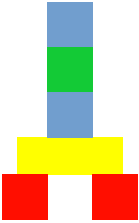
\includegraphics[scale=0.20]{figures/chapter2/task_goal.pdf}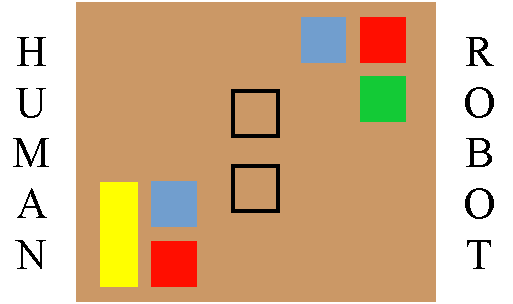
\includegraphics[scale=0.18]{figures/chapter2/task_setup_mini.pdf}}   
	\fancyhead[RO]{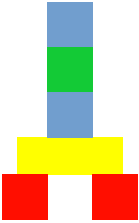
\includegraphics[scale=0.20]{figures/chapter2/task_goal.pdf}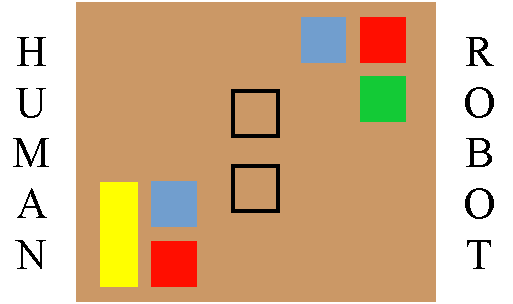
\includegraphics[scale=0.18]{figures/chapter2/task_setup_mini.pdf}\bfseries\thepage}  
	\fancyhead[RE]{\bfseries\nouppercase{\leftmark}}      % Chapter in the right on even pages
	\fancyhead[LO]{\bfseries\nouppercase{\rightmark}}     % Section in the left on odd pages
}%

\usepackage{pdfpages}
\usepackage{makecell}
\usepackage{pdflscape} 
\usepackage{mathtools}
\usepackage[section]{placeins}
\usepackage{afterpage}

%%%%%%%% my commands
\newcommand{\etal}{\textit{et al}.}
\newcommand{\ie}{\textit{i.e.}, }
\newcommand{\eg}{\textit{e.g.}, }
\newcommand{\fact}[3]{\mbox{\textit{#1}(#2, #3)}}
\newcommand{\circledtext}[1]{\raisebox{.5pt}{\textcircled{\raisebox{-.9pt} {#1}}}}
\newcommand{\sparql}{\textsc{SPARQL}}

\newcommand{\algConst}[1]{${\scriptscriptstyle #1}$}
\newcommand{\algNormTextSub}[2]{$\text{#1}_{#2}$}

\newcommand{\aslnumber}[1]{$#1$}
\newcommand{\aslstring}[1]{\textsf{#1}}
\newcommand{\aslvar}[1]{\textcolor{purple}{\textit{#1}}}
\newcommand{\asllabel}[1]{\textbf{#1}}
\newcommand{\annotation}[1]{{\footnotesize #1}}
\newcommand{\rulebody}[1]{\mbox{\hspace{.05\linewidth}}\begin{minipage}[t]{0.9\linewidth}#1.\end{minipage}}
\newcommand{\context}[1]{\begin{minipage}[t]{0.9\linewidth}#1\end{minipage}}
\newcommand{\planbody}[1]{\begin{minipage}[t]{0.9\linewidth}#1.\end{minipage}}
\newcommand{\Jason}[0]{\textbf{\textit{Jason}}}
\newcommand{\sn}{\mbox{\large\textbf{\texttt{\textasciitilde}}}}


\sloppy
\begin{document}
\setcounter{chapter}{1} %% Numéro du chapitre précédent ;)
\dominitoc
\faketableofcontents
\fi

\chapter{Joint-Action based Human-Aware supeRVISor: JAHRVIS}
\label{chapter:chap2}
\minitoc

\section{Introduction}

\section{Representation of a H-R collaborative activity}\label{sec:levels}
It is possible to describe and decompose a Human-Robot collaborative activity in various ways. For all the following definitions, we place ourselves in the context of one-to-one human-robot interactions, however we  believe that the scheme can be extended to multi-human multi-robot contexts. 
We draw our inspiration from the literature of sociology and robotics to define a model of interaction with three layered levels: interaction session, tasks and actions; as illustrated in Fig.~\ref{fig:levels}. We chose to represent collaborative tasks and their decomposition using the Hierarchical Task Network (HTN)~\cite{ghallab_2016_automated} representation which is often used in cognitive robotics~\cite{ingrand-2017,lallement_2014_hatp} and because it allows to deal with goal-based and situation-based activities at different levels of hierarchy such as task, subtasks and actions and consequently to consider different level of granularity. In the example of a task with an overall bad QoI, it would be interesting to know that in fact it is only a particular action or subtask ruining it. Indeed, the other parts of the task can be ok, or on the opposite, a particular subtask or action can have performed very well among the others. We need and use this granularity also on three levels defined (interaction session, tasks and actions) to finely evaluate the Quality of Interaction, as a task can be of poor quality but the session is globally going well. 

\begin{figure}[!ht]
	\centering
	\includegraphics[width=\linewidth]{figures/chapter2/session_interaction.pdf}
	\caption{The hierarchical structure of an interaction session. The highest level is the interaction session. The second level is composed of the tasks. They are included in the body of interaction of the interaction session and, two types of tasks are considered and may overlap, collaborative and conversational tasks. With this representation, a task can be recursively refined as subtasks until reaching the last level, the actions level, which is considered as atomic. Subtasks are not considered as a ``real'' level of the interaction session, specially to evaluate the QoI, as it may exist or not according to the task.
	}
	\label{fig:levels}
\end{figure}


\subsection{Representation of a H-R Interaction Session}
We define an \textbf{interaction session} as the period during which the robot and a human interact together and are engaged. It is divided in three parts, following the structure proposed by Robinson~\cite{robinson_overall_2012} and the engagement model of Sidner and Lee~\cite{sidner_2003_engagement}: the greetings, the body of the interaction and the goodbyes. First, \textit{the greetings} corresponds to the period where an agent starts an interaction by initiating it with another agent. The interaction session lasts as long as the interactants are maintaining the interaction through conversation and collaborative tasks performance which corresponds to the \textit{body of interaction}. Finally it ends when at least one of the interactants is disengaged, either by abruptly ending the interaction or by closing the interaction as described by Schegloff and Sacks~\cite{schegloff_1973_opening}, it corresponds to ``the goodbyes''. For example, for an entertainment robot in a mall, an \textit{interaction session} starts when a person signals to the robot that they want to engaged, by greeting it or by approaching it and looking at it. The body of interaction is composed of conversation and eventually direction-giving tasks and, the session lasts until the person says goodbye or leaves. This is the nominal case and, the duty of the robot is to contribute to maintain the session alive until the human decide to close it. However, in some (extreme) cases, the robot might decide to close the interaction by itself.

Social interactions and collaborative tasks involve engagement. There is no unique definition of what it means to be engaged. We chose one that is frequently used and has been proposed by Sidner and Lee~\cite{sidner_2003_engagement}: ``Engagement is the process by which two (or more) participants establish, maintain and end their perceived connection during interactions they jointly undertake''. The robot must be able to exhibit its engagement and disengagement and also to assess them with respect to its human partner.
We defined three states for the body of interaction, corresponding to what is happening during the latter: conversation (i.e. a social chit-chat or a goal negotiation, without any physical action performed except communicative gestures), collaborative task (i.e. both agents executing actions in order to achieve a shared goal) or idle phases (i.e. the agents are not chatting or performing a collaborative task together but remain engaged in the interaction session, it happens in-between active interaction phases). For each of these three states, the way to exhibit the engagement varies (e.g. in a conversation, an agent looking at their partner displays their engagement; during a task, an agent correctly performing their action is a way to demonstrate their engagement). That is why there is a need to define what behavior the robot has to exhibit in each state and what behavior it should expect from the human in each state, as these behaviors are usually very specific (e.g. in a direction-giving task, the robot keeps its head oriented toward its partner's face to demonstrate its engagement in conversation and idle contexts and when it gives a direction it expects the human to look at the direction it is showing; in a stack task, when the robot gives an instruction it expects the human to take a given cube).




\subsection{Collaborative Tasks, Substasks and Actions}
\textbf{\textit{Tasks}} compose the body of the interaction of an interaction session as shown in Fig.~\ref{fig:levels}. We distinguish conversation (i.e. agents engage in dialogue to exchange ideas, to ask questions, and to resolve differences) from collaborative tasks (i.e. agents work as partners, collaborating to perform tasks and to achieve common goals). We will not develop more on conversation since it is not the main focus of this paper, assessing the QoI of social dialog being another work.

In collaborative tasks, the robot and the human are committed to achieve a goal together, involving joint actions and shared plans~\cite{grosz_1996_collaborative}.  When a human and a robot perform a task together, as described by Bauer \textit{et al}.~\cite{bauer_2008_collab}, we could say that the robot has the intent to help the human, so the human's intention becomes its own intention. Then, they have the joint intention to reach a common goal and, as shown by Michael and Salice~\cite{michael_2017_commitment}, they have a commitment to the joint activity, leading to perform joint actions. Therefore, during its evaluation and decision-making processes, the robot has to take into account that the human and itself should remain engaged all along an interaction session for the tasks to be successful and both have to manage and contribute to maintain expectations about what the other is doing. 

The elements composing a \textit{task} are: a goal, a plan and involved agents. A plan is needed to realize a goal. There are many ways to generate a plan. But no matter the way (using a planner to anticipate execution or relying on a reactive planning scheme), a plan is a sequence of \textbf{\textit{subtasks}} which are sequences of actions -- \textit{subtasks} are not considered as a ``real'' level of the interaction session, specially to evaluate the QoI, as it may exist or not according to the task.
%-- sometimes it is not necessary to have an additional abstraction level, in this case a plan is directly composed of actions, with no subtasks. 

\textbf{\textit{Actions}} are the elementary items of tasks manipulated by the high-level robot supervision controller. They cannot be decomposed further by it (e.g. placement and motion planning are achieved by a lower control system not described here). It is usual to describe an action with its preconditions, its effects and, the agents and entities implied in its execution (e.g. in plans written in PDDL (Planning Domain Definition Language)~\cite{ghallab_98_pddl}). We add to this description the notion of expected reactions (which can themselves be actions) from the other agents once the action is executed.

In our model, an agent (human or robot) is a contributor to the task and has a mental state as described by Devin \textit{et al}.~\cite{devin_2016_implemented}. The mental state is a set of facts representing, from the agent point of view, the current world state, the state of the goal and the current task state. Since we are interested here by the robot situation assessment and decisional processes, the mental state of the human is built and managed by the robot as an estimation of the beliefs of the human~\cite{milliez_2014_framework, hiatt_2017_modeling,tabrez_2020}.

\subsection{Representation of a Human robot interaction session}

\subsection{Collaborative tasks, subtasks and actions}

\section{An example of architecture for robot autonomy dedicated to human robot interaction}\label{chap2:sec:rob_archi}

\subsection{Situation Assessment}

\subsection{Ontology}

\subsection{Task Planning}

\subsection{Motion Planning}

\subsection{Head Manager}

\subsection{Supervision}

\section{A robot controlling its contribution to a human-robot joint action}

\subsection{Introduction}

\subsection{Knowledge Management}

\subsection{Shared Plans Handling}

\subsection{Human Mental States Management}

\subsection{Action Monitoring}

\subsection{Communication}

\section{A robot evaluating its contribution to a human-robot joint action}\label{sec:qoi}

\subsection{Introduction}

Robots dedicated to Human-Robot interactions are not just machines receiving commands and executing them. They should be decisional agents with high-level goals, taking decisions (potentially taking into account social norms), and acting and reacting to not only their actions but those of other agents. Cognitive and interactive robots are becoming more and more capable thanks to the use of human-aware models and algorithms~\cite{kruse2013,thomaz_2016_computational}, with roboticists endowing them with the ability to execute their share of the work while adapting to contingencies, particularly those caused by human's behaviours and decisions~\cite{hoffman_2007_fluency,cakmak_2017,lemaignan-ai-2017}. The decision-making process is based on a range of knowledge about the environment, the interaction, the context... Nevertheless, curiously and interestingly, very little has been done to allow the robot, while performing its collaborative or assistive activity, to permanently evaluate if things are going well or not, as humans do. We name this ability ``the measure of the Quality of Interaction from the robot point of view''. We believe that enriching the robot knowledge with a good estimation about how the interaction is going, could enhance its decision-making process and thus, its social behaviour.

For example, if the robot detects that the QoI starts to drop, it can take a decision based on this information and act to try to improve the interaction quality (e.g. it can choose to change some modalities such as the language in which it communicates with the human, the volume of its speakers, or the parameters of its planners). On the contrary, when the QoI is high, the robot can decide to just continue the interaction as planned. Then, endowed with a QoI Evaluator, a robot becomes more adaptive and performs better. Also, a very poor performance all along a task could allow the robot to assess that the human is not really engaged in the interaction, or even is trying to play the robot. In such situation, the robot might perhaps better disengage. 
Finally, from a methodological point of view, a robot deployed in the wild able to assess interactions, has an asset compared to others as it could reduce the investment in material and human resources to perform user studies. And, a developer might use the logs to improve their design. 

In this paper, we only focus on the Quality of Interaction evaluation process and not on how to use its result for decision making. Therefore,  we present in the sequel the methods and tools we developed, allowing the robot to evaluate in real-time the quality of the human-robot collaborative activity it is involved in. It is based on a set of metrics we have defined, focused on two concepts: the measure of human engagement and the measure of the effectiveness of collaborative tasks performance. However, this is by no means exhaustive, and other metrics and parameters could (and should) be added later. Our work can be seen as a toolbox among which it is possible to pick the desired metrics according to tasks or contexts. We propose a way to aggregate these metrics, producing the QoI. The evaluation of the QoI is performed at three different levels of abstraction: the interaction session level, the task level and the action level. In further work, this ability could provide additional information to the robot and open the possibility for reconsidering its behaviour in case it estimates that the quality of the interaction is degrading (e.g. changing its plan or the way it is achieving it, informing the human or requesting a change in their behaviour, or even deciding to disengage).

The chapter is organized as follows. In the next section, we briefly discuss related work and the main challenges. In section~\ref{sec:levels} we present the representation of human-robot collaborative activity which we use and its hierarchical  decomposition. Finally, in sections \ref{sec:eval} and \ref{sec:metrics}, we introduce our concept and proposed set of metrics to evaluate the Quality of Interaction.

\subsection{Related work}\label{sec:rel}

Inspired from the evaluation methods used in Human-Computer Interactions and User Experience fields, the field of Human-Robot Interaction (HRI) has elaborated its own methods to evaluate robotic systems when they interact with humans. There are various ways to evaluate a human-robot interaction from the human perspective. Bethel \textit{et al}.~\cite{bethel_2010_review} divided them into five categories: \begin{enumerate*}[label={(\arabic*)}]
	\item self-assessments,\label{list:m_self}
	\item interviews,\label{list:m_inter}
	\item behavioral measures,\label{list:m_beha}
	\item psychophysiology measures, and\label{list:m_physio}
	\item task performance metrics\label{list:m_task}
\end{enumerate*}. They reviewed metrics used for each of the categories. They can be grouped into two types: \ref{list:m_self} and \ref{list:m_inter} are subjective metrics and, \ref{list:m_beha}, \ref{list:m_physio} and \ref{list:m_task} are objective ones. Since our aim is to have a robot able to evaluate interactions by itself, human subjective metrics are not usable. Then we focused on the study of existing objective metrics meant to measure how the interaction goes. Steinfeld \textit{et al}.~\cite{steinfeld_2006_common} proposed a set of metrics to be used in a wide range of tasks whose goal is to assess the system performance by measuring the task effectiveness (i.e., how well the task is completed) and the task efficiency (i.e., the time required to complete a task). Their work is very thorough and inspiring but does not target the evaluation of the quality of an on-going interaction. 
Hoffman~\cite{hoffman2019} defined a type of quality of interaction, the \textit{fluency}, pointing out that the notion is not well defined and somewhat vague but can still be assessed and recognized when compared to non-fluent scenario. To measure it, they propose a list of objective metrics, only based on duration measures, designed to be quite general: robot idle time, human idle time, concurrent activity (i.e., active time of both the robot and the human), functional delay (i.e., time difference between the end of one agent’s task and the beginning of the other agent’s task). It is an interesting way to measure the fluency and thus the quality of the human-robot interaction but it only applies to shared workspace tasks and is dedicated to an offline evaluation.

Systems targeting real-time measurements during human-robot interactions, with the purpose to ``close the loop'' and use the information for decision-making, have been developed. Tanevska \textit{et al}.~\cite{tanevska:hal-01615491} proposed a framework allowing the robot to perceive with face detection and evaluate in real-time the affective state (i.e. anger, happiness, sadness, surprise, etc) and the engagement state (i.e. whether the person is interested or bored in the interaction) of the people it is interacting with. However, the human affective state measure might not be enough to assess an interaction or a task as an affective state is actually a facial expression which can be misinterpreted (e.g. a smile can be a sign of happiness or embarrassment) and which might be not visible when one of the agent perform an action and looks somewhere else. Moreover, as the notion of engagement is very task specific, it needs further exploration. Real-time engagement measurement has also been investigated by Anzalone \textit{et al}.~\cite{anzalone_2015_evaluating} using metrics such as gaze, head pose, body pose and response times. Their work is interesting and could be an element among others to assess the interaction quality but, it is dedicated to face-to-face interactions. 

Cameras are not the only sensor used to assess interactions on-the-fly, some use human physiological responses such as skin conductance and temperature, heart or brain signals. Itoh \textit{et al}.~\cite{itoh2006}, Bekele \textit{et al}.~\cite{bekele_2014} or Kulic \textit{et al}.~\cite{kulic2007} use them to detect human affective states such as anxiety or liking in real-time. However, physiological measures often imply a lot of sensors which can be invasive for the human. And, as explained by Kulic and Croft~\cite{kulic_2003_estimating}, physiological signals may be difficult to interpret and there is a large variability in physiological response from person to person. Thus, it can be difficult for a controller to determine which emotional state the subject is in, or whether the response was caused by an action of the system, or by an external stimulus. Moreover, we claim that the human affective state only is not enough to assess the quality of an interaction, a human could be satisfied with an interaction or a task result even though they were stressed during it.

Finally,  Bensch \textit{et al}.~\cite{bensch17} proposed a formal approach to compute interaction quality in real-time. Their work focused on how to combine metrics together which is in the same line as ours. However, they do not provide implementation examples, remaining at an abstract level.

In summary, while a substantial number of studies have been devoted to the evaluation of collaborative interactions for analysis purposes once the interaction is over, there is a lack of methods allowing the robot to evaluate in real-time the quality of the interaction based on multiple metrics and not only anxiety or engagement. We claim that such an ability is very important and should strongly influence the situation assessment as well as the decisional abilities of interactive and collaborative robots. 




\subsection{The Quality of Interaction (QoI)}\label{sec:eval}

We believe the real-time assessment of the Quality of Interaction (QoI) with a human partner (i.e. what the robot ``thinks'' about how the interaction is going) is a new knowledge that could enhance the robot decision-making process. We define the Quality of Interaction as a measure that indicates how good is the interaction during human-robot collaborative activities. It is computed in real-time based on a set of metrics, at three different levels: the interaction session level, the tasks level and the actions level. The QoI of a given level is computed from selected metrics but also from the QoIs of the level below as shown in Fig.~\ref{fig:qoi_schema}.

\begin{figure}[!ht]
	\centering
	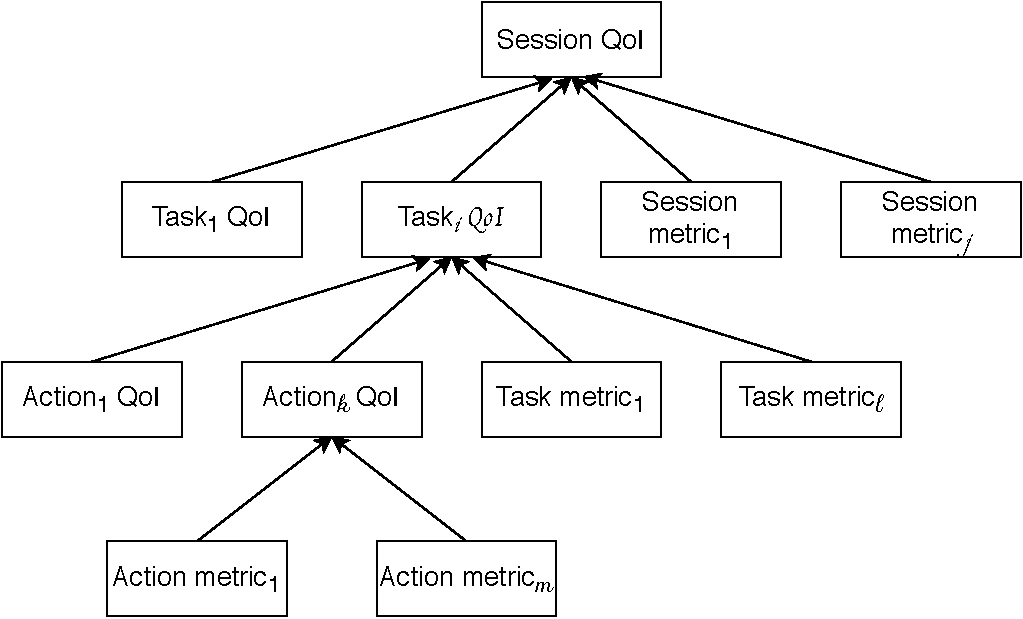
\includegraphics[width=\linewidth]{figures/chapter2/QoI_schema.pdf}
	\caption{Representation of the QoI dependencies, with $i$ the number of performed tasks during the interaction session, $k$ the number of performed actions during the task $i$, $j$ the number of metrics to measure the interaction session QoI, $l$ the number of metrics to measure the task $i$ QoI and $m$ the number of metrics to measure the action $k$ QoI.}
	\label{fig:qoi_schema}
\end{figure}

The QoI of each level is computed as a score between [($1$) for a good quality] and [($-1$) for a poor one]. Metrics used to compute the QoI are divided in three categories: 
\begin{itemize}
	\item $Mp \in [0,1]$ if it can only have a positive effect on the evaluation;
	\item $Mn \in [-1,0]$ if a metric can only have a negative effect on the evaluation;
	\item $M \in [-1,1]$ if a metric can have a positive or a negative effect.
\end{itemize}

Defined by the designer according to the needs and context, a metric can belong to one category or another depending on the target application. When needed, metrics values are scaled with the equations presented in Appendix~\ref{annex:functions}.

The evaluation of the Quality of Interaction at the level $l \in \{session_f,task_j,action_k\}$ (with $f,j \text{ and }k$ respectively the identifiers of a given interaction session, task and action),  $QoI_l$, is computed with:

\begin{equation}\label{eq:qoi}
QoI_{l}= \frac{ \sum\limits_{i=0}^x W_i * M_i}{\sum\limits_{i=0}^x W_i} + A * \frac{ \sum\limits_{i=0}^y Wn_i * Mn_i  + \sum\limits_{i=0}^z Wp_i * Mp_i}{\sum\limits_{i=0}^y Wn_i+\sum\limits_{i=0}^z Wp_i} 
\end{equation}


with $W_i, Wp_i,Wn_i$ respectively the corresponding designer-set weights of $M_i, Mp_i, Mn_i$, $A$ the designer-set weight of the right part of the $+$ sign and $x$, $y$, $z$ respectively the number of the metrics $M_i, Mp_i, Mn_i$.

Equation~\ref{eq:qoi} aggregates the values of the metrics chosen to be indicators of the interaction level quality. As all metrics do not have the same importance in the measure of the QoI, each of them is weighted. Values of these weights are empirically defined. There are two parts in the equation, the left part of the $+$ sign and the right part. The left part of the $+$ sign is a weighted mean of the third category of metrics, the $M$ metrics. The right part is a weighted mean of the metrics seen as bonus (i.e. $Mp$ metrics) or penalty (i.e. $Mn$ metrics). This latter part is weighted with $A$ -- whose value is also empirically\footnote{Values are empirically defined given intuition regarding the importance of a given metrics for a given task and a set of testing experiments} defined -- to be able to adjust its influence on the left part. In such a way, if there are no $Mn$ metrics to compensate for the $Mp$ metrics, it is possible to limit the positive influence of the $Mp$ metrics on the $M$ metrics with $A$. It is the same if there are no $Mp$ metrics, $A$ can compensate the impact of the $Mn$ metrics on the $M$ metrics. Even though $M, Mp, Mn \in [-1,1]$, the final result of $QoI_l$ might be less than $-1$ or greater than $1$ because of the addition of the $M$ with the $Mn$ and $Mp$. If it happens, $QoI_l$ minimal value is set to $-1$ and its maximal value is set to $1$.

\subsection{A set of metrics}\label{sec:metrics}

In this section, we present a few measures to assess the QoI of an interaction session in Sect.~\ref{subsec:m_intersess}. Then, we present metrics for the different levels based on engagement in Sect.~\ref{subsec:m_engag} and effectiveness estimations during human-robot joint activities in Sect.~\ref{subsec:task_eff}. For example, if the human is engaged and if tasks are performed effectively, the QoI will tend to be high and \textit{vice versa}. Both concepts are difficult to measure, so we do not exactly measure them but we compute their trends from the set of metrics presented in this section. This set is not exhaustive and will be extended in future work but it gave promising results as we show with our implementation in Chapter~\ref{chapter:chap3}. All metrics are meant to be used for online evaluations of interactions. They are summarized in Table~\ref{tab:theo_metrics}.

\begin{table*}[t]
	\centering
	\begin{tabular}{|c|p{0.5cm}|p{3cm}|p{3.5cm}|c||c|c|c|}
		\hline
		&  \multicolumn{2}{c|}{Metric names} & Measures & Illustration & Session & Task & Action \\
		\hline\hline
		\multirow{10}{*}{\rotatebox[origin=t]{90}{Effectiveness}} & \multirow{6}{*}
		{\rotatebox{90}{Progress towards goal}} & Distance-to-Goal  & Geometric distance & \parbox[c]{3.5cm}{
\includegraphics[width=3.5cm]{figures/chapter2/dtg.png}} & & x & x \\\cline{3-8}
		& & Time-to-Goal & Time & \parbox[c]{3.5cm}{
\includegraphics[width=3.5cm]{figures/chapter2/ttg.png}} & & x & x\\\cline{3-8}
		&  & Steps-to-Goal & Number of executed actions/substasks & \raisebox{-0.3cm}{\parbox[c][1.5cm]{3cm}{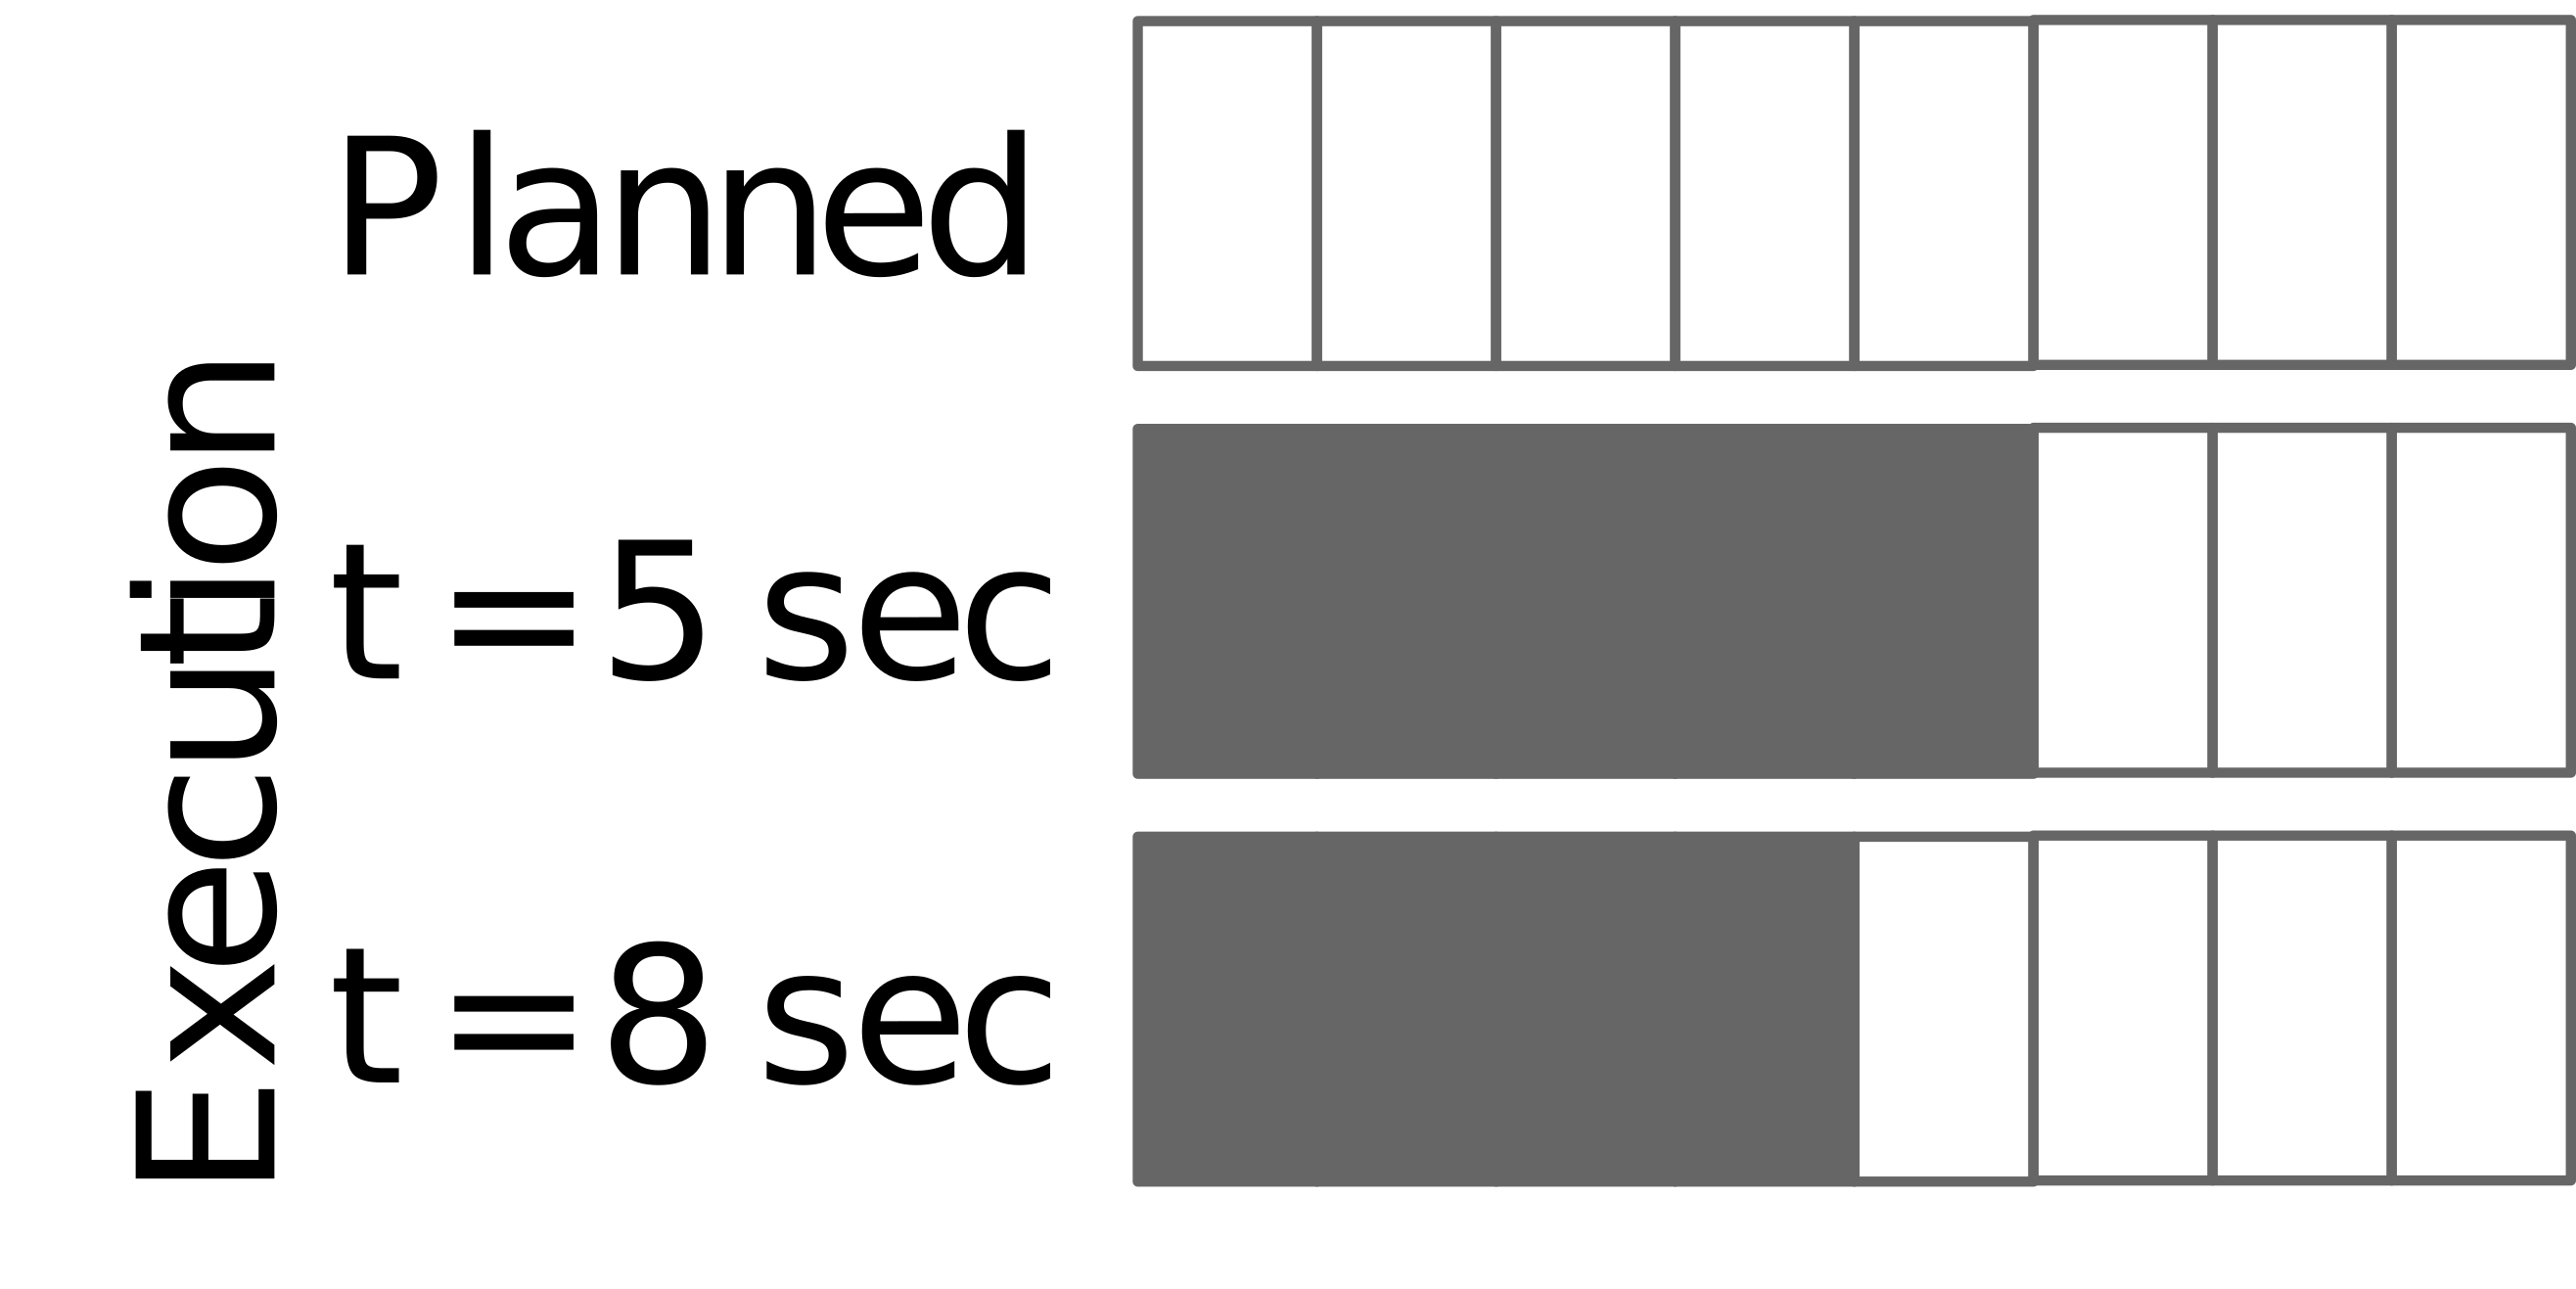
\includegraphics[width=3cm]{figures/chapter2/stg.png}}}&  & x &  \\\cline{2-8}
		&  \multicolumn{2}{p{3.5cm}|}{Deviation from standard duration} & Time & \parbox[c][1.2cm]{3.5cm}{
\includegraphics[width=3.5cm]{figures/chapter2/dd.png}}& & x & x \\\hline
		\multirow{5}{*}{\rotatebox[origin=c]{90}{Engagement}} 
		&  \multicolumn{2}{p{3.5cm}|}{Fulfilling robot expectations about social interaction} & e.g. attention ratio, with-me-ness,... & \raisebox{-0.6cm}{
\includegraphics[width=3.5cm]{figures/chapter2/ar.png}}&x & x & x \\\cline{2-8}
		&  \multicolumn{2}{p{3.5cm}|}{Human contribution to the goal} & e.g. number of repeated instructions, number of successful human actions,... & \raisebox{-0.8cm}{{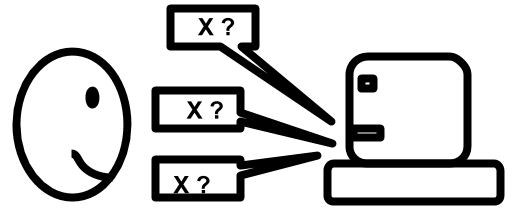
\includegraphics[width=2.4cm]{figures/chapter2/cg.png}}} & & x & x \\\hline
		% &  \multicolumn{2}{c|}{Interaction continuation} & e.g. duration, number of tasks/actions, termination manner & x & x & \\\hline
	\end{tabular}
	\caption{The set of metrics presented in Section~\ref{sec:metrics}.}
	\label{tab:theo_metrics}
\end{table*}     


\subsubsection{Measures to assess the QoI at the interaction session level}\label{subsec:m_intersess}
According to the context, the duration of an interaction session can be an indicator of the human engagement. Indeed, a human leaving only a few seconds after the beginning of the interaction is probably less engaged than a human staying with the robot several minutes. Also depending on the context, the number of executed tasks is a measure which can be considered as interesting information with respect to the engagement of the human, as well as the ratio of successful tasks. The more the human executes successful tasks with the robot, the higher the session QoI might be. Finally, it can be valuable to take into account how the session has been terminated in the evaluation of the quality of an interaction session. For instance, the fact that the human leaves abruptly in the middle of a task, during an idle time or a conversation without saying goodbye, or only at an appropriate time saying farewell to the robot is significant in terms of social interaction quality.

\subsubsection{Metrics related to human engagement}\label{subsec:m_engag}
Michael \textit{et al.}~\cite{michael2016} stated that commitments\footnote{In the robotic domain, it is the word ``engagement'' and not ``commitment'' which is often used, unlike in the psychological and philosophical fields.} facilitates ``the planning and coordination of joint actions involving multiple agents. Moreover, commitment also facilitates cooperation by making individuals willing to contribute to joint actions to which they would not be willing to contribute if they, and others, were not committed to doing so''. As it is an important element of the joint action, we want to provide the robot with a way to estimate the engagement of its partner during an interaction. 

Metrics allowing to state if an agent is engaged or not in an interaction are often specific to the type of interaction. For example, Fan \textit{et al.}~\cite{fan2017} implemented their measure of the human engagement as a kind of hysteresis: when the human gaze is on the robot, they are considered as engaged and when the human gaze is somewhere else during more than 3 consecutive seconds, they are considered as not-engaged. 

In the same vein, we think that the measure of the engagement for a collaborative activity can be divided in 2 types of metrics, summed up in Table~\ref{tab:theo_metrics}: the Human contribution to the goal and the Fulfilling robot expectations about social interaction.

We define in this section examples of metrics of each types which can be used to estimate the level of engagement of the human partner. 

\paragraph{Human contribution to the goal}\label{subsubsec:h_contrib}

A good and very promising indicator could be the ability from the robot to evaluate how well the human actions help to the goal progression. We call this indicator \textit{Human contribution to the goal}. To the best of our knowledge, there is no general method to estimate it. 

As a first version of the \textit{Human contribution to the goal}, we chose to measure it through the number of times the robot has to repeat an instruction or a question before the human performs correctly, when it expects the human to answer or to perform the action. As, if it needs to repeat, it means that the human is not correctly contributing to the goal, intentionally or not, as they are not performing their part of the HR action as they should. The more the robot needs to repeat because of the human's bad performance, the less they are contributing to the goal, the more the action QoI should decrease. 

\paragraph{Fulfilling robot expectations about social interaction}\label{subsubsec:r_exp}
During a social interaction, agents are expected to behave in a certain way and so the robot has expectations about the human. Then, the robot can monitor the human behavior to check if they are acting as they are expected to. For example, most of the time, when the robot speaks to the human, it will expect them to look at it and so it can monitor if it is the case or not as implemented by Fan \textit{et al.}~\cite{fan2017}. Quite similarly, Lemaignan \textit{et al.}~\cite{lemaignan2016} developed a way to measure if the human is \textit{with} the robot during their interaction, based on attention assessment, by computing if the human is looking at the desired attentional target or not. This latter metric will be integrated to our framework in future work.

As the works of Lemaignan \textit{et al.} and Fan \textit{et al.}, we estimate the \textit{Fulfilling robot expectations about social interaction} with the human head orientation, in the context of our implementation described in Chapter~\ref{chapter:chap3}. We compute an attention ratio i.e., the time during which the human is attentive to the robot (i.e. staying close enough and looking at it) when it speaks compared to the total time of the speech:

\begin{equation}\label{eq:attention_r}
Ar = \frac{duration_{isAttentiveTo(robot)=true}}{duration_{robot\_speaks}}
\end{equation}

\paragraph{Metrics related to effectiveness}\label{subsec:task_eff}
One can elaborate metrics to measure how well a task or an action is achieved. As discussed by Olsen and Goodrich~\cite{olsen_2003_metrics}, there are a variety of metrics such as time-based metrics which reward the speed of performance or the response times; error metrics which are based on counting retrials, failures, or mistakes; coverage metrics which measure to what extent a goal is achieved, as well as other possible metrics. We use some of them such as counting retrials, however these metrics alone were not enough for our example task as we are in a HRI context.

One can measure for different kinds of tasks, the ratio of successful\footnote{Obviously, the success is context and task dependent and should be defined according to the needs} executions to the total number of executions (e.g. $R=\dfrac{Succ}{Exec}$) or the deviation from the initial plan (distance, cost, trajectory, etc). 

We define four metrics, summed up in Table~\ref{tab:theo_metrics}, allowing to measure the current task and action effectiveness. Three of them are means to measure how the progress towards the goal of a task or an action varies. Indeed, they are good indicators for the interaction quality as, when executing a task or an action, if the agents are not getting closer from the goal or even diverged from it, it means that something goes wrong. There are three different metrics because the one to use depends on the type of task or action. The fourth metric allows to compare the current execution duration to the standard execution duration of the task or action, based on durations measured during previous executions.

\paragraph{Metrics to assess the progress towards the goal}

We defined three different metrics to assess the progress towards the goal. The first one allows to assess the progress towards the goal of geometric-based actions. The second estimates the progress by using the remaining time to reach the goal. Finally, the last one measures the number of remaining steps (actions or substasks) before achieving the goal of a task.

\subparagraph{Distance-to-Goal}\label{para:dtg_gd} 
When an agent is performing a geometric-based action such as a movement, observing if the agent is getting closer to the target position over time provides a useful information about how well the action is going. Therefore, we introduce the \textit{Distance-to-Goal} $\Delta DtG$ metric: 
\begin{equation}\label{eq:dtgg}
\left\{
\begin{array}{ll}
\Delta DtG(t=0) = 0\\
\begin{aligned}
\Delta DtG(t) &= \max(0,\Delta DtG(t-1) - 1)  \\&\text{if } path\_length(t) <  path\_length(t-1) \\

\end{aligned}\\
\Delta DtG(t)= \Delta DtG(t-1) + 1, \text{otherwise.}

\end{array}
\right.
\end{equation}
with $path\_length(t)$ the length of the path leading the goal at time $t$ (e.g. which can be given by a reactive motion planner~\cite{khamb2019}). The metric lower bound is 0. If at time $t$ the agent is closer to its final position than at $t-1$, i.e. progressing towards their goal, the metric is set to decrease or to remain equal to 0. Now, if the agent has not moved or is even further, the metric increases. The closer the metric value is to 0, the better it is, as it means the distance to the goal has decreased over time. We chose to not directly compute the difference between  $path\_length(t)$ and  $path\_length(t-1)$ as the results would be very different whether it is an action implying a long path or a short path. 

\subparagraph{Time-to-Goal}\label{para:dtg_t}
This measure is intended to estimate the progress of a given task or action towards its goal based on the estimation of the remaining time to reach it. It compares the current estimated time to goal with the initial estimated time to goal taking into account the current task duration. As so, it is possible to measure the variation compared to the initial plan. We define the \textit{Time-to-Goal} $\Delta TtG$ as:
\begin{equation}\label{eq:ttg}
\Delta TtG(t) = \max(0, e(t)  + TtG(t) - TtG(T_0))
\end{equation}
with $e(t) = t - T_0$ the task execution duration (time elapsed since the beginning of the task), $TtG(t)$ the current time to the goal, and $TtG(T_0)$ the initial planned time to goal. In our work, $TtG(t)$ and $TtG(T_0)$ are provided by a reactive motion planner~\cite{khamb2019} because we used the metric for navigation but it could be provided by other kind of planners. 

\begin{figure}[!htb]
	\centering
	% Maximum length
	\subfloat[Plot of $\phi(t)_{X}$ of the subtask $X$ lasting 60 seconds, with $SD_{X}=10 sec$, $V_{X}=0.5$ and $\alpha=1$]{\label{fig:oteX}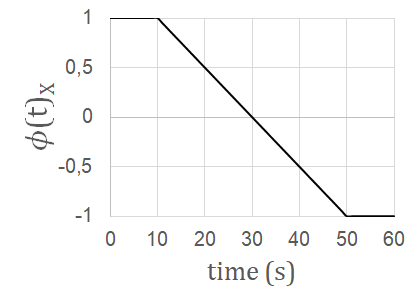
\includegraphics[width=0.49\linewidth]{figures/chapter2/oteX_2.png}}\hfill
	\subfloat[Plot of $\phi(t)_{Y}$ of the subtask $Y$ lasting 15 seconds, with $SD_{Y}=5 sec$, $V_{Y}=1$ and $\alpha=0.5$]{\label{fig:oteY}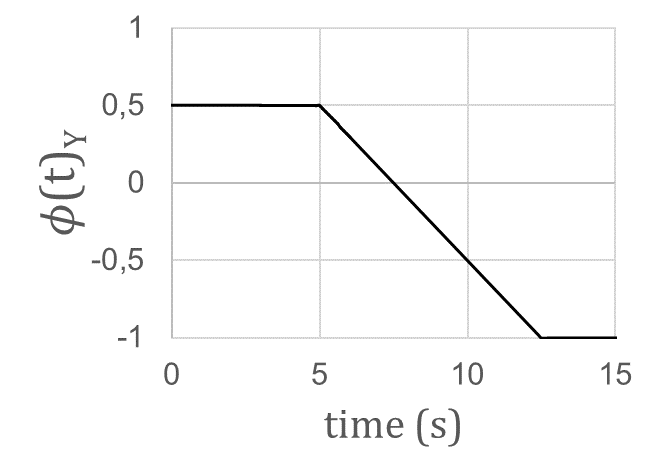
\includegraphics[width=0.49\linewidth]{figures/chapter2/oteY_2.png}}\hfill
	\subfloat[Plot of $\Phi(t)_{Ta}$ for a task composed of a sequence of three subtasks $X, Y, Z$: the duration of $X$ exceeded $SD_X=10 s$ and reached $20 s$, the duration of $Y$ exceeded $SD_Y= 5s$ and reached $10 s$, finally the duration of $Z$ was less than $SD_Z=10s$]{\label{fig:ote2}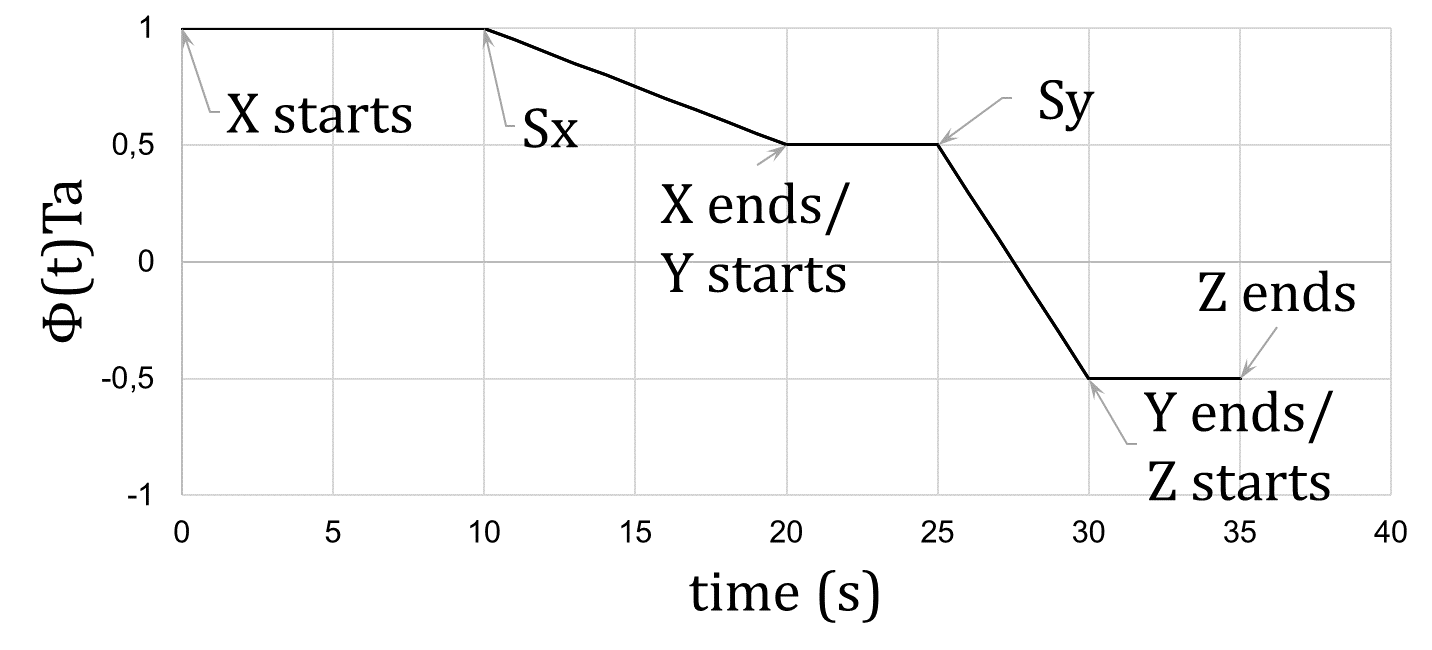
\includegraphics[width=0.7\linewidth]{figures/chapter2/ote.png}}\hfill
	\caption{Examples of plots of the $\phi$ and $\Phi$ functions}
	\label{fig:ote}
\end{figure}

\subparagraph{Steps-to-Goal}
One way to estimate the remaining distance to the goal for a task is to count the number of remaining substasks or actions (depending on the relevant scale) to perform. In addition, one can add a factor which estimates the weight (or effort needed) of each action or subtask. These weights can be determined by the designer, provided by the planner, etc. 
Then, the \textit{Steps-to-Goal} $\mathcal{D}$  of a task can be computed as time $t$:
\begin{equation}\label{eq:edtgs}
\mathcal{D}(t) = \dfrac{\sum\limits_{i=1}^c \mathcal{W}_i}{\sum\limits_{i=1}^n \mathcal{W}_i}
\end{equation}
with $\mathcal{W}_i$ the weight of a subtask/action $i$, $c$ the number of completed subtasks/actions and $n$ the total number of planned subtasks/actions.

\paragraph{Deviation from standard duration}\label{subsubsec:ote}
We introduce here a metric to measure the deviation from standard execution duration, the \textit{Deviation from standard duration} $\phi$ for subtasks/actions and the \textit{Deviation from standard duration} $\Phi$ for a whole task. This measure is intended to represent the degradation of the quality of execution of a HR task when its duration exceeds a certain time. 

To each subtask/action $a_i$, we associate two attributes whose values are defined by the designer: a soft deadline $SD_i$ and a decreasing quality  speed $V_i$. 
If, at time $t$, the execution duration  $e(t) = t - T_0$ of a substask or action $a_i$ which has started at $T_0$ exceeds $SD_i$, the quality will decrease over time at speed $V_i$: 
\begin{equation}\label{eq:ote}
\phi(t)_i=\max\left( V_i*\frac{-\max(e(t)-SD_i,0)}{SD_i}+\alpha,-1\right)
\end{equation}
where $\alpha$ is the value initial value and the upper bound (as at $t=0$, $\max(e(t)-SD_i,0)=0$) of $\phi_i$, when the subtask/action $a_i$ starts.

Then, we define a metric $\Phi$ for a task. It is an aggregation of the $\phi_i$ computed for each performed subtask/action $a_i$ of the task. At any moment, $\Phi$ can be seen as a memory of the previous steps, so the initial value $\alpha$ of $a_i$ is equal to the final value of $\phi_{i-1}$ of the previous subtask/action $a_{i-1}$, $\alpha=\phi(T_{final})_{i-1}$.


We can notice that it is not possible for this metric to increase over time since it memorizes the values of the previous actions. However, the total computed QoI can get higher thanks to the other metrics. Moreover, $\phi$ can be used independently of $\Phi$. In such a case, the initial of value $\alpha$ of $\phi$ can be set to 1. 

Three examples are given in Fig.~\ref{fig:ote}. Fig.~\ref{fig:oteX}~and~\ref{fig:oteY} represent $\phi(t)_{X}$ and $\phi(t)_{Y}$ for two independent subtasks $X$ and $Y$. Fig.~\ref{fig:ote2} is a plot of $\Phi(t)_{Ta}$ for the task $Ta$ composed of the subtasks $X, Y, Z$ with $SD_X=10 s$, $V_X=0.5$, $SD_Y=5 s$, $V_Y=1$, $SD_Z=10 s$ and $V_Z=1$. 

\ifdefined\included
\else
\bibliographystyle{acm}
\bibliography{These}
\end{document}
\fi

\ifdefined\included
\else
\documentclass[a4paper,11pt,twoside]{StyleThese}
\usepackage{amsmath,amssymb, amsthm}             % AMS Math
\usepackage[T1]{fontenc}
\usepackage[utf8x]{inputenc}
\usepackage{babel}
\usepackage{datetime}

\usepackage{silence}

\WarningFilter{minitoc(hints)}{W0023}
\WarningFilter{minitoc(hints)}{W0028}
\WarningFilter{minitoc(hints)}{W0030}

\usepackage{lmodern}
\usepackage{tabularx}
%\usepackage{tabular}
\usepackage{multirow}
\usepackage{xspace}

\usepackage{subfig}
\usepackage[inline]{enumitem}

\usepackage{hhline}
\usepackage[left=1.5in,right=1.3in,top=1.1in,bottom=1.1in,includefoot,includehead,headheight=13.6pt]{geometry}
\renewcommand{\baselinestretch}{1.05}

% Table of contents for each chapter

\usepackage[nottoc, notlof, notlot]{tocbibind}
\usepackage{minitoc}
\setcounter{minitocdepth}{2}
\mtcindent=15pt
% Use \minitoc where to put a table of contents

\usepackage{aecompl}

% Glossary / list of abbreviations

\usepackage[intoc]{nomencl}
\iftoggle{ThesisInEnglish}{%
\renewcommand{\nomname}{Glossary}
}{ %
\renewcommand{\nomname}{Liste des Abréviations}
}

\usepackage{etoolbox}
\renewcommand\nomgroup[1]{%
  \item[\bfseries
  \ifstrequal{#1}{A}{Number Sets}{%
  \ifstrequal{#1}{G}{Agents Beliefs and Action Models}{%
  \ifstrequal{#1}{N}{Navigation}{%
  \ifstrequal{#1}{O}{Ontology}{%
  \ifstrequal{#1}{R}{Referring Expression Generation}{%
  \ifstrequal{#1}{Z}{Controllable and Uncontrollable Agents Task Planning}{}}}}}}%
]}

\makenomenclature



% My pdf code

\usepackage{ifpdf}

\ifpdf
  \usepackage[pdftex]{graphicx}
  \DeclareGraphicsExtensions{.jpg}
  \usepackage[pagebackref,hyperindex=true]{hyperref}
  \usepackage{tikz}
  \usetikzlibrary{arrows,shapes,calc}
\else
  \usepackage{graphicx}
  \DeclareGraphicsExtensions{.ps,.eps}
  \usepackage[dvipdfm,pagebackref,hyperindex=true]{hyperref}
\fi

\graphicspath{{.}{images/}}

%% nicer backref links. NOTE: The flag ThesisInEnglish is used to define the
% language in the back references. Read more about it in These.tex

\iftoggle{ThesisInEnglish}{%
\renewcommand*{\backref}[1]{}
\renewcommand*{\backrefalt}[4]{%
\ifcase #1 %
(Not cited.)%
\or
(Cited in page~#2.)%
\else
(Cited in pages~#2.)%
\fi}
\renewcommand*{\backrefsep}{, }
\renewcommand*{\backreftwosep}{ and~}
\renewcommand*{\backreflastsep}{ and~}
}{%
\renewcommand*{\backref}[1]{}
\renewcommand*{\backrefalt}[4]{%
\ifcase #1 %
(Non cité.)%
\or
(Cité en page~#2.)%
\else
(Cité en pages~#2.)%
\fi}
\renewcommand*{\backrefsep}{, }
\renewcommand*{\backreftwosep}{ et~}
\renewcommand*{\backreflastsep}{ et~}
}

% Links in pdf
\usepackage{color}
\definecolor{linkcol}{rgb}{0,0,0.4} 
\definecolor{citecol}{rgb}{0.5,0,0} 
\definecolor{linkcol}{rgb}{0,0,0} 
\definecolor{citecol}{rgb}{0,0,0}
% Change this to change the informations included in the pdf file

\hypersetup
{
bookmarksopen=true,
pdftitle="Endowing the robot with the abilities to control and evaluate its contribution to a human-robot joint action",
pdfauthor="Amandine MAYIMA", %auteur du document
pdfsubject="Thèse", %sujet du document
%pdftoolbar=false, %barre d'outils non visible
pdfmenubar=true, %barre de menu visible
pdfhighlight=/O, %effet d'un clic sur un lien hypertexte
colorlinks=true, %couleurs sur les liens hypertextes
pdfpagemode=None, %aucun mode de page
pdfpagelayout=SinglePage, %ouverture en simple page
pdffitwindow=true, %pages ouvertes entierement dans toute la fenetre
linkcolor=linkcol, %couleur des liens hypertextes internes
citecolor=citecol, %couleur des liens pour les citations
urlcolor=linkcol %couleur des liens pour les url
}

% definitions.
% -------------------

\setcounter{secnumdepth}{3}
\setcounter{tocdepth}{2}

% Some useful commands and shortcut for maths:  partial derivative and stuff

\newcommand{\pd}[2]{\frac{\partial #1}{\partial #2}}
\def\abs{\operatorname{abs}}
\def\argmax{\operatornamewithlimits{arg\,max}}
\def\argmin{\operatornamewithlimits{arg\,min}}
\def\diag{\operatorname{Diag}}
\newcommand{\eqRef}[1]{(\ref{#1})}

\usepackage{rotating}                    % Sideways of figures & tables
%\usepackage{bibunits}
%\usepackage[sectionbib]{chapterbib}          % Cross-reference package (Natural BiB)
%\usepackage{natbib}                  % Put References at the end of each chapter
                                         % Do not put 'sectionbib' option here.
                                         % Sectionbib option in 'natbib' will do.
\usepackage{fancyhdr}                    % Fancy Header and Footer

% \usepackage{txfonts}                     % Public Times New Roman text & math font
  
%%% Fancy Header %%%%%%%%%%%%%%%%%%%%%%%%%%%%%%%%%%%%%%%%%%%%%%%%%%%%%%%%%%%%%%%%%%
% Fancy Header Style Options

\pagestyle{fancy}                       % Sets fancy header and footer
\fancyfoot{}                            % Delete current footer settings

%\renewcommand{\chaptermark}[1]{         % Lower Case Chapter marker style
%  \markboth{\chaptername\ \thechapter.\ #1}}{}} %

%\renewcommand{\sectionmark}[1]{         % Lower case Section marker style
%  \markright{\thesection.\ #1}}         %

\fancyhead[LE,RO]{\bfseries\thepage}    % Page number (boldface) in left on even
% pages and right on odd pages
\fancyhead[RE]{\bfseries\nouppercase{\leftmark}}      % Chapter in the right on even pages
\fancyhead[LO]{\bfseries\nouppercase{\rightmark}}     % Section in the left on odd pages

\let\headruleORIG\headrule
\renewcommand{\headrule}{\color{black} \headruleORIG}
\renewcommand{\headrulewidth}{1.0pt}
\usepackage{colortbl}
\arrayrulecolor{black}

\fancypagestyle{plain}{
  \fancyhead{}
  \fancyfoot{}
  \renewcommand{\headrulewidth}{0pt}
}

%\usepackage{MyAlgorithm}
%\usepackage[noend]{MyAlgorithmic}
\usepackage{algorithm}
\usepackage[noend]{algpseudocode}
\usepackage{comment}
\usepackage[ED=MITT-InfoTel, Ets=INSA]{tlsflyleaf}
%%% Clear Header %%%%%%%%%%%%%%%%%%%%%%%%%%%%%%%%%%%%%%%%%%%%%%%%%%%%%%%%%%%%%%%%%%
% Clear Header Style on the Last Empty Odd pages
\makeatletter

\def\cleardoublepage{\clearpage\if@twoside \ifodd\c@page\else%
  \hbox{}%
  \thispagestyle{empty}%              % Empty header styles
  \newpage%
  \if@twocolumn\hbox{}\newpage\fi\fi\fi}

\newcommand*{\algrule}[1][\algorithmicindent]{%
	\makebox[#1][l]{%
		\hspace*{.2em}% <------------- This is where the rule starts from
		\vrule height .75\baselineskip depth .25\baselineskip
	}
}

%%% to have lines in algorithm, from stackexchange
\newcount\ALG@printindent@tempcnta
\def\ALG@printindent{%
	\ifnum \theALG@nested>0% is there anything to print
	\ifx\ALG@text\ALG@x@notext% is this an end group without any text?
	% do nothing
	\else
	\unskip
	% draw a rule for each indent level
	\ALG@printindent@tempcnta=1
	\loop
	\algrule[\csname ALG@ind@\the\ALG@printindent@tempcnta\endcsname]%
	\advance \ALG@printindent@tempcnta 1
	\ifnum \ALG@printindent@tempcnta<\numexpr\theALG@nested+1\relax
	\repeat
	\fi
	\fi
}
% the following line injects our new indent handling code in place of the default spacing
\patchcmd{\ALG@doentity}{\noindent\hskip\ALG@tlm}{\ALG@printindent}{}{\errmessage{failed to patch}}
\patchcmd{\ALG@doentity}{\item[]\nointerlineskip}{}{}{} % no spurious vertical space
% end vertical rule patch for algorithmicx

\makeatother
 
%%%%%%%%%%%%%%%%%%%%%%%%%%%%%%%%%%%%%%%%%%%%%%%%%%%%%%%%%%%%%%%%%%%%%%%%%%%%%%% 
% Prints your review date and 'Draft Version' (From Josullvn, CS, CMU)
\newcommand{\reviewtimetoday}[2]{\special{!userdict begin
    /bop-hook{gsave 20 710 translate 45 rotate 0.8 setgray
      /Times-Roman findfont 12 scalefont setfont 0 0   moveto (#1) show
      0 -12 moveto (#2) show grestore}def end}}
% You can turn on or off this option.
% \reviewtimetoday{\today}{Draft Version}
%%%%%%%%%%%%%%%%%%%%%%%%%%%%%%%%%%%%%%%%%%%%%%%%%%%%%%%%%%%%%%%%%%%%%%%%%%%%%%% 

\newenvironment{maxime}[1]
{
\vspace*{0cm}
\hfill
\begin{minipage}{0.5\textwidth}%
%\rule[0.5ex]{\textwidth}{0.1mm}\\%
\hrulefill $\:$ {\bf #1}\\
%\vspace*{-0.25cm}
\it 
}%
{%

\hrulefill
\vspace*{0.5cm}%
\end{minipage}
}

\let\minitocORIG\minitoc
\renewcommand{\minitoc}{\minitocORIG \vspace{1.5em}}

\usepackage{multirow}
%\usepackage{slashbox}

\newenvironment{bulletList}%
{ \begin{list}%
	{\tiny$\bullet$}%
	{\setlength{\labelwidth}{25pt}%
	 \setlength{\leftmargin}{30pt}%
	 \setlength{\itemsep}{-0.5em}}}%
{ \end{list} }

\newenvironment{inlineEnumerate}
{\begin{enumerate*} [label={(\arabic*)}] }
{\end{enumerate*}}

\theoremstyle{definition}
\newtheorem{definition}{Definition}
\renewcommand{\epsilon}{\varepsilon}

% centered page environment

\newenvironment{vcenterpage}
{\newpage\vspace*{\fill}\thispagestyle{empty}\renewcommand{\headrulewidth}{0pt}}
{\vspace*{\fill}}

\newenvironment{asl}{\ttfamily\begin{tabbing}~~~\=$\leftarrow$ \= ~~~ \=
		\kill}{\end{tabbing}}

\usepackage{tablefootnote}

\theoremstyle{plain}
\newtheorem{constraint}{Constraint}[section]

\algnewcommand\algorithmicforeach{\textbf{for each}}
\algnewcommand\algorithmicin{\textbf{in}}
\algdef{S}[FOR]{ForEach}[2]{\algorithmicforeach\ #1\ \algorithmicin\ #2\ \algorithmicdo}

\algnewcommand\algorithmicforkxor{\textbf{do fork-join-xor}}
\algnewcommand\algorithmicendforkxor{\textbf{end fork-join-xor}}
\algdef{SE}{ForkXor}{EndForkXor}{\algorithmicforkxor}{\algorithmicendforkxor}


\usepackage{listings}
\lstset{
	frame=single,
	captionpos=b,
	breaklines=true,
	basicstyle=\ttfamily,
	numberstyle=\color{black},
	tabsize=2,
	mathescape=true,
	literate=%
		{â}{{\^a}}1
}

\lstdefinestyle{inline}{
	frame=none,
	aboveskip=\smallskipamount,
	belowskip=\smallskipamount,
}

\lstdefinestyle{OwlTurtle}{
	language=C,
	tabsize=4,
	basicstyle=\scriptsize\ttfamily,
	keywordstyle=\bfseries\color{darkgray},
	morekeywords={rdf:type, rdfs:domain, rdfs:subPropertyOf, rdfs:range, :hasSubtask, :DecompositionUsedBy, rdfs:subClassOf, :hasDecomposition, owl:inverseOf, htn_actions:hasEffect, rdfs:label},
	alsoletter=:
}

\lstdefinestyle{aslDef}{
	frame=none,
%	breaklines=false,
	%xleftmargin=.1\textwidth, xrightmargin=.1\textwidth
}

\fancypagestyle{example}{%
	\fancyhead[LE]{\bfseries\thepage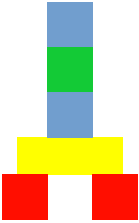
\includegraphics[scale=0.20]{figures/chapter2/task_goal.pdf}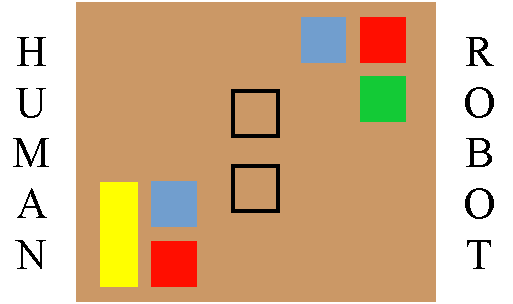
\includegraphics[scale=0.18]{figures/chapter2/task_setup_mini.pdf}}   
	\fancyhead[RO]{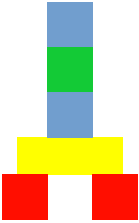
\includegraphics[scale=0.20]{figures/chapter2/task_goal.pdf}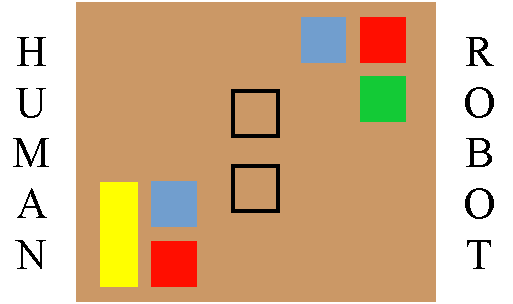
\includegraphics[scale=0.18]{figures/chapter2/task_setup_mini.pdf}\bfseries\thepage}  
	\fancyhead[RE]{\bfseries\nouppercase{\leftmark}}      % Chapter in the right on even pages
	\fancyhead[LO]{\bfseries\nouppercase{\rightmark}}     % Section in the left on odd pages
}%

\usepackage{pdfpages}
\usepackage{makecell}
\usepackage{pdflscape} 
\usepackage{mathtools}
\usepackage[section]{placeins}
\usepackage{afterpage}

%%%%%%%% my commands
\newcommand{\etal}{\textit{et al}.}
\newcommand{\ie}{\textit{i.e.}, }
\newcommand{\eg}{\textit{e.g.}, }
\newcommand{\fact}[3]{\mbox{\textit{#1}(#2, #3)}}
\newcommand{\circledtext}[1]{\raisebox{.5pt}{\textcircled{\raisebox{-.9pt} {#1}}}}
\newcommand{\sparql}{\textsc{SPARQL}}

\newcommand{\algConst}[1]{${\scriptscriptstyle #1}$}
\newcommand{\algNormTextSub}[2]{$\text{#1}_{#2}$}

\newcommand{\aslnumber}[1]{$#1$}
\newcommand{\aslstring}[1]{\textsf{#1}}
\newcommand{\aslvar}[1]{\textcolor{purple}{\textit{#1}}}
\newcommand{\asllabel}[1]{\textbf{#1}}
\newcommand{\annotation}[1]{{\footnotesize #1}}
\newcommand{\rulebody}[1]{\mbox{\hspace{.05\linewidth}}\begin{minipage}[t]{0.9\linewidth}#1.\end{minipage}}
\newcommand{\context}[1]{\begin{minipage}[t]{0.9\linewidth}#1\end{minipage}}
\newcommand{\planbody}[1]{\begin{minipage}[t]{0.9\linewidth}#1.\end{minipage}}
\newcommand{\Jason}[0]{\textbf{\textit{Jason}}}
\newcommand{\sn}{\mbox{\large\textbf{\texttt{\textasciitilde}}}}


\sloppy
\begin{document}
\setcounter{chapter}{2} %% Numéro du chapitre précédent ;)
\dominitoc
\faketableofcontents
\fi

\chapter{A direction-giving robot in a mall}
\label{chapter:chap3}
\minitoc

This chapter is from an article submitted to the  User Modeling and User-Adapted Interaction (UMUAI) Journal. This work has been achieved in collaboration with Guillaume Sarthou, Guilhem Buisan, Phani-Teja Singamaneni, Yoan Sallami, Kathleen Belhassein, and Jules Waldhart. In this chapter, we first give an overview of the European H2020 Project \acrfull{mummer}\footnote{\url{http://mummer-project.eu/}}. We then present the components developed by the LAAS-RIS team. My technical contributions are the Supervisor component, the component integration, the overall system debugging, the real-world deployment and the user study.

\section{Introduction}

In large scale indoor environments, like museums, shopping malls, or airports, the presence of large interactive screens, maps, or signs underline the importance of providing information on itineraries. However, orienting and reading maps to find one's own way may be challenging. As for signs, the wanted written information may not be within sight. People also look for information not available on visual media such as the location of a given product. That is where the robot has a role to play, bringing a new way to help people to get their bearings in large indoor environments such as shopping malls.

Therefore, in the context of the European H2020 Project \acrshort{mummer}\footnote{http://mummer-project.eu/}, we developed and deployed a social service robot in one of the largest malls of Finland, Ideapark in the city of Lemp\"a\"al\"a. This social robot is able to engage, chat with people, and guide them. We will not talk about the two first mentioned behaviors, developed by our project partners, but focus in this paper on the direction-giving.

As the mall has approximately 1.2 kilometers of shopping and pedestrian streets and more than 150 shops, people get easily lost. In such a large environment, having a robot guiding customers to their wanted destination would be time-consuming for the robot and would prevent this resource to be available for as many customers as possible. Inspired by the manner in which the mall employees perform this activity, we chose the solution to have a robot not accompanying people to their desired destination but rather verbally describing the route while grounding it with pointing gestures. If necessary, it moves a few meters inside its dedicated area (Figure~\ref{fig:chap3_pepper_mall}) to improve the perspective sharing with the human when pointing at a landmark, and therefore to improve the human understanding of the route. These features are unique to a robot and cannot be found on a map or an interactive screen. To endow the robot with such abilities, we built a complete implementation of a robotic architecture that has been deployed in a real-world environment, the Finnish mall. There, it ran for three months, three days a week.

All along the process, we elaborated and built the system based on the main principles and ingredients which have been identified and are investigated by the Human-Human Joint Action community. We also conducted preliminary studies and used the Joint Action perspective to analyze how human guides would achieve such an activity at the place where the robot was intended to be deployed. This was possible essentially because we were able to combine the results of the JointAction4HRI\todo{to remove once written in chapter 1}\footnote{It is a multi-disciplinary project which gathers philosophers, developmental psychologists and roboticists. \url{https://jointaction4hri.laas.fr/}} project with the \acrshort{mummer} project.

Our claim is that such an approach is relevant in the way the joint action principles provide pertinent guidelines and it is possible to effectively elaborate models and implement systems based on them. 
The output is a complete robot architecture that integrates a number of components implementing the main decisions and behaviors which have been identified. Each of them makes use of various models and decisional algorithms, all integrating explicitly human models and joint action principles and mechanisms.


The chapter is constructed as follows. In Section~\ref{sec:related-work} we provide background information about robot guides and direction-giving task and discuss about how the human partner has been considered. In Section~\ref{sec:rationale} we discuss how we model the direction-giving task as a human-robot joint action. We analyse the task based on human-human exploratory studies and decompose it into a succession of precise subtasks in Section\ref{sec:modeling}. An overview of the resulting architecture and a description of its components are presented in Section~\ref{sec:globalarchi}. Then, we present in Section~\ref{subsec:archi-integration}, the integration of the overall architecture into a physical robot and the steps until its final deployment ``into the wild''. In Section~\ref{sec:qoi_integration}, we show how we used this task to implement the QoI Evaluator presented in Chapter~\ref{chapter:chap2}. Finally, we present the user study we performed with 35 participants and its results.

\begin{enumerate}
	\item March 2018: beginning of the design and implementation of the direction-giving task
	\item September 2018: First tests of the task on the field, \ie in a Finnish mall
	\item June 2019 and September 2019: New tests of the direction-giving task on the field
	\item From September to December 2019 (project formal end): The robot autonomously ran three days a week in the mall (with only remote monitoring of the robot performance by our team for debugging and tuning)
	\begin{enumerate}
		\item November 2019: Integration in the \textit{Supervisor} of a preliminary version of Quality of Interaction Evaluator implementing the model described in Chapter~\ref{chapter:chap2} \\ $\Longrightarrow$ version 1 of the QoI Evaluator
		\item From November 2019 to December 2019: Around 350 direction-giving tasks were performed with usual mall customers. Bug corrections and tuning of the direction-giving task. This allowed us to improve the QoI Evaluator thanks to: \begin{enumerate*}[label=(\roman*)] \item data collection of task failures and standard durations of the subtasks executions \item lessons drawn about metric definitions and choices. \end{enumerate*} \\ $\Longrightarrow$ version 2 of the QoI Evaluator\label{list:mall}
	\end{enumerate}
	\item January 2020: User study with 35 participants to compare three direction-giving task robot behaviors, allowing to log interactions at the same time we could monitor them\footnote{The QoI Evaluator was running in background, it was not the purpose of the study.}. End of the project.\label{list:tests}
	\item March 2020: Refinement of the QoI Evaluator, \ie improvement of the metric functions and tuning of their parameters. In the lab, with the same direction-giving task than the one used in the mall, comparison of the QoI computed by the robot when it is dealing with an ``ideal'' human, a ``confused'' human and a ``non-compliant'' human. \\ $\Longrightarrow$ version 3 of the QoI Evaluator\label{list:refin}
\end{enumerate}

\section{Related work}
\label{sec:related-work}

A number of contributions have proposed robot guides, from the first museum guides \cite{burgard_1999_museum, thrun_99, siegwart_2003_robox, clodic_2006_rackham} to more recent robot guides in large areas \cite{bauer_2009_autonomous, triebel_2016_spencer}. For example, \cite{chen_2017_robots} presented a guiding robot in a shopping mall where it accompanied the customer to the desired location and pointed at the shop. Another example is a shopping robot helping people to find products among the aisles of a store \cite{gross_2009_toomas}. 
However, the focus in these contributions is mainly the fact that the robot is challenged to navigate until the goal destination with the presence of humans. Efficient mapping and localisation in large areas, social navigation are the main concerns. This is different from our needs where the robot is voluntarily constrained for its motion to a limited area with a focus on conveying to the human the pertinent information to reach by herself the desired place.

Direction-giving tasks have been investigated in the human-robot interaction community. \cite{kopp_2007} describes an embodied conversational agent giving route directions using deictic gestures. A number of key contributions have been developed over the years by ATR-IRC within the Robovie robot and project.  First, \cite{okuno_2009_providing} developed a model for a robot providing route directions, integrating utterances, gestures, and timing. The experiments explored the influence of gestures and highlighted the importance of timing in the directions-giving task. Then, \cite{kanda_2009_affective, kanda_2010_communication} implemented a guiding behavior as part of a wider system with the robot pointing toward the first direction to take and saying ``please go that way'' and then, continuing its explanation by saying ``After that, you will see the shop on your right.''. Their robot also gave recommendations for restaurants and shops based on customer tastes. In their following work, \cite{morales_2011} presented a route perspective model attempting to represent humans' concept of route and visibility of landmarks, which they believed to match people's perception of the environment. Then, \cite{matsumoto_2012_you} developed a robot able to follow a user while inferring their memory recall of shops in the visited route. When the user asked the location of other shops, it gave the route description with references to the known locations inferred with the model of the user's memory recall. Finally, \cite{satake_2015_should} showed a complete architecture of an information-providing robot able to move around a square in a mall composed of: a map, an ontology, a speech recognition system (operated), a dialog manager, a localization module, and a people tracker. As in their previous works, the robot verbalized utterances and used deictic gestures to give route directions. 

Let us also mention \cite{bohus_directions_2014}, a robot providing verbal directions to people using deictic gestures coupled with spoken references. For example, the robot said ``Go to the end of this hallway'', executing a pointing gesture at the same time, and then continued the explanation with sentences such as ``Turn right and keep walking down the hallway''. \cite{iocchi_2015_personalized} mentioned both guiding and direction providing as use cases of their system.

Numerous other contributions can be found but,  only a few of them propose full architectures for an autonomous direction-providing robot, the most complete one being the Robovie robot presented above. 

Still, to the best of our knowledge, no system tackles the overall guiding-task with flexibility. Indeed we claim that it is important for the robot
to reason about the current and desired perspectives of the human and the robot and to be able to pro-actively propose to the human a pertinent placement. This is one of the basic bricks of our system and it is strongly linked to the key principles of Joint Action which involve the ability to establish and monitor joint attention,  and to conduct a multi-step task achievement involving contributions of both agents. Besides, it is the duty of the robot to permanently adapt to human needs and preferences and to synthesize acceptable behaviours.

\section{Rationale}\label{sec:rationale}

We briefly summarize here the main issues involved in Joint Action which we exposed with more details in \ref{chapter:chap1}. 

The design of our system has taken into account the results of several user studies involving human guides of the mall (see Section~\ref{sec:modeling}). Indeed, it could be of interest to have a robot performing in the same way as a human guide does.  ``If robots could display predictable behaviours that are in line with human's expectations based on their models of human joint action, the resulting interaction would achieve greater naturalness''~\cite{curioni_2017_joint} and ``human agents would then be able to apply predictive and adaptive processes acquired in human interactions to the interaction with robots''~\cite{curioni_2017_joint}. Here, we also take advantage of the fact that the robot is a humanoid and the human anthropomorphizes the robot behaviour (whatever we do).
However, it is not always possible or desirable for a robot to imitate what a human would do at its place. It could let people think that the robot has more capabilities than it really has. In that way, besides the imitation, it could be desirable for the robot to exhibit its limitations, e.g. saying that it is able to provide you direction into the mall (and nothing else).

Participating agents in a joint action need to represent not only what they will do but also what will be performed by the others. Doing so, they also need to be able to consider the combined effects of their respective actions~\cite{pacherie_2012_agency}. Joint action involves representations of the other agents who are actually and potentially involved. Shared task representations provide control structures that allow agents to flexibly engage in joint action~\cite{knoblich_2011_joint}.

In our task, the robot has a role, it is a guide and the human is a customer with a need to find a direction. The joint action is not symmetric, there is a difference of knowledge and skills between the two agents. \cite{curioni_2017_joint} raises the fact that ``task asymmetry is an important factor to consider when investigating complex joint action settings because it drives the systemic emergence of communication and coordination dynamics (for example in the form of task distribution)''. At the supervision level (see Section~\ref{subsec:supervision}), we modelled which part of the task falls to the robot and which part of the task falls to the human. We could also infer that knowing the robot role as guide, the human would be able to infer what it is entitled to do. This way, we could consider that they share the route description task representation. 
Another important point is that ``shared task representations not only specify in advance the individual parts each agent is going to perform but they also govern monitoring and prediction processes that enable interpersonal coordination in real time.''~\cite{knoblich_2011_joint}. Our system handles that monitoring and prediction in its supervision component(see Section~\ref{subsec:supervision}).


Joint attention provides a mechanism to form shared perceptual representations of the situation. ``The phenomenon of joint attention involves more than just two people attending to the same object or event. At least two additional conditions must be obtained. First, there must be some causal connection between the two subjects’ acts of attending (causal coordination). Second, each subject must be aware, in some sense, of the object as an object that is present to both; in other words, the fact that both are attending to the same object or event should be open or mutually manifest (mutual manifestness)''~\cite[p.~355]{pacherie_2012_agency}.

As explained above, joint attention comes with two requirements: causal coordination and mutual manifestness. We can consider that the engagement in the interaction session represents the causal coordination. Then, at least on the robot side, we could argue for mutual manifestness. Indeed, as we will explain, we give the robot perspective-taking abilities, and abilities to find out where and how the human and itself should be placed to share a joint attention relative to a landmark. With those requirements fulfilled, ``by attending jointly, co-actors establish perceptual common-ground and become aware of each other's action opportunities and constraints''~\cite{curioni_2017_joint} (they also use the expression ``spatio-temporal common ground''). Joint attention and in fact in our case, the overall interaction process by itself (aka its unfolding), could be seen as an continuous process sustaining under-construction common-ground.

In our system, the situation assessment component provides visuospatial perspective-taking. It computes, from the robot point of view, a number of facts regarding what the robot is looking at, which landmark is visible to it, what is present at its proximity, etc. It also computes the same information from the perspective of the person interacting with it. This way the robot is able to infer, based on its own models, which information is shared (or not) with the person it interacts with.


\section{Designing direction-giving behavior in a shopping mall}
\label{sec:modeling}

\begin{figure}[!t]
	\centering
	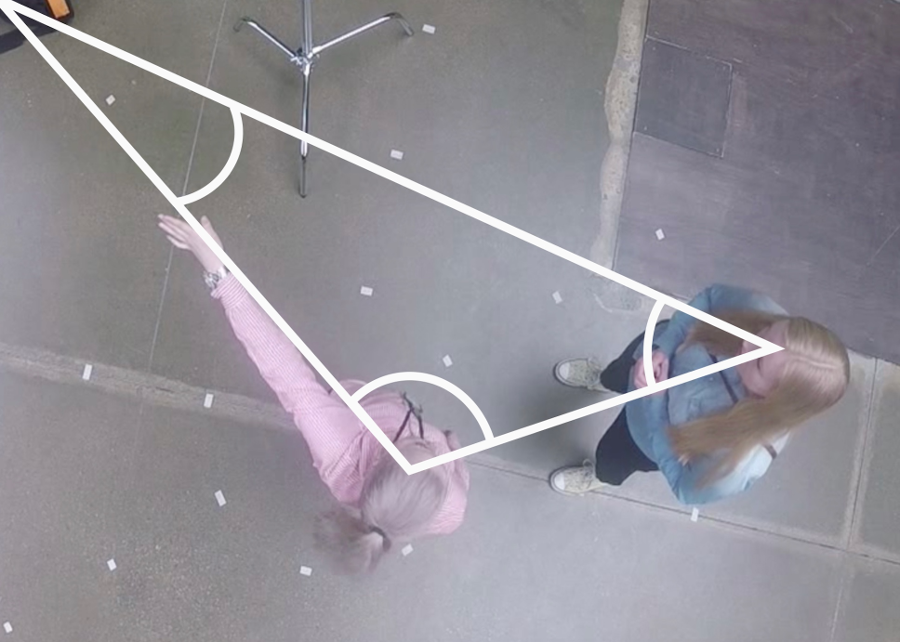
\includegraphics[scale=0.7]{figures/chapter3/human_guide.png}
	\caption{\label{fig:chap3_human_guide} Picture from the second Human-Human study \cite{belhassein_2017_human}. Here, the guide is giving the route description to reach a given shop by pointing at it. Positions regarding the target and the customer, as well as gazes and pointing gestures, were analyzed.}
\end{figure}

\subsection{What we learnt from humans}\label{sec:methodology}
In order to inform the design and implementation of the pertinent functions and their articulation, two human-human exploratory studies were conducted in collaboration with VTT Technical Research Centre of Finland. It allowed us, in addition to the study of the existing literature, to enrich our knowledge on effective route descriptions and how they can be used in the very context of the actual robot deployment environment. 

The first pilot study consisted in a human guide providing route information. It was carried out close to the future location of the robot in order to avoid biases linked to the location or the environment. Based on preliminary interviews with guides working at Ideapark, a list of 15 shops often requested by customers was selected. The preliminary experiment consisted of one participant asking for shop directions to a guide working at the mall information booth. Two researchers, as participants, and two guides took part in the experiment. The two guides were instructed to give guidance as they would normally do. The situations were video recorded and the guides were briefly interviewed after the sessions. The video analysis focused on non-verbal communication, and in particular the different types of gestures used to give guidance, the positions of the two protagonists in relation to the target shop and their interlocutor, and the gazes alternation. \cite{belhassein_2017_human} gave the first indications to consider for the robot guidance to be effective and understood by customers, resulting from this pilot study. For example, this pilot study allowed us to notice a preferential use of the ipsilateral hand to the visual field of the target. In line with the existing literature on gestures studies, we also noticed that deictic gestures were naturally more frequent than iconic gestures or beats, while metaphorical gestures were rare. As shown by~\cite{allen_2003}, the hand used to point a referent was oriented vertically in the case of stores (vertical referents) or directed actions such as a path to take or turns, whereas in the case of horizontal referents (e.g. escalators), the hand was oriented horizontally (palm facing the ground).

A second exploratory study was then carried out adding complex situations (e.g. two customers requesting directions at the same time, two different shops in the same request, or someone who interrupts the conversation between the guide and the customer). Again, social signals were analyzed (see Figure~\ref{fig:chap3_human_guide} for an example). The protocol used and the results have been published~\cite{heikkilae_2018_where,heikkilae_2019_should}. By analyzing the sequencing of the whole interaction, this second study showed the guide pointing the general location of the target first, before explaining and pointing the different stages of the path to take to get there. Then, the sequencing of the route description itself showed that a first deictic gesture on a visible passage (corridor, or if the shop requested is on the second floor, the escalator) preceded the explanations about the directions to take. The most interesting results concerned situations of confusion and misunderstandings. Indeed, several elements might be sources of confusion for the customer, such as using only one transmission channel (e.g. gesture without speech), the choice of landmarks which are not always appropriate, if there are several route descriptions in the same explanation, or when the distance is not specified. 

\subsection{Design of the collaborative task for a direction-giving robot}\label{sec:guiding}

From the analysis of human-human direction-giving and through an iterative design process, we designed and implemented our directions providing robot. Our model of the collaborative task can be represented as a succession of subtasks, as shown in Figure~\ref{fig:chap3_HTN}. This figure also exhibits the incremental refinement of the task into a sequence of human-robot interactive actions. The aforementioned subtasks are:

\begin{figure}[!t]
	\centering
	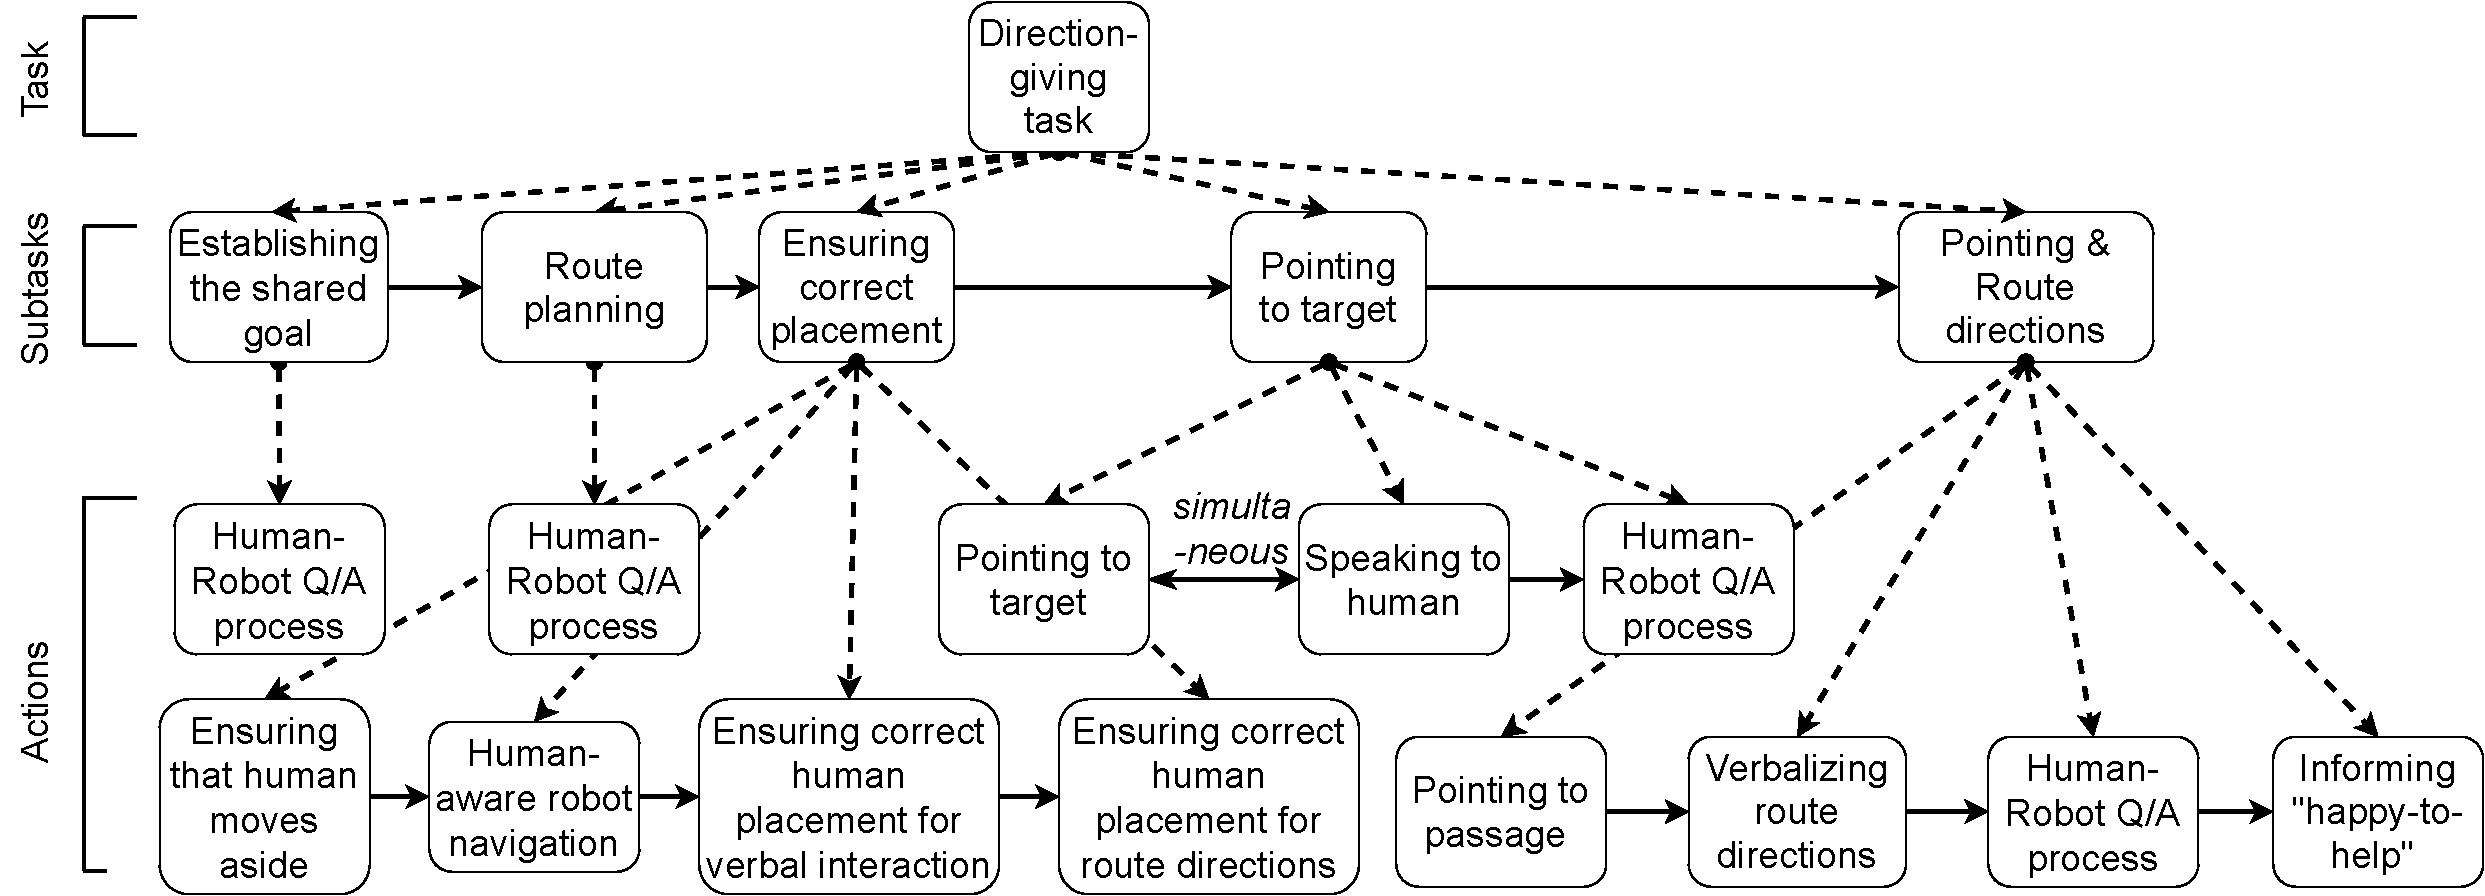
\includegraphics[width=\linewidth]{figures/chapter3/HTN-guiding_task.pdf}
	\caption{The representation of the direction-giving task as a hierarchical task network with task, substasks and actions levels. All the horizontal arrows are sequential links and the rest are decomposition ones.}
	\label{fig:chap3_HTN}
\end{figure}


\begin{enumerate}
	\item \textbf{Establishing the shared goal}: In this first step, the human and the robot negotiate and establish a shared goal. Specifically, the robot tries to determine precisely the place -- we called it the \textit{target} -- it should give directions for. This is immediately completed if the human directly asked for a known shop. Several verbal exchanges can be necessary in case the person asked for a kind of shop (e.g. restaurant) or a product or in case the robot has not properly understood the name of the place and needs to disambiguate.
	\item \textbf{Route planning according to the human willingness and ability to climb stairs}: As the robot role is to help people, adapting to them, it needs to ensure that they have the abilities to follow the route it will indicate to them. So, first the robot computes the best route to the target and then checks the presence of stairs in it. In case there are, the robot enquires whether the human can or want to climb them or not. If they cannot or do not want to, the robot computes a new route without any stairs. The planned route contains a first  \textit{passage} (\ie a corridor, a door or an escalator) which the robot will try to point.
	\item \textbf{Ensuring correct placement}: The second human-human study, mentioned in Section~\ref{sec:methodology}, highlighted the fact that human guides point to a visible \textit{passage} before giving the route directions. Thus, we endowed the robot with this ability as described further in the item~\ref{steps:passage} of this list. In order to be in good conditions while performing this item \ref{steps:passage}, that is to say to ease the human understanding of the directions, the robot seeks better positions for the human and itself. It does so by computing a position for the human, considering their visual perspective of the passage.
	%Clearly, it does not planned a new position if, from it, the human visibility of the passage is not higher than their current one.
	The robot computes a new position for itself as well, to form a triangle whose vertices are the planned robot position, the planned human position and the passage, as shown in Figure~\ref{fig:chap3_human_guide} and Figure~\ref{fig:chap3_dir_giving_task}. After having computed these positions, the robot moves, and as they both are engaged in the task, expects the human to join it once its position is reached; it calls them if they do not. As the human might not be at the exact position computed for them, the robot checks their visibility of the passage. In case their visibility is too low, the robot will adjust their position thanks to verbal instructions (\ie come closer, move back). Figure~\ref{fig:chap3_dir_giving_task} illustrates the initial and final positions of both agents, in a lab context. 
	\item \textbf{Pointing to target}: Following the sequencing obtained from the aforementioned human-human study, the robot first points in the target direction, along with a brief sentence. As the robot is a helper and it is involved in a joint action with the human, it needs to ensure that its actions produce their expected results. In this case, if the robot computed that the target should be visible from their position, it checks that the human has seen it, either by monitoring their perspective or by asking. In case of a negative answer, it will point again.\label{steps:ensuring}
	\item \textbf{Pointing to passage and giving route directions}: Still following the sequencing from the study, when the target is not in the same physical space as them, meaning that there is a passage on the way to the target, the robot points to this passage and then verbalizes the route directions. These directions take into account the orientation the human will have and describe the route (e.g., take the corridor on the left side). Finally, the way they are built (\ie the order of the steps, the keywords to use...) is also based on the human-human study. Here again, the robot ensures that the route directions have been understood by asking the person about it or if the passage has been seen if there is one.
	% 	(only one of the two questions is asked as with both one after the other, people interacting with the robot were annoyed). 
	In case of a negative answer, it will point and give the route directions again. Finally, the robot ends the task with a ``happy-to-help'' short sentence.\label{steps:passage}
\end{enumerate}


\begin{figure}[!ht]
	\centering
	\subfloat[Initial positions of the human and the robot. The human asked the robot for route directions to a target behind him.]{ 
		\begin{minipage}{\linewidth}\hspace{0.05\linewidth}
			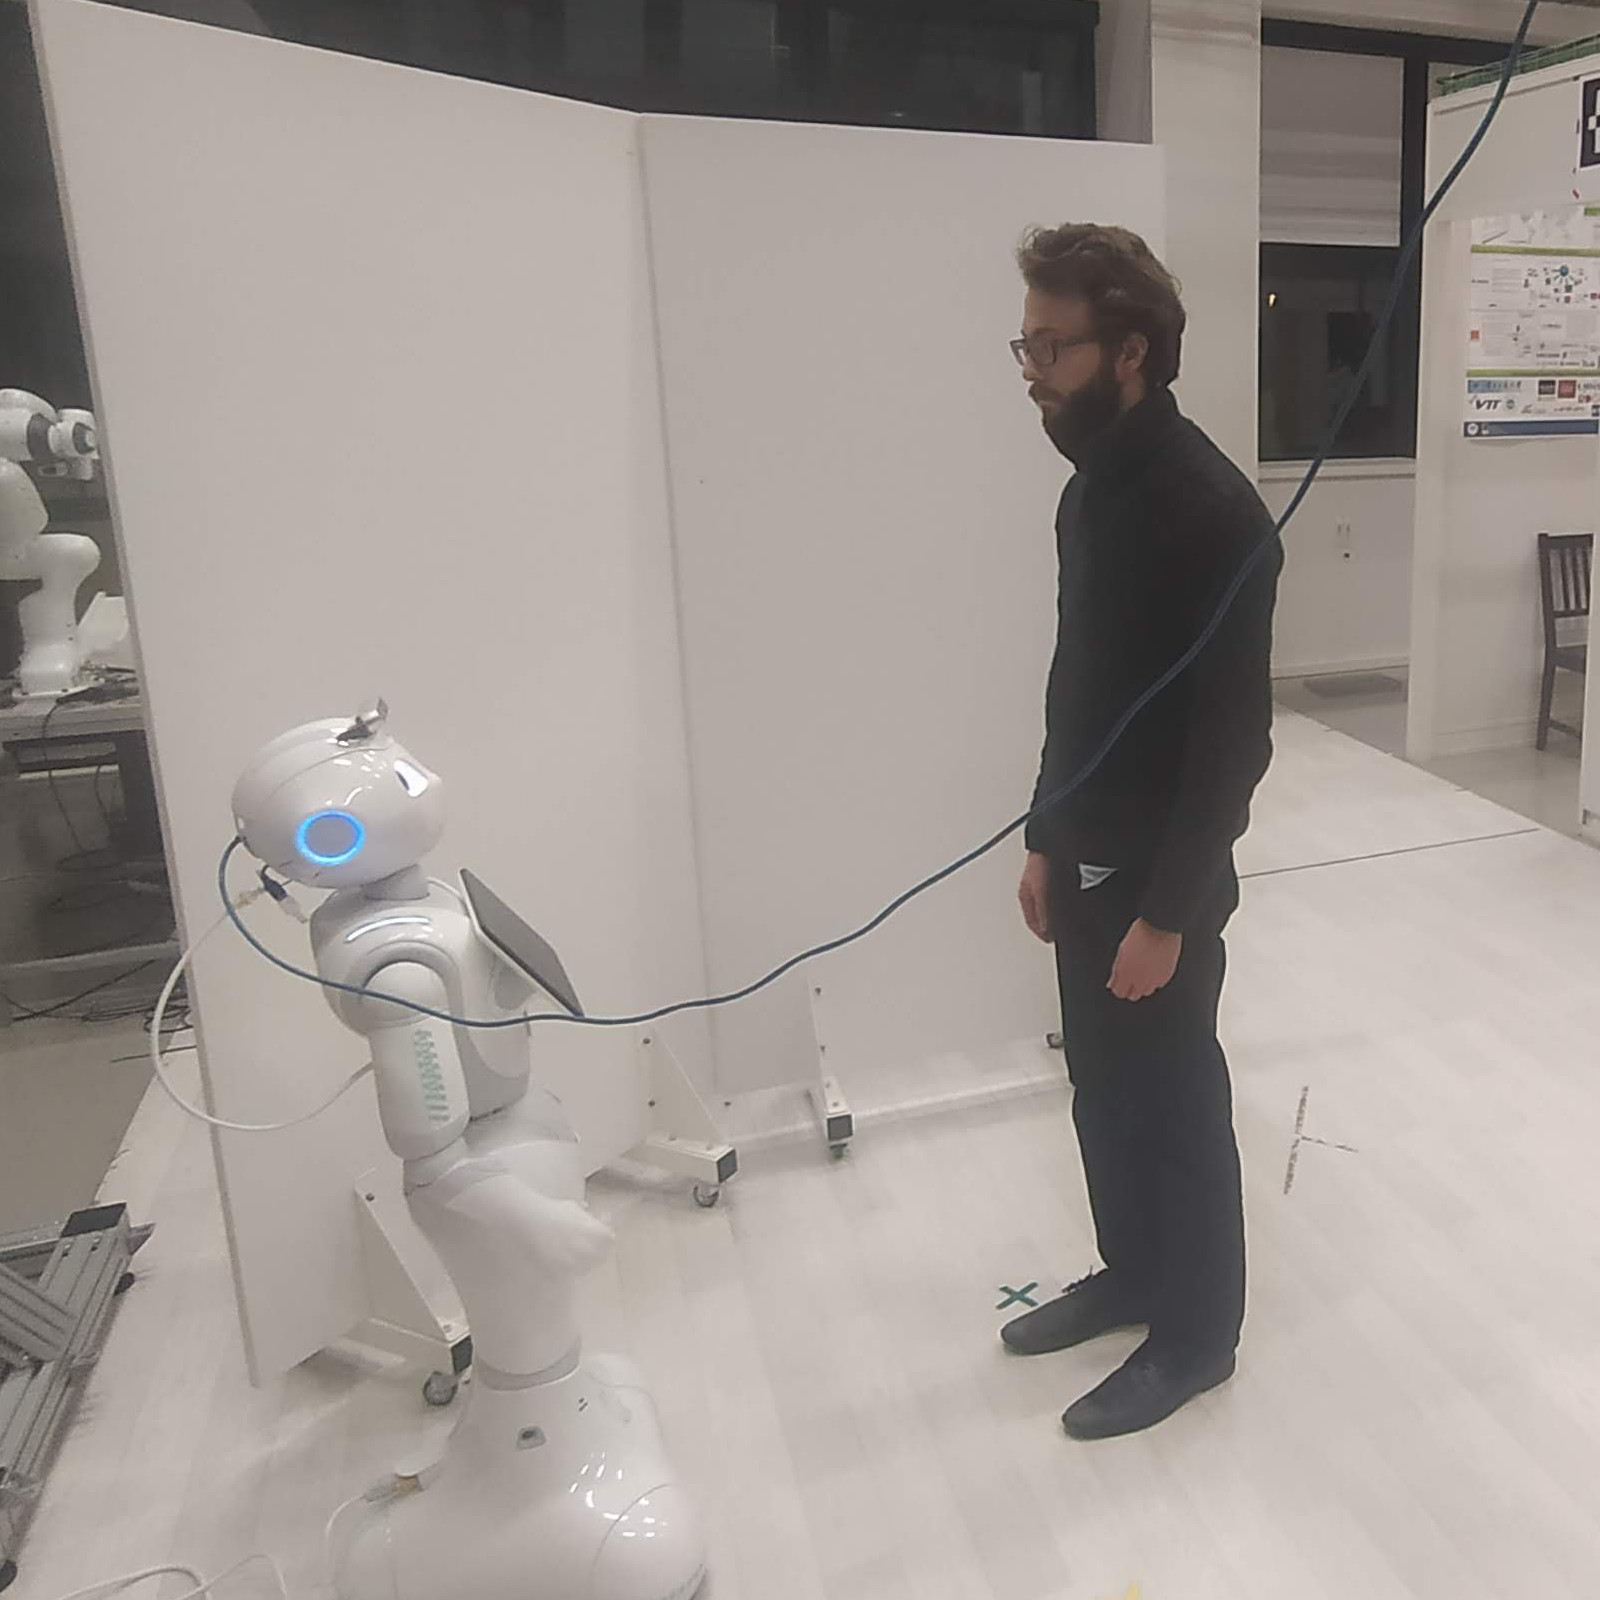
\includegraphics[width=.4\linewidth]{figures/chapter3/init_pose_r.jpg}\hspace{0.1\linewidth}
			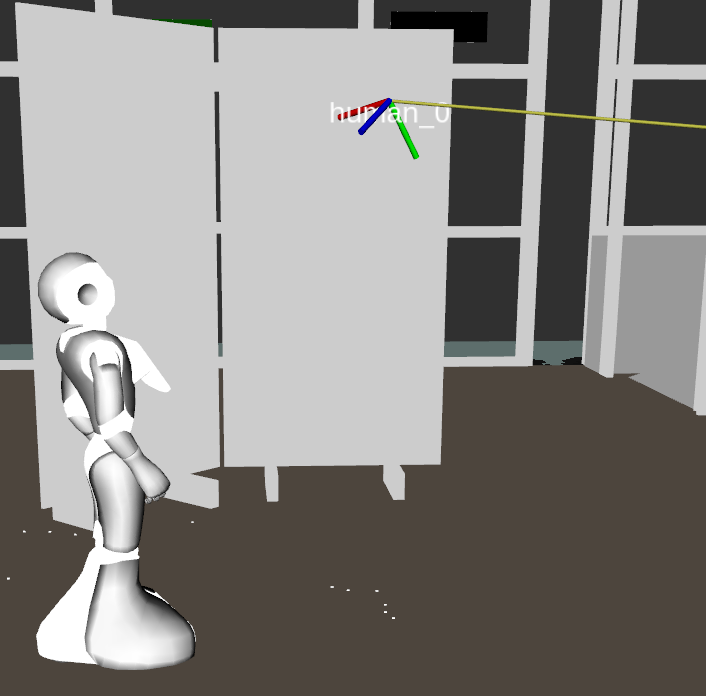
\includegraphics[width=.4\linewidth]{figures/chapter3/init_pose.png}
		\end{minipage}
	}\par\vspace{2ex}
	\subfloat[The robot and the human are in their final positions. The blue spheres are the computed position for the human by the robot. The robot is pointing to the passage (in blue frame). We can observe the triangle formed between the human, the robot and the passage (the blue area on the floor) as in Figure~\ref{fig:chap3_human_guide} where two humans are in a triangle formation.]{
		\begin{minipage}{\linewidth}\hspace{0.05\linewidth}
			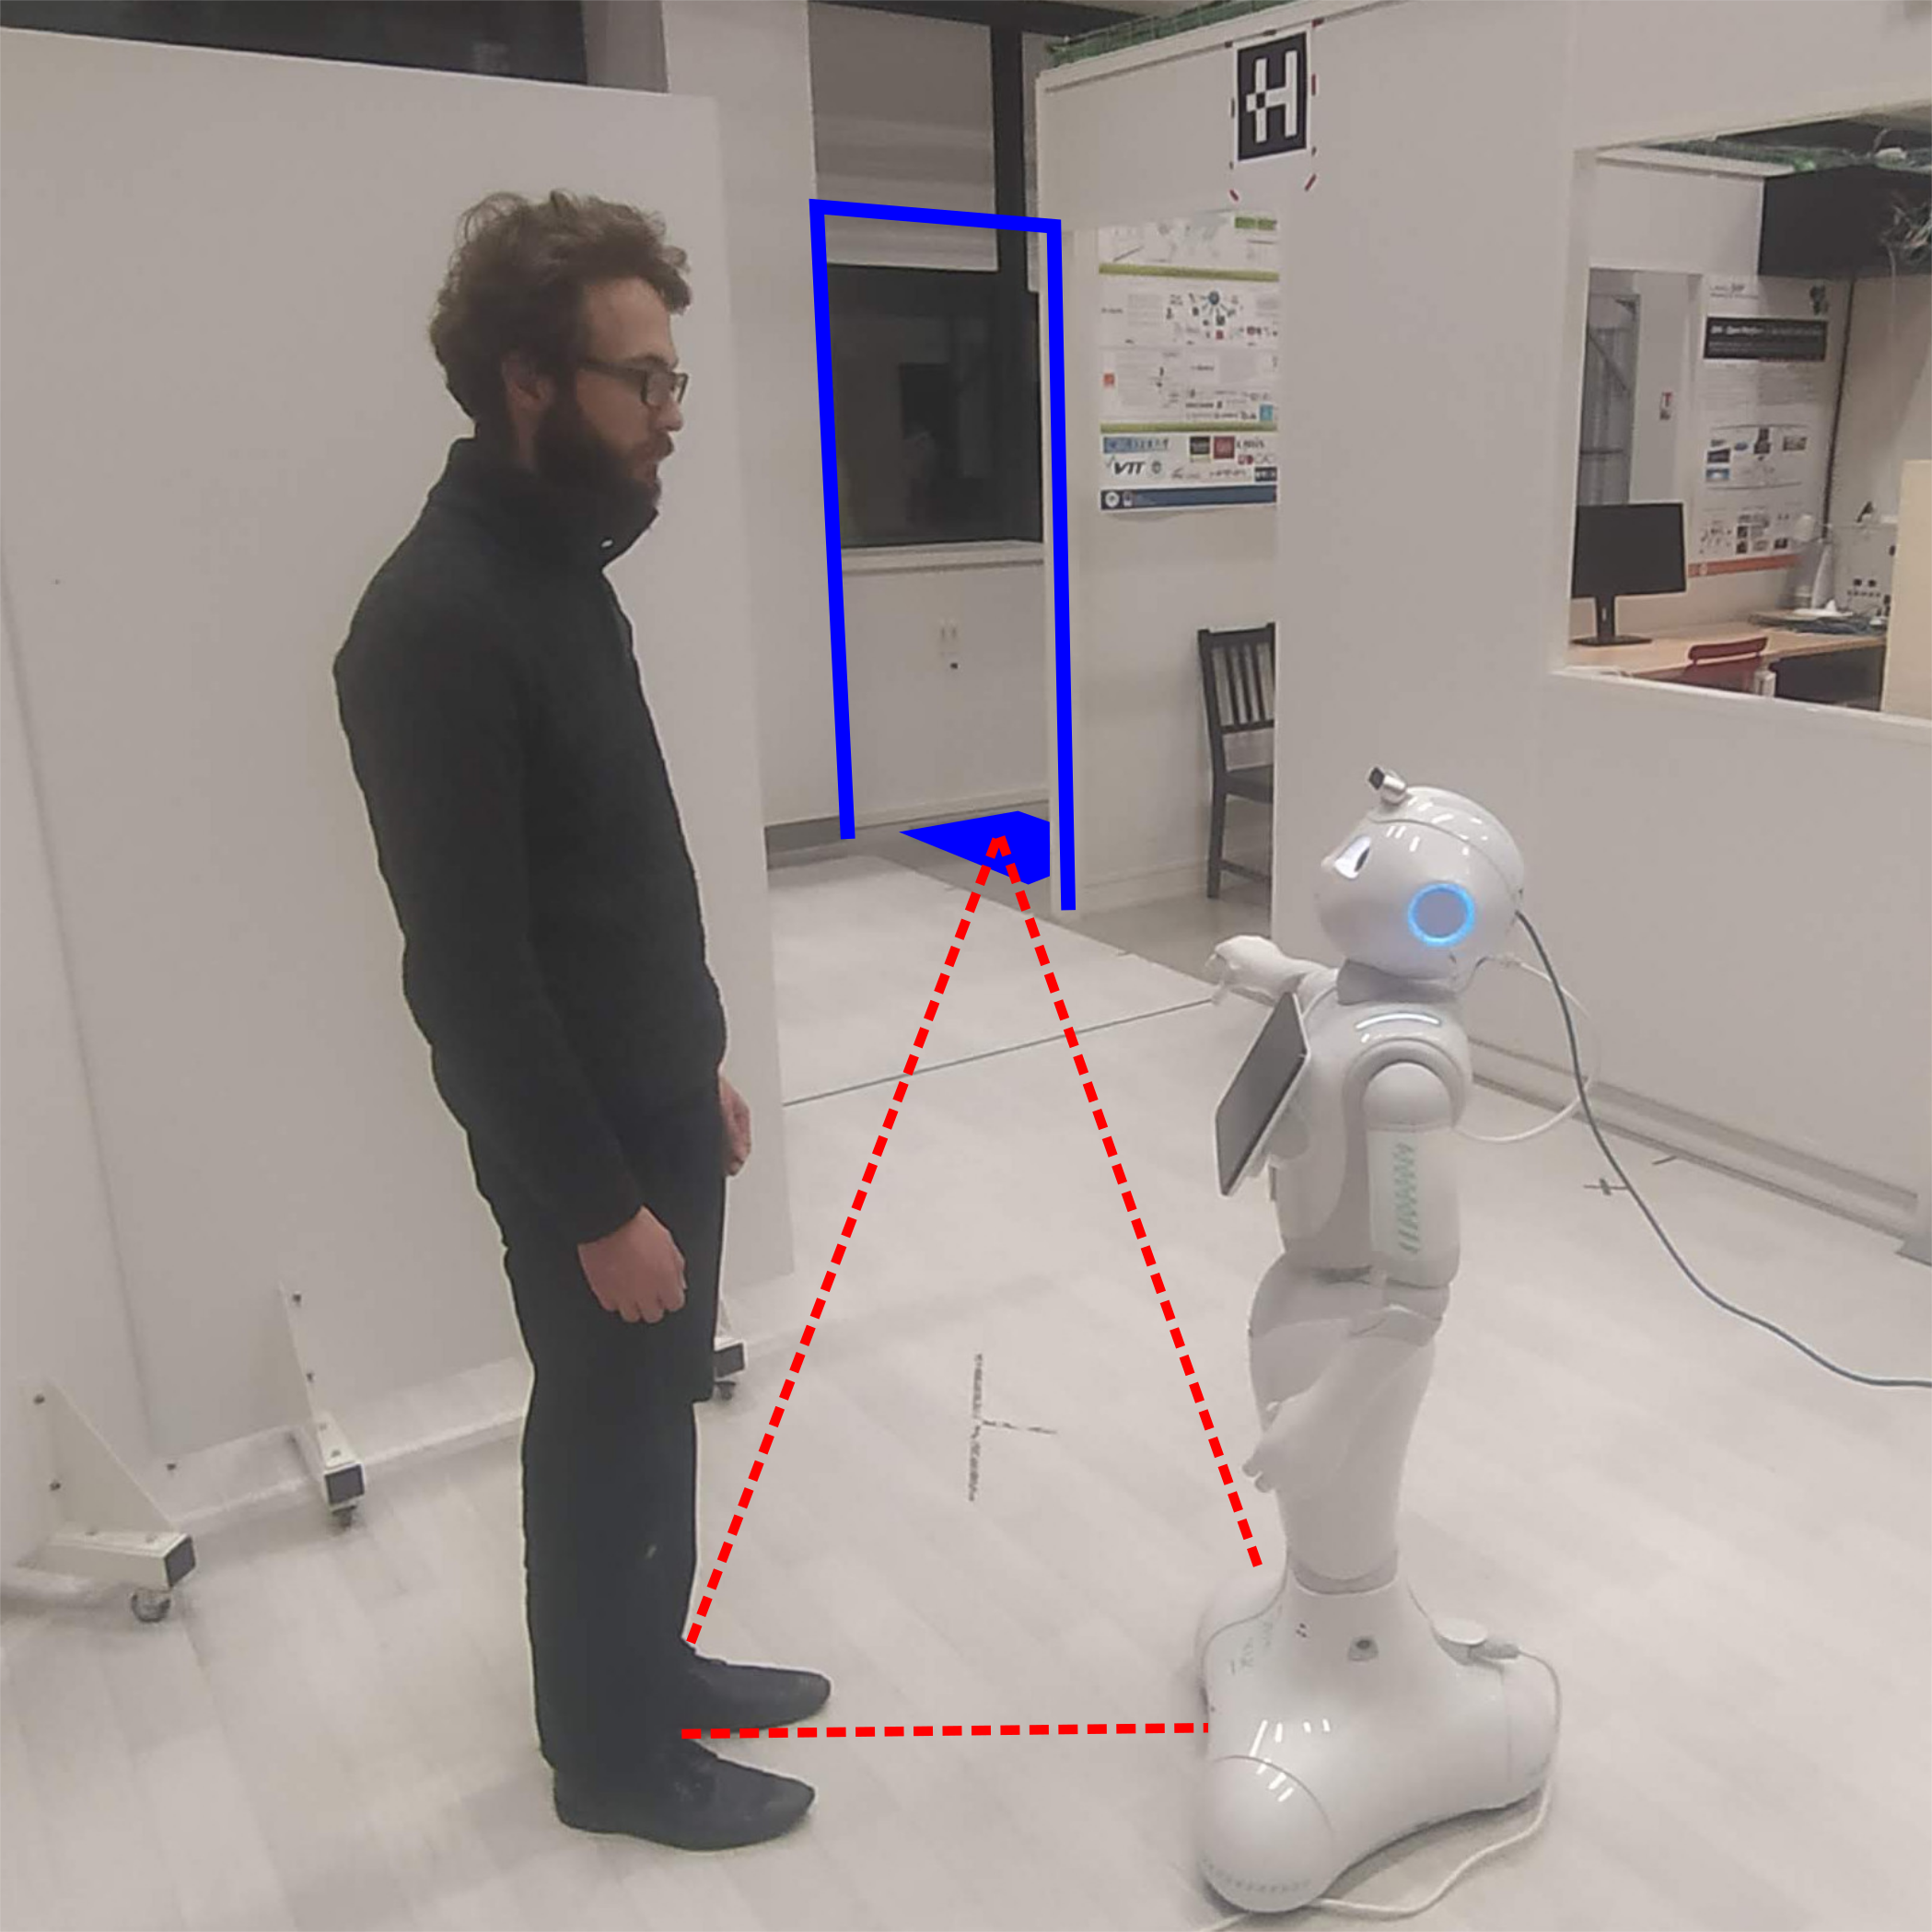
\includegraphics[width=.4\linewidth]{figures/chapter3/final_pose_r.jpg}\hspace{0.1\linewidth}
			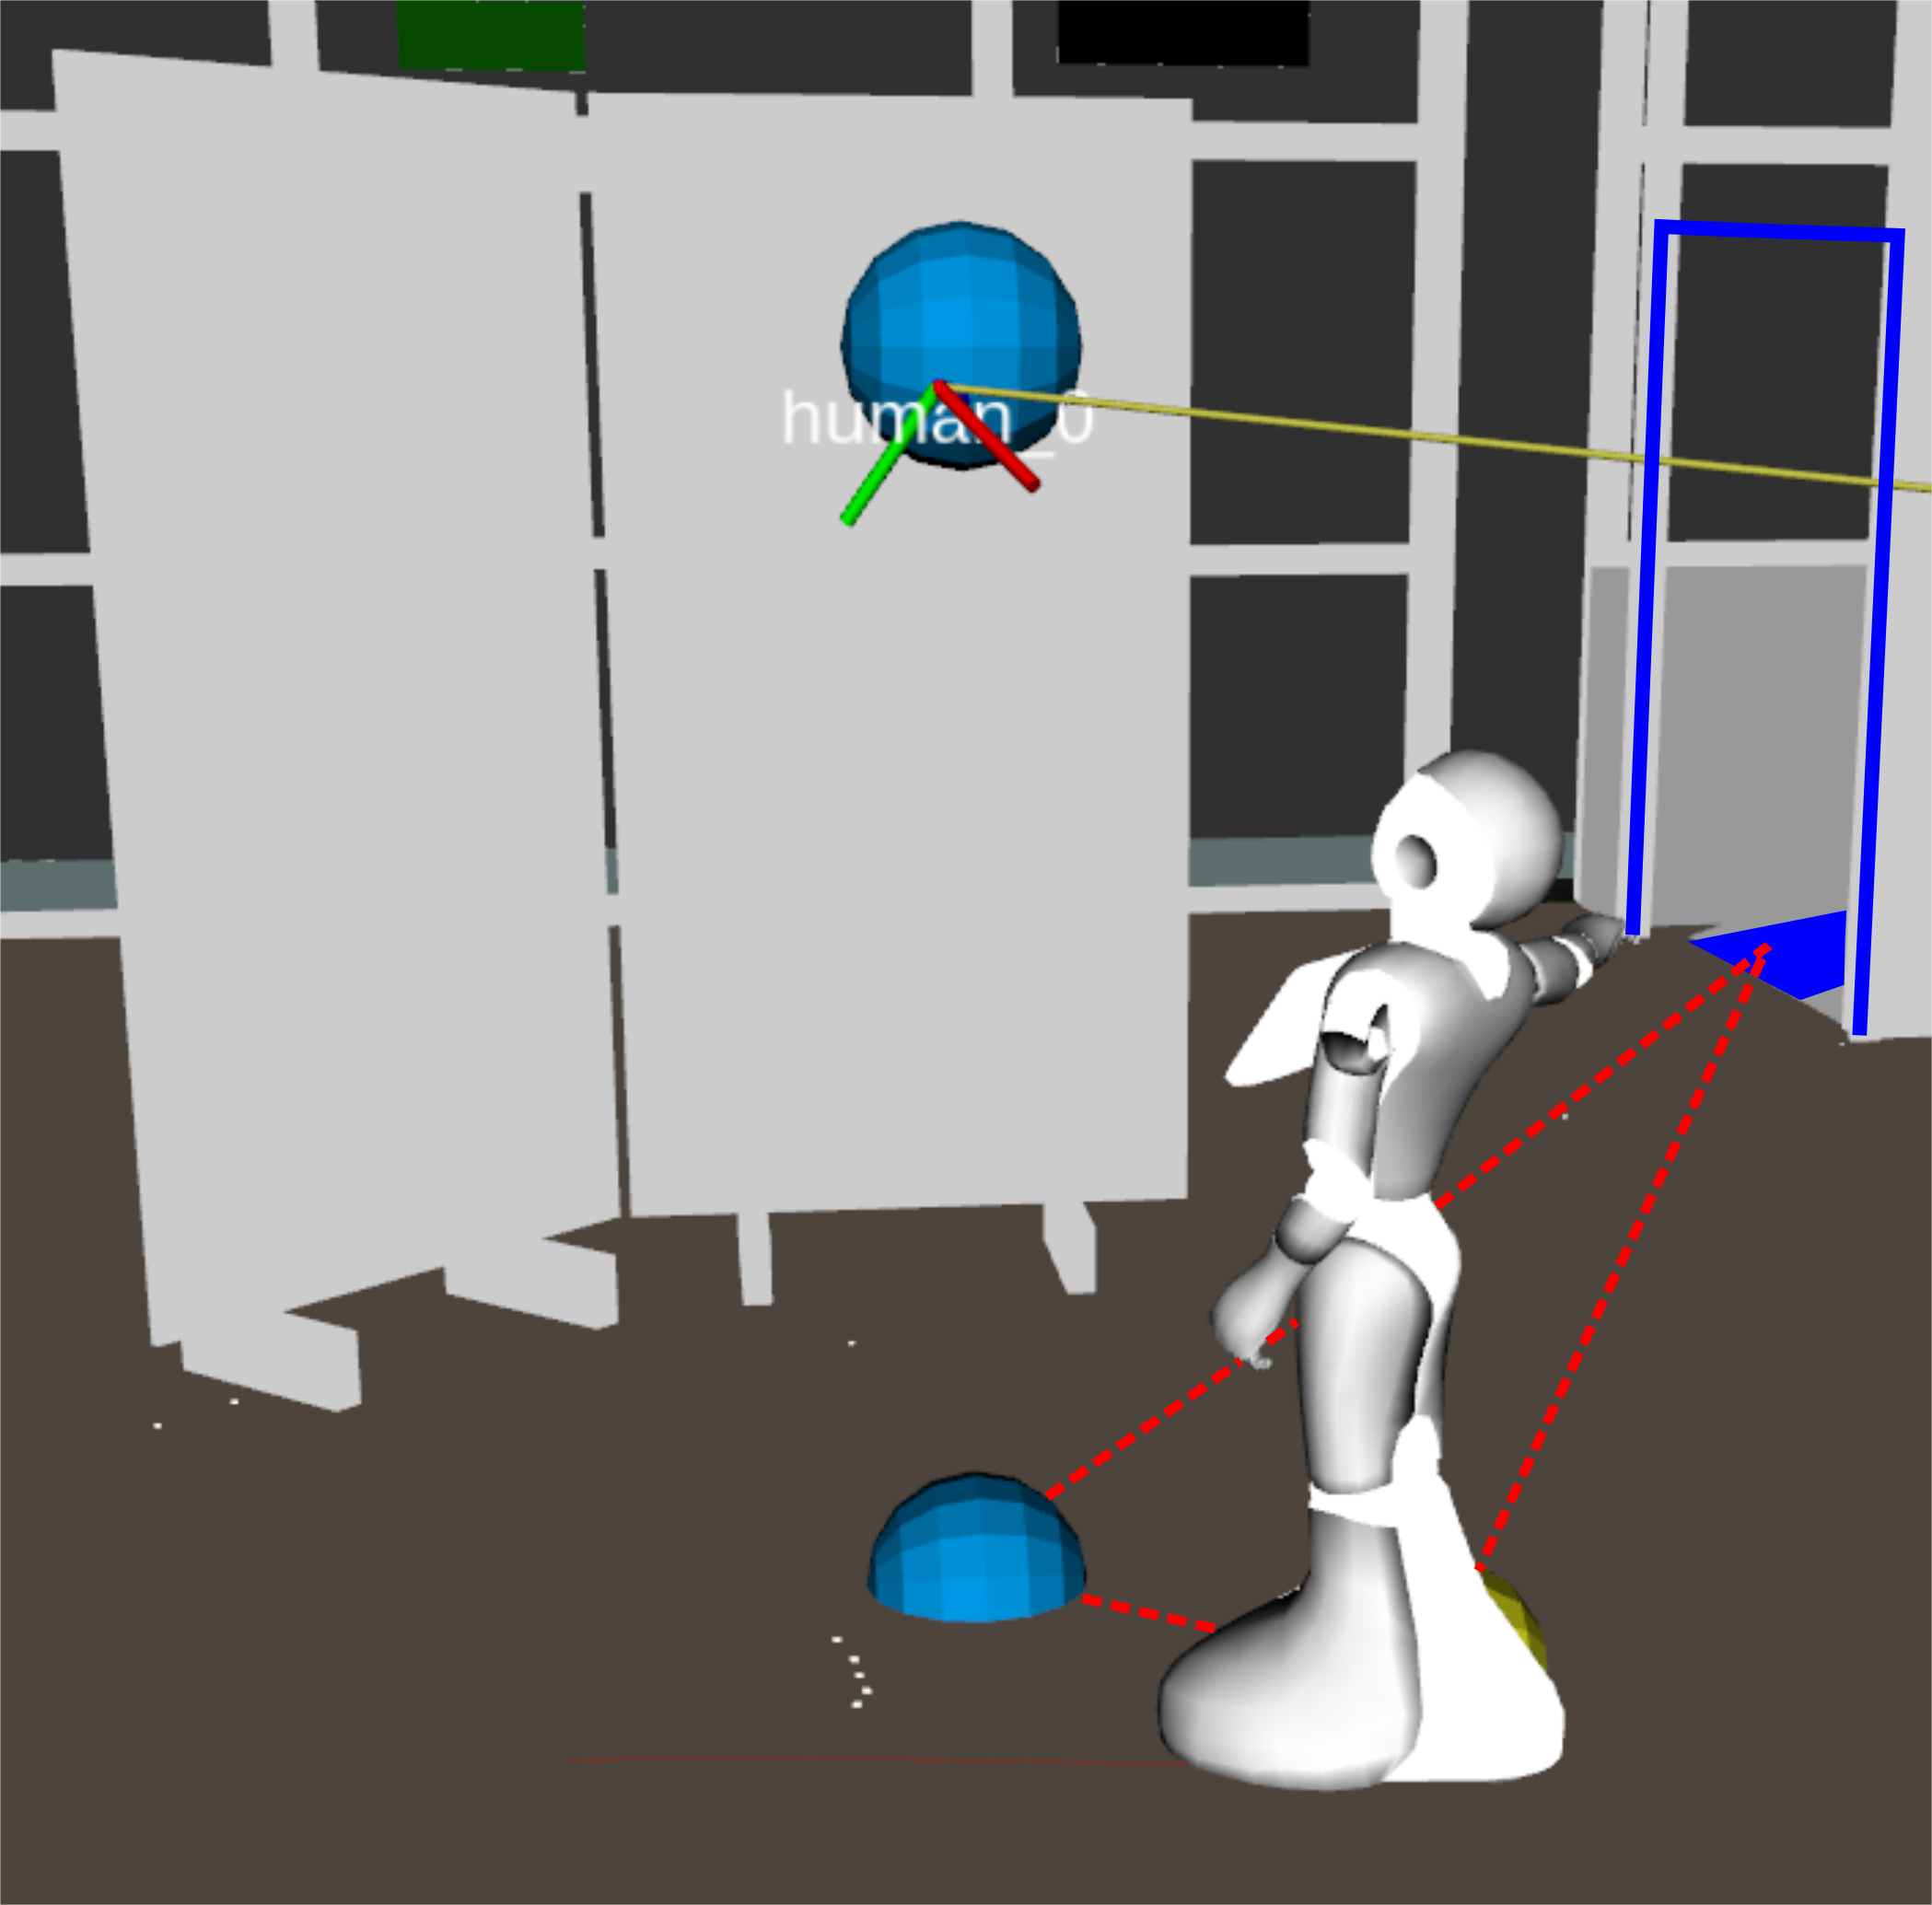
\includegraphics[width=.4\linewidth]{figures/chapter3/final_pose.jpg}
		\end{minipage}
	}\par  
	\caption[pos]{Initial and final positions of a direction-giving task in the lab context. On the left are pictures and on the right screenshots of Rviz\footnotemark (a 3D visualization tool for ROS.)}
	\label{fig:chap3_dir_giving_task}
\end{figure}


To endow a robot with the abilities described above, to build a robotic architecture embedding all these aspects, is a challenge. We tackled it with the architecture presented in the next section.

\section{The deliberative architecture}\label{sec:globalarchi}

In this section, we present the robotic architecture developed to handle the direction-giving task. This architecture relates to Beliefs, Desires, Intentions (BDI) architectures. As explain by~\cite{wooldridge_1999_intelligent}, such a kind of architecture is primarily focused on practical reasoning, meaning the process of deciding step by step which action to perform to reach a goal. 

\begin{figure}[ht!]
	\centering
	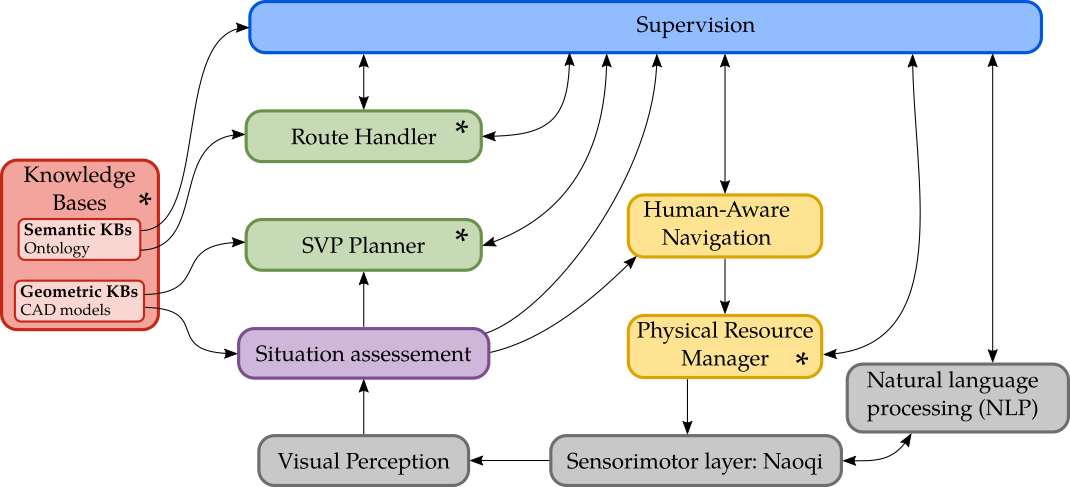
\includegraphics[width=\textwidth]{figures/chapter3/architecture.png}
	\caption{\label{fig:chap3_architecture} The general architecture developed for the robot guide. The components presented in this chapter are the colored blocks. The red components with the symbol * are the ones on which I participate. The visual perception and dialogue components have been respectively developed by IDIAP and HWU and are described by~\cite{foster_2019_mummer}. Naoqi is a Softbank Robotics software. }
\end{figure}

The figure~\ref{fig:chap3_architecture} represents the architecture, its components, and their interconnections. Communication between components relies on ROS. In this chapter, we only present the components developed by the LAAS-RIS team, represented by the colored blocks on the architecture. First, we present the two knowledge representations in the form of geometric and semantic representations. Next, we introduce the components related to the sensorimotor layer. It is the situation assessment and the physical resource manager. Then, we present the components related to the deliberative layer. They are the Human-Aware Navigation, the SVP (Shared Visual Perspective) planner, the Route Handler, and among the key components, we finish with the supervision and control system, designed to operate human-robot joint tasks in a joint action context. 

\subsection{Environment representation}\label{subsec:models}

For a service robot providing directions to people, we need information to understand humans' need, information to compute the route to the goal, and information to compute the visibility of both agents to plan the pointing position. To understand the needs of a human wanted to be guided, we need information about the type of stores and the sold items. To provide so, \cite{satake_2015_field, satake_2015_should} used an ontology. To compute the route to the final destination, \cite{matsumoto_2012_you} or \cite{okuno_2009_providing} used a topological map. Each node of the graph is related to a 2D position of the environment. To estimate the human visibility of elements anywhere in the environment, \cite{matsumoto_2012_you} used a simplified 3D model where shops are represented by 3D polygons. In our implementation, we only used two types of representation of the environment: a \textbf{geometric} and a \textbf{semantic}.

Since the final deployment of the robot was in a Finland mall, we have built an mockup mall in our lab for development purposes. By mockup, we mean that shops signs have been displayed in the laboratory to create configuration similar to the real mall. The representations describe hereafter have thus been created both for the real mall and the mockup one.

\subsubsection{Geometric representation}

The geometric representation is used to compute the visibility of elements of the environment from different positions needed for the pointing of landmarks. However, because the robot does not accompany the person to the final destination and therefore does not move much, the possible visibility of the two agents is limited to their immediate environment. For this reason and due to the large scale of the Finland mall, we chose to geometrically describe only the subpart of the global environment that could be visible from the interaction area. For the rest of the environment, we represented the shops with 3D points only. These points are enough to point in the right direction. The resulting geometrical representation is a three-dimensional mesh model, as shown in figure.~\ref{fig:chap3_lab} for the mockup mall and in figure~\ref{fig:chap3_ideapark} for the real one. We have represented in the 3D model all the elements that could hinder visibility, such as poles or panels. In this way, we can precisely emulate human visibility. The model was created from the architectural plans first and then refined with measurements in the mall.

\begin{figure}[!ht]
	\centering
	\begin{subfloat}[The 3D mesh model of the mockup mall at laboratory. The red square represent the interaction area as a square of 4 meters per 4 meters. Signs representing the shops have been place all around the environment.\label{fig:chap3_lab}]{
				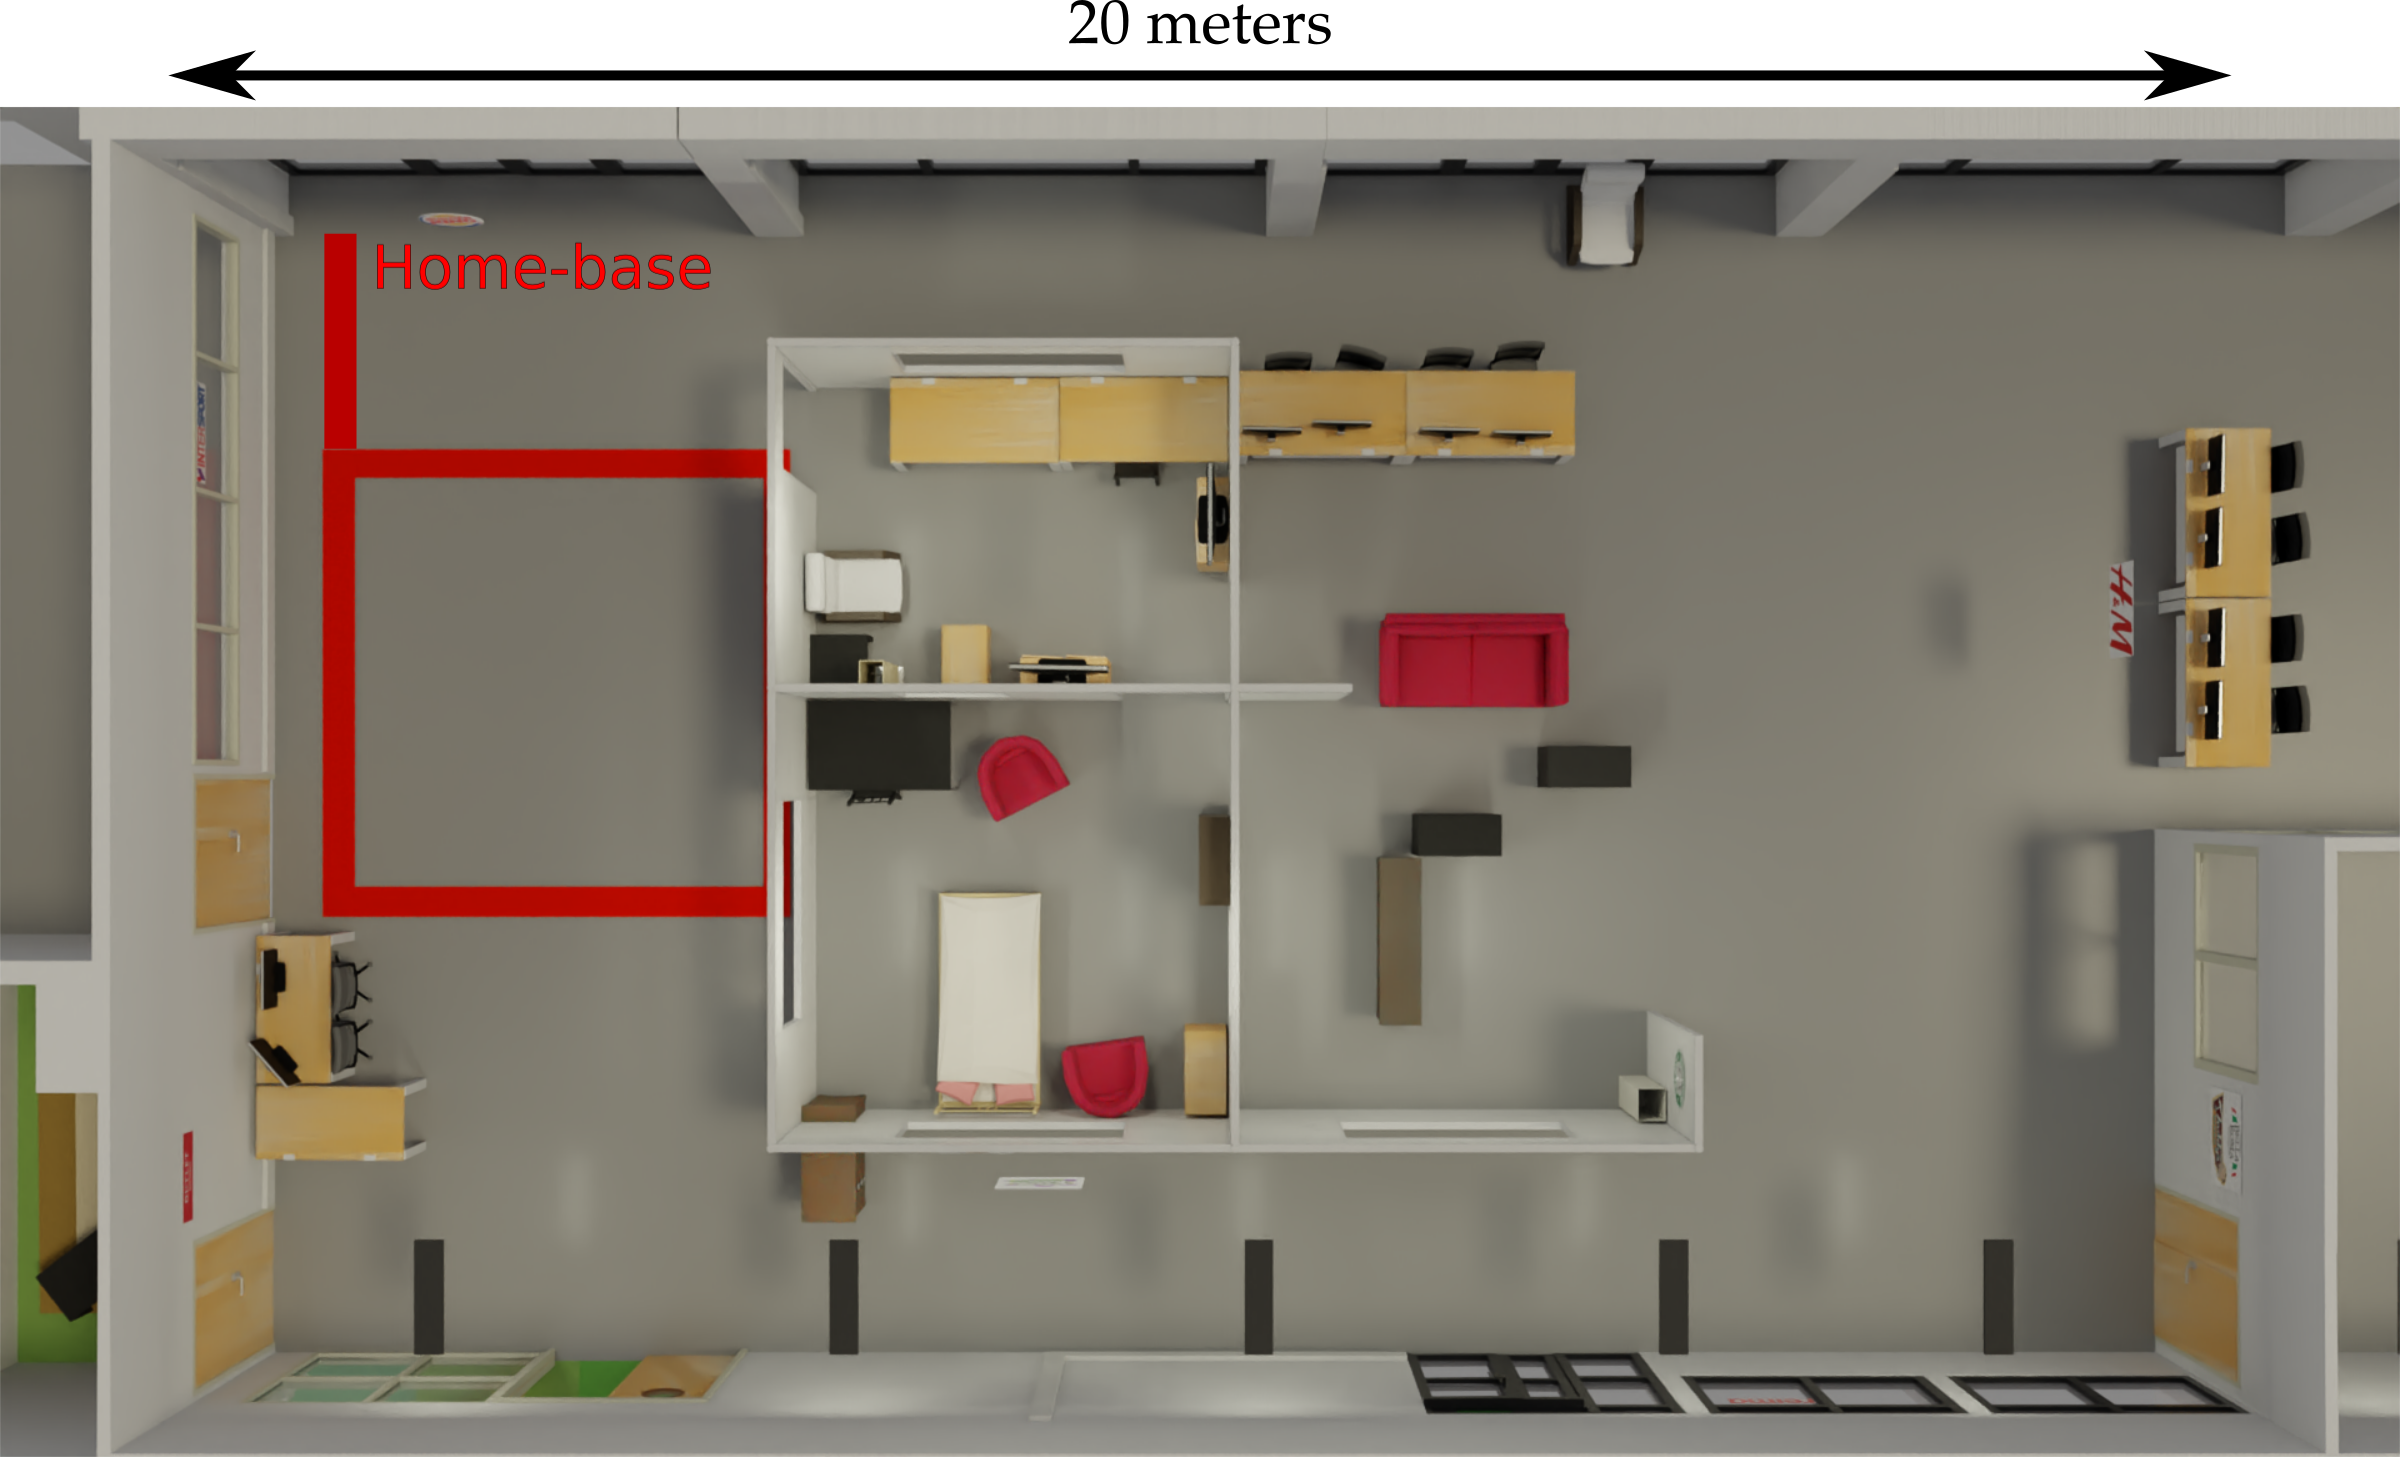
\includegraphics[scale=0.15]{figures/chapter3/adream_base_m.png}}
	\end{subfloat}
	\begin{subfloat}[The 3D mesh model of the real mall in Finland. The entire mall having a size of 528.6 meters per 247.5 meters on two levels, we have only modelled the part which can be visible from the interaction area. It results in a model of 150 meters per 69 meters.\label{fig:chap3_ideapark}]{
			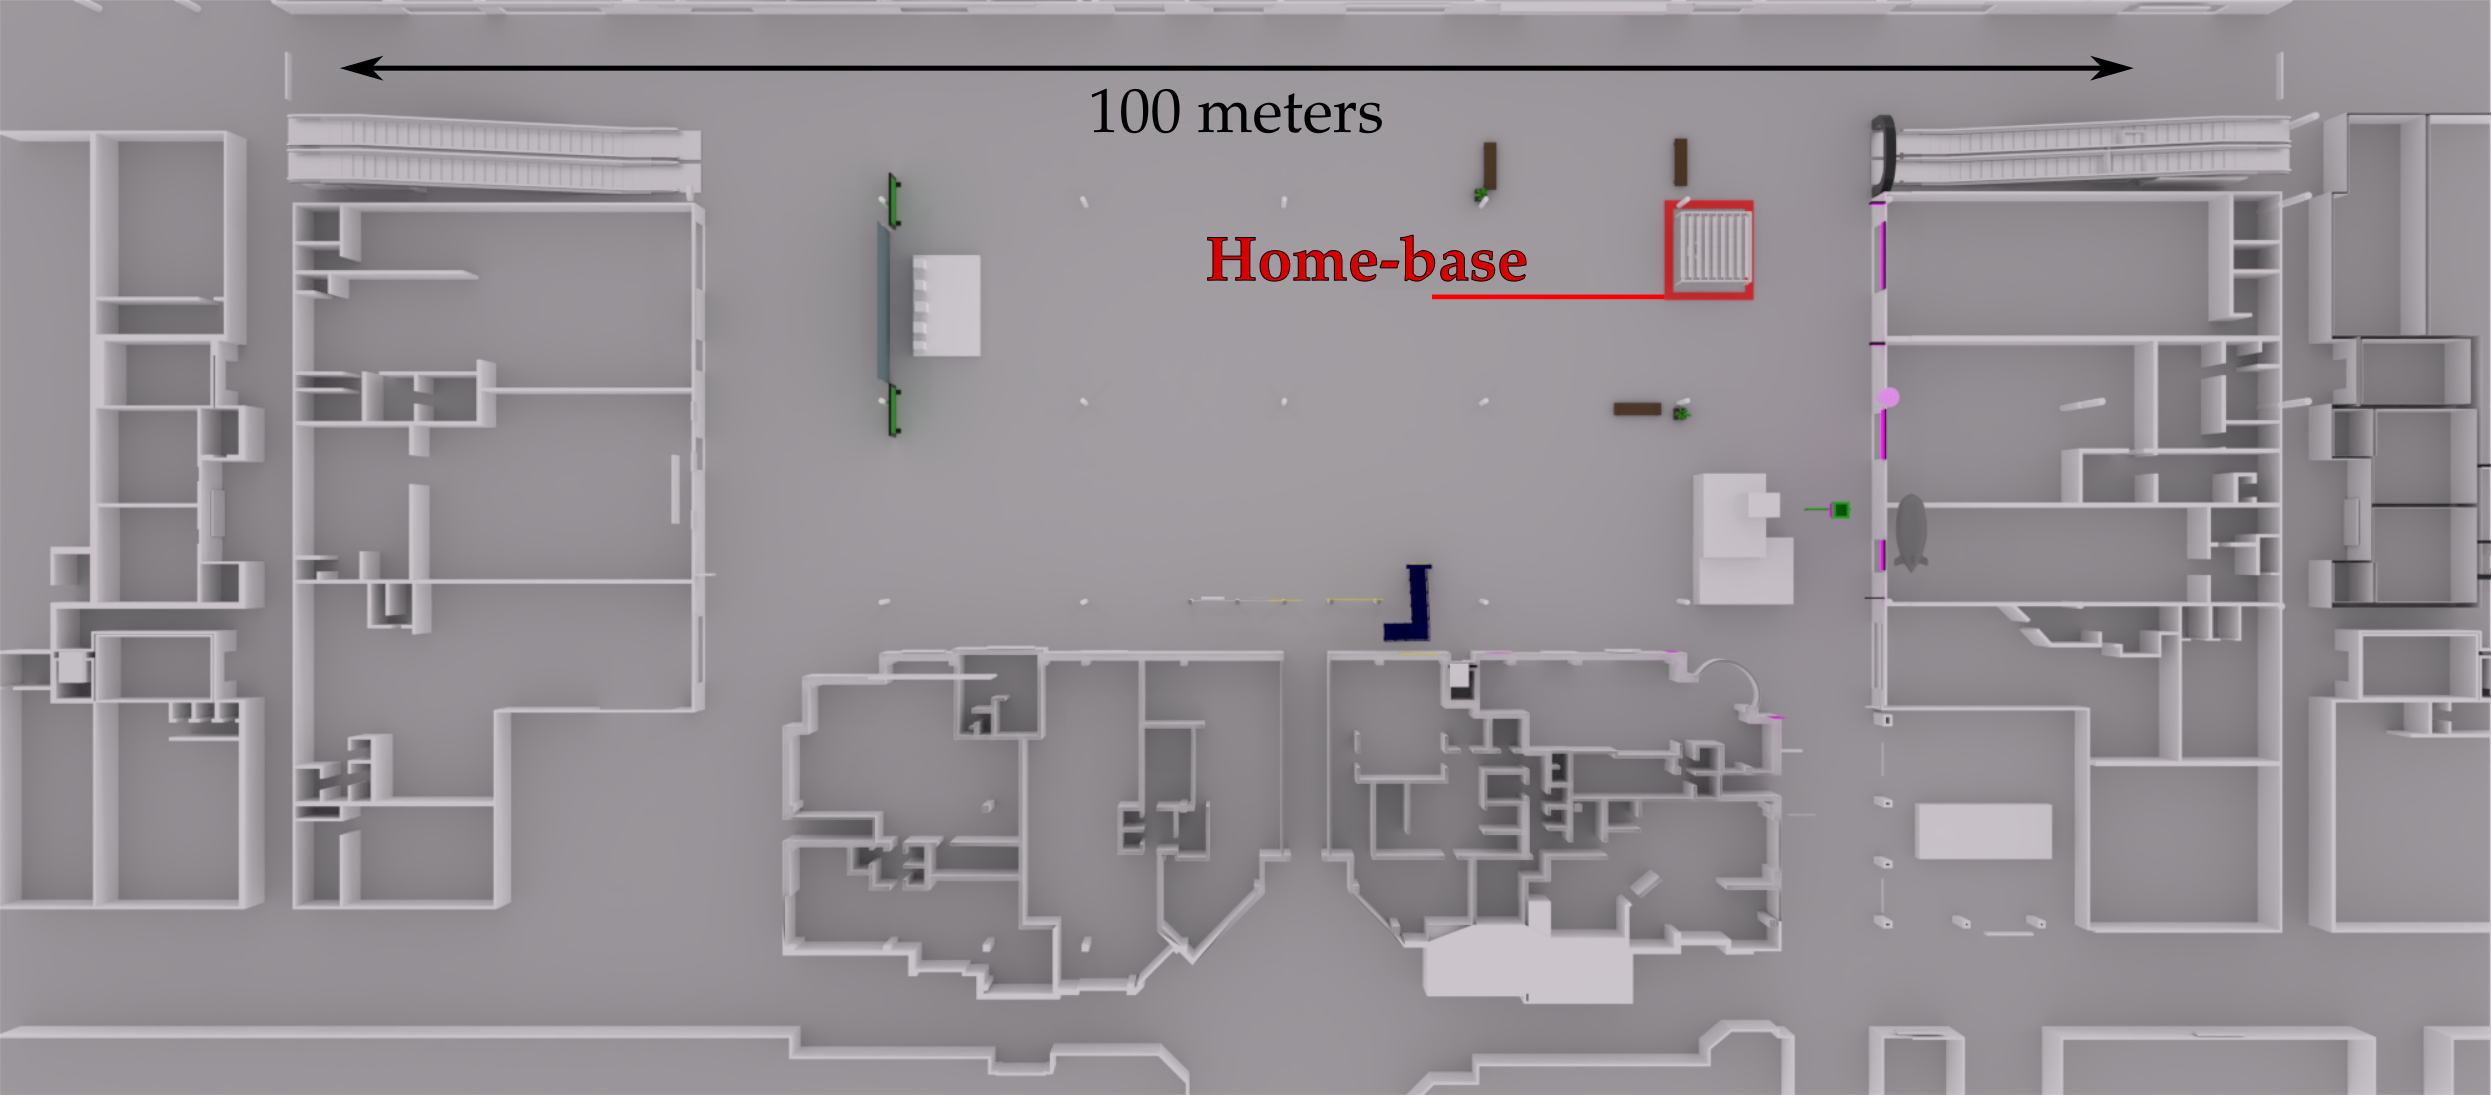
\includegraphics[scale=0.15]{figures/chapter3/ideapark_base_m.png}}
	\end{subfloat}
	\caption{We have built a mockup of the Finnish mall environment in our lab in order to be able to test and debug the direction-giving task in our lab. This environment comprises a two-level area with corridors, ``shops'' , passages, stairs, open central space and consequently allowed us to run realistic guiding scenarios.}
	\label{fig:chap3_3Dmodels}
\end{figure} 


In order for the pointing planner to compute the visibility of the landmarks used for the route description, stairs, escalators, elevators, and store signs are represented each by a single mesh while the rest of the building is a unique 3D mesh. This means that a store is said to be visible if we can see its sign, which we think to be the most relevant element to see to recognize a shop.

The 3D model is also used to generate a navigation map, constraining the robot to move in the interaction area while avoiding obstacles in it.

\subsubsection{Semantic representation}\label{subsubsec:semantic}

As \cite{satake_2015_field}, our semantic representation is based on ontology. An ontology allows to define classes representing general concepts (e.g. Restaurant), individuals/entities being classes instantiations (e.g. Burger\_King), and properties linking two entities (e.g. Burger\_King isIn Ideapark).
To provide storage and an efficient way to manipulate the ontology and reason about it, a lightweight software has been developed, called Ontologenius, presented by \cite{sarthou_2019_ontologenius}. It makes it possible to share the semantic knowledge among all the components of the architecture, here especially the route handler and the supervision, thus enabling a unique repository of knowledge.

The ontology is first used to represent information about the stores. It allows to define and refine the shared goal of the task by understanding the client's wanted destination. Thus, the stores' types, their names, and the items they sell have been represented in it with a rich semantic. It allows for example to represent that both soda and hamburgers are sold in fast-foods, which are types of restaurants, but that soda can also be found in a supermarket. Thanks to Ontologenius, the names of concepts are defined in different languages and with synonyms for these names. It allows the robot to adapt itself to the human partner language. Moreover, Ontologenius endows the robot with the ability to recognize a set of names in natural language but that it will be prevented to use (e.g. the robot can understand a reference to ``bank'' when a human says it but only refers to it as ``ATM'' or ``cash machine'' since there was no bank office in the mall). In addition, this software offers a fuzzy match service based on Levenshtein distance, to help the supervision system to handle ambiguities coming from the speech to text component (e.g. it can match the word ``Juwelsport'' with ``Juvesport''). This set of functionalities around the concepts' names facilitates the understanding of the partner's need and thus helps at increasing the quality of interaction.

In an effort to unify representations because representing as a 3D mesh the entire mall would be a complex task, we chose not to use the geometrical representation or a topological map to compute the route to the final goal but rather the semantic representation given by the ontology.

To include topological information into the semantic representation, the \acrfull{ssr} has been designed, presented by \cite{sarthou_2019_semantic}. With the \acrshort{ssr}, the overall knowledge is represented in an ontology with three upper classes which are: \textbf{region} (\ie a two-dimensional area that is a subset of the overall environment), \textbf{path} (\ie a one-dimensional element along which it is possible to move and which has a direction) and \textbf{place} (\ie a point of zero dimension that can represent a physical or symbolic element). The \textbf{place} class has three subclasses: \textbf{path intersection} (\ie the connection between only two paths and thus a waypoint to go from one path to another), \textbf{passage} (\ie the connection between only two regions and thus a waypoint to move from one region to another like a door, a staircase or a passage), and \textbf{shops}. A representation of these classes is visible in Figure~\ref{fig:chap3_onto_classes}.

\begin{figure}[!ht]
	\centering
	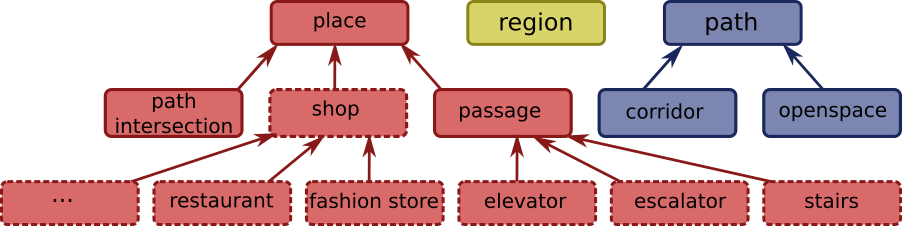
\includegraphics[scale=0.45]{figures/chapter3/classes.png}
	\caption{\label{fig:chap3_onto_classes} Classes for a representation of the topology of an indoor environment in a semantic description. The classes with the solid outline are the minimum classes defined by the \acrshort{ssr}. The classes with the dotted outline are an extension of this minimal set.}
\end{figure}

An example of the final semantic knowledge represented in the ontology for a given shop is presented in Figure~\ref{fig:chap3_onto_properties}. We find here the identifier of the shop, the category to which each store belongs (e.g. restaurant or hairdresser), the items sold for which people ask the most (e.g. shoes or coat), and the names and synonyms in natural language and that for different languages.
Moreover, thanks to the \acrshort{ssr} we can produce the best route (in term of complexity) as well as verbalize it using a route perspective.

\begin{figure}[!ht]
	\centering
	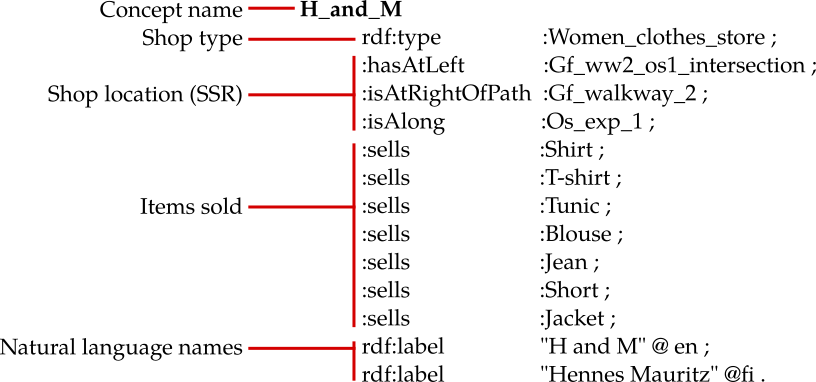
\includegraphics[scale=0.45]{figures/chapter3/zizzi.png}
	\caption{\label{fig:chap3_onto_properties} Properties for a representation of the topology of an indoor environment in a semantic description.}
\end{figure}

\subsection{Perceiving the partner}\label{subsec:situation_assessment}

The situation assessment component is based on the Underworld framework~\cite{lemaignan_2018_underworlds}. It aims at gathering perception information in the form of 3D position and orientation of human faces, with the 3D model and the robot state. With this information, it is able to generate the symbolics facts listed in table~\ref{tab:chap3_predicates}.

\begin{table}[ht!]
	\centering
	\begin{tabularx}{\textwidth}{|l|X|}
		\hline
		\textbf{Predicate} & \textbf{Description} \\
		\hline
		\hline
		isPerceiving & The robot is perceiving a human \\
		\hline
		isCloseTo & The human is within a distance of 0 to 1 meter of the robot \\
		\hline
		isLookingAt & The human is looking at the robot \\
		\hline
		\hline
		isInArea & The human is in the interaction area \\
		\hline
		isEngagingWith & The human is close to the robot and is looking at it \\
		\hline
	\end{tabularx}
	\caption{Facts computed and monitored during the direction-giving task.}
	\label{tab:chap3_predicates}
\end{table}

\subsection{Managing the robot's resources}

A humanoid robot such as Pepper can be seen as a composition of multiple physical components that can act independently of each other. For the pointing task, we identified four resources: the head, both arms, and the base. At the beginning of the interaction, for example, the head is used to find people to interact with, but later it will be used to track the human with the gaze. Several components could access this resource to perform these actions. However, they do not have a global picture of the ongoing task. In this case, a resource could be used by several components at the time. Consequently, it could lead to task failures.

Moreover, in some cases, several resources have to be used simultaneously to perform a high-level action. To point to a landmark, one arm is selected to point while the other has to be lowered. The base is then rotated if the arm reaches the joint limit to point a target on its back. If at least one of the involved resources is simultaneously used to perform another action, the overall high-level action will fail as the global posture will no more be clear. For example, if the human gets too close to the robot and a component tries to move away from a little, the arm would no more point in the right direction.

Thus, the correct handling of all the resources is critical for performing the task, but it can be cumbersome for a deliberative component, such as the Supervision, to do all the micro-management required. To tackle this issue, a physical resource management system has been designed by Guillaume Sarthou and Guilhem Buisan. For each of the identified resources is instantiated a component called \textbf{Resource Manager}, having two types of input: permanent commands that can be preempted at any time (e.g. look at the head of the human interacting with it) and finite state machines which are not preemptable (e.g. set of commands to point). A component called \textbf{Resource Synchronizer} deals with actions requiring multiple resources such as the human-aware navigation which uses the head and the base. The synchronizer also reports the status of the ongoing coordination signal to the Supervisor to monitor the progress of the action. Finally, a priority scheme has been implemented to handle multiple active inputs at the same time for one resource. 

The global resource management scheme is illustrated in Figure~\ref{fig:chap3_rm} with four resource managers and one synchronizer.

\begin{figure}[!hb]
	\centering
	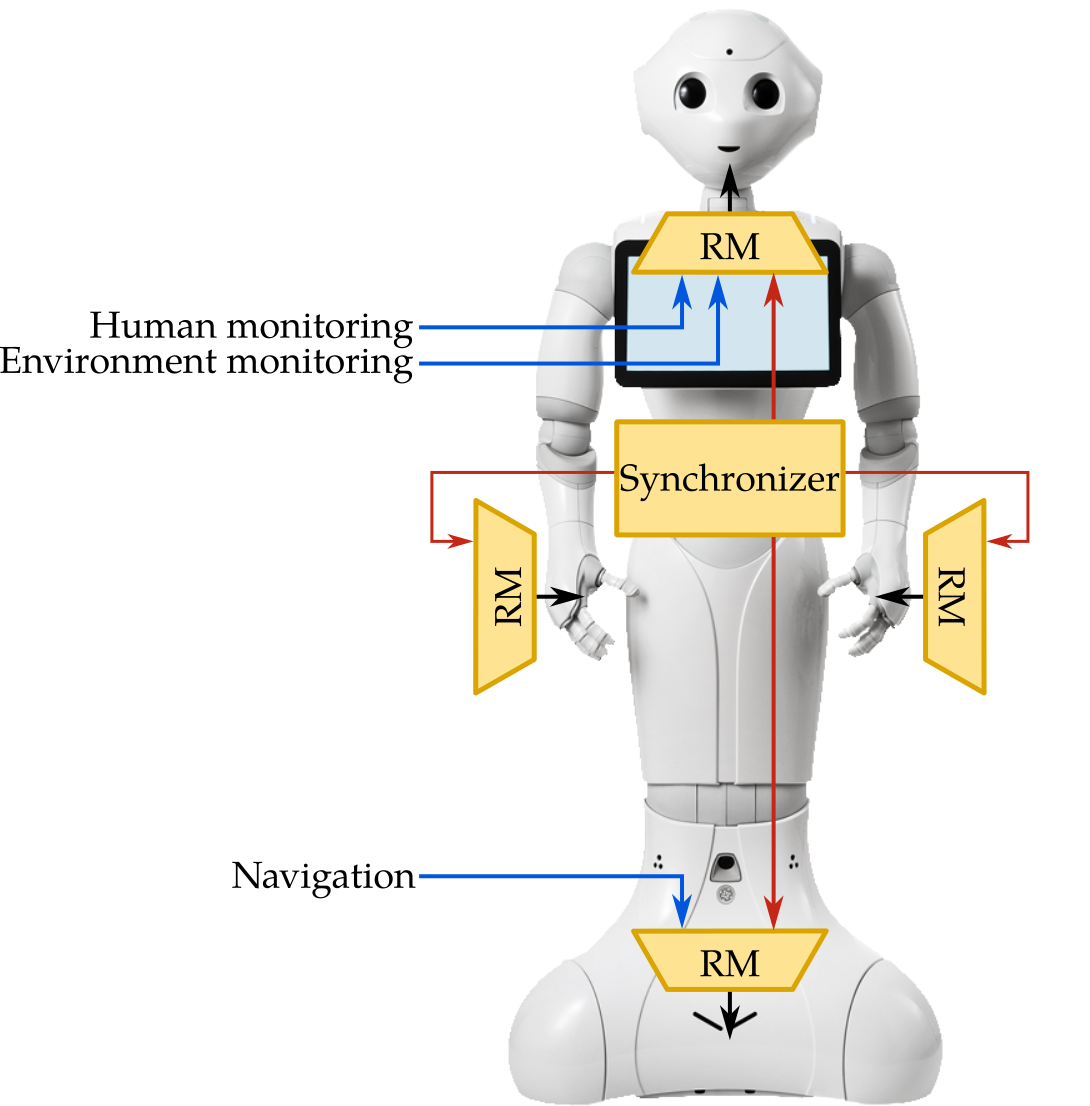
\includegraphics[scale=0.26]{figures/chapter3/rm.png}
	\caption{\label{fig:chap3_rm} Representation of the resource management system with four resource managers and a synchronizer. The red arrows represent the state machines inputs and the blue arrows represent the inputs for permanent commands.}
\end{figure}

\subsection{Describing the route to follow}\label{subsec:route_description}

In large-scale environments such as malls, route computation can lead to combinatorial explosion. Therefore, to simplify the problem we chose to divide it in two stages and to conceive an algorithm for each one. The first one computes the existing routes from one Region of the mall to another. A region is for example a floor of the building so if the robot is at the ground floor and the final destination also, this means that the algorithm will not take into account all the elements of the other floors. Then, the second algorithm uses the Region-to-Region routes to calculate the Place-to-Place route. These algorithms are presented with more details in \cite{sarthou_2019_semantic}.

\paragraph{Region-to-Region route}

\begin{figure}[b]
	\centering
	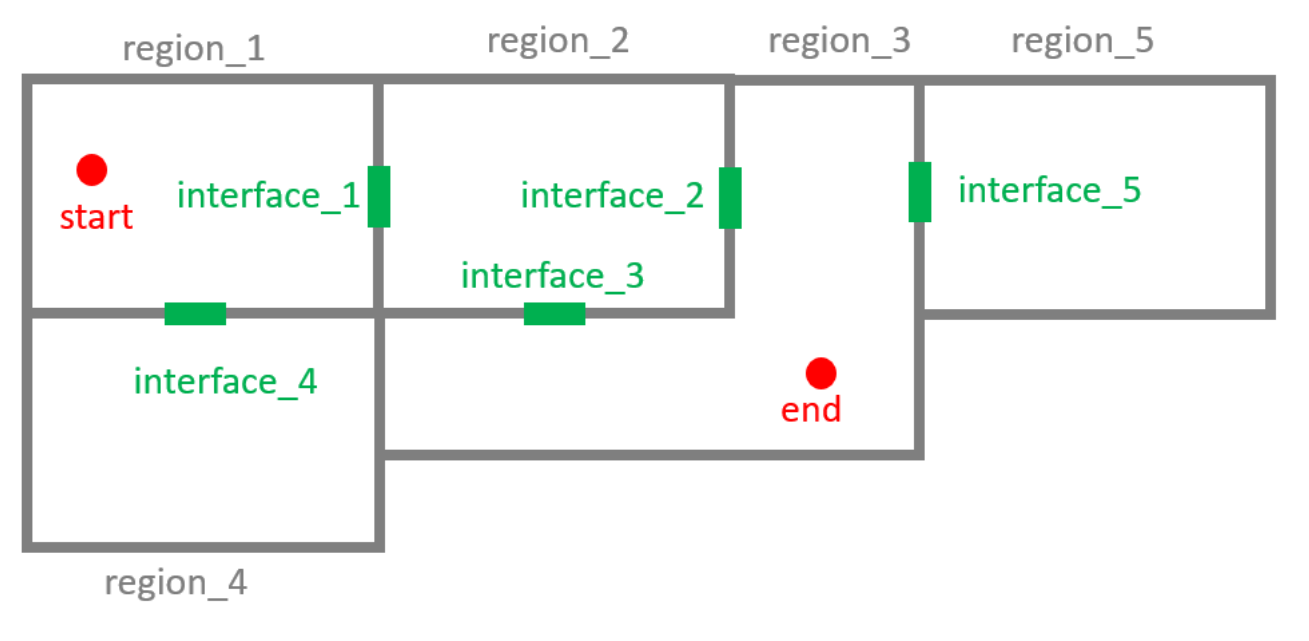
\includegraphics[scale=0.17]{figures/chapter3/regions.png}
	\caption{\label{fig:chap3_regions} Representation of an environment at the regional level.}
\end{figure}

In the \acrshort{ssr}, \textbf{passages} (e.g. escalators, stairs) are elements of the environment connecting two regions through the $isIn$ property. With this property and a breadth-first search algorithm, Region-to-Region route finding algorithm is able to find the routes connecting two regions using only passages. It outputs a route with the format $region - place - region - ... - region$. In the example of Figure~\ref{fig:chap3_regions}, the final routes found by the algorithm to go from Region 1 to Region 3 are:

\begin{itemize}
	\item \(region\_1 - passage\_1 - region\_2 - passage\_2 - region\_3\)
	\item \(region\_1 - passage\_1 - region\_2 - passage\_3 - region\_3\)
\end{itemize}


\paragraph{Place-to-Place route}

The Place-to-Place route search is based on the Region-level search results. It decomposes each route into sub-routes of the form $place - region - place$. In our example, the division gives five unique sub-routes:
\begin{itemize}
	\item \(start - region 1 - passage\_1\)
	\item \(passage\_1 - region\_2 - passage\_2\)
	\item \(passage\_2 - region\_3 - end\)
	\item \(passage\_1 - region\_2 - passage\_3\)
	\item \(passage\_3 - region\_3 - end\)
\end{itemize}

Then, the algorithm aims to replace each sub-route region with a succession of paths and intersections. It works on the same principle as the previous search algorithm using the $isAlong$ property instead of the $isIn$ property. Still taking the same example and focusing on $region\_1$, it can solve the sub-route \( start - region\_1 - passage\_1\). $Region\_1$ is represented with its corridors and intersections in Figure~\ref{fig:chap3_region_1}. By applying the breadth-first search algorithm at the Place level, a solution of the form $place - path - place - ... - place$ is obtained. So for our example, \(start - corridor\_1 - intersection\_1 - corridor\_5 - passage\_1\) is a solution for the first sub-route. By doing the same for each sub-route, we can then recompose the global routes and give a detailed set of routes from start to end.

The second place of the route -- the third element of the route objects -- is the one we call the passage in the description of the direction-giving task, the first salient landmark of the route to point to, which is on the way to reach the final place, \ie \(intersection\_1\) in the example.

\begin{figure}[ht]
	\centering
	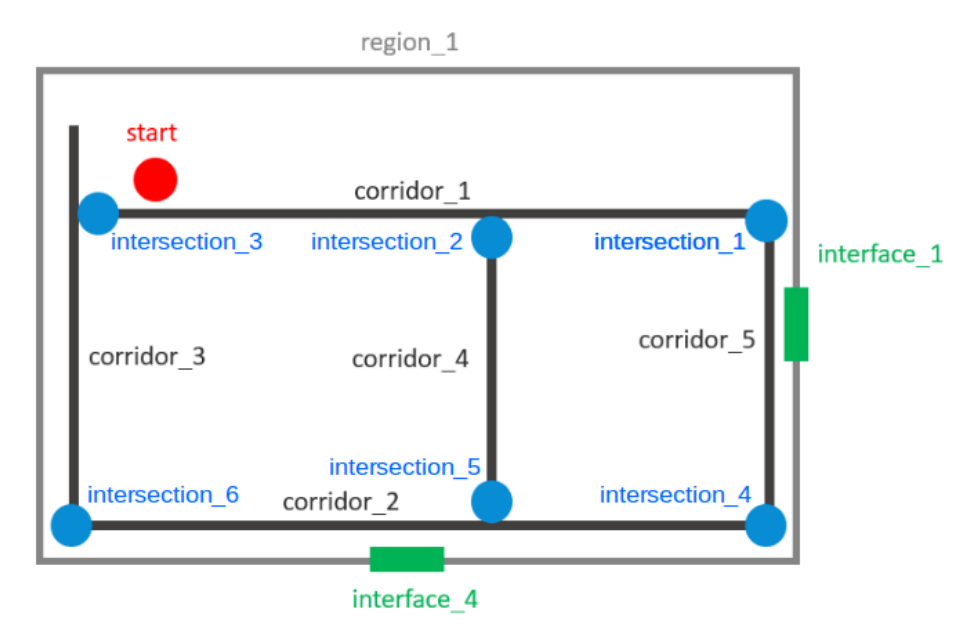
\includegraphics[scale=0.25]{figures/chapter3/region_1.png}
	\caption{\label{fig:chap3_region_1} Representation of corridors and intersections in region\_1}
\end{figure}

\subsection{Planning a shared visual perspective}\label{subsec:svp}

When the robot has to point to a target, two criteria have to be respected. First, the human has to be able to see the target. Second, the human has to be able to look at the pointed target and at the robot without turning the head too much. It goes the same for the robot as it has to see the pointed target, meaning not to point toward a wall and be able to simultaneously point at the target and look at the human. Consequently, to point a target in its back, it has to move. The robot and the human can thus move in the interaction area during the direction-giving task, to move to a better position for pointing at the target. To find the robot and human possible positions we designed a component called the SVP (Shared Visual Perspective) Planner, presented in~\cite{waldhart_2019_reasoning}. For the purpose of the deployment, the presented version is an adapted and slightly simplified version.

To compute the visibility of both agents, the planner has access to the geometrical representation of the environment and the agents current positions. In addition, it considers an estimated agent's maximal speed to move and a visibility threshold.

When the robot explains the route to the human and points to a landmark, they form what is called an F-formation. Kendon explains that \textit{``An F-formation arises whenever two or more people sustain a spatial and orientational relationship in which the space between them is one to which they have equal, direct and exclusive access''} \cite{kendon_1990_conducting}.
This F-formation has been decomposed in \cite{mcneill_2005_gesture} into two types: the social formation and the instrumental formation. While the first type corresponds to the original definition, the instrumental formation includes a physical object that all the agents can gaze at. This means that once the robot will have moved, the human will come in front of it creating a social formation in the form of a vis-a-vis (each facing the other) and when the robot will point they will change for an instrumental formation. Indeed, when both agents will reach their position computed by the planner, we want them to be able to go from one formation to the other with only a rotation; the human will not need to move again from their arriving position to see what the robot will point. 

To search for better positions to reach in order to point a landmark, the planner takes three main parameters into account:

\begin{itemize}
	\item Visibility constraint: The two agents can see either the target shop when it is the only element of the route or the passage.
	\item Navigation distance cost: The agents do not have to move too much.
	\item F-formation cost: The human-robot-target angle and a robot-human-target have to be less than 90${^\circ}$. 
\end{itemize}

\begin{figure}[ht!]
	\centering
	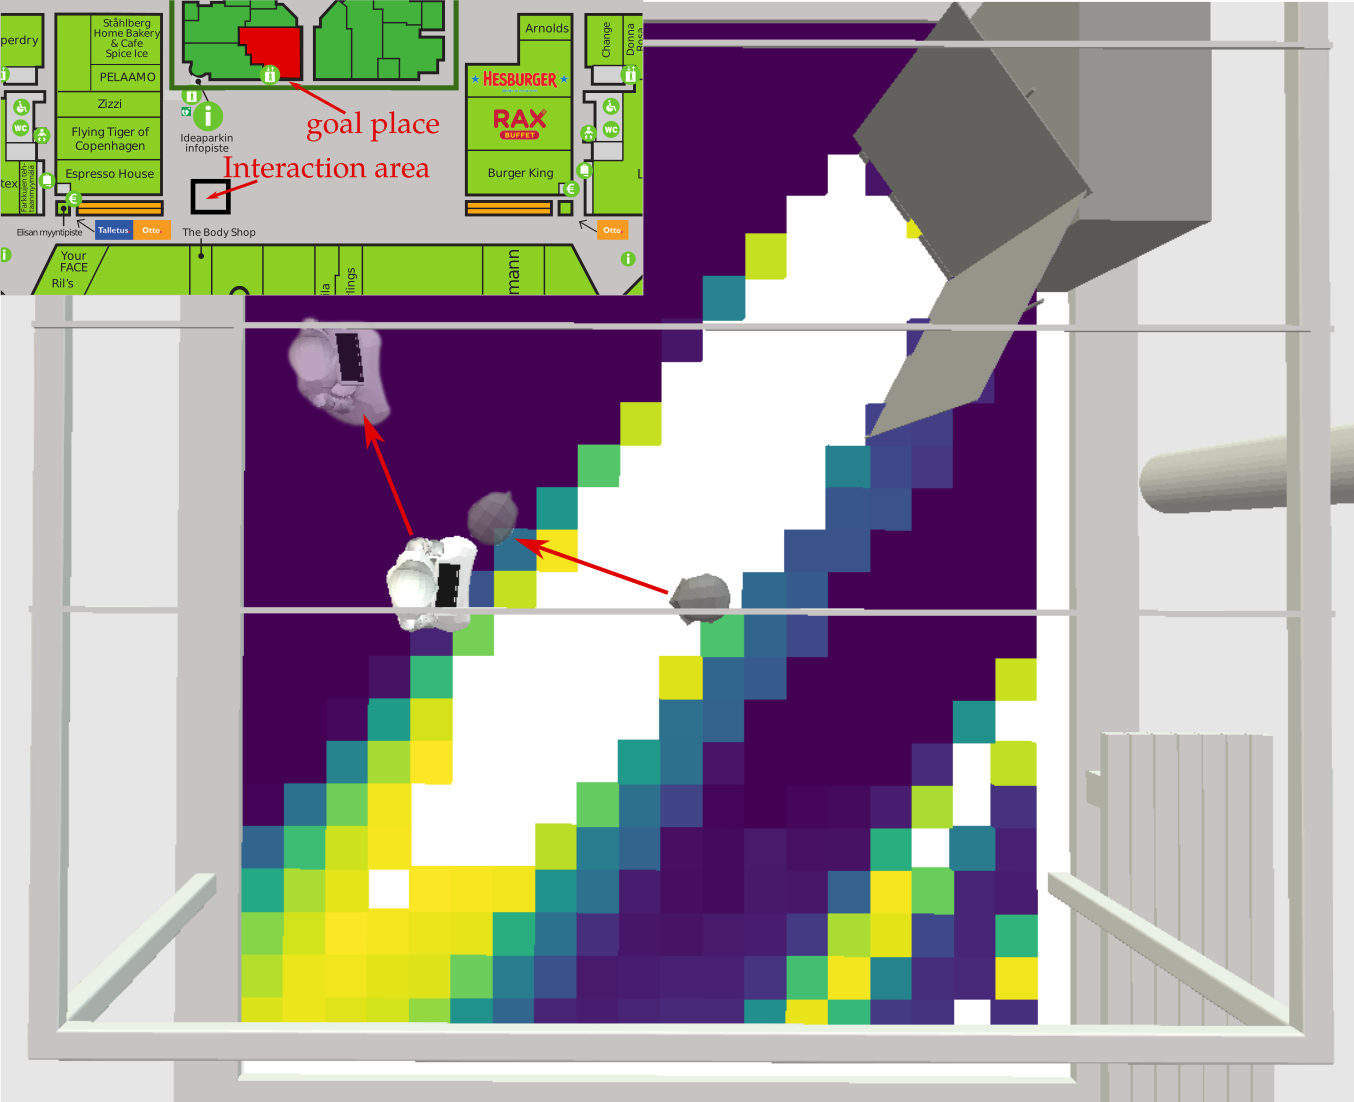
\includegraphics[scale=0.3]{figures/chapter3/grid_map.png}
	\caption{\label{fig:chap3_svp_grid} Visibility grid for a target located at the top right. The uncoloured areas represent an absence of visibility and the others represent the cost of visibility ranging from yellow for low visibility to purple for good visibility. The robot and the human in transparency on the image represent the final calculated positions while the others are the initial positions. }
\end{figure}

To compute the positions, the interaction area is firstly decomposed into a weighted three-dimensional (x,y for the possible positions in the area and z for the human height) grid representing the estimated human visibility of the target. The target visibility is computed offline for each position of the grid. It is based on the part that the target takes in the 360${^\circ}$ field of view of the environment. Such grid is represented in figure~\ref{fig:chap3_svp_grid} for a given human height. The white cells are positions from which the human cannot see the pointed target. The other colored cells represent the degree of visibility from the poor in yellow to the good in purple. Having the human visibility grid, the goal position is computed using a weighted cost function between good visibility and restricted distance to cross. In the example of figure~\ref{fig:chap3_svp_grid}, the transparent human head is the human goal position while the other is the initial position. From the initial position, the human was not able to the pointed target. 

The robot position is computed in a second time, according to the human planned position. Divided the search into two steps allows reducing the search complexity. The robot position is thus constrained by the human one. It has also to respect a minimal and maximal distance to the human and minimal visibility of the target from it. Finally, the robot position is also determined regarding a cost preferring an F-formation limiting the robot reorientation, meaning that it can point to the target keeping its torso and its chest oriented towards the human.


\subsection{Navigate close to human}\label{subsec:navigation}

The Human-Aware Navigation component aims at moving the robot while avoiding dynamic and static obstacles in addition to proposing a socially acceptable navigation solution for the robot. For example, the robot should not pass too close to the human and should not show its back while navigating around the human. A full presentation of the planner is available in~\cite{singamaneni_2020_hateb}.

\subsection{Robot execution control and supervision in a joint action context}\label{subsec:supervision}

subsubsection{A supervision and control system dedicated to human-robot joint tasks}
A service robot interacting with humans in a mall and providing directions to them needs a number of abilities to enable a smooth and efficient interaction. As explained in Section~\ref{sec:rationale}, the direction giving task is an asymmetric joint action, with the robot in the guide role and the human in the guided role. The \textit{Supervisor}, the supervision and control system of the robot, is built taking this specificity into account, embedding a shared representation of the direction giving task. More specifically, when giving directions to a human, the robot plans its actions and the human ones and then execute its part of the plan. To be able to know if and when the human performs their actions, it monitors the action executions and interpret the information received from the Situation Assessment (see Section~\ref{subsec:situation_assessment}). Furthermore, in such interaction, communication is important, thus the robot communicates verbally as well as non-verbally, and listens to the human. All along the interaction, it needs to maintain a distinct mental state model for the human and itself concerning the knowledge of both agents and the state of the world. Finally, it should be able to tackle events and contingencies happening during the task and to drop it when necessary.

\todo{voir lien avec chapter 1}
%The Supervisor manages the robot's interactions with humans on three levels: \textit{interaction sessions}, \textit{direction-giving task} and \textit{actions}. We defined an \textit{interaction session} as the period during which the robot and a human interact together and are engaged. It is divided in three parts, following the structure proposed by~\cite{sidnell_overall_2012} and the engagement model of~\cite{sidner_2003_engagement}: the \textit{greetings}, the \textit{body of the interaction} and the \textit{goodbyes}. 
%During an interaction session, 
%in this implementation, the human and the robot can chat, play a quiz, and perform direction-giving tasks. The layers of an interaction, each of them also representing a level of decision for the Supervisor, are modelled in Figure~\ref{fig:session}. 
A \textit{direction-giving task} occurs when the human involved in the ongoing interaction session asks for directions to a place or for locations of sold items. 
% The robot, if necessary, refines the human goal, establishes a shared goal~\cite{cohen1991}, enquires about their willingness and abilities of climbing stairs, updates its estimation of the human mental state. Then, it gives route directions while pointing at landmarks, taking their perspective into account for the landmark and the route. Finally, it checks if it has been understood, making sure that the person has all the information to complete the shared goal, being the human reaching its destination. The robot executes all these steps thanks to \textit{actions}, communicative ones or on the environment.

%\begin{figure}
%    \centering
%    \includegraphics[width=0.9\linewidth]{figures/chapter3/session_interaction.png}
%    \caption{Representation of the interaction session and the task levels. For each of them, the Supervisor has a decision-making process.}
%    \label{fig:session}
%\end{figure}
\todo{voir lien avec chapter 1}
%\subsubsection{Selecting a framework for a Supervisor dedicated to the joint action}
%To implement the Supervisor, we chose a framework among the different existing ones dedicated to supervision and execution. We compared existing open-source decision-making and execution software. To cite a few, there is the PetriNetPlans library introduced by~\cite{ziparo2011} which is a framework for planning and execution. \cite{beetz2010} developed CRAM, a software implementing reasoning mechanisms that can infer control decisions. Finally, our choice went to Jason designed by~\cite{bordini_2007_jason} which is a Java interpreter of AgentSpeak created by~\cite{rao1996}. Compared to the other software, it has the advantage to be a BDI (Beliefs, Desires, Intentions) agent-oriented framework, fitting with our architecture. As mentioned previously, BDI frameworks are primarily focused on practical reasoning, \ie the process of deciding, step by step, which action to perform to reach a goal. It allows more modularity than state machines to handle contingencies and events. It also facilitates reasoning on agents' -- humans and robot -- beliefs.
%
%\subsubsection{Implementation of interaction sessions}
%An interaction session is triggered when a human $human_i$ is close enough to start a conversation and seems willing to (\ie when the Supervisor receives the predicate isEngagedWith($human_i$, $robot$) from the Situation Assessment, in this way, the robot tries to respect people that does not want to interact with it. From there, the robot is in the first phase of the interaction session, the \textit{greetings}. The robot says hello to the human and announces the activities it can perform with them: to give directions, to chat, and to play a quiz\footnote{Chat and quiz activities are handled by the Heriott-Watt University (HWU) Dialogue component, there are out of the scope of this paper.}. From this moment, the Supervisor orders the Physical Resources Manager (see Section~\ref{sec:head_management}) to make the robot's head tracks the human's head. This tracking has two purposes: to signal its engagement and to monitor the human's actions. This behavior is quite similar to the one described by~\cite{satake_what_2015}. 
%
%The interaction session stays open as long as the human and the robot perform activities together, \ie as long as the human is engaged in the interaction. This engagement is monitored by the robot in different ways: through the predicate isEngagedWith($human_i$, $robot$) during information exchange phases and through action results when an action is to execute. If at some point the human is not perceived for a while -- the Supervisor did not receive from the Situation Assessment the predicate isPerceiving(\(robot, human_i\)) for more than 6 seconds -- or the human says goodbye, then the Supervisor ends the session. In the latter case, the robot replies with goodbyes. Also, the Supervisor signals the Physical Resource Manager to stop tracking them. Finally, the Supervisor makes the robot return to its starting point and launch the re-localization process.
%(see Section~\ref{subsubsec:nav:loc}).

\subsubsection{Implementation of the direction-giving task and its associated actions}\label{subsubsec:sup:subtasks}
\begin{figure}[hbtp]
	\centering
	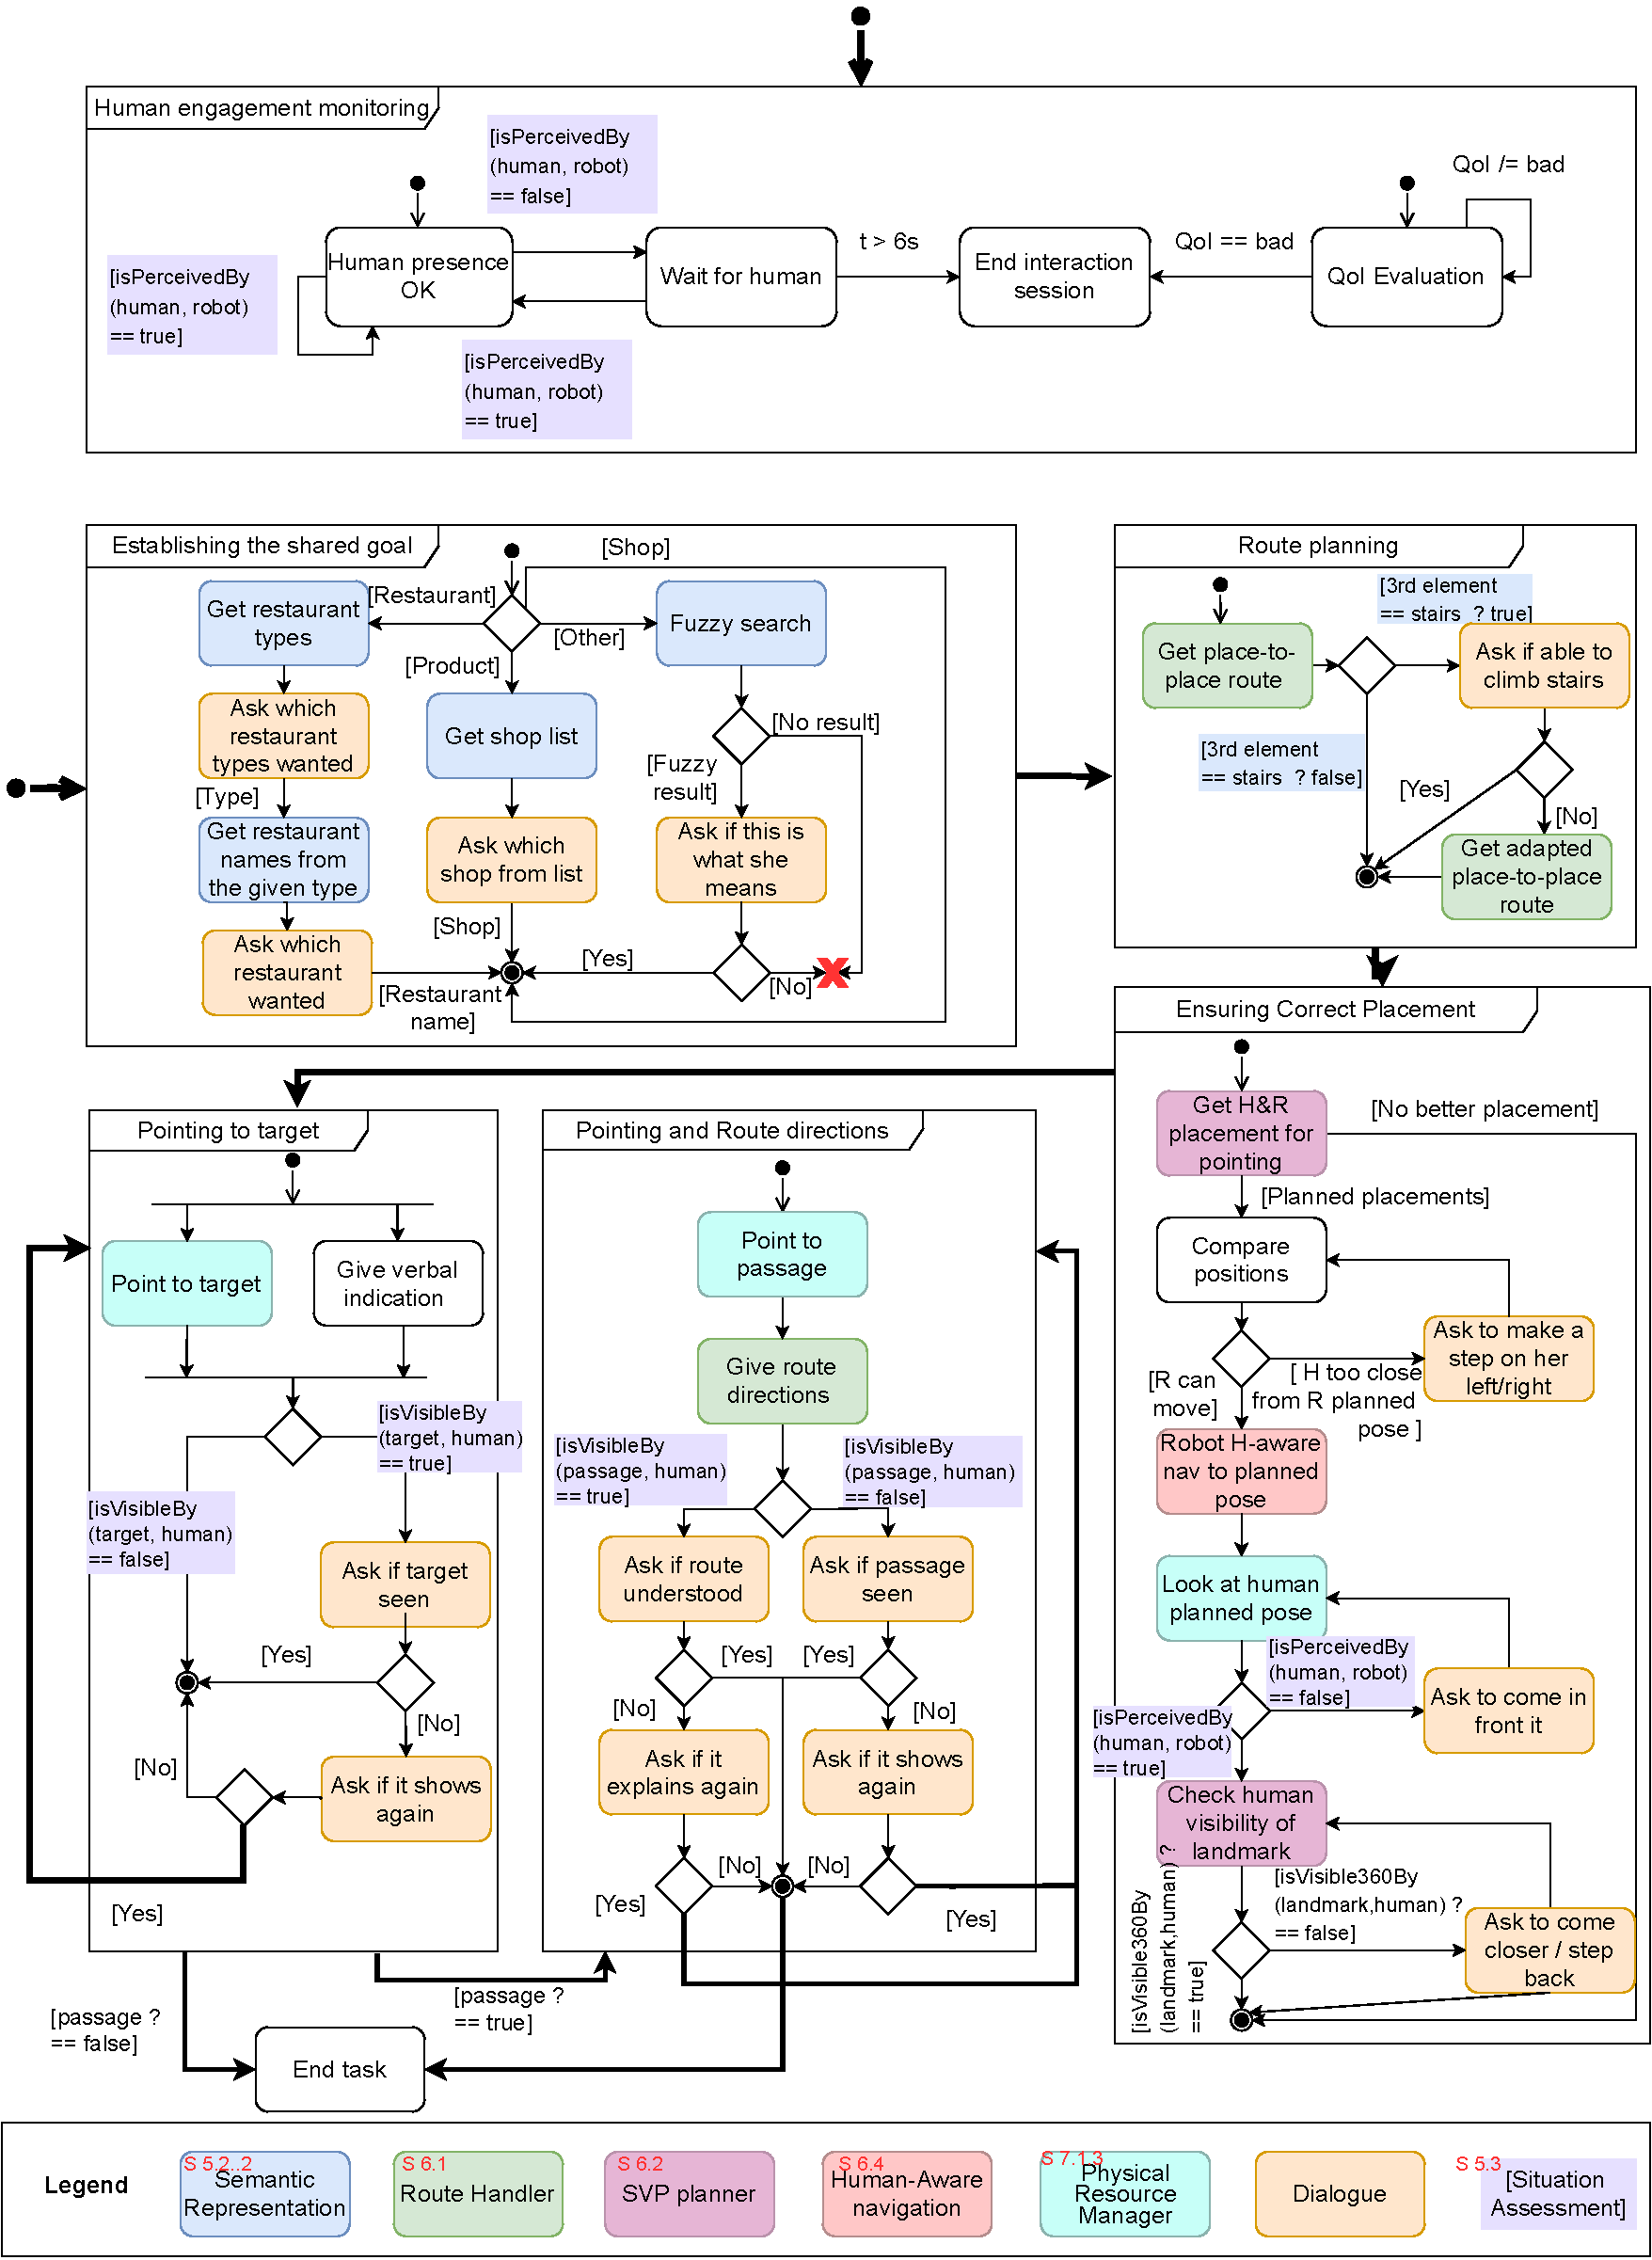
\includegraphics[width=\linewidth]{figures/chapter3/state_machines.pdf}
	\caption{\label{fig:chap3_SM} Supervisor activity diagram of the direction-giving task. Each action has a color corresponding to the component with which the Supervisor interacts to execute it. It goes through every subtasks described in Section~\ref{subsubsec:sup:subtasks}. Also, the human engagement monitoring is represented. Texts between brackets correspond to beliefs on which depends the decision-making process. These beliefs can either be provided by other components or being the result of the Supervisor's own computations. }
\end{figure}

The Supervisor can be seen as a puppet master. It manages the robot's decisions of when to act, what to say, and what to do during the task. It decides, executes, and supervises the proceedings of the execution as well as the human actions, using and coordinating all the other components of the architecture at its disposal.

The Supervisor is implemented using Jason, so it can manipulate beliefs and reactive plans (written offline by the developer rather than planned during the interaction). For the interaction session and the direction-giving task, at execution time, plans are chosen among the ones from the plan library when triggered by an event or by another plan. The same plan can have multiple versions and the version to be executed is selected according to the pre-conditions (also called context). For instance, the plan \textit{verbalization(Target)} has two different versions, one in the case where the target to point is visible and the other one in the case where it is not, and at execution time, the selected one will depend on the presence or not of the belief \texttt{visible\_target(Target)} in the Supervisor belief base, as shown in Listing \ref{listing:plan}:

\begin{lstlisting}[caption = Two different plans for \texttt{verbalization(Target)}, label = {listing:plan}]
+!verbalization(Target)                 // plan name
: visible_target(Target)            // context
<-  ?verba_name(Target, Name);      // belief query
say(visible_target(Name)).      // action

+!verbalization(Target) 
: not visible_target(Target)
<-  ?verba_name(Target, Name);
say(not_visible_target(Name)).
\end{lstlisting}

Even though the direction-giving task is implemented with reactive plans, it can still be represented with an activity diagram, for presentation purposes. This activity diagram is visible in Figure~\ref{fig:chap3_SM}. Each frame represents one of the steps described in Section~\ref{sec:guiding}. We now present their internal functioning and the interactions with the multiple components of the system the Supervisor has.

\paragraph{Establishing the shared goal}
When a person triggers a direction-giving task, they might directly ask something like ``where is the pharmacy?'' which allows the robot to directly establish the shared goal but, they might also ask something less precise. In the latter case, the robot needs to inquire about the human desired place to reach in order to establish the shared goal\todo{reminder def}.

When a person asks ``Where is a good restaurant?'', the robot presents a list of the types of food available, namely ``There are casual dining restaurants, Asian restaurants, native food restaurants, hamburger restaurants, fast food restaurants, and pizzerias.''. This behavior is quite similar to the recommendation behaviors of \cite{kanda_2009_affective}.

To be able to display this behavior, several components of the system are requested. When the Supervisor receives $\{request=restaurant\}$ as data from the Dialogue, it asks Ontologenius (see Section~\ref{subsubsec:semantic}) for all the existing restaurant types. This list of restaurant types is sent to the Dialogue whose role is to return to the Supervisor with the type selected by the human. Finally, similarly to the way it obtained the restaurant type from the human, the Supervisor tries to get the restaurant name. Therefore, it requests from Ontologenius all the restaurants serving the given type of food. Then, this list is sent to the Dialogue whose role is to return to the Supervisor with the restaurant selected by the human among the elements' list. It should be noted that all the restaurants of the given type are suggested to the person, even though sometimes the list is long. We thought of alternatives such as randomly giving three restaurants among the ones of the list. However, these alternatives were not allowed by the mall policy as they could not provide equality between all shops. 

The same principle goes for products. For example, people can ask ``Where can I buy a dress?''. Then, the Supervisor gets from Ontologenius a list of shops selling dresses and passes it to the Dialogue. The Dialogue returns the name of the shop chosen by the person.

When the Supervisor receives as a goal a name it does not understand, it queries Ontologenius to try to match it to a known name as it may be not understood because of a speech recognition failure or a shortened name. For instance, thanks to the fuzzy match provided by Ontologenius, when a person asks to go to ``jewelsport'', the system can make the assumption that the person actually asked for ``Juvesport''. So the robot asks the person, ``do you mean Juvesport?'', to which the person can answer ``yes'' or ``no''. If yes, it starts the direction-giving task, if no it drops it and returns in chat mode.

\paragraph{Enquiry about human willingness and abilities to climb stairs}
As the robot is there to help humans, it has to adapt to their abilities and preferences such as a person with a shopping trolley will prefer to take escalators than stairs. The preferences definition is currently done through verbal communication.

To determine human preferences about stairs, the Supervisor first requests to the Route Handler (see Section~\ref{subsec:route_description}) the possible routes to go to the target shop. The returned routes are of the form $place - path - place - ... - place$. The Supervisor selects the one with the smallest cost and then checks if one of the $place$ elements is stairs (\ie the Supervisor queries Ontologenius for the element type). If it is the case, the Supervisor asks the Dialogue with finding out if the human is able to climb stairs or not. If not, it will send a new request to the Route Handler with the parameter ``no stairs'' and will get a new set of routes. The Supervisor selects the one with the smallest cost. This new route will have a cost equal to or higher than the first one (since it was not the route with the smallest cost in the initial request), which means the goal might be more complicated to reach or it might take more time.

\paragraph{Ensuring a correct placement}
The robot's role in this task is not only to give verbal route directions but also to point to the target and the passage (\ie the third element of the route as explained Section~\ref{subsec:route_description}) the person should take in order to increase the chances that they reach their destination as it helps to orientate them in space. For the pointing to be as efficient as possible, the robot computes new positions for itself and the human where the visibility of the pointed landmarks will be better (when feasible). Then its goal is to have itself and the human reaching these new positions. 

In the first step of this subtask, the Supervisor requests from the Shared Visual Perspective (SVP) Planner (see Section~\ref{subsec:svp}) the new positions for the robot and the human, with the passage to point (or the target if no passage) and the human identifier as parameters. Then, the Supervisor compares the newly received positions with the current ones of the human and the robot -- the current position of the human is provided by the Situation Assessment. In the case where the robot planned position is very close to the human's current position (\textless~0.5~m), the robot asks the human to step aside on the right or left, depending on the human's planned position. If the human does not move or does not go far enough from the planned robot position, the robot will ask again.

Then, the Supervisor requests the Human-Aware Navigation (see Section~\ref{subsec:navigation})  to move the robot to its planned position. Once the Human-Aware Navigation returned that the position has been reached, the Supervisor looks for the human. It is a form of monitoring, which we show in Section~\ref{sec:rationale} is important in a joint action. If the human is not perceived -- the Supervisor did not receive from the Situation Assessment the predicate isPerceiving(\(robot, human_i\)) -- in the following seconds (6 seconds in the deployed version), the robot asks the human to come in front of it -- this is the way we have chosen after several trials (other modalities like indicating to the human by a gesture where they should stand were not sufficiently successful). If the human is still not perceived after a few seconds, the robot will ask again, remaining engaged in their joint action for a while before giving up.

Once the human arrives in the robot field of view -- which means that the human more or less reached their planned position since the robot is looking in the direction of it --, they might not exactly be at their planned position. In this case, their position may not be suited to properly see what the robot has to point at. To check if they are in a position good enough to see, the Supervisor asks the SVP Planner for the visibility (at 360 degrees) of the landmark to point. In the case where the SVP Planner returns that the landmark is visible, the interaction continues. Else, the robot asks the human to move forward or backward in order to adjust their placement according to their planned position. This stops when the robot computes that the position of the human will allow them to see the target. In this way, the robot tries to ensure to put the human in the best conditions as possible for the next steps, using key elements of the joint action: monitoring of the partner actions', sharing a visual perspective and showing engagement in the task.

\paragraph{Pointing to target}
As it is shown that the use of deictic gestures such as pointing improves the understanding of route directions (see Section~\ref{sec:methodology}), we endowed the robot with this ability. 

To do so, the Supervisor requests from the Physical Resource Manager that the robot points to the target. At the same time, it generates a short sentence for the robot to say and sends it to the Dialogue. The sentence varies according to the visibility of the target such as ``Here, you can see Burger King'' for a visible place and ``The restroom is in this direction'' for a non-visible one. In this way, the robot shares the human's perspective and takes into account the knowledge they can get from their environment in respect of the joint action principles. In this way, the human knows if they have to try to notice it from their place or take this information as an orientation indication. In order to continuously look at the human and not loose them from its sight, the robot does not turn its head towards the target when pointing.

It is important for the robot to know if it successfully communicated the information to the human. Then, it asks if the target has been seen, as it wants to ensure its action had the expected effect.

\paragraph{Pointing to passage and giving route directions}\label{par:route_understood}
This step is executed when there is a passage in the route returned by the Route Handler. Therefore, the Supervisor sends a route to the Route Handler which returns a verbalization of this route (e.g. ``Walk through that corridor, and then, turn left. From there on, Apteekki will be on your right, straight after Glitter''). Then, as explained in the \textit{Pointing to target} paragraph, the robot points, to the passage this time. And, at the same time, it verbalizes the route received from the Route Handler, added "in this direction" to the sentence if the passage is not visible.

As for ensuring the target has been seen, the robot wants to make sure it has been understood and leaves the possibility to the human to hear the route directions again if they need it. In the early versions, we had programmed the robot to ask if the passage had been seen and then if the route had been understood but it was too many questions that seemed useless to users. Indeed, we analyzed it as a postcompletion error~\cite{byrne_1997}, as the goal of the human was to know the route to their location, whatever actions arising after this goal has been completed are often forgotten. In the end, the first question is asked in case of a visible passage and the second one is asked in case of a non-visible one.

It may be noted in Figure~\ref{fig:chap3_SM} that it is possible to go in infinite loops such as Route directions - Ensuring route understood - Route directions - ... . To avoid this issue, the Supervisor prevents to return inside a step if it has already been executed a certain number of times (in the final version, 3 was the maximal number a step could be executed).

\section{A robot in the wild}


\subsection{Pepper in Ideapark}

For availability for as many customers as possible, the robot was contained in a defined place in the mall as shown in figure~\ref{fig:chap3_pepper_mall}. A home base was designed with the participation of all the project partners. It was a 4 per 4 meters area with a 2.5m high frame structure on it. The home base included a non-reflecting carpet on the floor and an acoustic ceiling surface on the roof.

\begin{figure}[ht!]
	\centering
	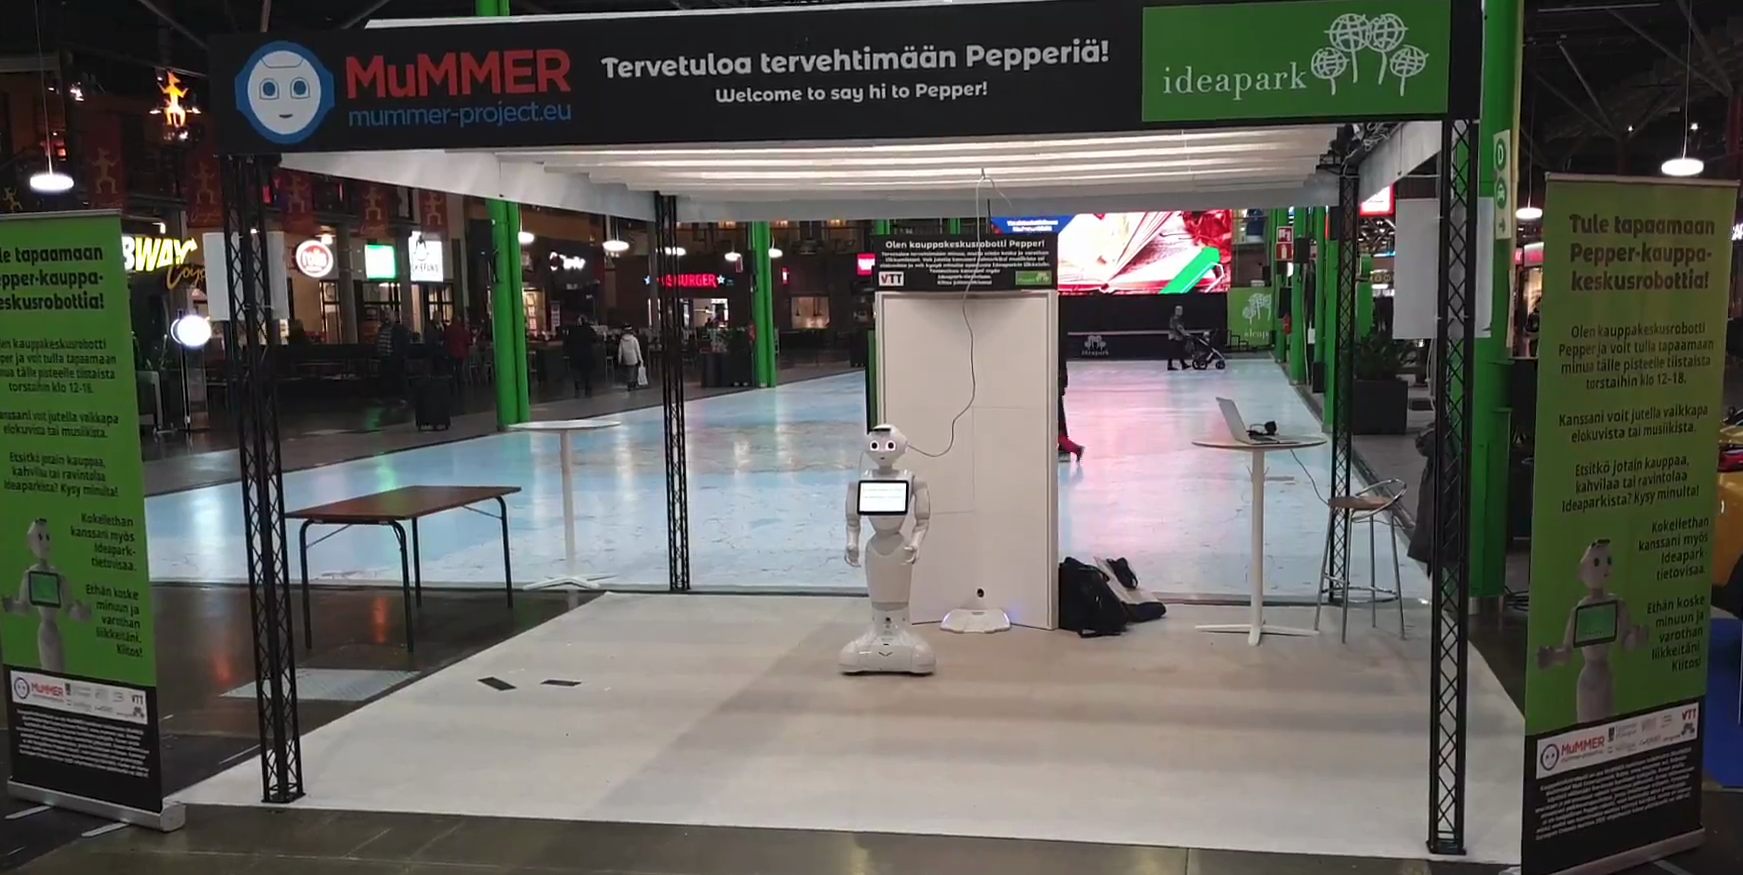
\includegraphics[scale=0.2]{figures/chapter3/pepper_mall.png}
	\caption{\label{fig:chap3_pepper_mall} The pepper robot in its interaction area in the Finalnd mall, Ideapark. }
\end{figure}

During the first deployment in the real mall, we have updated both the Geometric Representation with actual measurements and the \acrfull{ssr} by making sure the regions, interfaces, corridors and intersections were represented reflecting the actual mall topology. To ensure the correctness of the instructions given by the route handler, we generated routes from the deployment location to several shops in the mall and followed them to the destination. Inaccuracies, as well as algorithmic flaws, have been fixed using this method. We also tested the interaction in the Finnish language with our native Finnish partners and corrected some mistakes in the route verbalization.

\subsection{The deliberative architecture embedded in a physical robot}\label{subsec:archi-integration}

In the previous section, we presented a deliberative architecture designed to be embedded in a service robot. The purpose of this robot was to be deployed in a mall in Finland. 
To make this deployment successful, we did extensive tests in our laboratory where we had reproduced a part of the mall environment to be in the most realistic conditions possible\footnote{This setup not only was used for tests but also for public demos and even in the context of a scientific live event now accessible on \url{https://youtu.be/p4f3iwHht2Q?t=4495}}. Some of these emulated shop are visible in Fig.~\ref{fig:chap3_lab_shops}. 
In Sect.~\ref{subsec:setup_mall}, we introduce the environment setup as well as the robot one. Then, in Sect.~\ref{subsec:tests_mall} and Sect.~\ref{subsec:deploy}, we present our tests and deployment in the Finnish mall. 

\begin{figure}[!htp]
   \subfloat[A person being guided, the emulated shop ``Zizzi'' is visible in the background of the picture.]{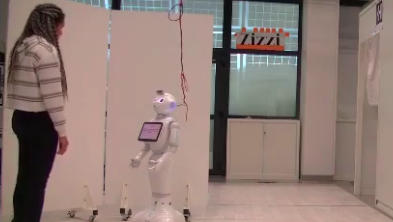
\includegraphics[width=0.49\linewidth]{figures/chapter3/lab1.png}}\hfill
   \subfloat[A person being guided, the emulated shop ``H\&M'' is visible.]{\includegraphics[width=0.49\linewidth]{figures/chapter3/lab4.png}}\hfill
   \subfloat[Two people simulated going to shop. The emulated shop ``Burger King'' is visible in the background and a small part of ``Thai Papaya'' is visible in the foreground.]{\includegraphics[width=0.49\linewidth]{figures/chapter3/lab3.jpg}}\hfill
   \subfloat[A person being guided, a sign towards the toilet and the shop ``Marco Polo'' are visible on the left of the picture.]{\includegraphics[width=0.49\linewidth]{figures/chapter3/lab2.png}}\hfill
   \caption{Examples of emulated shops of the Finnish mall in our lab.}
   \label{fig:chap3_lab_shops}
\end{figure}

\subsubsection{Environment and robot setup in the Finnish mall}\label{subsec:setup_mall}
Our architecture has been tested and deployed in a mall in Finland. As we explained previously, it has two abilities: chat with people and guide them, but in this paper we consider only the latter. The robot was able to interact in English and Finnish, though due to the vast linguistic differences between the two languages, the two versions have been kept separated, and the whole interaction can either be in one or the other. 


\paragraph{Hardware architecture}\label{subsec:hw}
The robot is an upgraded, custom version of the Pepper platform~\cite{caniot_adapted_2020}, which is equipped with an Intel D435 camera and an NVIDIA Jetson TX2 in addition to the traditional sensors that are found on the previous versions of the robot. We used the Robot Operating System (ROS) to enable inter-process communication between the processing nodes. All the streams (audio, video, robot states) are sent to a remote laptop which performs all the computation. The laptop has an NVIDIA RTX 2080 graphics card (for the visual perception system) and 12 CPU cores. The 4 microphone streams are processed at a frequency of $16000$~Hz, and the full perception system delivers the output at 10~fps.

\subsubsection{Pre-deployment in the Finnish mall, in-situ tests}\label{subsec:tests_mall}

Three integration sessions, each lasting one week have been made on site, in September 2018, June 2019 and September 2019, in the mall in Finland. The whole LAAS developer team were part of these integration weeks, along with our project partners. So, I spent around 150 hours (3 times 5 days) in the mall for software integration debugging with the other developers, and testing and debugging of the direction-giving task. 
During the integration weeks, only expert users (developers) interacted with the robot for testing purpose. 

To have a working system in the lab and to have a working system in a real-world site are two different things. As much as a team prepare for an in-situ deployment, there will always be elements that will need to be tuned on site and unexpected bugs arising. Thus, I had to handle a lot of contingencies, diagnosing where the issue came from, repairing if it was originating from my software, communicating with the person responsible for the component having a bug if it was not from mine, and testing again.

The first step to perform for us once on site was to update both the Geometric Representation (see Sect.~\ref{subsec:models}) which was previously based on architectural plans and refined with actual measurements and the \acrlong{ssr} (see Sect.~\ref{subsec:models}) by making sure the regions, interfaces, corridors and intersections were represented reflecting the actual mall topology. 

Finally, to ensure the correctness of the instructions given by the route handler, we generated routes from the deployment location to random shops in the mall, and followed them to the destination. \acrshort{ssr} inaccuracies as well as algorithmic flaws have been fixed using this method. We also tested the interaction in Finnish language with our native Finnish partners and corrected some mistakes in the route verbalization.


\paragraph{Component integration problematic}
Even though components were integrated together before getting on site, code modifications as mentioned above and intense testing can make new issues appear. So, it was essential to test the integration between all the components after this.

Finally, once everything was running quite nicely, some time has been dedicated to fine-tune the direction-giving task, ensuring all the components could withstand running for several hours in a row, with naive users possibly interrupting the task at any stage. 

\subsubsection{``In the wild'' deployment}\label{subsec:deploy}
\begin{figure}
	\centering
	\includegraphics[width=\linewidth]{figures/chapter3/guided_person.jpg}
	\caption{A person receiving directions from Pepper. (Image from VTT team)}
	\label{fig:guided_person}
\end{figure}
The robot was then installed for a long-term 14 weeks deployment from September 2019 to December 2019. During this period, the robot interacted with everyday clients of the mall, who may never had the chance to interact with a robot before. The robot was active for 3 hours per day, three days a week. As it was a project with multiple partners, it was not always possible to have our direction-giving task running. The direction giving task has been available on the robot 32 days out of the 42. The days during which it was not running, the partners' software executing on the robot where the visual perception and the dialogue that we mentioned previously, and a social signal processing feature~\cite{foster2019mummer}.

Nowadays, having an autonomous robot in the wild is a challenge. At first glance, we could think that if the robot is able to run smoothly for a few hours, the challenge would be met. However, there are a lot of other elements to take into account. First, how to guarantee the safety of children and elderly? How to ensure that the robot will not fell on or bump into them despite the robot sensors, hurting them? Furthermore, not only people safety is important but making sure that the robot is not damaged by people as well. People might indeed be brutal towards the robot, on purpose or not. 

To tackle the ``obvious'' issue, making sure that the robot continuously running, it was remotely watched by an on-call developer of the project team. At the beginning of the time slot, they launched all the software on the robot. Then, they checked through component monitoring, time to time, if everything was running properly, and they were in contact with the robot guard who told them if she noticed something wrong with the robot. They also had access to a video feed of the robot home-base if needed. Thus, all along this long-term deployment, we adjusted parameters and fixed bugs, with the help of the on-site team VTT and the robot guard that tested the direction-giving task when we asked her. The bugs we encountered concerned mainly Finnish translation issues (e.g. ``just after Arnold's'' was translated ``paikan päälle Arnolds'' in Finnish but the correct way to say it in Finnish was ``paikan Arnolds jälkeen'' thus we changed the English sentence into ``right after the place Arnolds'' to be able to get this translation), shop names issues (e.g. Finnish people use the utterance ``Hennes Mauritz'' and not ``H\&M'' which was the name in the robot ontology originally) and route issues (e.g. a route has one more turn than it should have).

The project consortium tackled the two safety issues (people safety and robot safety) by hiring a ``robot guard'' and by putting a sign notifying parents to not leave their children alone with the robot. During the robot active hours, this guard employee was physically present to ensure people were respectful towards the robot, \ie not hitting it or pulling it, to watch the kids who may get too close to the robot when it could have moved so they would not risk to be hurt, and to answer people who wanted to know more about the robot or the project than what was explained on the explanatory posters. She was also responsible for starting and shutting down the robot at the beginning and at the end of the half-day. Besides, for security and legal responsibility reasons, we chose to not have the robot navigating during this deployment as it would have been a complicated issue if the robot bumped into someone, especially a kid who could be hurt. It would have been possible if Pepper had a remote emergency stop which could have been given to the guard. Therefore, the step \textit{Ensuring correct placement} was removed in this context. Then, the Human-Aware Navigation component (see Sect.~\ref{subsec:navigation}) was disabled and the Shared Visual Perspective Planner (see Sect.~\ref{subsec:svp}) was only used to compute the 360 degrees visibility of a landmark from the person position.


In total, the robot ran the direction-giving task during approximately 96 hours ``in the wild''. Out of these 96 hours, it was interacting with someone during 45 hours. Table~\ref{tab:stats_sessions} summarizes statistical data about the interaction sessions and Table~\ref{tab:stats_tasks} summarizes statistical data about the direction-giving tasks.

\begin{table}[htp]
	\centering
	\begin{tabular}{p{0.8\linewidth}|p{0.1\linewidth}}
		\hline
		Description & Value \\ 
		\hline
		Number of occurred interaction sessions between a human and the robot &  979 \\ 
		Cumulative duration of the interaction sessions  & 2720 min \\ 
		Minimal duration of an interaction session  & 0.1 min \\ 
		Maximal duration of an interaction session & 41 min \\
		Average duration of an interaction session & 2.8 min \\
		Standard deviation of sessions duration & 3.3 min \\
		Average number of direction-giving tasks during a session & 1.1 \\
		Percentage of sessions terminated by goodbyes & 30\% \\
		Percentage of sessions terminated by the participant not perceived by the robot anymore & 70\% \\
		\hline
	\end{tabular}
	\caption{Statistics on interaction sessions in the wild}
	\label{tab:stats_sessions}
\end{table}


\begin{table}[htp]
	\centering
	\begin{tabular}{p{0.8\linewidth}|p{0.1\linewidth}}
		\hline
		Description & Value \\ 
		\hline
		Number of occurred direction-giving tasks between a human and the robot &  1156 \\ 
		Cumulative duration of the direction-giving tasks & 930 min\\ 
		Minimal duration of a direction-giving task & 0.01 min \\ 
		Maximal duration of a direction-giving task & 22 min \\
		Average duration of a direction-giving task & 0.8 min \\
		Standard deviation of direction-giving tasks duration & 1.27 min \\
		Success rate of the step \textit{Establishing the shared goal} & 63\% \\
		Success rate of the step \textit{Route planning according to the human willingness and ability to climb stairs} & 100\% \\
		Success rate of the step \textit{Pointing to target} & 56\% \\
		Success rate of the step \textit{Ensuring target seen} & 39\% \\
		Success rate of the step \textit{Pointing to passage and giving route directions} & 94 \% \\
		Success rate of the step \textit{Ensuring passage seen or route understood} & 92\% \\
		Success rate of the removed step \textit{Check if indications understood} & 19\% \\
		\hline
	\end{tabular}
	\caption{Statistics on the direction-giving task in the wild. \textit{Ensuring target seen} is a part of the step \textit{Pointing to target} as described in Sect.~\ref{sec:guiding}. Likewise,  \textit{Ensuring passage seen or route understood} is a part of the step \textit{Pointing to passage and giving route directions}. The success rate of a step is the number of times the given step has been achieved over the number of times it was planned (e.g. \textit{Route directions and pointing} is not planned if there is no passage to point), all direction-giving tasks combined. Steps were not achieved sometimes because of robot failures but most of the time it was because the human was leaving during the task. As mentioned in Section~\ref{par:route_understood}, we did not keep the step \textit{Check if indications understood} all along the deployment because, as shown by the success rate, people were leaving before answering this question. Then, as this step was considered as superfluous by users, we merged it with the one before, \textit{Ensuring passage seen}.}
	\label{tab:stats_tasks}
\end{table}


\section{Integration and test of the QoI Evaluator}\label{sec:qoi_integration}
As a proof-of-concept for the QoI Evaluator presented in Section~\ref{sec:qoi} of the Chapter~\ref{chapter:chap2}, we integrated it in the direction-giving task described in this chapter.


More specifically, this implementation of the Quality of Interaction Evaluator measured the interaction quality at the direction-giving task level and at the elementary actions level, omitting the interaction session level as this latter was not our focus in the \acrshort{mummer} project. The QoI Evaluator was integrated into \acrshort{jahrvis} presented in Chapter~\ref{chapter:chap2}. The QoI Evaluator is implemented into a Jason function (the reasoning cycle) which is invoked periodically. After multiple testings, we reached the conclusion that it was pertinent, at least in the context of the direction-giving task, to have the Evaluator computing the QoI every second for both levels. Therefore, every second, the system computes the value of each metric and then outputs a value for $QoI_{task}$ and $QoI_{action}$. 

\begin{figure}[!htp]
	\subfloat[A customer listening to Pepper after re-positioning]{\includegraphics[width=0.49\linewidth]{figures/chapter3/human_1_mall.png}}\hfill
	\subfloat[A customer listening and Pepper pointing to a corridor]{\includegraphics[width=0.49\linewidth]{figures/chapter3/human_2_mall.png}}\hfill
	\subfloat[A customer answering to Pepper]{\includegraphics[width=0.49\linewidth]{figures/chapter3/human_3_mall.png}}\hfill
	\subfloat[A customer listening and Pepper pointing to a shop]{\includegraphics[width=0.49\linewidth]{figures/chapter3/human_4_mall.png}}\hfill
	\caption{MuMMER robot engaged in direction-giving tasks. Around 350 trials with customers in the mall allowed us to gather empirical data to select the metrics and tune the measuring functions parameters.}
	\label{fig:customers}
\end{figure}

As mentioned in the step \ref{list:mall} of the chronicle, the robot interacted in the wild with dozens of usual customers (Fig.~\ref{fig:customers}), executing around 350 direction-giving tasks. This allowed us to improve the performance of the direction-giving task, to gather standard durations of the subtasks executions and to draw lessons about metric definitions and choices (e.g. we realized it was not relevant to measure the human visual attention towards the robot when it was giving the route explanation as humans look around at this moment). Unfortunately, the practical conditions of the project deployments did not offer us the possibility to evaluate the QoI Evaluator based on a study in the mall with real customers. So, we demonstrated -- after improvements of the metrics equations such as the Distance-to-Goal one, and manual tuning of their parameters based on the experience in the mall -- our finalized concept through tests in our lab (step~\ref{list:refin}). This is shown in Sect.~\ref{subsec:results} where we present and discuss, a comparison of the QoI computed by the robot when it is dealing with an ``ideal'' human, a ``confused'' human and a ``non-compliant'' human during a direction-giving task, performed in the lab. Before that, we present in Sect.~\ref{subsec:task_qoi} and Sect.~\ref{subsec:action_qoi} how the QoI is evaluated at both task and action levels for the direction-giving task.

\subsection{QoI Evaluation at the task level}\label{subsec:task_qoi}

In the context of the direction-giving task, we have selected two metrics to evaluate the QoI at the task level: a metric defined in the Sect.~\ref{sec:metrics}, the \textit{Deviation from standard duration} and, the aggregation over time of the actions QoIs. Following the process of Fig.~\ref{fig:qoi_schema}, we measure the QoI of the $\text{Task}_i = \text{direction-giving\_task}$, based on the QoI of all task actions and $\text{Task metric}_1$ = Deviation from standard duration.

The \textit{Deviation from standard duration} is used to measure the QoI at the task level as the task is a sequence of subtasks. Indeed, if the subtask lasts longer than expected, the QoI should decrease. Then, as needed for the metric computation we have determined the values of the soft deadlines $SD_i$ for each subtask $a_i, i \in [0,4] $, using the empirical data we gathered as explained in\todo{ref sec}. Specifically, we have computed the average time execution of each subtask, after removing the cases for which the execution of the subtask was annotated as not smooth. These soft deadlines are presented in table~\ref{tab:dl}. Finally, we chose $V_i=0.5$ for all the subtasks.
\begin{table}[ht]
	\centering
	\begin{tabular}{l|c}
		\hline
		Subtasks & soft deadline (s) \\ 
		\hline
		Target refinement process &  30 \\ 
		Ensuring Correct HR Placement   & 30 \\ 
		Ensuring target seen  & 20 \\ 
		Direction explanation and pointing & 30 \\
		Ensuring Direction Seen & 20\\
		\hline
	\end{tabular}
	\caption{Soft deadlines $SD_i$ for each subtask of the direction-giving task}
	\label{tab:dl}
\end{table}

The task QoI is also dependent on the actions QoI values (their computation is described in Sect.~\ref{subsec:action_qoi}). Indeed, the actions QoIs should be reflected on the task QoI as, if a majority of the actions have a low QoI, the task QoI cannot remain high. That is why, besides the\textit{ Deviation from standard duration}, we take into account the average of the action QoIs of the actions already executed or still running.

Then, the task QoI is computed using Equation~\eqref{eq:qoi} presented in Sect.~\ref{sec:eval}. After various trials we have empirically chosen the weights $W_i$ for each metric $M_i, i \in [0,1]$. The final equation to compute the task QoI is:
\[QoI_{dir-giv\_task}(t)=\frac{ \Phi_{dir-giv\_task}(t) + 3 * \overline{QoI}_{actions} }{4}\]

\subsection{QoI Evaluation at the action level}\label{subsec:action_qoi}
As mentioned earlier, each subtask of the direction-giving task can be decomposed into actions. These actions involve several turn-taking steps, the robot asking complementary information, informing the human or expecting an action or reaction from them. We need to measure the QoI during the execution of each action. To do so, we have chosen one or more metrics for each action. 

\setlength\tabcolsep{1.5pt}
\begin{table*}[ht]
	\centering
	\begin{tabular}{|c|p{1.5cm}|c|c|}
		Metric id & Metric name & Metric equation -- with Equations of Section~\ref{sec:metrics} & Scaled metric -- with functions of Appendix~\ref{annex:functions} \\\hline\hline
		
		\(\displaystyle M_{H\_contrib}\)
		& Human contribution to the goal 
		& \raisebox{-0.5cm}{ \(\displaystyle nb\_R\_repet \)} &  \raisebox{-0.5cm}{ \(\displaystyle n_1(nb\_R\_repet) = 2 * \dfrac{nb\_R\_repet-3}{-3} -1 \)} \\\hline
		
		\(\displaystyle M_{Exp\_SI}\)
		& Fulfilling robot expectations about social interaction 
		&    \raisebox{-0.5cm}{ \(\displaystyle Ar = \frac{duration_{isAttentiveTo(robot)=true}}{duration_{robot\_speaks}} \) }
		&  \raisebox{-0.5cm}{\(\displaystyle n_1(Ar) = 2 * Ar -1 \)} \\\hline
		
		\(\displaystyle M_{DtG}\)
		& Distance-to-Goal & 
		\(\displaystyle \left\{
		\begin{array}{ll}
		\Delta DtG(t=0) = 0\\
		\begin{aligned}
		\Delta& DtG(t) = \max(0,\Delta DtG(t-1) - 1)  \\&\text{if } path\_length(t) <  path\_length(t-1) \\
		
		\end{aligned}\\
		\Delta DtG(t)= \Delta DtG(t-1) + 1, \text{otherwise.}
		
		\end{array}
		\right.
		\)
		&   \(\displaystyle -s_1(DtG(t)) = -1 + 2 \exp{\left(-\ln{(2)}\left(\dfrac{DtG(t)}{5}\right)^{1.5}\right)} \) \\\hline
		
		\(\displaystyle M_{TtG}\)
		& Time-To-Goal & 
		\(\displaystyle \Delta TtG(t) = \max(0, e(t)  + TtG(t) - TtG(T_0)) 
		\)
		&  \(\displaystyle -s_1(TtG(t)) = -1 + 2 \exp{\left(-\ln{(2)}\left(\dfrac{TtG(t)}{5}\right)^{1.5}\right)} \) \\
		
		
	\end{tabular}
	\caption{Metrics used in the implementation presented in Section~\ref{sec:qoi_integration}.}
	\label{tab:metrics_impl}
\end{table*}  


For each action of the following list, we explain which metrics $M$ of Table~\ref{tab:metrics_impl} we have used and scaling functions of Appendix~\ref{annex:functions} and then, how we compute the action QoI. 
\begin{enumerate}[label=(\alph*)]
	\item \label{list_act:info} \textit{Robot-Human information sharing: }The robot speaks to the human, shares information such as the route direction and announces the next steps of the plan. The robot expects that they are paying attention to it. Therefore, we use the \textit{Fulfilling robot expectations about social interaction} $M_{Exp\_SI}$ based on the attention ratio. Two parameters need to be defined for the scaling function, the bounds $b_1$ and $b_2$. As the minimum value for the metric, a ratio, is 0 and the maximum value is 1, then $b_1=0$ and $b_2=1$. 
	The QoI of the action is computed with this only metric.
	
	\item \label{list_act:qa} \textit{Human-Robot Q/A process: } The robot asks a question to the human. As for the previous action, the robot expects the human to pay attention to it so we compute the QoI with $M_{Exp\_SI}$. It also expects the human to give an appropriate answer. If it does not happen, it will ask the human to repeat, specifying that the answer has not been understood. We have limited the possible number of attempts to 3. After 3 attempts, the robot ends the task, as it cannot carry on with the task without an answer. So, we use \textit{Human contribution to the goal} $M_{H\_contrib}$, the number of times the robot repeats. Because the maximal number of repetitions is 3, we set for the scaling function $b_1=3$ and $b_2=0$.
	
	The QoI is computed with the two metrics: \textit{Fulfilling robot expectations about social interaction} and \textit{Human contribution to the goal}.
	The trials showed that the action QoI results were satisfying with the weights $W_i=1, i \in [0,1]$ as applying the Equation~\eqref{eq:qoi}.
	
	\item \label{list_act:moves_aside} \textit{Ensuring that Human  moves aside: }This action is used if, for pointing, the robot decides to place itself in a position which is very close to where the human is currently standing. In this case, the robot asks the human to step aside to the right or left, depending on the human's future position. Then, we want to measure the progress of the human going further from the planned robot position. In order to do this, we use the \textit{Distance-to-Goal} $M_{DtG}$ but with the condition of the $\Delta DtG$ equation adapted, being $\text{if } path\_length(t) >  path\_length(t-1)$ instead of $\text{if } path\_length(t) <  path\_length(t-1)$. We scale the metric with  $-s_1$, the additive inverse of the scaling function and not directly $s_1$ as the closer to 0 $\Delta DtG$ is, the better it is in terms of goal completion. From trials, we set $-s_1$ parameters values with $th=5$ and $k=1.5$.
	
	If the human does not move or does not go far enough from the robot position, the robot will ask again with a limit of 3 trials (if the robot cannot move, it will carry on the task from their current positions). So, we use $M_{H\_contrib}$ as for the previous action. 
	
	\item \label{list_act:nav} \textit{Human-aware robot navigation: }The robot has to move from its initial position to its computed one. It navigates while respecting social constraints and its path may change as it adapts according to what the human is doing. At execution time, to measure the robot progress towards its goal, we use the \textit{Time-to-goal} $M_{TtG}$, with the same scaling function than $M_{DtG}$. The QoI of the action is computed with this only metric. 
	
	\item \label{list_act:correct_place1} \textit{Ensuring correct human placement for verbal interaction: }After it has moved, the robot asks the human to come in front of it. If the human is not perceived after a few seconds, the robot will ask again and so on in a maximum of 3 trials. If after these 3 times the human is still not perceived, the robot ends the task. 
	
	The QoI of this action is computed with $M_{H\_contrib}$ -- we do not use $M_{Exp\_SI}$ as the human is not in the field of view when the robot is calling them.
	
	\item \label{list_act:correct_place2} \textit{Ensuring correct human placement for route explanation: }Once the human is in the robot field of view after the HR motion, they may not be at the right place to properly see what the robot has to point at. In this case, the robot will ask the human to move forward or backward according to what it has computed about the human perspective (e.g. this is to avoid that an object occludes the view for the human). Then, we want to measure the human progress towards the position the robot has computed for them. In order to do this, we use the \textit{Distance-to-Goal} $M_{DtG}$.
	
	The robot stops giving instructions if it computes that the position of the human allows them to see the target, or after 3 trials, so we use $M_{H\_contrib}$. After 3 trials, if the human cannot see the target, still, the robot will carry on the task taking this into account.
	
	
\end{enumerate}

\begin{table}[!h]
	\begin{center}
		\begin{tabular}{ | c || c | c | }
			\hline
			Mall elements                   & Mockup mall & Real mall \\ \hline \hline
			Shops              & 19            & 140   \\ \hline
			Doors, stairs, elevators & 10            & 50    \\ \hline
			Corridors              & 11            & 41    \\ \hline
			Levels   & 2            & 2   \\ 
			\hline
		\end{tabular}
	\end{center}
	\caption{\label{tab:malls} Number of elements described in the mockup and real malls (geometric, topologic and semantic models in Fig.~\ref{fig:chap3_3Dmodels}).}
\end{table}

\bgroup
\def\arraystretch{2.5}
\begin{table}[t]
	\centering
	\begin{tabular}{|p{3.5cm}|c|}
		Action & QoI formula (metric aggregation) \\ \hline \hline
		Robot-Human information sharing & $ M_{Exp\_SI}(t)$ \\ \hline
		Human-Robot Q/A process & \(\displaystyle\frac{M_{Exp\_SI}(t) + M_{H\_contrib}(t) }{2}\) \\ \hline
		Ensuring  that  Human  moves  aside  & \(\displaystyle\frac{M_{DtG}(t) + M_{H\_contrib}(t) }{2}\) \\ \hline
		Human-aware robot navigation  & $M_{TtG}(t)$ \\ \hline
		Ensuring correct human placement for verbal interaction & $M_{H\_contrib}(t)$ \\ \hline
		Ensuring correct human placement for route explanation & \(\displaystyle\frac{M_{DtG}(t) + M_{H\_contrib}(t) }{2}\) 
	\end{tabular}
	\caption{QoI computation for each action as an aggregation of metrics}
	\label{tab:qoi}
\end{table}
\egroup

\begin{figure*}[!ht]
	\centering
	\subfloat[Evolution over time of the measured QoI for the 'ideal' human. Both action and task QoIs remain at 1 as the task is proceeding smoothly. ]{\label{fig:human_ideal}\includegraphics [width=\linewidth]{figures/chapter3/human_ideal.png}}\hfill
	\subfloat[Evolution over time of the measured QoI for the ``confused'' human. They took time to answer the first robot question and to move forward but the task QoI does not drop too much because the robot was able to give the route explanation without any issue even though the human was not very attentive. ]{\label{fig:human_confused}\includegraphics[width=\linewidth]{figures/chapter3/human_confused.png}}\hfill 
	\subfloat[Evolution over time of the measured QoI for the non-compliant human. Several times the human did not give the expected answer to the robot during the target refinement process. Then, they blocked the robot path. After that, the robot had to ask twice the human to come in front of it. Finally, the robot repeated the route direction three times but still the human kept saying that they did not understand. Therefore, the task QoI decreases all along the task.] 
	{\label{fig:human_not_comp}\includegraphics[width=\linewidth]{figures/chapter3/human_not_comp.png}}\hfill
	\caption{Evolution over time of the measured QoI for the route guidance task with three different human behaviors. The QoI for the task is drawn in blue, and the QoI for the actions is drawn in orange.}
	\label{fig:impl_qoi}
\end{figure*}

\subsection{Proof-of-Concept}\label{subsec:results}
This section reports on an effective implementation of the approach as an illustrative proof of concept. We show the ability of the robot to conduct an interactive task, to assess in real-time the QoI and to track its evolution during three direction-giving task executions where the same human displayed a different way of behaving. In the three cases, the task was conducted until its end, in our lab where we reproduces the mall environment (Fig.~\ref{fig:chap3_lab}, Table~\ref{tab:malls}). The computed QoI for each way is presented in Fig.~\ref{fig:impl_qoi}. The three different ways of behaving are described in the following list:
\begin{itemize}
	\item A human executed perfectly the expected actions and was not disturbing the robot when it navigated (\ie the ``ideal'' human from the robot point of view). 
	\item A bit ``confused'' human tried to contribute to the task success but did not execute everything well. The human was, from time to time, not very attentive, as looking around. Also, they gave an answer to the first question that the robot did not understand, and then they took their time before answering again. Then, they prevented a bit the robot to move as it had planned and once the robot reached its position, they took time to come as close as the robot wanted. 
	\item A human wanted to disturb the robot during the task. They gave three incomprehensible answers to the first question, blocked multiple times the robot in its move, waited for the robot to ask twice to come in front of it and finally asked the robot to point and explain the route three times. 
\end{itemize}

Now, if we take a look at the QoI outputs of Fig.~\ref{fig:impl_qoi}, we can see that their three shapes are very different. In Fig.~\ref{fig:human_ideal}, we can observe that the task and actions QoIs remain with the highest value 1 all along. A graph as this one allows us to infer that everything went very smoothly during this direction-giving task. Then, we can guess that it corresponds to the execution performed with the 'ideal' human. 

In Fig.~\ref{fig:human_confused}, we note that each subtask was executed in respect of the standard duration. If the QoI of \textit{Target refinement process} drops it is because of the action QoI as the QoI of the \textit{H-R Q/A process} drops because the robot had to repeat the question and the human was not looking at it. From 21 seconds to 40 seconds, we can see the task QoI getting higher as the QoIs of \textit{Human-aware robot navigation}, \textit{Ensuring correct human placement for verbal interaction} and the beginning of \textit{Ensuring correct human placement for route explanation} are quite high. Next, seeing the shape of the computed QoI of the action \textit{Ensuring human placement for route explanation}, we can infer that the human was not moving as the robot wanted. Indeed, they took 10 seconds to make one step forward (they had 1 meter to cross). Because of that, the task QoI started to decrease again. In the final part of the task, the human was time to time attentive to the robot answered quickly to the last question, so the task QoI remained rather equal with its final value being $0.34$ which is above 0 so meaning a correct interaction.

\begin{figure}[!t]
	\centering
	\begin{subfloat}[Human who put themselves on the robot path, preventing the robot to navigate towards its goal position]{
			\includegraphics[width=0.29\linewidth]{figures/chapter3/blocking1.png}}\hfill
	\end{subfloat}
	\begin{subfloat}[Human who put themselves on the robot path after it computed a new path to reach its goal position]{
			\includegraphics[width=0.29\linewidth]{figures/chapter3/blocking2.png}}\hfill
	\end{subfloat}
	\begin{subfloat}[Human finally getting outside of the robot path, allowing it to reach its goal position]{
			\includegraphics[width=0.29\linewidth]{figures/chapter3/not_blocking.png}}\hfill
	\end{subfloat}
	\caption{A human disturbing the robot during \textit{Human-aware navigation}, preventing it to reach its goal position as planned.}
	\label{fig:blockig_nav}
\end{figure}

Finally, we can see in Fig.~\ref{fig:human_not_comp} that the final QoI of the task is $-0.44$ which allows us to infer that the task was not executed smoothly. And indeed, when we look at the shape of the task QoI, it only went down (or almost) all along the task. It is explained by some subtasks that took more time than they should have and also by some actions QoIs that are very low, especially the one of \textit{Human-aware robot navigation}. At the beginning of the robot navigation, the estimated time to goal returned by the planner was 6 seconds but the robot actually took 50 seconds to reach its goal then the action QoI computed with $=M_{TtG}(t)$ was $-1$ for $40$ seconds. And indeed, all along its navigation, the human was blocking the robot until they got tired of this game, as visible on Fig.~\ref{fig:blockig_nav}.

In this example, we showed the QoI evaluation process integrated to a complete robotic architecture. The robot was able to assess the QoI in real-time while interacting with a human.

\subsection{Discussion on the results of the QoI Evaluator}
While a number of evaluation methods has been proposed to evaluate a human-robot interaction from the human perspective and often for analysis after performance, our choice to let the robot evaluate, on its own and in real-time the quality of its interaction with a human is quite new and original. To endow the robot with such an ability, we designed, implemented and tested a number of metrics and a method to aggregate them.

The work of Steinfeld \textit{et al}.~\cite{steinfeld_2006_common} was very helpful to design a first set of metrics and as an inspiration about what could be used. From there, we have elaborated and proposed a set of metrics which are meant to estimate of the quality of an ongoing interaction and not once it is over. 
The work of Hoffman~\cite{hoffman2019} regarding the \textit{fluency} definition and how to measure it was also inspiring. In a way, we extended his work by giving a meaning to the fluency measurement on the robot side, and in real-time -- while their work applies to offline evaluation of shared workspace tasks. 
In Sect.~\ref{sec:rel}, we mentioned systems measuring human affective states in real-time such as the framework developed by Tanevaska \textit{et al}~\cite{tanevska:hal-01615491}. Although we think such metric could be an interesting additional information to assess if an interaction is going well, we believe that these measurements do not offer an accuracy that would lead to objective measurement of the quality of interaction, thus, we did not introduce them in our set for now. However, this could be done since our framework is designed to be open to new metrics. 
As for contributions, like the one proposed by Anzalone \textit{et al}.~\cite{anzalone_2015_evaluating}, based on metrics such as gaze, head pose, body pose and response times to measure real-time engagement, we took them into account to some extent. However, the measure of the engagement that we propose should be refined depending on the inputs available on-line to the robot . Moreover, we will investigate how their work could be used in a more general way (e.g. depending on the action that should be done and its context, human head pose and body posture could be a good indicator of effectiveness and not only engagement). 

Our intention, when we developed the idea of the Quality of Interaction Evaluation, was to use such computation to feed the decision-making process of the robot and this is what we intend to do in the future. However, such framework can also be used to compare interactions between different humans and/or robots, eventually as a benchmark similarly to the work of Sanchez-Matilla~\cite{sanchez} or as a way for developers to detect repetitive interaction issues with an unsupervised robot in a real-world environment.

As a proof-of-concept, we implemented and deployed a first version of a QoI Evaluator assessing task and actions QoIs. We tested it on an interactive robot dedicated to provide route guidance to customers in a large mall. The approach gave satisfactory results. It showed the potential ability of a robot to detect momentary decreases of the Quality of Interaction and also more serious degradation of it which may need drastic change of behavior for the robot. This is only a first step and it should be validated with a study where we will ask humans to evaluate the quality of their interaction with the robot in a similar manner. The goal will be to analyse and compare this to the evaluation of the interaction quality estimated by our robot and, based on that, investigate potential improvements. 

Finally, we do not claim to have a perfect measure of the Quality of Interaction. However, although the concept of Quality of Interaction is quite abstract, Movellan \textit{et al.} showed that when it is measured by human observers, the inter-observer reliability of the concept is quite high. Therefore, we believe we can endow the robot with an effective and pertinent ability aiming at measuring the quality of an interaction. We are aware that the set of metrics we proposed to do so is not exhaustive but the framework is designed to be easily extended with new metrics.

\section{User Study}

\ifdefined\included
\else
\bibliographystyle{acm}
\bibliography{These}
\end{document}
\fi

\ifdefined\included
\else
\documentclass[a4paper,11pt,twoside]{StyleThese}
\usepackage{amsmath,amssymb, amsthm}             % AMS Math
\usepackage[T1]{fontenc}
\usepackage[utf8x]{inputenc}
\usepackage{babel}
\usepackage{datetime}

\usepackage{silence}

\WarningFilter{minitoc(hints)}{W0023}
\WarningFilter{minitoc(hints)}{W0028}
\WarningFilter{minitoc(hints)}{W0030}

\usepackage{lmodern}
\usepackage{tabularx}
%\usepackage{tabular}
\usepackage{multirow}
\usepackage{xspace}

\usepackage{subfig}
\usepackage[inline]{enumitem}

\usepackage{hhline}
\usepackage[left=1.5in,right=1.3in,top=1.1in,bottom=1.1in,includefoot,includehead,headheight=13.6pt]{geometry}
\renewcommand{\baselinestretch}{1.05}

% Table of contents for each chapter

\usepackage[nottoc, notlof, notlot]{tocbibind}
\usepackage{minitoc}
\setcounter{minitocdepth}{2}
\mtcindent=15pt
% Use \minitoc where to put a table of contents

\usepackage{aecompl}

% Glossary / list of abbreviations

\usepackage[intoc]{nomencl}
\iftoggle{ThesisInEnglish}{%
\renewcommand{\nomname}{Glossary}
}{ %
\renewcommand{\nomname}{Liste des Abréviations}
}

\usepackage{etoolbox}
\renewcommand\nomgroup[1]{%
  \item[\bfseries
  \ifstrequal{#1}{A}{Number Sets}{%
  \ifstrequal{#1}{G}{Agents Beliefs and Action Models}{%
  \ifstrequal{#1}{N}{Navigation}{%
  \ifstrequal{#1}{O}{Ontology}{%
  \ifstrequal{#1}{R}{Referring Expression Generation}{%
  \ifstrequal{#1}{Z}{Controllable and Uncontrollable Agents Task Planning}{}}}}}}%
]}

\makenomenclature



% My pdf code

\usepackage{ifpdf}

\ifpdf
  \usepackage[pdftex]{graphicx}
  \DeclareGraphicsExtensions{.jpg}
  \usepackage[pagebackref,hyperindex=true]{hyperref}
  \usepackage{tikz}
  \usetikzlibrary{arrows,shapes,calc}
\else
  \usepackage{graphicx}
  \DeclareGraphicsExtensions{.ps,.eps}
  \usepackage[dvipdfm,pagebackref,hyperindex=true]{hyperref}
\fi

\graphicspath{{.}{images/}}

%% nicer backref links. NOTE: The flag ThesisInEnglish is used to define the
% language in the back references. Read more about it in These.tex

\iftoggle{ThesisInEnglish}{%
\renewcommand*{\backref}[1]{}
\renewcommand*{\backrefalt}[4]{%
\ifcase #1 %
(Not cited.)%
\or
(Cited in page~#2.)%
\else
(Cited in pages~#2.)%
\fi}
\renewcommand*{\backrefsep}{, }
\renewcommand*{\backreftwosep}{ and~}
\renewcommand*{\backreflastsep}{ and~}
}{%
\renewcommand*{\backref}[1]{}
\renewcommand*{\backrefalt}[4]{%
\ifcase #1 %
(Non cité.)%
\or
(Cité en page~#2.)%
\else
(Cité en pages~#2.)%
\fi}
\renewcommand*{\backrefsep}{, }
\renewcommand*{\backreftwosep}{ et~}
\renewcommand*{\backreflastsep}{ et~}
}

% Links in pdf
\usepackage{color}
\definecolor{linkcol}{rgb}{0,0,0.4} 
\definecolor{citecol}{rgb}{0.5,0,0} 
\definecolor{linkcol}{rgb}{0,0,0} 
\definecolor{citecol}{rgb}{0,0,0}
% Change this to change the informations included in the pdf file

\hypersetup
{
bookmarksopen=true,
pdftitle="Endowing the robot with the abilities to control and evaluate its contribution to a human-robot joint action",
pdfauthor="Amandine MAYIMA", %auteur du document
pdfsubject="Thèse", %sujet du document
%pdftoolbar=false, %barre d'outils non visible
pdfmenubar=true, %barre de menu visible
pdfhighlight=/O, %effet d'un clic sur un lien hypertexte
colorlinks=true, %couleurs sur les liens hypertextes
pdfpagemode=None, %aucun mode de page
pdfpagelayout=SinglePage, %ouverture en simple page
pdffitwindow=true, %pages ouvertes entierement dans toute la fenetre
linkcolor=linkcol, %couleur des liens hypertextes internes
citecolor=citecol, %couleur des liens pour les citations
urlcolor=linkcol %couleur des liens pour les url
}

% definitions.
% -------------------

\setcounter{secnumdepth}{3}
\setcounter{tocdepth}{2}

% Some useful commands and shortcut for maths:  partial derivative and stuff

\newcommand{\pd}[2]{\frac{\partial #1}{\partial #2}}
\def\abs{\operatorname{abs}}
\def\argmax{\operatornamewithlimits{arg\,max}}
\def\argmin{\operatornamewithlimits{arg\,min}}
\def\diag{\operatorname{Diag}}
\newcommand{\eqRef}[1]{(\ref{#1})}

\usepackage{rotating}                    % Sideways of figures & tables
%\usepackage{bibunits}
%\usepackage[sectionbib]{chapterbib}          % Cross-reference package (Natural BiB)
%\usepackage{natbib}                  % Put References at the end of each chapter
                                         % Do not put 'sectionbib' option here.
                                         % Sectionbib option in 'natbib' will do.
\usepackage{fancyhdr}                    % Fancy Header and Footer

% \usepackage{txfonts}                     % Public Times New Roman text & math font
  
%%% Fancy Header %%%%%%%%%%%%%%%%%%%%%%%%%%%%%%%%%%%%%%%%%%%%%%%%%%%%%%%%%%%%%%%%%%
% Fancy Header Style Options

\pagestyle{fancy}                       % Sets fancy header and footer
\fancyfoot{}                            % Delete current footer settings

%\renewcommand{\chaptermark}[1]{         % Lower Case Chapter marker style
%  \markboth{\chaptername\ \thechapter.\ #1}}{}} %

%\renewcommand{\sectionmark}[1]{         % Lower case Section marker style
%  \markright{\thesection.\ #1}}         %

\fancyhead[LE,RO]{\bfseries\thepage}    % Page number (boldface) in left on even
% pages and right on odd pages
\fancyhead[RE]{\bfseries\nouppercase{\leftmark}}      % Chapter in the right on even pages
\fancyhead[LO]{\bfseries\nouppercase{\rightmark}}     % Section in the left on odd pages

\let\headruleORIG\headrule
\renewcommand{\headrule}{\color{black} \headruleORIG}
\renewcommand{\headrulewidth}{1.0pt}
\usepackage{colortbl}
\arrayrulecolor{black}

\fancypagestyle{plain}{
  \fancyhead{}
  \fancyfoot{}
  \renewcommand{\headrulewidth}{0pt}
}

%\usepackage{MyAlgorithm}
%\usepackage[noend]{MyAlgorithmic}
\usepackage{algorithm}
\usepackage[noend]{algpseudocode}
\usepackage{comment}
\usepackage[ED=MITT-InfoTel, Ets=INSA]{tlsflyleaf}
%%% Clear Header %%%%%%%%%%%%%%%%%%%%%%%%%%%%%%%%%%%%%%%%%%%%%%%%%%%%%%%%%%%%%%%%%%
% Clear Header Style on the Last Empty Odd pages
\makeatletter

\def\cleardoublepage{\clearpage\if@twoside \ifodd\c@page\else%
  \hbox{}%
  \thispagestyle{empty}%              % Empty header styles
  \newpage%
  \if@twocolumn\hbox{}\newpage\fi\fi\fi}

\newcommand*{\algrule}[1][\algorithmicindent]{%
	\makebox[#1][l]{%
		\hspace*{.2em}% <------------- This is where the rule starts from
		\vrule height .75\baselineskip depth .25\baselineskip
	}
}

%%% to have lines in algorithm, from stackexchange
\newcount\ALG@printindent@tempcnta
\def\ALG@printindent{%
	\ifnum \theALG@nested>0% is there anything to print
	\ifx\ALG@text\ALG@x@notext% is this an end group without any text?
	% do nothing
	\else
	\unskip
	% draw a rule for each indent level
	\ALG@printindent@tempcnta=1
	\loop
	\algrule[\csname ALG@ind@\the\ALG@printindent@tempcnta\endcsname]%
	\advance \ALG@printindent@tempcnta 1
	\ifnum \ALG@printindent@tempcnta<\numexpr\theALG@nested+1\relax
	\repeat
	\fi
	\fi
}
% the following line injects our new indent handling code in place of the default spacing
\patchcmd{\ALG@doentity}{\noindent\hskip\ALG@tlm}{\ALG@printindent}{}{\errmessage{failed to patch}}
\patchcmd{\ALG@doentity}{\item[]\nointerlineskip}{}{}{} % no spurious vertical space
% end vertical rule patch for algorithmicx

\makeatother
 
%%%%%%%%%%%%%%%%%%%%%%%%%%%%%%%%%%%%%%%%%%%%%%%%%%%%%%%%%%%%%%%%%%%%%%%%%%%%%%% 
% Prints your review date and 'Draft Version' (From Josullvn, CS, CMU)
\newcommand{\reviewtimetoday}[2]{\special{!userdict begin
    /bop-hook{gsave 20 710 translate 45 rotate 0.8 setgray
      /Times-Roman findfont 12 scalefont setfont 0 0   moveto (#1) show
      0 -12 moveto (#2) show grestore}def end}}
% You can turn on or off this option.
% \reviewtimetoday{\today}{Draft Version}
%%%%%%%%%%%%%%%%%%%%%%%%%%%%%%%%%%%%%%%%%%%%%%%%%%%%%%%%%%%%%%%%%%%%%%%%%%%%%%% 

\newenvironment{maxime}[1]
{
\vspace*{0cm}
\hfill
\begin{minipage}{0.5\textwidth}%
%\rule[0.5ex]{\textwidth}{0.1mm}\\%
\hrulefill $\:$ {\bf #1}\\
%\vspace*{-0.25cm}
\it 
}%
{%

\hrulefill
\vspace*{0.5cm}%
\end{minipage}
}

\let\minitocORIG\minitoc
\renewcommand{\minitoc}{\minitocORIG \vspace{1.5em}}

\usepackage{multirow}
%\usepackage{slashbox}

\newenvironment{bulletList}%
{ \begin{list}%
	{\tiny$\bullet$}%
	{\setlength{\labelwidth}{25pt}%
	 \setlength{\leftmargin}{30pt}%
	 \setlength{\itemsep}{-0.5em}}}%
{ \end{list} }

\newenvironment{inlineEnumerate}
{\begin{enumerate*} [label={(\arabic*)}] }
{\end{enumerate*}}

\theoremstyle{definition}
\newtheorem{definition}{Definition}
\renewcommand{\epsilon}{\varepsilon}

% centered page environment

\newenvironment{vcenterpage}
{\newpage\vspace*{\fill}\thispagestyle{empty}\renewcommand{\headrulewidth}{0pt}}
{\vspace*{\fill}}

\newenvironment{asl}{\ttfamily\begin{tabbing}~~~\=$\leftarrow$ \= ~~~ \=
		\kill}{\end{tabbing}}

\usepackage{tablefootnote}

\theoremstyle{plain}
\newtheorem{constraint}{Constraint}[section]

\algnewcommand\algorithmicforeach{\textbf{for each}}
\algnewcommand\algorithmicin{\textbf{in}}
\algdef{S}[FOR]{ForEach}[2]{\algorithmicforeach\ #1\ \algorithmicin\ #2\ \algorithmicdo}

\algnewcommand\algorithmicforkxor{\textbf{do fork-join-xor}}
\algnewcommand\algorithmicendforkxor{\textbf{end fork-join-xor}}
\algdef{SE}{ForkXor}{EndForkXor}{\algorithmicforkxor}{\algorithmicendforkxor}


\usepackage{listings}
\lstset{
	frame=single,
	captionpos=b,
	breaklines=true,
	basicstyle=\ttfamily,
	numberstyle=\color{black},
	tabsize=2,
	mathescape=true,
	literate=%
		{â}{{\^a}}1
}

\lstdefinestyle{inline}{
	frame=none,
	aboveskip=\smallskipamount,
	belowskip=\smallskipamount,
}

\lstdefinestyle{OwlTurtle}{
	language=C,
	tabsize=4,
	basicstyle=\scriptsize\ttfamily,
	keywordstyle=\bfseries\color{darkgray},
	morekeywords={rdf:type, rdfs:domain, rdfs:subPropertyOf, rdfs:range, :hasSubtask, :DecompositionUsedBy, rdfs:subClassOf, :hasDecomposition, owl:inverseOf, htn_actions:hasEffect, rdfs:label},
	alsoletter=:
}

\lstdefinestyle{aslDef}{
	frame=none,
%	breaklines=false,
	%xleftmargin=.1\textwidth, xrightmargin=.1\textwidth
}

\fancypagestyle{example}{%
	\fancyhead[LE]{\bfseries\thepage\includegraphics[scale=0.20]{figures/chapter2/task_goal.pdf}\includegraphics[scale=0.18]{figures/chapter2/task_setup_mini.pdf}}   
	\fancyhead[RO]{\includegraphics[scale=0.20]{figures/chapter2/task_goal.pdf}\includegraphics[scale=0.18]{figures/chapter2/task_setup_mini.pdf}\bfseries\thepage}  
	\fancyhead[RE]{\bfseries\nouppercase{\leftmark}}      % Chapter in the right on even pages
	\fancyhead[LO]{\bfseries\nouppercase{\rightmark}}     % Section in the left on odd pages
}%

\usepackage{pdfpages}
\usepackage{makecell}
\usepackage{pdflscape} 
\usepackage{mathtools}
\usepackage[section]{placeins}
\usepackage{afterpage}

%%%%%%%% my commands
\newcommand{\etal}{\textit{et al}.}
\newcommand{\ie}{\textit{i.e.}, }
\newcommand{\eg}{\textit{e.g.}, }
\newcommand{\fact}[3]{\mbox{\textit{#1}(#2, #3)}}
\newcommand{\circledtext}[1]{\raisebox{.5pt}{\textcircled{\raisebox{-.9pt} {#1}}}}
\newcommand{\sparql}{\textsc{SPARQL}}

\newcommand{\algConst}[1]{${\scriptscriptstyle #1}$}
\newcommand{\algNormTextSub}[2]{$\text{#1}_{#2}$}

\newcommand{\aslnumber}[1]{$#1$}
\newcommand{\aslstring}[1]{\textsf{#1}}
\newcommand{\aslvar}[1]{\textcolor{purple}{\textit{#1}}}
\newcommand{\asllabel}[1]{\textbf{#1}}
\newcommand{\annotation}[1]{{\footnotesize #1}}
\newcommand{\rulebody}[1]{\mbox{\hspace{.05\linewidth}}\begin{minipage}[t]{0.9\linewidth}#1.\end{minipage}}
\newcommand{\context}[1]{\begin{minipage}[t]{0.9\linewidth}#1\end{minipage}}
\newcommand{\planbody}[1]{\begin{minipage}[t]{0.9\linewidth}#1.\end{minipage}}
\newcommand{\Jason}[0]{\textbf{\textit{Jason}}}
\newcommand{\sn}{\mbox{\large\textbf{\texttt{\textasciitilde}}}}


\sloppy
\begin{document}
\setcounter{chapter}{3} %% Numéro du chapitre précédent ;)
\dominitoc
\faketableofcontents
\fi

\chapter{The Director Task: a Psychology-Inspired Task to Assess Cognitive and Interactive Robot Architectures}
\chaptermark{The director task}
\label{chapter:chap4}
\minitoc

In this chapter, we propose a new psychology-inspired task, gathering perspective-taking, planning, knowledge representation with theory of mind, manipulation, and communication. Along with a precise description of the task allowing its replication, we present a cognitive robot architecture able to perform it in its nominal cases. In addition, we suggest some challenges and evaluations for the Human-Robot Interaction research community, all derived from this easy-to-replicate task.

The contribution presented in this chapter is excerpted from our work, published in the proceedings of the RO-MAN 2021 conference~\cite{sarthou_2021_director}. This contribution closes this thesis and has been achieved in collaboration with other PhD students of the \acrshort{hri} teams. Guilhem Buisan was concerned about the task planning part. Amandine Mayima worked on the supervision component. Kathleen Belhassein has designed the presented task with us giving her psychologist point of view to create a task on which user studies could be performed. The engineer Yannick Riou worked on the motion planning component allowing us to develop a task where the robot acts on its environment. My concern about this task has been the integration of my previous contributions about Ontology and the \acrshort{reg}. It has also been the opportunity to create an entire architecture extending the ones presented all along with this thesis and linked with the contributions of the team. Finally, I contribute to the Situation assessment component and on the Language understanding part.

The components related to my teammates will be briefly described to give an overview of the architecture. The newly introduced capabilities on which I work will be more detailed to explain the links I make between all my contributions, centred on the knowledge representation.

\section{Introduction}

Developing robotic architectures adapted to Human-Robot Interaction and thus able to carry out interactions in an acceptable way is still today a real challenge. The complexity comes, among other things, from the number of capabilities that the robot must be endowed with and therefore from the number of software components which must be integrated in a consistent manner. Such architectures should provide the robot with the capability to perceive its environment and its partners, to merge and interpret this perceptual information, to communicate about it, to plan tasks with its partner, to estimate the others' perspective and mental state, etc. Once developed, the evaluation of these architectures can be difficult because all these components grouped into a single system. The tasks we usually want the robot to handle must highlight a maximum of abilities, while still being simple enough to be reproduced by the community. Moreover, we should be able to conduct user studies with it to validate choices regarding naive users.

Since a long term goal of the robotic field is to see robots evolving in our daily life, many tasks and scenarios have been inspired by everyday activities. Even if these tasks offer a large variety of situation to be handle, since the human partner is not limited in his actions, they have the disadvantage of not highlighting some subtle abilities which are nevertheless necessary for good interaction.
The robot guide task \cite{satake_2015_should} in mall, museum, or airport, requires high communication skills to understand free queries (possibly involving chatting) and respond to them, whether to indicate a direction or to give advice. However, the perception needs can be limited due to the vast environments, as well as the perspective-taking needs due to the same perception of the environment by the robot and the human\footnote{For sure we can find some tricky cases where it could help but they do not reflect common situations.}. Finally, with such a task the human partner is not an actor of the task and just has to listen to the robot once their question is asked. Even if being in more constrained environments, bartender-like tasks~\cite{petrick_2012_social} have the same disadvantages. Indeed, the human is considered as a customer, and as such, the interaction with the robot is limited. The robot will never ask the human to help it for performing a task and their actions do not require coordination either full collaboration.

To involve the human partner in the task and requiring him to act with the robot, assembly-like tasks~\cite{tellex_2014_asking} can be used. Nevertheless, in most cases, the human acts as an assistant rather than as a partner as full collaboration can be challenging to perform. The robot thus elaborates a plan and performs the assemble, then asks for help when detecting errors during the execution (e.g., when it cannot reach some pieces). Here the task leads to unidirectional communication. Moreover, because in such a task both the robot and the human have equivalent knowledge about the environment, it can be hard to design situations where belief divergence appears and thus perspective-taking would be required.

Scaling down an everyday task to transform it into a toy task around a table can reduce the task complexity and allow easy reproducibility. Moreover, it allows the robot and the human to work in the vicinity of each other, with smaller robots for example. With the toy version of the assembly task presented in~\cite{brawer_2018_situated}, the human is more involved in the task. They ask the robot to take pieces and to hold them to help them assemble a chair. Even if the communication is unidirectional, we could imagine inverting the roles to test different abilities. Moreover, communication implies objects referring with the use of various visual features about the entities. Even if both agents have the same knowledge about the environment, the communication is grounded according to the current state of the world. In this task, no decision has to be made by the robot but once again, inverting the roles could open other challenges.

To focus studies around perspective-taking and belief management, the Sally and Anne scenario, coming from a psychology test, has been studied in robotic~\cite{milliez_2014_framework}. In this scenario, the robot is an observer of a situation where two humans come and go from a room, and move an object from a box to another. Since a human is in the room when the other is acting, a belief divergence appears between the two humans and the robot has to understand it. While the task highlights the belief management, it is first limited regarding the perspective-taking since the human presence or not could be sufficient to estimate the humans beliefs\footnote{When both humans are in the room they have the same perception of the scene but have different beliefs about hidden objects. Perspective-taking would be required if the humans could lean over the boxes to check what is inside.}. Moreover, the humans do not act with the robot since it is just an observer of the scene. In addition, no goal is formulated and the human neither interacts with one another. Finally, no communication is needed in the task. The scenario is thus focussed on the analysis of a situation.

In this chapter, we first propose a new psychology-inspired task that we think to be challenging for the Human-Robot Interaction community and rich enough to be extended: the Director Task. Inter alia, it requires perspective-taking, planning, knowledge representation with theory of mind, manipulation, communication, and decision-making. Then, we present the robotic cognitive architecture that we develop to perform the task in its nominal cases. Finally, on the basis of the presented task and what has been developed, we present a discussion about the possible future challenges and evaluations for the research community, with possible extensions of the task.

\section[From psychology to Human-Robot Interaction]{The Director Task: From psychology to Human-Robot Interaction}

In this section, we present the origins of the Director Task and the needs it aims to respond to regarding other tasks from the psychology. We then detail the setup we have designed in terms of objects characteristics and organisation in the environment. We end this section with our adaptation and the required abilities we have identified.

\subsection{The original task}

The Director Task has been mainly used in psychology as a test of the Theory-of-Mind usage in referential communication. This task originates from a referential communication game from~\cite{krauss_1977_social}. In this game, two participants are one in front of the other with an opaque panel between them. A speaker has to describe odd designs to a listener, either to number them for the adults or create a stack of cubes for the children. To refer to the odd figures, participants have to use images (e.g. ``it looks like a plane'').

This game was then adapted by Keysar et al.~\cite{keysar_2000_taking} and becomes the Director Task. It has been used to study the influence of mutual knowledge in language comprehension. In this task, two people are placed one in front of the other but instead of an opaque panel between them, they place a vertical grid composed of different cells and objects in some of them. The \textbf{director}, a participant or in most cases an accomplice, instructs the \textbf{receiver}, a participant, about objects to move in the grid. The receiver thus follows the director's instructions about objects to move. The particularity of the task is that some cells are hidden from the director, meaning that the receiver, being on the other side of this grid, does not have the same perspective as the director. He thus knows the content of more cell than the director and consequently sees more objects. When the director instructs the receiver to move an object, for a successful performance, participants must take the perspective of the director to move the right one. Because the configuration evolves all along with the task, he has to update this estimated perspective all along with the interaction.

\begin{figure}[ht!]
	\centering
	\includegraphics[scale=0.25]{figures/chapter4/dt_apple.png}
	\caption{\label{fig:chap9_dt_apple} Sample display from the director's and the receiver's perspectives. The asterisk indicates the target object. Giving the sentence ``the smallest apple'' the receiver should find the good one even if he can see a smallest one in its perspective. }
\end{figure}

Taking the example of figure~\ref{fig:chap9_dt_apple}, if the director instructs the receiver to take the smallest apple, the target object in its perspective is the one marker with the symbol *. However, for receiver, in its perspective, the target object is not the smallest apple since the smallest one (called distractor) is only visible by the participant and not by the director. The participant then must understand the director's perspective to take the target apple and not the distractor. Some studies showed that for their first attempt, participants took the smallest apple from their own point of view and only after, the target one. These results were interpreted in~\cite{keysar_1994_illusory, keysar_1998_egocentric, keysar_2002_self, keysar_2003_limits} as the participants understanding language in an egocentric way. Some social cognition studies used a computer-version of the Director Task~\cite{dumontheil_2010_online} whose results are consistent with the ones mentioned previously, namely that participants do not use Theory-of-Mind inferences in language interpretation.

Although Theory-of-Mind and perspective-taking both require the attribution of mental states to others, some authors trend at distinguising Theory-of-Mind tasks and perspective-taking tasks as involving distinct although related mechanisms. In~\cite{santiesteban_2012_training}, they consider that perspective-taking abilities were measured by the Director Task whereas Theory-of-Mind usage was investigated through another task called ``strange stories''~\cite{happe_1994_advanced}. This Theory-of-Mind task requires the attribution of mental states to a story protagonist, meaning to maintain an estimation of others' mental states. At the difference, the Director Task requires the adoption the perspective of the director in order to follow the instructions, meaning to use this knowledge in order to execute the task properly. 
In this way, the authors estimated that the Director Task requires a higher degree of self-other distinction by continuously isolating our own perspective from the director one, in order to use it to act. In addition to perspective-taking abilities, the Director Task makes use of executive functions~\cite{rubio_2017_director} (\ie vary the processing of information according to current goals in an adaptive manner) and attentional resources~\cite{lin_2010_reflexively}.

To summaryse, the Director Task has been used to study referential communication, language comprehension, and perspective-taking abilities. However, to our knowledge, it has never been exploited in the context of a \acrshort{hri} although this task presents interesting challenges for this field. More than technical challenges, it provides a way to investigate the different cognitive and behavioral processes involved in such a cooperative Human-Robot task.

\subsection{The Director Task setup}

The material used in this task has been chosen to be easily acquired and can be hand-built. It is composed of blocks, compartments, and a storage area. Each element is equipped with AR-tags allowing the robot to perceive them without advanced perception algorithms.

\begin{figure}[ht!]
	\centering
	\includegraphics[width=\textwidth]{figures/chapter4/material.png}
	\caption{\label{fig:chap9_material} Part of the material used for the Director Task. Each element is equipped with AR-tags allowing their detection by the robot. Each block has four visual characteristics: a main color, a border color, a geometric figure  and a figure color. }
\end{figure}

Three types of compartment exist and are illustrated on the right part of figure~\ref{fig:chap9_material}. The basic ones are open on two of their opposite sides (d). They allow both the receiver and director to see the content and to manipulate it. Others are open only on one of their sides (e). With such a compartment, only one of the participants can see and take what is inside. The other participant can neither know if a block is inside or not. The last compartment type (not used in the implemented version) has an open side and the opposite one equipped with a wired mesh (c). Because of the side with the wire mesh, both participants can see what is inside but only one of them can take it. Thanks to these three types, we will be able to vary the awareness of the blocks (e.g., a block is known to be present but not necessarily visible), the visibility of the blocks, and their reachability (e.g., a block can be visible but not reachable). While the original Director Task uses a vertical grid, we prefer here to use several compartments to create the grid. It allows more modularity to create different situations.

While the tasks used in psychology use everyday objects, we rather choose blocks that can easily be manipulated by robots and on which we can fix tags for their detection (a-b on \ref{fig:chap9_material}). The blocks have a primary color covering them all. On two opposite faces, additional visual features are drawn. The top part of these faces is dedicated to the robot's perception with a unique AR-tag on each face\footnote{Since the tags are different on each side, the director cannot refer to them as the receiver does not see the same ones}. The bottom part is the same on both faces and is dedicated to human perception. In addition to the primary color, three visual features are available for the human to distinguish them: a colored border, a colored geometric figure (both the color and the figure can change making two features). Every visual feature (the colors and the forms) has exactly two variants. The colors are either blue or green and the figures are either a triangle or a circle. We can thus have 16 unique blocks.

The agents can use the four visual features to refer to a specific block and the complexity of the description depends on the used features. While the main color is directly related to a block, the other colors are respectively related to the border and the figure. In this way, for two blocks for which the only difference is the color of one of these elements, the said element has to be referred to in order to refer to the divergent color. A description of a block involving all its four features would be ``the [color] block with the [color] border and the [color] [figure]''.

The figures and colors have been chosen in such a way to allow the emergence of ``coded words'' between the participant to identify a block. With a bit of imagination, some could refer to the left-most block (a) through the sentence ``the mountain in the sea'' or the other (b) by ``the puddle''.

\begin{figure}[ht!]
	\centering
	\includegraphics[scale=0.15]{figures/chapter4/positions.png}
	\caption{\label{fig:chap9_positions} The Director Task setup with the robot and the human partner one in front of the other and a piece of furniture between them. Compartments are placed on top of the furniture and blocks are placed in the compartments. Next to the agent having the receiver role, here the human, a storage area is placed to drop the removed blocks. }
\end{figure}

Regarding the disposition, the compartments are stacked on a piece of furniture to create a kind of grid. The blocks can be put in a compartment. As illustrated in figure~\ref{fig:chap9_positions}, the two agents are placed one in front of the other with the furniture and thus the compartments between them. Finally, one storage area, corresponding to the place where the receiver has to store the blocks, is delimited by a rectangle on a shelf next to the receiver. In the figure, the human would be the receiver since he has the storage area on his right.

\subsection{The adapted task}

Now we explained the Director Task setup and the available material, we present the rules we have adapted for \acrshort{hri} applications. First, the high-level goal of the task is known by both agents: to put a set of blocks away. The precise goal is given by the experimenter to the director, either the robot or the human. It corresponds to a subset of the blocks presents in the compartment that the receiver should remove from and put in the storage area. This choice, to remove the objects instead of moving them in the grid, enables an evolution of the situation over time. It thus requires a constant adaptation during the interaction. The goal can be given on a sheet of paper, a screen behind the receiver, or marks on the blocks on the director side. No block order is required in the formulation of the goal. The director is thus allowed to elaborate a strategy if needed.

As mentioned previously, the Director Task characteristics bring a number of interesting challenges for a collaborative robot to solve. Because this is a task with roles, one of the first challenges is to build a robotic architecture that gives the robot the ability to play both roles. Then, each role brings some specific problems to solve from a robotic point of view.

In order to enrich the task with perspective-taking, we adapted the task so that both the director and the receiver have to use perspective-taking. Since in the original task, the director knows he has a subset of the receiver's perspective, he can consider all the objects when communicating. Thus, only the receiver has to reason about the other's perspective, taking into account that some objects are not visible by the director. For \acrshort{hri} applications, we use the one side hidden compartments in a way to also have objects hidden from the receiver and visible by the director. Therefore, both roles have to perform perspective-taking, whether to give instructions or to understand them. On the illustration of figure~\ref{fig:chap9_setup}, the director (left image) can instruct the receiver to take the blue blocks as the other blue blocks in his perspective is hidden from the receiver. From the receiver point of view (right image), he can find the instructed block as the other blue block is hidden from the director.

\begin{figure}[ht!]
	\centering
	\includegraphics[width=\textwidth]{figures/chapter4/setup.png}
	\caption{\label{fig:chap9_setup} A director task setup adapted to the \acrshort{hri} with the director's and receiver's perspectives. For the material, each element (blocks and compartment) is equipped with AR-tags allowing their detection by the robot. Each block has four visual characteristics: a main color, a border color, a geometric figure, and a figure color. Compartments can be hidden for the director or the receiver. For the director to designate the block marked with a red circle, estimating the receiver's perspective, he can refer to it by its main color (blue) because he estimates the other blue block is not visible by the receiver. For the receiver, by taking into account the director's perspective, he can understand the referred block as he estimates the other blue block to not be visible by the director.}
\end{figure}

To be able to study precise skills, such as verbal communication, perspective-taking, and adaptation, we defined a set of rules for both roles. First, the agents are not allowed to point to objects, either with their hands or gaze. They thus have to verbally describe the objects, focusing the task on verbal communication. However, to avoid too easy description of the kind ``the fully green block'', we remove the four uni-color variants\footnote{When we said too easy it is from the human point of view, generating and understanding such description can be challenging for a robot.}. In addition, to not fall into simple referential communication task, participants are not allowed to use spatial relations in the verbal communications. They cannot, for example, say ``the leftmost block'' or ``the block to the right of the green one''. In this way, they are limited to few visual features, with high ambiguity. Since a description of a block using its four visual features can be hard for the human to process, we first expect the participants to minimize the complexity of their communication by referring to the blocks only using the features distinguishing them from other blocks. Moreover, we also expect the participant to take into account the other perspective allowing once again to minimize the complexity of the communication.

Over these elements, we can see that the task can easily be replicated and offer a controlled setup, making it a good task for human-robot user studies. Moreover, due to the number of involved processes and the number of situations that can be made, there are a lot of elements that can be analyzed and explored. Also, with the same setup, it is possible to perform human-human studies or human-robot studies which can be interesting to compare.

\subsection{Additional abilities}

More than being an easily reproducible scenario to perform user studies on human-robot interactions in a controlled environment, the Director Task allows to demonstrate abilities of a robotic system. We detail here some additional abilities for which the task has been designed for.

\paragraph{Planning} When a large number of blocks has to be considered to achieve the goal, it quickly becomes complicated to communicate about some of them as the director would have to add a lot of adjectives to be able to refer to one block. Therefore when the robot is the director, it becomes interesting to integrate the communication and the task planning. Indeed, depending on the order in which the blocks are designated, the complexity of instructions can decrease or increase over time. Then, the planner can return an optimal order in which the robot has to give the instructions to the human.

\paragraph{Contingencies handling} While performing the Director Task, errors can easily happen. Either because the director gives a wrong instruction or the receiver misunderstands the instruction and takes the wrong block. In both cases, it can be because of a wrong consideration of the other agent's perspective or simply inattention. Moreover, because some instructions might be right but hard to interpret by the receiver leading also to an error from them. Finally, errors can happen because of failure of the robotic system, as a failed action execution leading to a block to fall on the floor. A robot with a robust decision-making system will be able to analyze, try to determine their origin, and handle a number of these contingencies. For example, if the human takes the wrong block, the robot can react in different ways, either by asking the human to put it back if this block is not part of the goal, or saying nothing and re-planning if this block was among the ones to take. If errors happen repeatedly, the robot can also react differently than for a punctual error and maybe try to modify its behavior.

\paragraph{Communication} We saw that the task requires to put a focus on communications. The communication about an object can be more or less efficient, depending on the number of characteristics given about the object or the pertinence of these characteristics. Instructing for the blue block with a circle in figure~\ref{fig:chap9_setup}, the geometrical figure information is not mandatory. Thus, the robot needs to be able to give proper instructions but also to understand the human ones. Moreover, in complementarity with the error management, the robot can communicate to help to solve the detected contingency. Taking a situation (with the disposition of figure~\ref{fig:chap9_setup}) where the human as director instructs the robot to remove the green block with a circle. This instruction matching two blocks, the robot could say that it does not find the instructed block. A preferable reaction would be to help the human to refine the instruction and say ``the one with a blue circle or a green circle ?''.

\section[Architecture and knowledge link]{The cognitive architecture and the knowledge link}
\label{sec:9_3}

In this section, we present the architecture developed to handle the Director Task in its nominal case for both roles. The architecture aims at being extending but already endows the robot with the abilities listed previously even if there are not mandatory to achieve the task. This architecture is the continuity of the one presented all along this thesis. It can also be seen as a whole new instantiation of the deliberative architecture for Human-Robot Interaction presented in \cite{lemaignan_2017_artificial}. The seven identified modules are represented in figure~\ref{fig:chap9_architecture} with their respective communication links. In the rest of this section, we detail each module and how we have refined them in terms of functionality and links to thers. The modules already presented in this thesis will be briefly recalled but not detailed in depth.

\begin{figure}[ht!]
	\centering
	\includegraphics[width=\textwidth]{figures/chapter4/architecture.png}
	\caption{\label{fig:chap9_architecture} An overview of the cognitive architecture developed to handle the Director Task. Each block does not necessarily represent one software component but rather an architectural module (in terms of the features it implements). The arrows represent the type of information exchanged between the modules. This architecture extends the ones presented all along with this thesis.}
\end{figure}

\subsection{Storing and reasoning on symbolic statements}

The knowledge representation is always a core component of cognitive architectures as organising the knowledge allowing the robot to better understand the environment it evolves in. Moreover, it is on the basis of this knowledge that a robot can communicate with its human partner about the current state of the world and ground the partner's utterance regarding this world state.

Some architectures propagate knowledge all along their components~\cite{hawes_2007_balt}, each of them enriching knowledge at each stage before filling it to the next ones. Others consider their knowledge base as an active server, activating perception processes when needed, depending the information we are looking for~\cite{beetz_2018_know}. For our architecture, we remain on the principle of a central, server-based knowledge base. It is refined into two distinct sub-modules, the semantic knowledge base and the episodic one. The semantic part is in charge of representing the environment elements: the objects' and agents' types, their applicable properties, the descriptions and parameters of the actions, a part of the language model with verbs or pronouns, and their names in natural language. Besides, we also use it to represent the current symbolic world-state (the computed facts) and thus the instantiation of the concepts in terms of physical (e.g., this particular block) or abstract (e.g., this particular action instance) entities. Among these instantiations, we have a part used for the interaction in itself, like the blocks' visual features, and others for the robot programming, like the objects' computer-aided design (CAD) models or tags ids. The episodic knowledge base aims at keeping a trace of the symbolic transitions of the world over time. It is strongly linked to the semantic knowledge base as it allows to semantically interpret these transitions. 

The semantic knowledge base is still an ontology managed by the software Ontologenius. The episodic one is in the form of a timeline, managed by the software Mementar\footnote{\url{https://github.com/sarthou/mementar}}.

\subsection{Assessing the world: from geometry to symbolism}

The role of the geometrical Situation Assessment module is first to gather different perceptual information and build an internal geometric representation of the world, composed of objects and agents. From this world representation, the module runs reasoning processes to interpret it in terms of symbolic statements between the objects themselves and between the involved agents and the objects. Doing so, the module only builds the robot's representation. However, it does not necessarily reflect what the human partner believes about the world. This is the case with the occluded compartments of the task. If a block is present in a compartment occluded from the human perspective, this block is not visible and thus unknown to the human. Consequently, it should not exist in the human representation of the world. Here is the second role of the Situation Assessment module, estimate the human's perspective and build an estimation of their world representation. It is the first step allowing to implement the theory of mind principles \cite{baron_1985_does}.

To implement this module, we have chosen the Underworld framework~\cite{lemaignan_2018_underworlds}. Its advantage is to not be monolithic\footnote{It can however be a disadvantage in terms of performance but for research purpose, it allows more flexibility.}. It works on the principle of a set of worlds, each working at a different granularity and providing specific features, links to create a so-called cascading structure. In the idea, it can be compared to a perception pipeline like~\cite{beetz_2015_robosherlock}. It allows easy reuse of existing modules and makes the core reasoning capabilities independent of the used perception modalities. Even if we choose to use tags for objects detection in this implementation, we could easily switch to machine learning approaches. In the same way, we could use the module with simulations or Virtual Reality systems.

The four worlds we create for the Director Task and their connexions are represented in figure~\ref{fig:chap9_uwds}. At the top (a), we have the perception modalities. For the objects we use AR-tags~\cite{fiala_2005_artag}. For humans, we use a motion capture (mocap) system with helmets equipped with reflectors. For now, only the head is tracked. From each perception input, we create a dedicated world. In these worlds, we can filter the perception data depending on the used system. For the mocap, the data is clean enough. For the AR-tags we apply first a motion filter to discard data acquired when the robot moves. In addition, we apply a field of view (FOV) filter to discard data from the border of the camera because of distortions giving wrong positions even with camera calibration. To know to which object correspond a given tag unique identifiers (UID), the worlds have access to the ontology and can query it to get the UID related to. In the same principle, they can get the objects CAD model. As the output of these worlds, we ensure to have stable data with UID related to the knowledge base.

\begin{figure}[ht!]
	\centering
	\includegraphics[width=\textwidth]{figures/chapter4/uwds/uwds.png}
	\caption{\label{fig:chap9_uwds} The world cascading structure of the geometrical situation assessment system. The two worlds at the top (a) are build from the perception systems and filtered. The world of the middle (b) merges the different perception information and computes symbolic facts on it. The world at the bottom (c) is the estimation of the human world representation and is computed from perspective-taking in the robot's world. Like for the world of the middle, symbolic facts are computed and sent to the semantic knowledge base.}
\end{figure}

The world of the middle (b) is the robot's world representation. Information from the perception worlds are merged along with the static elements, like the building walls, and the robot model. From this world, additional perception reasoning processes are applied for the objects that are no more visible in the way of~\cite{milliez_2014_framework}. If an entity is no more perceived in one of the previous worlds, we first test if it should be in the robot's FOV. If so, the robot should see it. To get an explanation of this absence, we test if another entity could hide it. If not, the object is removed from the world representation. Otherwise, we keep it as we have found an explanation.
Once the entities are stabilised, geometric reasoners are applied to them to extract symbolic facts. In the current version of the system, the computed facts are \textit{isOnTopOf}, for an object on top of another with a direct contact, \textit{isInside}, for a block in a compartment, \textit{isVisibleBy}, assessing if an agent could see the object or not from his position, and \textit{isReachableBy}, assessing if an object can be taken by an agent. All these facts are sent to the robot's semantic knowledge base, where reasoners will deduce further facts. For example, if a block is in a compartment, thanks to inverse property \textit{hasInside} the fact that the compartment has the block inside is computed. In the same way, if this compartment is on top of the table, the block inside is computed to be above the table (\textit{isAbove)} thanks to chain axiom.

While the previous world corresponds to the robot's representation, the human partner cannot have the same because of the occluded compartments. The world c) thus aims at estimating the representation of the world from the partner's perspective. From the robot's world, we compute a segmentation image from the human point of view and use it as a filtered perception world. This allows us to instantiate the same world management process we used for the robot but this time for the human. In this way, we emulate their perception capability and geometric reasoning process. Symbolic facts are thus computed and sent to the human's semantic knowledge base. In the world of the bottom (c) on figure~\ref{fig:chap9_uwds}, we can see that the two blocks in the occluded compartments are not present in the human world. Here we make explicit the difference between an object that is unknown and an object that is known but not visible. We could have an interaction where the human goes to see the robot side and the robot would consequently estimate the blocks in the occluded compartments as known to the human but not visible.

\subsection{Planning with symbolic facts}

The symbolic planners are divided into two categories: the domain-independent one, planning high-level tasks, and the domain-dependant one, specialized in solving precise problems. For the Director Task, the only domain-specific planner used is the Referring Expression Generator. 

Where we previously used \acrshort{hatp}~\cite{lallement_2014_hatp} as task planner, for this task we used its next-generation presented in~\cite{buisan_2021_human}. In the same way as HATP, the new planner aims at taking into account the human's contribution to planning how to perform a high-level task. To do so, it can generate a shared plan in which parts of the task are assigned to the human partner and other to the robot itself, depending on some criteria. However, the robot's partner is not an agent that the planner can directly control. Indeed, it must sometimes communicate about the plan to inform the human about their next actions. The new planner rather trends at emulating the human decision, action, and reaction processes to generate a shared plan. For the Director Task, emulating the human reaction to a given instruction enables the comparison between multiple blocks order, the communication of higher-level instructions to the human and the balance between multiple communication modalities.

The \acrshort{reg} planner has been successfully integrated with the new planner allowing it to estimate the cost and the feasibility of referring communication at task planning level. The initial world state is fetched from the ontology leading to a uniformity of the knowledge among the architecture.

\subsection{Managing the interaction}

The supervision component aims at managing the overall interaction. In this architecture, we use JAHRVIS (Joint Action-based Human-aware supeRVISor) which constitutes the decisional kernel of this cognitive architecture. Like its predecessors, SHARY~\cite{clodic_2009_shary} and its extensions~\cite{fiore_2016_planning, devin_2016_implemented}, it is designed for a human-aware robot. It has to not only handle the robot's action execution but also to estimate the human mental state, monitoring his actions, and communicate with him. To handle these features, several processes are needed:

\paragraph{Interaction sessions management:} It manages an interaction session that is first refined into tasks, themselves refine into action coming from the task planner. Moreover, it is in charge of the greetings happening at the beginning of an interaction, the goodbyes at the end, and all events and exchanges happening outside tasks (e.g., conversation, goal negotiation) or during a task but not related to it like a human doing a parallel task on its own.

\paragraph{Communication management:} Communications are categorized in JAHRVIS either to: give information updating the receiver beliefs; ask a question to update the emitter belief; ask the other agent to perform an action; discuss with dialogue not related to a task or a goal/plan negotiation. 

\paragraph{Human management:} As the supervision system manages shared plans, it has to make sure the human follows them. Moreover, even if some communications are planned, it also has to make sure that the human has all the knowledge he needs for what he has to perform and if not, it hence acts or communicates through the other processes. To do so, it monitors the human beliefs about the ongoing task and plan.

\paragraph{Task management} Even if the human has also the necessary information about the plan, contingencies can happen. The supervision can react and perform a repair thanks to action or communication.

\paragraph{Quality of Interaction management} Even if a task is achieved, it could be done more or less efficiently and smoothly. All along an interaction session and a task, the supervision system thus estimates in real-time the Quality of Interaction (QoI)~\cite{mayima_2020_toward}. It measures the human engagement and the effectiveness of collaborative task performance. This information can then be used by the decision-making process to tune dynamically others processes such as the cost of properties for the \acrshort{reg}.

\subsection{Speaking and understanding}

The Natural Language Generation is made of two parts, a static one for action verbs and communications to signify a lack of understanding and a dynamic part for the referring expressions. The content is determined by the \acrshort{reg} and the linguistic realisation is done on the basis of concepts' labels in the ontology and a simple grammar model to know in which order the adjectives have to be sorted depending on the language.

Natural Language Understanding is more difficult due to the variety of ways the same information can be communicated. Moreover, in a given communication, we have different information. In the Director Task, we have the action to perform and the object on which the action has to be performed. First, we use the Google Speech To Text (STT) API to pass from an audio stream to a string of characters. Even if such technology is now well mastered, mistakes still appear in the transcription\footnote{And this, even more, depending on our English accent and the quality of the microphone used}. On the string, we perform a first analysis trying to match words and group of words with labels of the ontology. We used sliding windows limited on the length and the fuzzy match technique available with ontologenius. To cover a maximum of possibilities, several action verbs are described as well as synonyms for the concepts. We also tried to have a good hierarchy in the ontology types for the robot to better catch the concepts depending on the abstraction level used by the human. To refer to the blocks, some only use the terms ``object'' as they are the only ones involved in the task. At the end of this analysis, we have a list of concepts. Depending on the number of uncaught words (the words unknow in the ontology), we can already know if the understanding is poor or not. On the concept list, we first extract the action verb to know the instructed action (e.g. take, place, remove). The rest of the sentence is analysed thanks to the inverse grammar model for one part but also thanks to the properties ranges and domains. When we said ``the red apple'', we do not have any word representing the used property\footnote{It is often the case of the attributes where relations between entities are more explicit.}. With the analysis of the usable properties linking color to an apple (and thus to a vegetable and so on), we are able to find the corresponding property. The result of this analysis is a \sparql{} query in the same way such query is used for the NLU. Depending on the number of concepts successfully linked we can estimate the comprehension quality. The \sparql{} query describing the entity to act upon is then merged with the context of the task and sent to the ontology to find the target entity. In our case, the context would be the same as for the generation meaning that we are speaking about an object being above the table of interaction.

In the case the human gives an accurate description, we should have only one match for the target entity. However, we cannot consider that the human will never do a mistake or that the robot will fully understand the instruction. In this case, we run a \acrshort{reg} on all the ambiguous entities. The context of these generations is the \sparql{} query coming from the understanding process. If we know that we are already speaking of a green block, we do not have to recall it. We fall back into Natural Language Generation and generate sentence like ``do you mean the block with a circle or a triangle ?''. When the human responds, we use again the \sparql{} query coming from the first utterance and merge it with the newly understood.

For the Natural Language Understanding part, we could use machine learning approaches based on sequence-to-sequence (seq2seq) models like~\cite{panchbhai_2020_exploring}. However, doing so we duplicate the knowledge already existing in the ontology to put it in a neural network. Unless creating a standard of concept identifier, such model should be trained for each used knowledge base in order to be compatible with it and use the same symbols. Having different symbols would lead to failure, having more symbols in the trained model would lead to failure (queries that could not match), and having fewer symbols in the trained model would lead to a lack of understanding. Moreover, in addition, to create the ontology, we would have to create the corresponding training dataset that is a huge amount of work even if artificially augmented dataset creation techniques exist.

Even if our method can be seen as being ha-doc, we ensure uniformity of the knowledge among the architecture. Moreover, it can be easily extended and even dynamically extended during an interaction.

\section{Experiments}

The architecture has been successfully implemented on a Pr2 robotic platform. The robot is thus able to play both roles, the director and the receiver. In this section, we comment and analyse a video\footnote{\url{https://youtu.be/jtSyZeqBkp0}} of two experiments. The only emulated element is the human action recognition to trigger the next actions of the robot and it is the director.

\subsection{Pr2 as the director}

We start this section with a Pr2 in the role of the director (0:21 in the video). The setup is composed of six compartments including two compartments hidden from one side. One of these compartments is hidden from the human (the receiver) and one from the robot (the director). One block has been placed in each compartment. Consequently, only four blocks are known by both the human and the robot. Figure~\ref{fig:chap9_robot_view} is a visualization of the estimated geometric model of the human, maintained by the situation assessment component. Even if a block is present in each compartment, the leftmost one is not present in the estimation of the human's world. This absence comes from the fact that the human can not see what is in the compartment and thus can not know this block.

\begin{figure}[ht!]
	\centering
	\includegraphics[scale=0.5]{figures/chapter4/robot_view.png}
	\caption{\label{fig:chap9_robot_view} A visualization of the human's estimated goemetric world. Even if a block is present in each compartment, the left most one is not present in this worls since the human can not see this block. }
\end{figure}

Figure~\ref{fig:chap9_director} represents the entire interaction when the robot is the director. At the initial state, four blocks are visible from both agents. Describing them with all their visual features, they are:

\begin{itemize}
	\item A blue block with a blue border and a green triangle
	\item A blue block with a blue border and a green circle
	\item A blue block with a green border and a blue triangle
	\item A green block with a green border and a blue circle
\end{itemize}

Thanks to the estimation of the communication cost at task planning using the results of the REG, the robot is able to find the optimal sequence of blocks to intrust. The overall communication is thus minimized and the RE is unambiguous in each situation. In the initial state (a to b), the robot asks for the green block as only one of the visible blocks is green. Since the green block has a circle on it, removing it, only one of the remaining blocks has a circle on it. The robot can thus use this feature to refer to the next block (b to c).

\begin{figure}[ht!]
	\centering
	\includegraphics[width=\textwidth]{figures/chapter4/director.png}
	\caption{\label{fig:chap9_director} The director task handled by an autonomous PR2 robot in the role of the director. Each picture represents a step toward the achievement of the task. The estimated human perspective is displayed in the top left-hand corner of each picture. On top of the arrows leading to a new state are the sentences said by the robot to the human. The block outlined in red are the blocks referred to at each step. }
\end{figure}

\subsection{Pr2 as the receiver}

While in its previous role the robot just had to instruct the human, when the robot is the receiver (1:33 in the video) more reasoning is needed. A retranscription of part of the interaction is represented in figure~\ref{fig:chap9_receiver}. In the initial state, the same four blocks as previously are visible by both the agents. The robot is able to understand three actions: take, drop, and remove. The latter action is a combination of the two others.

\begin{figure}[ht!]
	\centering
	\includegraphics[width=\textwidth]{figures/chapter4/receiver.png}
	\caption{\label{fig:chap9_receiver} The director task handled by an autonomous PR2 robot in the role of the receiver. Each picture represents a step toward the achievement of the task. The estimated human perspective is displayed in the top left-hand corner of each picture. On top of the arrows leading to a new state are the sentences said by the human to the human and for the last situation the refinement query from the robot to the human. }
\end{figure}

For the first block (a to b on the figure), the human intruct the robot for the green block. The natural language understanding module return the \sparql{} query:

\begin{quote} 
	\centering 
	(?0, isA, Block), (?0, hasColor, green)
\end{quote}

Since the robot assumes the human to speak about objects on the table, the understood query is merged with another one representing the context of the task: (?0, isAbove, table\_1). Querying the human estimated ontology with the merged query, only one entity match. There is no ambiguity in human instruction. The robot takes the instructed block then drop it. If the query was applied to the robot ontology, two blocks would have matched since the block unknown by the human is also green. It goes the same for, the second instruction. There is no ambiguity. The \sparql{} query related to this second block is:

\begin{quote} 
	\centering 
	(?0, isA, Block), (?0, hasFigure, ?1), (?1, isA, Circle)
\end{quote}

The third instruction given by the human as the director is the most interesting for us. The human asks for \textit{``The block with a triangle''}. However, the speech to text returns \textit{``take is about to whip a triangle''}. With this sentence, the NLU module can only extract two known concepts being ``take'' and ``triangle''. Due to the limited amount of word understood, it does not try to generate a \sparql{} query. The robot thus informs the human about its incapacity and repeat the heard sentence as a back loop for the human. At the second try, the sentence is understood and gives the query:

\begin{quote} 
	\centering 
	(?0, isA, Block), (?0, hasFigure, ?1), (?1, isA, Triangle)
\end{quote}

However, matching this query to the human's estimated ontology, we get two results. Once again, matching it to the robot's ontology would give three results but the third one is not visible from the human. Since all the concepts of the sentence have been understood and linked together to create the query, the human should have made a mistake, providing an ambiguous referring expression.

To be proactive, we want the robot to ask precision about the block to take by proposing visual features to distinguish them. To do so, we use the \acrshort{reg} algorithm on each ambiguous block. As a context for the \acrshort{reg}, we pass the previously merged \sparql{} query. It represents what has already been understood by the robot. In the current situation, the robot thus performs two \acrshort{reg} and their results are used to generate the disambiguation sentence:

\begin{quote} 
	\centering 
	\textit{``Do you mean the block with a green triangle or the block with a blue triangle?''}
\end{quote}

When the human responds, for sure it does not generate a complete description f the block to be taken. It rather answers the question. The query extracted from his answer is thus combined with the previously understood one in case some information is missing. Matching this last query to the human's estimated ontology, the robot finally get the block to remove.

With this latter case, we saw how the robot can react to a human's mistake and use the \acrshort{reg} to help the progress of the task, even if it is the receiver.

\section{Open challenges for the community}

So far, we have described the main abilities a robot has to be endowed with to perform the Director Task. Then, we have proposed a cognitive robot architecture handling the Director Task in its simplest form, both for the director and receiver roles. However, we have only tackled the normals cases that the task offers. In this section, we now present some open challenges that we have identified around the task. In addition, since we see that the environment of the task can be controlled, we also propose some user studies to investigate the ways of sharing information.

\subsection{Challenges to take up}

The components or abilities related to each challenge are reported in the following table. The list of challenges is not exhaustive. Moreover, even if some challenges have already been mentioned among the presentation of the components, they are here reported as requiring finer and more generic management.

\begin{center}
	\begin{tabular}{||l | l ||} 
		\hline
		Challenged abilities / components & Challenges \\ [0.5ex]
		\hline\hline
		Perspective-taking & \ref{chal:cont_analysis}  \\ 
		\hline
		Communication & \ref{chal:change}, \ref{chal:understand}, \ref{chal:words}\\
		\hline
		Task planning & \ref{chal:cont_errors}, \ref{chal:cont_not_errors}, \ref{chal:change} \\
		\hline
		Reference generation & \ref{chal:change}, \ref{chal:spatial_ref}, \ref{chal:multi} \\
		\hline
		Contingencies handling & \ref{chal:cont_analysis}, \ref{chal:cont_errors}, \ref{chal:cont_not_errors}, \ref{chal:change} \\ [1ex]
		\hline
	\end{tabular}
\end{center}

\begin{enumerate}
	
	\item \textbf{Finer contingency analysis:} In this task, failures can easily arise due to the high ambiguity between the blocks and the difference of perspective. Such failures have to be handle by the robot and to do so their origin have to be understood to react to them in an appropriate meaner. In the case the human as the receiver does not take the instructed block, the failure can have different origins. First, it could come from a perspective not taken into account. However, this lack of perspective-taking can be assigned either to the director or the receiver. Another origin can be a description not clear enough or correct but too complex. Finally, it can just be an error of inattention. Each of these origins has to be handle in a different way. \label{chal:cont_analysis}
	
	\item \textbf{Handling contingencies as errors:} When the receiver takes another block than the one instructed, has to fix the error through communication and negotiation. First, the wrong block has to be put back in its original compartment. Then, the robot has to adapt its original instruction to make it clearer and improve the chances to have the receiver taking the right one.\label{chal:cont_errors}
	
	\item \textbf{Not handling contingencies as errors:} When the receiver takes the wrong block, even if it is the instructed one, it can however be part of the goal. In this case, the robot not necessarily has to repair the plan, asking the human to put it back as no order is required for the task. It can thus re-plan or re-instruct the human for the same block without further information. It may also mention to the receiver for the mistake and explain that it does not matter because this one is also part of the goal. Rather than re-planning, the robot could use a conditional plan, anticipating possible confusions, and adapt according to the human's actions.\label{chal:cont_not_errors}
	
	\item \textbf{Adapting to recurrent failures:} In case of recurrent failures by the partner or degradation of the Quality of interaction with numbers of latencies, the robot could try to analyse the origin of the problems and determine if a common point exists. If so, it can adapt itself to increase the QoI and reduce the failures. For example, if the partner is found to have difficulties with certain visual features, the robot can react through properties' cost adaptation. If the partner still consider the removed blocks, it can react through communication context adaptation.\label{chal:change}
	
	\item \textbf{Allowing spatial references:} As explained in section in the origins of the task, the Director Task is originally a task to test referential communication. Even if the present version asks the participants to not use spatial reference, this rule could be relaxed to study perspective-corrected spatial Referring Expression Generation.\label{chal:spatial_ref}
	
	\item \textbf{Understanding the human instructions:} In the current implemented version, the robot can only understand a limited vocabulary and restricted to the context of the task. In this way, the robot only understands descriptions of blocks. In a more natural interaction, humans could use a richer vocabulary, give a single instruction in multiple steps, or have communications not directly linked to the task. During tests for designing the task, it was common to have instructions like ``take the block with a ... triangle. No, rather the one with a green border''. Such complex communications where the director corrects his explanations should have to be managed by the robot.\label{chal:understand}
	
	\item \textbf{Introducing code words:} As presented through the design of the used material, the visual features on the blocks have been chosen in a way to allow the visualisation of landscapes on them, with a little imagination. Considering multiple tasks with the same robot and human, alternating the roles if needed, the introduction of coded words could be interesting to reduce the communication complexity and thus the overall efficiency. The robot could thus try to negotiate some coded words. Once introduced, it would also have to remember them and understand them as being part of a description. \label{chal:words}
	
	\item \textbf{Communicating about multiple blocks:} With the currently implemented system, the director only instruct one block at a time. It can either be through a reference matching all of them, like ``Take all the blocks with a triangle on them'', or multiple descriptions in a raw. The latter method could bring different kinds of communications such as ``I do not remember the instruction for the last block'' when the human is the receiver. For the first method, when the robot is the receiver, it would also be a different kind of instructions to interpret.\label{chal:multi}
\end{enumerate}

\subsection{User studies to perform}

Some robot behaviours, mainly about the referring expression generation, have been designed with regard to the current literature. However, the Director Task could be used to refine them thanks to user studies. More than providing a controlled task and environment, this task has the advantage to hide the real goal of the study. From the participant point of view, the goal is to remove blocks from compartments. The goal of the study can be focused on other aspects and could help the community in the design of architectures applied to more realistic scenarios.

Currently, the references to the blocks are made in such a way as to minimize the number of visual features used while staying discriminative. Such implementation fit Grice's Maxim of Quantity \cite{grice_1975_logic}. However, due to all the cognitive mechanisms to use in this task (e.g., perspective-taking) and the high ambiguity among the blocks, evaluating such behaviour compared to a full explanation could be interesting. Indeed, giving a reference with more information than needed would ensure to not match blocks being only visible by the receiver, which could help them to select the right block. In a way, it could allow to not use perspective-taking at the cost of complex communications.

During the material presentation, we have introduced a special compartment equipped with a wire mesh. Because a block in such a compartment is visible from the receiver but not accessible, referring to a block matching also this one could disturb the receiver. We could expect such a situation to require a higher cognitive load to determine the right block to take. Such behavior could also be interesting to evaluate as even if the human receiver is able to take the right block it could also decrease the Quality of Interaction. In the same way, a block previously visible by the receiver and that the director moves in a hidden compartment could disturb the receiver to interpret a description.



\ifdefined\included
\else
\bibliographystyle{acm}
\bibliography{These}
\end{document}
\fi

\ifdefined\included
\else
\documentclass[a4paper,11pt,twoside]{StyleThese}
\usepackage{amsmath,amssymb, amsthm}             % AMS Math
\usepackage[T1]{fontenc}
\usepackage[utf8x]{inputenc}
\usepackage{babel}
\usepackage{datetime}

\usepackage{silence}

\WarningFilter{minitoc(hints)}{W0023}
\WarningFilter{minitoc(hints)}{W0028}
\WarningFilter{minitoc(hints)}{W0030}

\usepackage{lmodern}
\usepackage{tabularx}
%\usepackage{tabular}
\usepackage{multirow}
\usepackage{xspace}

\usepackage{subfig}
\usepackage[inline]{enumitem}

\usepackage{hhline}
\usepackage[left=1.5in,right=1.3in,top=1.1in,bottom=1.1in,includefoot,includehead,headheight=13.6pt]{geometry}
\renewcommand{\baselinestretch}{1.05}

% Table of contents for each chapter

\usepackage[nottoc, notlof, notlot]{tocbibind}
\usepackage{minitoc}
\setcounter{minitocdepth}{2}
\mtcindent=15pt
% Use \minitoc where to put a table of contents

\usepackage{aecompl}

% Glossary / list of abbreviations

\usepackage[intoc]{nomencl}
\iftoggle{ThesisInEnglish}{%
\renewcommand{\nomname}{Glossary}
}{ %
\renewcommand{\nomname}{Liste des Abréviations}
}

\usepackage{etoolbox}
\renewcommand\nomgroup[1]{%
  \item[\bfseries
  \ifstrequal{#1}{A}{Number Sets}{%
  \ifstrequal{#1}{G}{Agents Beliefs and Action Models}{%
  \ifstrequal{#1}{N}{Navigation}{%
  \ifstrequal{#1}{O}{Ontology}{%
  \ifstrequal{#1}{R}{Referring Expression Generation}{%
  \ifstrequal{#1}{Z}{Controllable and Uncontrollable Agents Task Planning}{}}}}}}%
]}

\makenomenclature



% My pdf code

\usepackage{ifpdf}

\ifpdf
  \usepackage[pdftex]{graphicx}
  \DeclareGraphicsExtensions{.jpg}
  \usepackage[pagebackref,hyperindex=true]{hyperref}
  \usepackage{tikz}
  \usetikzlibrary{arrows,shapes,calc}
\else
  \usepackage{graphicx}
  \DeclareGraphicsExtensions{.ps,.eps}
  \usepackage[dvipdfm,pagebackref,hyperindex=true]{hyperref}
\fi

\graphicspath{{.}{images/}}

%% nicer backref links. NOTE: The flag ThesisInEnglish is used to define the
% language in the back references. Read more about it in These.tex

\iftoggle{ThesisInEnglish}{%
\renewcommand*{\backref}[1]{}
\renewcommand*{\backrefalt}[4]{%
\ifcase #1 %
(Not cited.)%
\or
(Cited in page~#2.)%
\else
(Cited in pages~#2.)%
\fi}
\renewcommand*{\backrefsep}{, }
\renewcommand*{\backreftwosep}{ and~}
\renewcommand*{\backreflastsep}{ and~}
}{%
\renewcommand*{\backref}[1]{}
\renewcommand*{\backrefalt}[4]{%
\ifcase #1 %
(Non cité.)%
\or
(Cité en page~#2.)%
\else
(Cité en pages~#2.)%
\fi}
\renewcommand*{\backrefsep}{, }
\renewcommand*{\backreftwosep}{ et~}
\renewcommand*{\backreflastsep}{ et~}
}

% Links in pdf
\usepackage{color}
\definecolor{linkcol}{rgb}{0,0,0.4} 
\definecolor{citecol}{rgb}{0.5,0,0} 
\definecolor{linkcol}{rgb}{0,0,0} 
\definecolor{citecol}{rgb}{0,0,0}
% Change this to change the informations included in the pdf file

\hypersetup
{
bookmarksopen=true,
pdftitle="Endowing the robot with the abilities to control and evaluate its contribution to a human-robot joint action",
pdfauthor="Amandine MAYIMA", %auteur du document
pdfsubject="Thèse", %sujet du document
%pdftoolbar=false, %barre d'outils non visible
pdfmenubar=true, %barre de menu visible
pdfhighlight=/O, %effet d'un clic sur un lien hypertexte
colorlinks=true, %couleurs sur les liens hypertextes
pdfpagemode=None, %aucun mode de page
pdfpagelayout=SinglePage, %ouverture en simple page
pdffitwindow=true, %pages ouvertes entierement dans toute la fenetre
linkcolor=linkcol, %couleur des liens hypertextes internes
citecolor=citecol, %couleur des liens pour les citations
urlcolor=linkcol %couleur des liens pour les url
}

% definitions.
% -------------------

\setcounter{secnumdepth}{3}
\setcounter{tocdepth}{2}

% Some useful commands and shortcut for maths:  partial derivative and stuff

\newcommand{\pd}[2]{\frac{\partial #1}{\partial #2}}
\def\abs{\operatorname{abs}}
\def\argmax{\operatornamewithlimits{arg\,max}}
\def\argmin{\operatornamewithlimits{arg\,min}}
\def\diag{\operatorname{Diag}}
\newcommand{\eqRef}[1]{(\ref{#1})}

\usepackage{rotating}                    % Sideways of figures & tables
%\usepackage{bibunits}
%\usepackage[sectionbib]{chapterbib}          % Cross-reference package (Natural BiB)
%\usepackage{natbib}                  % Put References at the end of each chapter
                                         % Do not put 'sectionbib' option here.
                                         % Sectionbib option in 'natbib' will do.
\usepackage{fancyhdr}                    % Fancy Header and Footer

% \usepackage{txfonts}                     % Public Times New Roman text & math font
  
%%% Fancy Header %%%%%%%%%%%%%%%%%%%%%%%%%%%%%%%%%%%%%%%%%%%%%%%%%%%%%%%%%%%%%%%%%%
% Fancy Header Style Options

\pagestyle{fancy}                       % Sets fancy header and footer
\fancyfoot{}                            % Delete current footer settings

%\renewcommand{\chaptermark}[1]{         % Lower Case Chapter marker style
%  \markboth{\chaptername\ \thechapter.\ #1}}{}} %

%\renewcommand{\sectionmark}[1]{         % Lower case Section marker style
%  \markright{\thesection.\ #1}}         %

\fancyhead[LE,RO]{\bfseries\thepage}    % Page number (boldface) in left on even
% pages and right on odd pages
\fancyhead[RE]{\bfseries\nouppercase{\leftmark}}      % Chapter in the right on even pages
\fancyhead[LO]{\bfseries\nouppercase{\rightmark}}     % Section in the left on odd pages

\let\headruleORIG\headrule
\renewcommand{\headrule}{\color{black} \headruleORIG}
\renewcommand{\headrulewidth}{1.0pt}
\usepackage{colortbl}
\arrayrulecolor{black}

\fancypagestyle{plain}{
  \fancyhead{}
  \fancyfoot{}
  \renewcommand{\headrulewidth}{0pt}
}

%\usepackage{MyAlgorithm}
%\usepackage[noend]{MyAlgorithmic}
\usepackage{algorithm}
\usepackage[noend]{algpseudocode}
\usepackage{comment}
\usepackage[ED=MITT-InfoTel, Ets=INSA]{tlsflyleaf}
%%% Clear Header %%%%%%%%%%%%%%%%%%%%%%%%%%%%%%%%%%%%%%%%%%%%%%%%%%%%%%%%%%%%%%%%%%
% Clear Header Style on the Last Empty Odd pages
\makeatletter

\def\cleardoublepage{\clearpage\if@twoside \ifodd\c@page\else%
  \hbox{}%
  \thispagestyle{empty}%              % Empty header styles
  \newpage%
  \if@twocolumn\hbox{}\newpage\fi\fi\fi}

\newcommand*{\algrule}[1][\algorithmicindent]{%
	\makebox[#1][l]{%
		\hspace*{.2em}% <------------- This is where the rule starts from
		\vrule height .75\baselineskip depth .25\baselineskip
	}
}

%%% to have lines in algorithm, from stackexchange
\newcount\ALG@printindent@tempcnta
\def\ALG@printindent{%
	\ifnum \theALG@nested>0% is there anything to print
	\ifx\ALG@text\ALG@x@notext% is this an end group without any text?
	% do nothing
	\else
	\unskip
	% draw a rule for each indent level
	\ALG@printindent@tempcnta=1
	\loop
	\algrule[\csname ALG@ind@\the\ALG@printindent@tempcnta\endcsname]%
	\advance \ALG@printindent@tempcnta 1
	\ifnum \ALG@printindent@tempcnta<\numexpr\theALG@nested+1\relax
	\repeat
	\fi
	\fi
}
% the following line injects our new indent handling code in place of the default spacing
\patchcmd{\ALG@doentity}{\noindent\hskip\ALG@tlm}{\ALG@printindent}{}{\errmessage{failed to patch}}
\patchcmd{\ALG@doentity}{\item[]\nointerlineskip}{}{}{} % no spurious vertical space
% end vertical rule patch for algorithmicx

\makeatother
 
%%%%%%%%%%%%%%%%%%%%%%%%%%%%%%%%%%%%%%%%%%%%%%%%%%%%%%%%%%%%%%%%%%%%%%%%%%%%%%% 
% Prints your review date and 'Draft Version' (From Josullvn, CS, CMU)
\newcommand{\reviewtimetoday}[2]{\special{!userdict begin
    /bop-hook{gsave 20 710 translate 45 rotate 0.8 setgray
      /Times-Roman findfont 12 scalefont setfont 0 0   moveto (#1) show
      0 -12 moveto (#2) show grestore}def end}}
% You can turn on or off this option.
% \reviewtimetoday{\today}{Draft Version}
%%%%%%%%%%%%%%%%%%%%%%%%%%%%%%%%%%%%%%%%%%%%%%%%%%%%%%%%%%%%%%%%%%%%%%%%%%%%%%% 

\newenvironment{maxime}[1]
{
\vspace*{0cm}
\hfill
\begin{minipage}{0.5\textwidth}%
%\rule[0.5ex]{\textwidth}{0.1mm}\\%
\hrulefill $\:$ {\bf #1}\\
%\vspace*{-0.25cm}
\it 
}%
{%

\hrulefill
\vspace*{0.5cm}%
\end{minipage}
}

\let\minitocORIG\minitoc
\renewcommand{\minitoc}{\minitocORIG \vspace{1.5em}}

\usepackage{multirow}
%\usepackage{slashbox}

\newenvironment{bulletList}%
{ \begin{list}%
	{\tiny$\bullet$}%
	{\setlength{\labelwidth}{25pt}%
	 \setlength{\leftmargin}{30pt}%
	 \setlength{\itemsep}{-0.5em}}}%
{ \end{list} }

\newenvironment{inlineEnumerate}
{\begin{enumerate*} [label={(\arabic*)}] }
{\end{enumerate*}}

\theoremstyle{definition}
\newtheorem{definition}{Definition}
\renewcommand{\epsilon}{\varepsilon}

% centered page environment

\newenvironment{vcenterpage}
{\newpage\vspace*{\fill}\thispagestyle{empty}\renewcommand{\headrulewidth}{0pt}}
{\vspace*{\fill}}

\newenvironment{asl}{\ttfamily\begin{tabbing}~~~\=$\leftarrow$ \= ~~~ \=
		\kill}{\end{tabbing}}

\usepackage{tablefootnote}

\theoremstyle{plain}
\newtheorem{constraint}{Constraint}[section]

\algnewcommand\algorithmicforeach{\textbf{for each}}
\algnewcommand\algorithmicin{\textbf{in}}
\algdef{S}[FOR]{ForEach}[2]{\algorithmicforeach\ #1\ \algorithmicin\ #2\ \algorithmicdo}

\algnewcommand\algorithmicforkxor{\textbf{do fork-join-xor}}
\algnewcommand\algorithmicendforkxor{\textbf{end fork-join-xor}}
\algdef{SE}{ForkXor}{EndForkXor}{\algorithmicforkxor}{\algorithmicendforkxor}


\usepackage{listings}
\lstset{
	frame=single,
	captionpos=b,
	breaklines=true,
	basicstyle=\ttfamily,
	numberstyle=\color{black},
	tabsize=2,
	mathescape=true,
	literate=%
		{â}{{\^a}}1
}

\lstdefinestyle{inline}{
	frame=none,
	aboveskip=\smallskipamount,
	belowskip=\smallskipamount,
}

\lstdefinestyle{OwlTurtle}{
	language=C,
	tabsize=4,
	basicstyle=\scriptsize\ttfamily,
	keywordstyle=\bfseries\color{darkgray},
	morekeywords={rdf:type, rdfs:domain, rdfs:subPropertyOf, rdfs:range, :hasSubtask, :DecompositionUsedBy, rdfs:subClassOf, :hasDecomposition, owl:inverseOf, htn_actions:hasEffect, rdfs:label},
	alsoletter=:
}

\lstdefinestyle{aslDef}{
	frame=none,
%	breaklines=false,
	%xleftmargin=.1\textwidth, xrightmargin=.1\textwidth
}

\fancypagestyle{example}{%
	\fancyhead[LE]{\bfseries\thepage\includegraphics[scale=0.20]{figures/chapter2/task_goal.pdf}\includegraphics[scale=0.18]{figures/chapter2/task_setup_mini.pdf}}   
	\fancyhead[RO]{\includegraphics[scale=0.20]{figures/chapter2/task_goal.pdf}\includegraphics[scale=0.18]{figures/chapter2/task_setup_mini.pdf}\bfseries\thepage}  
	\fancyhead[RE]{\bfseries\nouppercase{\leftmark}}      % Chapter in the right on even pages
	\fancyhead[LO]{\bfseries\nouppercase{\rightmark}}     % Section in the left on odd pages
}%

\usepackage{pdfpages}
\usepackage{makecell}
\usepackage{pdflscape} 
\usepackage{mathtools}
\usepackage[section]{placeins}
\usepackage{afterpage}

%%%%%%%% my commands
\newcommand{\etal}{\textit{et al}.}
\newcommand{\ie}{\textit{i.e.}, }
\newcommand{\eg}{\textit{e.g.}, }
\newcommand{\fact}[3]{\mbox{\textit{#1}(#2, #3)}}
\newcommand{\circledtext}[1]{\raisebox{.5pt}{\textcircled{\raisebox{-.9pt} {#1}}}}
\newcommand{\sparql}{\textsc{SPARQL}}

\newcommand{\algConst}[1]{${\scriptscriptstyle #1}$}
\newcommand{\algNormTextSub}[2]{$\text{#1}_{#2}$}

\newcommand{\aslnumber}[1]{$#1$}
\newcommand{\aslstring}[1]{\textsf{#1}}
\newcommand{\aslvar}[1]{\textcolor{purple}{\textit{#1}}}
\newcommand{\asllabel}[1]{\textbf{#1}}
\newcommand{\annotation}[1]{{\footnotesize #1}}
\newcommand{\rulebody}[1]{\mbox{\hspace{.05\linewidth}}\begin{minipage}[t]{0.9\linewidth}#1.\end{minipage}}
\newcommand{\context}[1]{\begin{minipage}[t]{0.9\linewidth}#1\end{minipage}}
\newcommand{\planbody}[1]{\begin{minipage}[t]{0.9\linewidth}#1.\end{minipage}}
\newcommand{\Jason}[0]{\textbf{\textit{Jason}}}
\newcommand{\sn}{\mbox{\large\textbf{\texttt{\textasciitilde}}}}


\sloppy
\begin{document}
\setcounter{chapter}{4} %% Numéro du chapitre précédent ;)
\dominitoc
\faketableofcontents
\fi

\chapter{Additional Experiments to Demonstrate JAHRVIS abilities}
\label{chapter:chap5}
\minitoc

\section{Taken-up of some Director Task Challenges}

\section{A Building Block Task}

\ifdefined\included
\else
\bibliographystyle{acm}
\bibliography{These}
\end{document}
\fi

\ifdefined\included
\else
\documentclass[a4paper,11pt,twoside]{StyleThese}
\usepackage{amsmath,amssymb, amsthm}             % AMS Math
\usepackage[T1]{fontenc}
\usepackage[utf8x]{inputenc}
\usepackage{babel}
\usepackage{datetime}

\usepackage{silence}

\WarningFilter{minitoc(hints)}{W0023}
\WarningFilter{minitoc(hints)}{W0028}
\WarningFilter{minitoc(hints)}{W0030}

\usepackage{lmodern}
\usepackage{tabularx}
%\usepackage{tabular}
\usepackage{multirow}
\usepackage{xspace}

\usepackage{subfig}
\usepackage[inline]{enumitem}

\usepackage{hhline}
\usepackage[left=1.5in,right=1.3in,top=1.1in,bottom=1.1in,includefoot,includehead,headheight=13.6pt]{geometry}
\renewcommand{\baselinestretch}{1.05}

% Table of contents for each chapter

\usepackage[nottoc, notlof, notlot]{tocbibind}
\usepackage{minitoc}
\setcounter{minitocdepth}{2}
\mtcindent=15pt
% Use \minitoc where to put a table of contents

\usepackage{aecompl}

% Glossary / list of abbreviations

\usepackage[intoc]{nomencl}
\iftoggle{ThesisInEnglish}{%
\renewcommand{\nomname}{Glossary}
}{ %
\renewcommand{\nomname}{Liste des Abréviations}
}

\usepackage{etoolbox}
\renewcommand\nomgroup[1]{%
  \item[\bfseries
  \ifstrequal{#1}{A}{Number Sets}{%
  \ifstrequal{#1}{G}{Agents Beliefs and Action Models}{%
  \ifstrequal{#1}{N}{Navigation}{%
  \ifstrequal{#1}{O}{Ontology}{%
  \ifstrequal{#1}{R}{Referring Expression Generation}{%
  \ifstrequal{#1}{Z}{Controllable and Uncontrollable Agents Task Planning}{}}}}}}%
]}

\makenomenclature



% My pdf code

\usepackage{ifpdf}

\ifpdf
  \usepackage[pdftex]{graphicx}
  \DeclareGraphicsExtensions{.jpg}
  \usepackage[pagebackref,hyperindex=true]{hyperref}
  \usepackage{tikz}
  \usetikzlibrary{arrows,shapes,calc}
\else
  \usepackage{graphicx}
  \DeclareGraphicsExtensions{.ps,.eps}
  \usepackage[dvipdfm,pagebackref,hyperindex=true]{hyperref}
\fi

\graphicspath{{.}{images/}}

%% nicer backref links. NOTE: The flag ThesisInEnglish is used to define the
% language in the back references. Read more about it in These.tex

\iftoggle{ThesisInEnglish}{%
\renewcommand*{\backref}[1]{}
\renewcommand*{\backrefalt}[4]{%
\ifcase #1 %
(Not cited.)%
\or
(Cited in page~#2.)%
\else
(Cited in pages~#2.)%
\fi}
\renewcommand*{\backrefsep}{, }
\renewcommand*{\backreftwosep}{ and~}
\renewcommand*{\backreflastsep}{ and~}
}{%
\renewcommand*{\backref}[1]{}
\renewcommand*{\backrefalt}[4]{%
\ifcase #1 %
(Non cité.)%
\or
(Cité en page~#2.)%
\else
(Cité en pages~#2.)%
\fi}
\renewcommand*{\backrefsep}{, }
\renewcommand*{\backreftwosep}{ et~}
\renewcommand*{\backreflastsep}{ et~}
}

% Links in pdf
\usepackage{color}
\definecolor{linkcol}{rgb}{0,0,0.4} 
\definecolor{citecol}{rgb}{0.5,0,0} 
\definecolor{linkcol}{rgb}{0,0,0} 
\definecolor{citecol}{rgb}{0,0,0}
% Change this to change the informations included in the pdf file

\hypersetup
{
bookmarksopen=true,
pdftitle="Endowing the robot with the abilities to control and evaluate its contribution to a human-robot joint action",
pdfauthor="Amandine MAYIMA", %auteur du document
pdfsubject="Thèse", %sujet du document
%pdftoolbar=false, %barre d'outils non visible
pdfmenubar=true, %barre de menu visible
pdfhighlight=/O, %effet d'un clic sur un lien hypertexte
colorlinks=true, %couleurs sur les liens hypertextes
pdfpagemode=None, %aucun mode de page
pdfpagelayout=SinglePage, %ouverture en simple page
pdffitwindow=true, %pages ouvertes entierement dans toute la fenetre
linkcolor=linkcol, %couleur des liens hypertextes internes
citecolor=citecol, %couleur des liens pour les citations
urlcolor=linkcol %couleur des liens pour les url
}

% definitions.
% -------------------

\setcounter{secnumdepth}{3}
\setcounter{tocdepth}{2}

% Some useful commands and shortcut for maths:  partial derivative and stuff

\newcommand{\pd}[2]{\frac{\partial #1}{\partial #2}}
\def\abs{\operatorname{abs}}
\def\argmax{\operatornamewithlimits{arg\,max}}
\def\argmin{\operatornamewithlimits{arg\,min}}
\def\diag{\operatorname{Diag}}
\newcommand{\eqRef}[1]{(\ref{#1})}

\usepackage{rotating}                    % Sideways of figures & tables
%\usepackage{bibunits}
%\usepackage[sectionbib]{chapterbib}          % Cross-reference package (Natural BiB)
%\usepackage{natbib}                  % Put References at the end of each chapter
                                         % Do not put 'sectionbib' option here.
                                         % Sectionbib option in 'natbib' will do.
\usepackage{fancyhdr}                    % Fancy Header and Footer

% \usepackage{txfonts}                     % Public Times New Roman text & math font
  
%%% Fancy Header %%%%%%%%%%%%%%%%%%%%%%%%%%%%%%%%%%%%%%%%%%%%%%%%%%%%%%%%%%%%%%%%%%
% Fancy Header Style Options

\pagestyle{fancy}                       % Sets fancy header and footer
\fancyfoot{}                            % Delete current footer settings

%\renewcommand{\chaptermark}[1]{         % Lower Case Chapter marker style
%  \markboth{\chaptername\ \thechapter.\ #1}}{}} %

%\renewcommand{\sectionmark}[1]{         % Lower case Section marker style
%  \markright{\thesection.\ #1}}         %

\fancyhead[LE,RO]{\bfseries\thepage}    % Page number (boldface) in left on even
% pages and right on odd pages
\fancyhead[RE]{\bfseries\nouppercase{\leftmark}}      % Chapter in the right on even pages
\fancyhead[LO]{\bfseries\nouppercase{\rightmark}}     % Section in the left on odd pages

\let\headruleORIG\headrule
\renewcommand{\headrule}{\color{black} \headruleORIG}
\renewcommand{\headrulewidth}{1.0pt}
\usepackage{colortbl}
\arrayrulecolor{black}

\fancypagestyle{plain}{
  \fancyhead{}
  \fancyfoot{}
  \renewcommand{\headrulewidth}{0pt}
}

%\usepackage{MyAlgorithm}
%\usepackage[noend]{MyAlgorithmic}
\usepackage{algorithm}
\usepackage[noend]{algpseudocode}
\usepackage{comment}
\usepackage[ED=MITT-InfoTel, Ets=INSA]{tlsflyleaf}
%%% Clear Header %%%%%%%%%%%%%%%%%%%%%%%%%%%%%%%%%%%%%%%%%%%%%%%%%%%%%%%%%%%%%%%%%%
% Clear Header Style on the Last Empty Odd pages
\makeatletter

\def\cleardoublepage{\clearpage\if@twoside \ifodd\c@page\else%
  \hbox{}%
  \thispagestyle{empty}%              % Empty header styles
  \newpage%
  \if@twocolumn\hbox{}\newpage\fi\fi\fi}

\newcommand*{\algrule}[1][\algorithmicindent]{%
	\makebox[#1][l]{%
		\hspace*{.2em}% <------------- This is where the rule starts from
		\vrule height .75\baselineskip depth .25\baselineskip
	}
}

%%% to have lines in algorithm, from stackexchange
\newcount\ALG@printindent@tempcnta
\def\ALG@printindent{%
	\ifnum \theALG@nested>0% is there anything to print
	\ifx\ALG@text\ALG@x@notext% is this an end group without any text?
	% do nothing
	\else
	\unskip
	% draw a rule for each indent level
	\ALG@printindent@tempcnta=1
	\loop
	\algrule[\csname ALG@ind@\the\ALG@printindent@tempcnta\endcsname]%
	\advance \ALG@printindent@tempcnta 1
	\ifnum \ALG@printindent@tempcnta<\numexpr\theALG@nested+1\relax
	\repeat
	\fi
	\fi
}
% the following line injects our new indent handling code in place of the default spacing
\patchcmd{\ALG@doentity}{\noindent\hskip\ALG@tlm}{\ALG@printindent}{}{\errmessage{failed to patch}}
\patchcmd{\ALG@doentity}{\item[]\nointerlineskip}{}{}{} % no spurious vertical space
% end vertical rule patch for algorithmicx

\makeatother
 
%%%%%%%%%%%%%%%%%%%%%%%%%%%%%%%%%%%%%%%%%%%%%%%%%%%%%%%%%%%%%%%%%%%%%%%%%%%%%%% 
% Prints your review date and 'Draft Version' (From Josullvn, CS, CMU)
\newcommand{\reviewtimetoday}[2]{\special{!userdict begin
    /bop-hook{gsave 20 710 translate 45 rotate 0.8 setgray
      /Times-Roman findfont 12 scalefont setfont 0 0   moveto (#1) show
      0 -12 moveto (#2) show grestore}def end}}
% You can turn on or off this option.
% \reviewtimetoday{\today}{Draft Version}
%%%%%%%%%%%%%%%%%%%%%%%%%%%%%%%%%%%%%%%%%%%%%%%%%%%%%%%%%%%%%%%%%%%%%%%%%%%%%%% 

\newenvironment{maxime}[1]
{
\vspace*{0cm}
\hfill
\begin{minipage}{0.5\textwidth}%
%\rule[0.5ex]{\textwidth}{0.1mm}\\%
\hrulefill $\:$ {\bf #1}\\
%\vspace*{-0.25cm}
\it 
}%
{%

\hrulefill
\vspace*{0.5cm}%
\end{minipage}
}

\let\minitocORIG\minitoc
\renewcommand{\minitoc}{\minitocORIG \vspace{1.5em}}

\usepackage{multirow}
%\usepackage{slashbox}

\newenvironment{bulletList}%
{ \begin{list}%
	{\tiny$\bullet$}%
	{\setlength{\labelwidth}{25pt}%
	 \setlength{\leftmargin}{30pt}%
	 \setlength{\itemsep}{-0.5em}}}%
{ \end{list} }

\newenvironment{inlineEnumerate}
{\begin{enumerate*} [label={(\arabic*)}] }
{\end{enumerate*}}

\theoremstyle{definition}
\newtheorem{definition}{Definition}
\renewcommand{\epsilon}{\varepsilon}

% centered page environment

\newenvironment{vcenterpage}
{\newpage\vspace*{\fill}\thispagestyle{empty}\renewcommand{\headrulewidth}{0pt}}
{\vspace*{\fill}}

\newenvironment{asl}{\ttfamily\begin{tabbing}~~~\=$\leftarrow$ \= ~~~ \=
		\kill}{\end{tabbing}}

\usepackage{tablefootnote}

\theoremstyle{plain}
\newtheorem{constraint}{Constraint}[section]

\algnewcommand\algorithmicforeach{\textbf{for each}}
\algnewcommand\algorithmicin{\textbf{in}}
\algdef{S}[FOR]{ForEach}[2]{\algorithmicforeach\ #1\ \algorithmicin\ #2\ \algorithmicdo}

\algnewcommand\algorithmicforkxor{\textbf{do fork-join-xor}}
\algnewcommand\algorithmicendforkxor{\textbf{end fork-join-xor}}
\algdef{SE}{ForkXor}{EndForkXor}{\algorithmicforkxor}{\algorithmicendforkxor}


\usepackage{listings}
\lstset{
	frame=single,
	captionpos=b,
	breaklines=true,
	basicstyle=\ttfamily,
	numberstyle=\color{black},
	tabsize=2,
	mathescape=true,
	literate=%
		{â}{{\^a}}1
}

\lstdefinestyle{inline}{
	frame=none,
	aboveskip=\smallskipamount,
	belowskip=\smallskipamount,
}

\lstdefinestyle{OwlTurtle}{
	language=C,
	tabsize=4,
	basicstyle=\scriptsize\ttfamily,
	keywordstyle=\bfseries\color{darkgray},
	morekeywords={rdf:type, rdfs:domain, rdfs:subPropertyOf, rdfs:range, :hasSubtask, :DecompositionUsedBy, rdfs:subClassOf, :hasDecomposition, owl:inverseOf, htn_actions:hasEffect, rdfs:label},
	alsoletter=:
}

\lstdefinestyle{aslDef}{
	frame=none,
%	breaklines=false,
	%xleftmargin=.1\textwidth, xrightmargin=.1\textwidth
}

\fancypagestyle{example}{%
	\fancyhead[LE]{\bfseries\thepage\includegraphics[scale=0.20]{figures/chapter2/task_goal.pdf}\includegraphics[scale=0.18]{figures/chapter2/task_setup_mini.pdf}}   
	\fancyhead[RO]{\includegraphics[scale=0.20]{figures/chapter2/task_goal.pdf}\includegraphics[scale=0.18]{figures/chapter2/task_setup_mini.pdf}\bfseries\thepage}  
	\fancyhead[RE]{\bfseries\nouppercase{\leftmark}}      % Chapter in the right on even pages
	\fancyhead[LO]{\bfseries\nouppercase{\rightmark}}     % Section in the left on odd pages
}%

\usepackage{pdfpages}
\usepackage{makecell}
\usepackage{pdflscape} 
\usepackage{mathtools}
\usepackage[section]{placeins}
\usepackage{afterpage}

%%%%%%%% my commands
\newcommand{\etal}{\textit{et al}.}
\newcommand{\ie}{\textit{i.e.}, }
\newcommand{\eg}{\textit{e.g.}, }
\newcommand{\fact}[3]{\mbox{\textit{#1}(#2, #3)}}
\newcommand{\circledtext}[1]{\raisebox{.5pt}{\textcircled{\raisebox{-.9pt} {#1}}}}
\newcommand{\sparql}{\textsc{SPARQL}}

\newcommand{\algConst}[1]{${\scriptscriptstyle #1}$}
\newcommand{\algNormTextSub}[2]{$\text{#1}_{#2}$}

\newcommand{\aslnumber}[1]{$#1$}
\newcommand{\aslstring}[1]{\textsf{#1}}
\newcommand{\aslvar}[1]{\textcolor{purple}{\textit{#1}}}
\newcommand{\asllabel}[1]{\textbf{#1}}
\newcommand{\annotation}[1]{{\footnotesize #1}}
\newcommand{\rulebody}[1]{\mbox{\hspace{.05\linewidth}}\begin{minipage}[t]{0.9\linewidth}#1.\end{minipage}}
\newcommand{\context}[1]{\begin{minipage}[t]{0.9\linewidth}#1\end{minipage}}
\newcommand{\planbody}[1]{\begin{minipage}[t]{0.9\linewidth}#1.\end{minipage}}
\newcommand{\Jason}[0]{\textbf{\textit{Jason}}}
\newcommand{\sn}{\mbox{\large\textbf{\texttt{\textasciitilde}}}}


\sloppy
\begin{document}
\fi


\chapter*{Conclusion}
\addstarredchapter{Conclusion} %Sinon cela n'apparait pas dans la table des matières
\markboth{Conclusion}{}


In this thesis, we presented several contributions focusing on making the robot a good task partner for the human. There were four principal elements: an extensive review of the joint action, a supervision system dedicated to human-robot collaboration, a way to evaluate in real-time the \acrlong{qoi} from the robot point of view, and collaborative tasks run on a robot fully autonomously, in particular in a Finnish mall. 

We started our journey with an exploration of social science literature around social interaction, collaboration and joint action. We started with how a social interaction is defined and its structure. It is two people or more, being aware of each other and that their acts and behaviors can influence the other. Usually, there is an opening, ``something'' like topics of conversation and then a closing. This helped us to defined what we called ``interaction sessions'' in the context of \acrshort{hri}. Then, we explored what is beyond the term \acrfull{tom}, the ability to represent others' unobservable mental states, \ie their intentions, beliefs, knowledge, goals...Next, we dwelt on joint action and the processes on which it relies. Joint action is the frame in which we place our human-robot collaborative tasks. Finally, we studied communication, which can be verbal and non-verbal.

Then, we showed that a thoroughly conceived architecture, specially dedicated to collaboration, is important. We introduced the components of the architecture: the Situation Assessment, the \acrshort{kb}s, the Human-aware Motion Planners and Executors, the Human-aware Task Planners and the Supervision. All these components were devised with the idea that they will be integrated into an architecture that will be human-centered. As the goal is to handle quite complex task, the architecture is quite complex itself. This is why the Supervision has a very important coordinating role to the other components (and to the human it interacts with). 

We defined a number of criteria that a supervision for human-robot collaboration should meet: to be generic, to take into account the human partner, to leave decisions to them, to monitor human actions, to handle contingencies, to manage relevant communications, to consider the interaction outside collaborative tasks, and to adapt to the human experience, abilities or preferences. \acrfull{jahrvis}, ours, managed to meet on number of these criteria, mainly the genericity, the taking into account of the human partner, the leaving of the decisions to them and the monitoring of the human actions. The management of relevant communications and the interaction outside collaborative tasks have been a bit tackled but are still opened problems for \acrshort{jahrvis}, as well as the contingency handling and the adaptation to the human experience and abilities. \acrshort{jahrvis} relies on joint action and collaboration principles to perform a task with a human. Indeed, it considers \acrlong{tom}, joint attention, shared representations, monitoring, common ground and joint commitment.

Finally, the robotic architecture and \acrshort{jahrvis} were demonstrated with three tasks: the BuildingTask, the direction-giving task and the Director Task. Three is not a lot but still allows to see that the system can be used in different context. The BuildingTask shows the ability of \acrshort{jahrvis} to handle shared plans. The direction-giving task was a real team challenge as deployed in a real-world environment for several months. It was a fertile ground to carry a user study out and to complete a proof of concept for the \acrshort{qoi} Evaluator. And, the Director Task was interesting to investigate perspective-taking and communication issues. We found it so interesting that we thought it was a good idea to submit it to the \acrshort{hri} community as a task to take up challenges and eventually compare results between research teams.



\section*{Limitations and Future Work}
\markright{LIMITATIONS AND FUTURE WORK}

We had a lot of ideas but implemented only a few of them. To build a supervision system to endow a robot with autonomy when performing collaborative tasks with a human is not an easy thing, especially when thinking to genericness and re-usability. The work presented in this thesis provides a basis for an even more complex system, handling contingencies, and with a more refined interaction session manager which could integrate a nice goal negotiation component. Moreover, once the robot performs quite well with one task and one human, why not add other humans and/or other tasks in parallel?

Even though our autonomous system works quite well, it is fragile in the sense that, if it was in a task with a human acting exactly the same way as they would interact with another human, it would be helpless. Indeed, there are among other things, computing latencies in each component. Thus, the robotic architecture does not function at very high frequency, cumulating the latencies. 

It would be interesting that the robotic and \acrshort{hri} communities make an effort to have even more open-source software so we could integrate components in a more easily way. To be able to choose the most effective technology for each feature (speech recognition, action recognition, planning, navigation,...) would allow to perform much better architectures.

%future work : to be interruptible to do another task with someone else when already performing a task, when it is possible and socially acceptable
% gestion de buts
% action monitoring : pouvoir reconnaitre plus de types d'action (idle, answering the phone etc and so distinguish the ones the human is doing for the task or other actions outside the task)
%on communication, to take inspiration from Decision-Making for Bidirectional Communication in Sequential Human-Robot Collaborative Tasks
% user study
% robot action execution : distinguish planning and execution for what the human can see

\ifdefined\included
\else
\bibliographystyle{acm}
\bibliography{These}
\end{document}
\fi

\newpage
\listoftodos[Notes]


\appendix

\chapter{Appendix 1}
\label{annex:functions}
As the metrics are aggregated to compute the QoI, their values need to be on the same scale. In order to do this, we use scaling functions rescaling metrics into a range of $[-1,1]$, as the QoI bounds. As all the metrics does not have the same properties, they have to be scaled by using different functions. The two properties to check to choose which function to apply to which metric are the following ones:
\begin{itemize}
	\item does the metric already have a bounded value ?
	\item what value of the metric should make the QoI decrease, increase or remain the same ?
\end{itemize}
Therefore, we designed three functions to be used with metrics having bounded values and three functions for metrics that do not have upper bounds. Then, among these two sets of functions, it is possible to choose the one to use according to the positive, neutral or negative impact a value should have on the QoI.

\section{Scaling of bounded metrics: Min-Max Normalization} \label{subsubsec:norma} We defined three min-max normalization functions, illustrated in Fig.~\ref{fig:norma}. They were designed to be used for metrics whose values belong to a bounded set, \ie metrics for which the minimum and maximum values are known. The first function is to apply in cases for which a measure approaching the bound value $b_1$ has a negative impact on the quality evaluation whereas a measure approaching $b_2$ has a positive one. It allows to scale a measure $x$ between -1 and 1:
\begin{equation}\label{eq:norma1}
n_1(x) = 2 * \dfrac{x-b_1}{b_2-b_1} -1
\end{equation}
The second function is intended to be applied in cases for which a measure approaching the bound value $b_1$ has a neutral impact on the quality evaluation whereas a measure approaching $b_2$ has a positive one. It allows to scale a measure $x$ between 0 and 1:
\begin{equation}\label{eq:norma2}
n_2(x) = \dfrac{x-b_1}{b_2-b_1}
\end{equation}
Finally, the last function is to apply in cases for which a measure approaching the bound value $b_1$ has an negative impact on the quality evaluation whereas a measure approaching $b_2$ has a neutral one. It allows to scale a measure $x$ between -1 and 0:
\begin{equation}\label{eq:norma3}
n_3(x) = \dfrac{x-b_2}{b_2-b_1}
\end{equation}
\begin{figure}[!htp]
	\centering
	\includegraphics[width=\linewidth]{figures/chapter2/norma.pdf}
	\caption{(a), (b) and (c) respectively represent the min-max normalization functions \eqref{eq:norma1}, \eqref{eq:norma2} and \eqref{eq:norma3}}
	\label{fig:norma}
\end{figure}

\section{Scaling of unbounded metrics: Sigmoid Normalization}\label{subsubsec:loga}
We defined three sigmoid-like functions to scale and squash values of metrics without an upper bound. As for the min-max normalization, there is one function to scale the metrics values between -1 and 1, another one to scale between 0 and 1 and the last one to scale between -1 and 0. 

The first function allows to scale between -1 and 1 the values of a metric, for a metric whose values are between 0 and $+\infty$ (e.g. a duration whose final value is unknown during the execution). The function is defined as:
\begin{equation}\label{eq:sig1}
s_1(x) = 1 - 2 \exp{\left(-\ln{(2)}\left(\dfrac{x}{th}\right)^k\right)}, x > 0
\end{equation}
with $s_1(x) \in [-1,1]$, $th$ the value of the sigmoid's midpoint (\ie $s_1(th)=0$) and, $k$ setting the shape of the function curve. $k$ and $th$ values are set off-line by the designer and they allow to define the shape of the metric scaling.

The second function is designed for metric which cannot have a negative impact on the QoI as it scales the value between 0 and 1 (and with $x \in [0,+\infty]$ as well):
\begin{equation}\label{eq:sig2}
s_2(x) = 1 - \exp{\left(-\ln{(2)}\left(\dfrac{x}{th}\right)^k\right)}, x > 0
\end{equation}
with $s_2(x) \in [0,1]$, $th$ the value of the sigmoid's midpoint (\ie $s_2(th)=0.5$) and, $k$ setting the shape of the function curve.

The third function is designed for metric which cannot have a positive impact on the QoI as it scales the value between -1 and 0 (and with $x \in [0,+\infty]$ as well):
\begin{equation}\label{eq:sig3}
s_3(x) = - 1 + \exp{\left(-\ln{(2)}\left(\dfrac{x}{th}\right)^k\right)}, x > 0
\end{equation}
with $s_3(x) \in [-1,0]$, $th$ the value of the sigmoid's midpoint (\ie $s_3(th)=-0.5$) and, $k$ setting the shape of the function curve.

The functions $s_1(x)$ and $s_2(x)$ are illustrated in Fig.~\ref{fig:chart} with four examples.
\begin{figure}[!htp]
	% Maximum length
	\subfloat[Plot of $s_1(x)$ with $th=3$ and $k=2$]{\label{fig:chart6}\includegraphics[scale=0.4]{figures/chapter2/chartsx6.pdf}}\hfill
	\subfloat[Plot of $s_2(x)$ with $th=3$ and $k=1$]{\label{fig:chart3}\includegraphics[scale=0.4]{figures/chapter2/chartsx2.pdf}}\hfill
	\subfloat[Plot of $s_2(x)$ with $th=3$ and $k=2$]{\label{fig:chart1}\includegraphics[scale=0.4]{figures/chapter2/chartsx3.pdf}}\hfill
	\subfloat[Plot of $s_2(x)$ with $th=0.5$ and $k=2$]{\label{fig:chart2}\includegraphics[scale=0.4,trim={0 0 7cm 0},clip]{figures/chapter2/chartsx4.pdf}}\hfill
	
	\caption{Plots of the sigmoid-like functions $s_1(x)$ and $s_2(x)$ with different parameters values}
	\label{fig:chart}
\end{figure}





\bibliographystyle{StyleThese}
%\bibliographystyle{plain}
\bibliography{These}

\cleardoublepage
\begin{vcenterpage}
\noindent\rule[2pt]{\textwidth}{0.5pt}

\textbf{Abstract:}
%%%%%%%%%%%%%%%%%%%%%% ATTENTION  ! SI MODIFICATION => MODIF SUR ADUM AUSSI !!!

Robots will interact more and more with humans in the future and thus will need to be endowed with the pertinent abilities. We are still far from having autonomous robots among humans and able to smoothly collaborate with them but the work of this thesis is a contribution bringing the community a bit closer to this goal. 


When humans collaborate to achieve a task together, numerous neurocognitive mechanisms come into play, more than we would have thought at first glance. Some of these mechanisms are also triggered in humans’ minds when they interact with robots as they are essential to a successful collaboration. Therefore, it is important for roboticists designing robots that will closely interact with humans to be aware of and take into account the humans mental states and sensorimotor functions involved in controlling and smoothing collaborative task performance. However, this does not imply that robots have to be endowed with the same mechanisms since being able to collaborate with humans does not mean to imitate them. What is key to roboticists is to understand how humans work and to design  robots that will adapt. 


Consequently, this manuscript starts with an immersion in philosophy and social and cognitive psychology. We develop key elements for collaboration such as joint action, commitment and shared plans. Then, we explore Belief-Desire-Intention (BDI) and cognitive robotic architectures  which have inspired us to design our own architecture in which, JAHRVIS —  the main contribution of this thesis — endows a robot with the abilities not only to control, but also to evaluate its joint action with a human. 


JAHRVIS (Joint-Action based Human-Aware supeRVISor) is what we call a supervision system, i.e., it embeds the robot high-level decisions, controls its behavior and tries to react to contingencies, always considering the human it is interacting with. It is able to do so by taking into account shared plans, human mental states, its knowledge about the current state of the environment, and human actions. The module to monitor and recognize these actions is model-based and allows to take into account a potentially unreliable perception of the actions by the robot. JAHRVIS is designed in such a way that it is generic enough to handle various kinds of tasks. It can also manage  different kinds of human-robot shared plans as input: shared plans for which actions might not be allocated to an agent at planning time and objects might be referred to with a semantic query, and conditional shared plans which anticipate different possibilities for the human decision/action. 


Not only JAHRVIS controls the robot contribution to a collaborative task, it also tries to evaluate if the interaction is going well or not. It is possible thanks to a set of metrics we have built and a method to aggregate them. We claim that having a robot with this ability allows it to enhance and make more pertinent its decision-making processes. The evaluation of the Quality of Interaction (QoI) relies on a model of interaction, considered at  three levels: the interaction session level, the tasks level and the actions level. In future work, this granularity will allow the robot to know precisely on what level it needs to act when a low QoI is assessed. Indeed, for instance, a task can be of poor quality while the session can still be considered as going well.


JAHRVIS has been integrated in a cognitive robotic architecture and effectively deployed to achieve several collaborative and service tasks in a real environment such as a direction-giving task in a Finnish mall and a two-agents task inspired from psychology. These tasks demonstrated the robot’s abilities related to perspective-taking, planning, knowledge representation with theory of mind, manipulation, and communication.


\textbf{Résumé :}
%%%%%%%%%%%%%%%%%%%%%% ATTENTION  ! SI MODIFICATION => MODIF SUR ADUM AUSSI !!!

Dans le futur, les robots interagiront chaque jour un peu plus avec les humains et devront donc être dotés des capacités adéquates. Nous sommes encore loin de robots autonomes parmi les humains, capables de collaborer sans problème avec eux, mais le travail de cette thèse est une contribution qui rapproche un peu plus la communauté de cet objectif. 


Lorsque des personnes collaborent pour réaliser une tâche ensemble, de nombreux mécanismes neurocognitifs entrent en jeu, plus qu’il n’y paraît à première vue. Certains de ces mécanismes sont aussi activés quand un humain interagit avec un robot et non plus avec un autre humain, car ils sont essentiels à une collaboration réussie. Il est donc important que les roboticiens qui conçoivent des robots destinés à interagir étroitement avec les humains soient conscients de cela et qu’ainsi ils prennent en compte les états mentaux des humains et les fonctions sensori-motrices impliquées dans le contrôle et la fluidité de l'exécution des tâches collaboratives. Toutefois, cela ne signifie pas que les robots doivent être dotés de ces mêmes mécanismes, car être capable de collaborer avec les humains ne signifie pas les imiter. Ce qui est essentiel pour les roboticiens, c'est de comprendre comment les humains travaillent et de concevoir des robots qui s'adapteront. 


Par conséquent, ce manuscrit commence par une immersion dans la philosophie et la psychologie sociale et cognitive. Nous développons les éléments clés de la collaboration tels que l'action conjointe, l'engagement et les plans partagés. Ensuite, nous explorons les architectures “croyance-désir-intention” (Belief-Desire-Intention en anglais) et les architectures robotiques cognitives qui nous ont inspirés pour concevoir notre propre architecture dans laquelle, JAHRVIS - la principale contribution de cette thèse - dote un robot des capacités de non seulement de contrôler, mais aussi d'évaluer son action conjointe avec un humain. 


JAHRVIS (Joint-Action based Human-Aware supeRVISor) est ce que nous appelons un système de supervision, c'est-à-dire qu'il prend les décisions haut niveau du robot, contrôle son comportement et tente de réagir aux imprévus, en tenant toujours compte de l'humain avec lequel il interagit. Il peut le faire en se basant sur les plans partagés qu’il génère, les états mentaux de l'humain, sa connaissance de l'état actuel de l'environnement et les actions de l'humain. Le module de surveillance et de reconnaissance de ces actions est basé sur un modèle et permet au robot de prendre en compte une perception potentiellement peu fiable. JAHRVIS est conçu de manière à être suffisamment générique pour gérer différents types de tâches. Il peut également gérer différents types de plans partagés homme-robot en entrée : des plans partagés pour lesquels les actions peuvent ne pas être attribuées à un agent au moment de la planification et pour lesquels les objets peuvent être référencés par une requête sémantique, et des plans partagés conditionnels qui anticipent différentes possibilités pour la décision/action humaine. 


JAHRVIS ne se contente pas de contrôler la contribution du robot à une tâche collaborative, il essaie également d'évaluer si l'interaction se déroule bien ou non. Cela est possible grâce à un ensemble de métriques et à une méthode pour les agréger que nous avons conçu. Nous affirmons que le fait de doter un robot de cette capacité lui permet d'améliorer et de rendre plus pertinent son processus de prise de décision. L'évaluation de la qualité d’interaction (QoI) repose sur un modèle d'interaction à trois niveaux : le niveau de la session d'interaction, le niveau des tâches et le niveau des actions. Dans les travaux futurs, cette granularité permettra au robot de savoir précisément à quel niveau il doit agir lorsqu'une faible QoI est évaluée. En effet, par exemple, une tâche peut être de mauvaise qualité alors que la session peut encore être considérée comme se déroulant bien.


JAHRVIS a été intégré dans une architecture robotique cognitive et déployé efficacement pour réaliser plusieurs tâches de collaboration et de service dans un environnement réel, comme une tâche de guidage dans un centre commercial finlandais et une tâche à deux agents inspirée de la psychologie. Ces tâches ont démontré les capacités du robot en matière de prise de vue, de planification, de représentation des connaissances avec théorie de l'esprit, de manipulation et de communication.




\textbf{Keywords:} human-robot interaction,

\textbf{Mots clés :} interaction humain-robot,
\\
\noindent\rule[2pt]{\textwidth}{0.5pt}
\end{vcenterpage}

\end{document}
